\documentclass[11pt,letterpaper]{article}
\pdfoutput=1
\usepackage{jheppub}


\usepackage{amsfonts}
\usepackage{amsthm}
\usepackage{bm}
\usepackage{bbm}
\usepackage{mathtools}

\usepackage{booktabs}
\usepackage{tabularx}
\usepackage{threeparttable}
\usepackage{multirow}
\usepackage{float}
\usepackage{enumitem}
\usepackage{colortbl}
\usepackage{microtype}
\usepackage[T1]{fontenc}
\usepackage[utf8]{inputenc}


\usepackage{algorithm}
\usepackage{algorithmic}



\usepackage{xcolor}
\hypersetup{
    colorlinks=true,
    linkcolor=blue!60!black,
    citecolor=blue!60!black,
    urlcolor=blue!60!black,
    pdftitle={From Hawking to Marchenko-Pastur: A Guide to the Page Curve and Beyond},
    pdfauthor={Bernd Johannes Wuebben},
    pdfsubject={Black hole information paradox; Page curve},
    pdfkeywords={Page curve, black hole information paradox, replica wormholes, free probability, Marchenko-Pastur}
}

\usepackage{tikz}
\usetikzlibrary{shapes,arrows,positioning,fit,backgrounds,calc,decorations.markings,decorations.pathmorphing,patterns}
\usepackage{pgfplots}
\pgfplotsset{compat=1.18}

\usepackage{adjustbox}

\usepackage{braket}  %
\usepackage{mathrsfs}  %

\newenvironment{figurenotes}{\par\footnotesize\textit{Notes:} }{\par}

\usepackage{etoolbox}

\usepackage{listings}
\usepackage{inconsolata}


\definecolor{codebg}{RGB}{248,248,248}
\definecolor{kw}{RGB}{0,0,150}
\definecolor{str}{RGB}{120,0,0}
\definecolor{com}{RGB}{0,110,0}
\lstdefinestyle{python}{
  language=Python,
  basicstyle=\linespread{1.0}\ttfamily\small,
  keywordstyle=\color{kw}\bfseries,
  stringstyle=\color{str},
  commentstyle=\color{com}\itshape,
  showstringspaces=false,
  frame=single,
  backgroundcolor=\color{codebg},
  rulecolor=\color{black!30},
  tabsize=2,
  numbers=left,
  numberstyle=\tiny\color{black!50},
  breaklines=true,
  columns=fullflexible
}



\theoremstyle{plain}
\newtheorem{theorem}{Theorem}[section]
\newtheorem{proposition}[theorem]{Proposition}
\newtheorem{lemma}[theorem]{Lemma}
\newtheorem{corollary}[theorem]{Corollary}

\theoremstyle{definition}
\newtheorem{definition}[theorem]{Definition}
\newtheorem{assumption}[theorem]{Assumption}
\newtheorem{example}[theorem]{Example}

\theoremstyle{remark}
\newtheorem{remark}[theorem]{Remark}


\newcommand{\Acal}{\mathcal{A}}
\newcommand{\Bcal}{\mathcal{B}}
\newcommand{\Ccal}{\mathcal{C}}
\newcommand{\Dcal}{\mathcal{D}}
\newcommand{\Ecal}{\mathcal{E}}
\newcommand{\Fcal}{\mathcal{F}}
\newcommand{\Gcal}{\mathcal{G}}
\newcommand{\Hcal}{\mathcal{H}}
\newcommand{\Ical}{\mathcal{I}}
\newcommand{\Jcal}{\mathcal{J}}
\newcommand{\Kcal}{\mathcal{K}}
\newcommand{\Lcal}{\mathcal{L}}
\newcommand{\Mcal}{\mathcal{M}}
\newcommand{\Ncal}{\mathcal{N}}
\newcommand{\Ocal}{\mathcal{O}}
\newcommand{\Pcal}{\mathcal{P}}
\newcommand{\Qcal}{\mathcal{Q}}
\newcommand{\Rcal}{\mathcal{R}}
\newcommand{\Scal}{\mathcal{S}}
\newcommand{\Tcal}{\mathcal{T}}
\newcommand{\Ucal}{\mathcal{U}}
\newcommand{\Vcal}{\mathcal{V}}
\newcommand{\Wcal}{\mathcal{W}}
\newcommand{\Xcal}{\mathcal{X}}
\newcommand{\Ycal}{\mathcal{Y}}
\newcommand{\Zcal}{\mathcal{Z}}

\newcommand{\bzero}{\bm{0}}
\newcommand{\E}{\mathbb{E}}
\newcommand{\Var}{\text{Var}}
\newcommand{\Cov}{\text{Cov}}
\newcommand{\Corr}{\text{Corr}}
\newcommand{\R}{\mathbb{R}}
\newcommand{\N}{\mathbb{N}}
\newcommand{\Z}{\mathbb{Z}}
\newcommand{\C}{\mathbb{C}}
\newcommand{\Prob}{\mathbb{P}}

\newcommand{\F}{\mathcal{F}}
\newcommand{\G}{\mathcal{G}}

\newcommand{\bff}{\bm{f}}
\newcommand{\bh}{\bm{h}}
\newcommand{\bbeta}{\bm{\beta}}
\newcommand{\bSigma}{\bm{\Sigma}}
\newcommand{\bmu}{\bm{\mu}}

\DeclareMathOperator*{\argmin}{arg\,min}
\DeclareMathOperator*{\argmax}{arg\,max}
\DeclareMathOperator{\tr}{tr}
\DeclareMathOperator{\diag}{diag}

\newcommand{\convd}{\xrightarrow{d}}
\newcommand{\convp}{\xrightarrow{p}}
\newcommand{\convas}{\xrightarrow{a.s.}}

\newcommand{\ind}{\mathbbm{1}}
\newcommand{\tavg}[1]{\langle #1 \rangle_t}




\preprint{\normalfont\small April 5, 2026 \textperiodcentered{} this version: October 10, 2026}
\title{From Hawking to Marchenko--Pastur:\newline A Guide to the Page Curve and Beyond}
\author{Bernd Johannes Wuebben}
\affiliation{New York, NY, USA}
\emailAdd{wuebben@gmail.com}
\abstract{This tutorial develops the Page curve program from quantum entanglement and Hawking radiation to holographic entropy, replica wormholes, and random matrix theory. We derive the normalized random-state benchmark and its Marchenko--Pastur limit, explaining the roles of non-crossing partitions and spectral resolvents. We then distinguish averaging conditional entropies from calculating the entropy of a state with fluctuating energy or area. Gaussian broadening, finite reservoirs, and a quartic critical model illustrate how the preparation and the fluctuation law enter this distinction. Exact finite-dimensional examples separate averaged spectra from ensemble fluctuations and radiation data for one input from information about a quantum channel. Normalized annealed and quenched R\'enyi entropies have a common von Neumann limit, while their finite-order difference and connected replica moments measure additional ensemble information. Throughout, explicit calculations are distinguished from gravitational applications that require further assumptions. The resulting account provides a self-contained introduction to the established methods and to the remaining questions about microscopic information recovery.}
\keywords{Black hole information paradox, Page curve, replica wormholes, holographic entanglement, random matrices, free probability}
\emergencystretch=2em
\begin{document}
\notoc
\maketitle
\clearpage
\pagenumbering{roman}
\setcounter{page}{1}
\newpage
\tableofcontents
\newpage
\pagenumbering{arabic}
\setcounter{page}{1}


\section*{Preface}
\addcontentsline{toc}{section}{Preface}
\label{sec01:preface}

\subsection*{Purpose and prerequisites}

The Page curve relates a question about quantum information to a calculation
in gravity: how does the entropy of the radiation change while a black hole
evaporates? Hawking's calculation produces outgoing radiation entangled with
degrees of freedom behind the horizon \citep{hawking1975}. If this description
is extrapolated through complete evaporation, the radiation remains mixed even
when the collapsing matter was pure. Unitary evolution of a closed system
preserves purity. The discrepancy is the black hole information paradox.

Modern calculations address this discrepancy using quantum extremal surfaces
and replica wormholes \citep{engelhardtwall2015,penington2020,almheirietal2019,
almheirietal2020islands,pssyetal2022,ahmstetal2020}. In controlled models they
recover the turnover expected from a unitary description. Understanding this
result requires several kinds of reasoning: the partial trace of a quantum
state, black-hole thermodynamics, the saddle-point approximation, and the
spectral statistics of random matrices. This tutorial develops the connections
between these subjects.

We assume familiarity with linear algebra, probability, differentiation, and
integration. Differential geometry is useful in the gravitational sections,
but the combinatorial and spectral calculations can be followed independently.
We introduce the quantum-information notation and give intermediate steps in
the principal calculations. Examples progress from two qubits to large random
matrices; gravitational interpretations follow the definitions of the
mathematical objects.

Finite-dimensional examples are useful for two reasons. Normalization is
unambiguous: each density matrix has trace one in every realization. They
also distinguish questions sometimes conflated in a saddle-point treatment.
Knowing the entropy differs from knowing the spectrum; knowing an averaged
spectrum differs from knowing its fluctuations; and knowing the radiation
state for one preparation differs from knowing the channel acting on arbitrary
preparations. These distinctions remain relevant as dimensions grow.

\subsection*{What a Page curve establishes}

For a pure state of radiation and a remaining black-hole system with effective
dimensions $k$ and $L$, respectively, the Schmidt decomposition gives
\begin{equation}
 S(\rho_{\mathrm{rad}})=S(\rho_{\mathrm{BH}})
 \leq \log\min(k,L).
 \label{eq01:entropy_bound}
\end{equation}
If the smaller subsystem is nearly maximally entangled with the larger one,
this bound is nearly attained. Haar-random pure states provide the standard
quantitative benchmark \citep{page1993,page1993information}. The familiar
rising and falling curve combines this typical-state statement with a model
for the changing subsystem sizes. Unitarity alone gives neither typicality
nor a unique intermediate-time trajectory. Complete evaporation into the
specified radiation system does imply a pure final state when the initial
state is pure and no inaccessible remnant or environment remains.

Replica calculations can establish more than this endpoint constraint. They
compute moments of a reduced density matrix and, when spectral reconstruction
or analytic continuation is controlled, its entropy. Their interpretation
depends on the preparation, normalization, and whether the calculation
represents a single theory or an ensemble average. A successful entropy
calculation is therefore a substantial result without specifying every
microscopic process that produces that entropy.

\subsection*{Established methods and the companion papers}

The foundations used here belong to an extensive literature. Page's
random-state entropy formula \citep{page1993}, the Marchenko--Pastur law
\citep{marchenkopastur1967}, and free-probability moment expansions
\citep{voiculescu1991,speicher1994} provide the random-matrix background.
The gravitational replicas of \citet{pssyetal2022} supply a setting for
planar spectral calculations. The free-probability formulation of the
weighted problem is developed by \citet{wang2023}, with related constructions
in \citet{chengetal2024}. Flat weights give the Marchenko--Pastur benchmark;
planarity alone does not require that particular spectral law.

Thermodynamic corrections to subsystem entanglement were studied by
\citet{murthysrednicki2019}; smoothing of competing holographic entropy
branches by fixed-area methods was developed by \citet{marolfwangwang2020}.
We explain these ideas before discussing the additional comparisons in the
author's three companion papers. This tutorial contributes exposition and
synthesis, rather than claiming the underlying methods as new results.

\paragraph{Paper I: spectral entropy and the diagonal approximation.}
\emph{The Page Curve Through the Transition: An Order-One Correction to the
Diagonal Approximation} \citep{wuebben2026paper1} compares a conditional-entropy
average with the entropy from the planar replica spectrum in its specified
model. States associated with different energy or area sectors need not occupy
orthogonal radiation subspaces. Averaging their conditional entropies need not
give the entropy of their mixture. Under Paper I's broad-distribution
assumptions, the planar-minus-diagonal entropy tends to $-q\log q$, where
$q$ is the canonical weight of levels on the larger-black-hole side of the
transition. We explain the approximation and its limits
in Sections~\ref{sec07:free_probability}--\ref{sec09:higher_dimensions}.

\paragraph{Paper II: fluctuation laws and critical scaling.}
\emph{The Page Curve in Higher Dimensions: Phase Transitions, Critical
Phenomena, and Finite-Size Broadening} \citep{wuebben2026paper2} develops
regular and critical fluctuations in a specified canonical random-state
model. A quadratic stable saddle gives Gaussian fluctuations; at the charged
AdS critical point a quartic saddle gives entropy fluctuations of order
$S_c^{3/4}$, where $S_c$ is the critical black-hole entropy. A reservoir heat
capacity of order $S_c^{3/2}$ changes the limiting critical profile.
A finite reservoir also changes the energy distribution even at fixed total
energy. Applying these calculations to gravitational radiation additionally
requires identifying the fluctuating entropy branches of that state.

\paragraph{Paper III: spectra, ensembles, and channels.}
\emph{The Page Curve Is Not Enough: Universality, Ensemble Dependence, and
Microscopic Ambiguity in Black Hole Information Recovery}
\citep{wuebben2026paper3} develops explicit finite-ensemble and channel
comparisons. Equal averaged spectral measures can coexist with different
ensemble fluctuations. Radiation trajectories for one input can agree between
channels that differ on other inputs and on correlations with a reference.
Normalized replica identities relate finite-order R\'enyi averages to these
fluctuations. The examples delimit particular observables; they do not assign
a universal list of predictions to entire proposals for quantum gravity.

\subsection*{Routes through the tutorial}

The first three numbered sections introduce quantum states, Hawking radiation,
and holographic entropy. Readers familiar with density matrices may begin
with Section~\ref{sec03:black_holes}. The QES prescription in
Section~\ref{sec04:holography} motivates the replica calculation.

Sections~\ref{sec05:path_integral} and \ref{sec06:replica_wormholes} explain
path integrals and replica sewing. The normalized random-state calculation
makes the permutation sum concrete. Section~\ref{sec07:free_probability}
develops its non-crossing limit, resolvent, density, and entropy. This sequence
can also be read as an introduction to the random-matrix part of the subject.

Sections~\ref{sec08:area_fluctuations} and \ref{sec09:higher_dimensions}
study conditional-entropy averages and their thermodynamic input. Gaussian
calculations are followed by finite-reservoir and non-Gaussian examples.
The Schwarzian example illustrates the role of the probability measure when
energy is replaced by an entropy variable.

Section~\ref{sec10:genus_corrections} distinguishes permutation counts,
normalization corrections, and gravitational topology. Sections
\ref{sec11:universality_hierarchy} and \ref{sec12:annealed_quenched} compare
spectral and ensemble information. Sections~\ref{sec13:discriminating_proposals}
and \ref{sec14:equilibrium_evaporation} apply the resulting questions to
gravitational proposals and dynamical channels. Section~\ref{sec15:summary}
collects the conclusions. Appendices give notation, calculations, and
supplementary background.

Complementary accounts include Harlow's lectures on quantum information and
holography \citep{harlow2016}, the island review by \citet{ahmstetal2021},
the JT review by \citet{mertensturiaci2023}, and Raju's discussion of the
information problem \citep{raju2022}. Here we emphasize explicit spectral
calculations and their state, ensemble, and dynamical interpretations.


\part{The Arena --- Quantum Mechanics, Gravity, and the Paradox}

\section{Quantum Mechanics in One Hour}\label{sec02:quantum_mechanics}

This section is a rapid, self-contained tour of the quantum-mechanical concepts that
will recur throughout the paper.  The reader who is comfortable with Hilbert spaces,
density matrices, and von Neumann entropy can skip ahead to
Section~\ref{sec03:black_holes}; everyone else should read this section not for
mathematical completeness---excellent textbooks abound \cite{nielsen2000,sakurai2020}---but
for the \emph{physical intuition} behind each formalism.  We want to build a dictionary:
states, entanglement, entropy, and unitarity.  Every entry in that dictionary will
reappear when we confront the black hole information paradox.

\subsection{States, Hilbert spaces, and the superposition principle}
\label{subsec02:hilbert_spaces}

A quantum system is described by a \emph{Hilbert space}~$\Hcal$, a complex vector space
equipped with an inner product.  The pure states of the system are represented by
rays in~$\Hcal$: unit vectors $\ket{\psi}\in\Hcal$ with $\braket{\psi|\psi}=1$, where
an overall phase $e^{i\theta}\ket{\psi}$ describes the same physical state.

The \emph{dimension} of~$\Hcal$ counts the number of perfectly distinguishable states
accessible to the system.  For a single qubit---a quantum two-level system---we have
$\dim\Hcal = 2$, with a basis $\{\ket{0},\ket{1}\}$.  For a spin-$j$ particle,
$\dim\Hcal = 2j+1$.  For a system of $n$ qubits, $\dim\Hcal = 2^n$---exponentially
large in the number of constituents, a fact whose consequences pervade quantum information
theory.

\medskip
\noindent\textbf{A crucial preview: Bekenstein--Hawking entropy as state-counting.}
Later, when we encounter a black hole with Bekenstein--Hawking entropy
$S_{\mathrm{BH}}$ \cite{bekenstein1973,hawking1975}, we will interpret this
as a leading state-counting relation in a specified narrow energy window:
\begin{equation}\label{eq02:dim_bh}
  \log \dim \Hcal_{\mathrm{BH},E} \;\simeq\; S_{\mathrm{BH}}(E).
\end{equation}
The dimension refers to an effective microcanonical subspace, not the entire
Hilbert space of a quantum field theory. Subleading corrections and the width
of the energy window matter for a more precise count. A solar-mass black hole
has $S_{\mathrm{BH}}\sim 10^{77}$, giving an enormous effective number of
states. For a pure joint state, the radiation entropy cannot exceed the
logarithm of the remaining subsystem's dimension. Near-saturation of this
bound is an additional typicality statement, quantified by Page's
random-state calculation \cite{page1993}.

\medskip
\noindent\textbf{Superposition.}
The central structural axiom of quantum mechanics is the \emph{superposition principle}:
if $\ket{0}$ and $\ket{1}$ are both legitimate states, then so is any linear combination
\begin{equation}\label{eq02:superposition}
  \ket{\psi} \;=\; \alpha\ket{0} + \beta\ket{1}\,,
  \qquad |\alpha|^2 + |\beta|^2 = 1\,.
\end{equation}
It is essential to grasp what this does \emph{not} mean.  The state $\ket{\psi}$ is
\emph{not} ``the system is in state $\ket{0}$ with probability $|\alpha|^2$ and in state
$\ket{1}$ with probability $|\beta|^2$.''  That description corresponds to \emph{classical
ignorance}---a statistical mixture.  The superposition $\ket{\psi}$ is a \emph{definite}
state of the system, as definite as $\ket{0}$ or $\ket{1}$ themselves.  The distinction
between quantum superposition and classical ignorance will become critical in
Section~\ref{subsec02:density_matrix}, where we formalize both using density matrices, and
again in Section~\ref{sec03:black_holes}, where the question of whether Hawking radiation
is in a pure superposition or a classical mixture is precisely the information paradox.

\medskip
\noindent\textbf{The Born rule.}
Given a state $\ket{\psi}$ and an orthonormal basis $\{\ket{i}\}$ for $\Hcal$, the
probability of obtaining outcome $i$ in a measurement is
\begin{equation}\label{eq02:born_rule}
  p_i \;=\; |\braket{i|\psi}|^2\,.
\end{equation}
For the superposition in Eq.~\eqref{eq02:superposition}, the Born rule gives
$p_0 = |\alpha|^2$ and $p_1 = |\beta|^2$.  The normalisation condition
$|\alpha|^2+|\beta|^2=1$ ensures $\sum_i p_i = 1$.  We emphasise: the Born rule
is a statement about the \emph{statistics of measurement outcomes}, not about the
ontological status of the state before measurement.

\subsection{Composite systems and entanglement}
\label{subsec02:entanglement}

When two quantum systems~$A$ and~$B$ are considered jointly, the Hilbert space of the
composite system is the \emph{tensor product}
\begin{equation}\label{eq02:tensor_product}
  \Hcal \;=\; \Hcal_A \otimes \Hcal_B\,.
\end{equation}
If $\dim\Hcal_A = d_A$ and $\dim\Hcal_B = d_B$, then $\dim\Hcal = d_A \cdot d_B$.
The tensor product structure is the mathematical origin of all the phenomena---entanglement,
monogamy, information scrambling---that make quantum mechanics qualitatively different from
classical physics.

\medskip
\noindent\textbf{Product states and entangled states.}
A \emph{product state} is one that can be written as $\ket{\psi} = \ket{\phi}_A
\otimes \ket{\chi}_B$.  In a product state, $A$ and $B$ are uncorrelated:
measuring one reveals nothing about the other.  A pure state that is \emph{not} a
product state is called \emph{entangled}. A mixed state is separable if it
is a convex combination of product states; a non-product mixed state need
not be entangled.

\medskip
\noindent\textbf{The Bell state.}
The simplest and most important entangled state is the \emph{Bell state} (also called
an EPR pair), involving two qubits:
\begin{equation}\label{eq02:bell_state}
  \ket{\Phi^+} \;=\; \frac{1}{\sqrt{2}}\bigl(\ket{00} + \ket{11}\bigr)\,,
\end{equation}
where $\ket{00}\equiv\ket{0}_A\otimes\ket{0}_B$ and similarly for $\ket{11}$.
Let us unpack the content of this state carefully, because the Bell state is the
prototype for the entanglement structure that drives the information paradox.

\begin{enumerate}[label=(\roman*),itemsep=2pt]
\item \textbf{The total system is in a pure state.}  We know everything there is to
know about the two-qubit system: it is in the definite state $\ket{\Phi^+}$.  Its
entropy is zero.

\item \textbf{Subsystem $A$ is maximally uncertain.}  If we restrict attention to
qubit~$A$ alone, the Born rule gives
\[
  p(0_A) = \bigl\|(\bra{0_A}\otimes\ind)\ket{\Phi^+}\bigr\|^2 = \tfrac{1}{2}\,,
  \qquad
  p(1_A) = \bigl\|(\bra{1_A}\otimes\ind)\ket{\Phi^+}\bigr\|^2 = \tfrac{1}{2}\,.
\]
Qubit~$A$, viewed in isolation, looks completely random.  We will formalise this
statement using the reduced density matrix in Section~\ref{subsec02:density_matrix}.

\item \textbf{Measurements on $A$ and $B$ are perfectly correlated.}  If we measure
$A$ and obtain $\ket{0}$, then a subsequent measurement on $B$ will always yield
$\ket{0}$, and similarly for $\ket{1}$.  Correlations in a single fixed basis could
still be mimicked by shared classical randomness; what no such classical account can
reproduce are the correlations observed when $A$ and $B$ are measured in several
non-commuting bases---this is the content of Bell's theorem \cite{bell1964}, to
which we return below.

\item \textbf{Entanglement produces ignorance from knowledge.}  The total state is pure
(zero entropy), yet either subsystem appears maximally mixed (maximum entropy $\log 2$).
The ignorance about subsystem~$A$ is not due to any deficiency in our knowledge
of the total system---it is an irreducible consequence of entanglement.
\end{enumerate}

Point~(iv) is perhaps the single most important conceptual message of this section.
When a black hole is entangled with its Hawking radiation, the radiation \emph{by
itself} looks thermal---not because we have lost information, but because the
information is stored in the correlations between the radiation and the black hole
interior.  Whether that information can eventually be recovered from the radiation
alone is the information paradox.

\begin{figure}[t]
\centering
\begin{adjustbox}{max width=\textwidth, center}
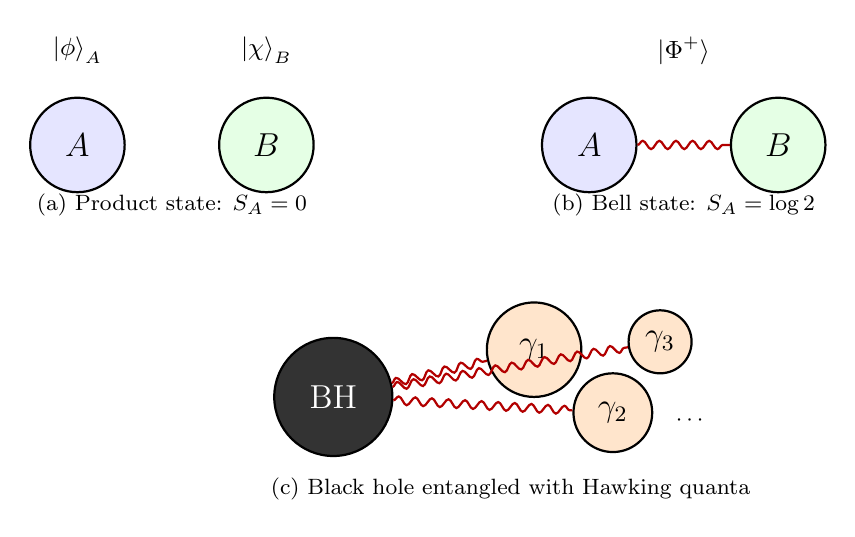
\begin{tikzpicture}[
    qubit/.style={circle, draw, thick, minimum size=1.2cm, font=\large},
    entline/.style={decorate, decoration={snake, amplitude=1.5pt, segment length=6pt}, thick, red!70!black},
    labelstyle/.style={font=\small},
    >=stealth
  ]
  \node[qubit, fill=blue!10] (A1) at (0,0) {$A$};
  \node[qubit, fill=green!10] (B1) at (2.4,0) {$B$};
  \node[labelstyle, above=0.3cm of A1] {$\ket{\phi}_A$};
  \node[labelstyle, above=0.3cm of B1] {$\ket{\chi}_B$};
  \node[font=\footnotesize, below=0.5cm] at (1.2,0) {(a) Product state: $S_A = 0$};

  \node[qubit, fill=blue!10] (A2) at (6.5,0) {$A$};
  \node[qubit, fill=green!10] (B2) at (8.9,0) {$B$};
  \draw[entline] (A2) -- (B2);
  \node[labelstyle, above=0.3cm] at (7.7,0.6) {$\ket{\Phi^+}$};
  \node[font=\footnotesize, below=0.5cm] at (7.7,0) {(b) Bell state: $S_A = \log 2$};

  \node[qubit, fill=black!80, text=white, minimum size=1.5cm] (BH) at (3.25,-3.2) {BH};
  \node[qubit, fill=orange!20, minimum size=1.2cm] (R1) at (5.8,-2.6) {$\gamma_1$};
  \node[qubit, fill=orange!20, minimum size=1.0cm] (R2) at (6.8,-3.4) {$\gamma_2$};
  \node[qubit, fill=orange!20, minimum size=0.8cm] (R3) at (7.4,-2.5) {$\gamma_3$};
  \node[font=\footnotesize] at (7.8, -3.5) {$\cdots$};
  \draw[entline] (BH) -- (R1);
  \draw[entline] (BH) -- (R2);
  \draw[entline] (BH) -- (R3);
  \node[font=\footnotesize, below=0.3cm] at (5.5,-3.8) {(c) Black hole entangled with Hawking quanta};
\end{tikzpicture}
\end{adjustbox}
\caption{Entanglement illustrated.  (a)~In a product state, each subsystem is
independently well-defined and has zero entropy.  (b)~In the Bell state
$\ket{\Phi^+}$, the total system is pure, but each subsystem is maximally mixed
with entropy $\log 2$ (wavy line denotes entanglement).  (c)~A black hole entangled
with its Hawking radiation: each emitted quantum $\gamma_i$ is entangled with
the interior, making the radiation appear thermal when examined in isolation.}
\label{fig02:entanglement}
\end{figure}

\medskip
\noindent\textbf{Monogamy of entanglement.}
A qubit that is maximally entangled with one system \emph{cannot} be entangled with
any other system.  More precisely, if $A$ and $B$ share a Bell state, then $A$ is
completely uncorrelated with any third system~$C$.  This is the \emph{monogamy of
entanglement}, and it is a theorem, not a choice \cite{coffmanetal2000}.

Monogamy is what makes the black hole information paradox genuinely sharp.  If
the entropy of the accumulated radiation decreases after an emission, the
new radiation has negative conditional entropy relative to the earlier
radiation. A smooth horizon also requires the outgoing mode to have the
appropriate near-vacuum correlations with interior modes. Treating these
as independent subsystems leads to competing entanglement requirements.  Monogamy forbids both at once---the ``AMPS firewall''
argument \cite{ampsetal2013} makes this tension precise.

\medskip
\noindent\textbf{EPR and nonlocality.}
The correlations in a Bell state are ``nonlocal'' in the sense that they cannot be
reproduced by any \emph{local hidden variable} theory---this is Bell's theorem
\cite{bell1964}.  However, these correlations do not permit faster-than-light
signalling; the reduced state of each subsystem is the same regardless of what
measurement is performed on the other.  The tension between nonlocal correlations
and the impossibility of signalling is one of the deep conceptual puzzles of
quantum mechanics, but it is not our primary concern in this paper.  What matters
for us is the entanglement structure itself and the entropy it generates for
subsystems.

\subsection{The density matrix}
\label{subsec02:density_matrix}

So far we have described quantum states as vectors $\ket{\psi}\in\Hcal$.  This
description is complete when the system is in a \emph{pure} state.  But in
practice---and this is the norm in black hole physics---we often deal with systems
that are either (a)~part of a larger entangled system, or (b)~prepared with
classical uncertainty about which quantum state they are in.  In both cases, the
appropriate description is the \emph{density matrix} (or density operator).

\medskip
\noindent\textbf{Pure states.}
Given a pure state $\ket{\psi}$, the density matrix is the projector
\begin{equation}\label{eq02:pure_density}
  \rho \;=\; \ket{\psi}\bra{\psi}\,.
\end{equation}
This is a Hermitian, positive semi-definite, trace-one operator on~$\Hcal$.
A pure-state density matrix satisfies
\begin{equation}\label{eq02:pure_condition}
  \rho^2 = \rho\,,
  \qquad
  \tr(\rho^2) = 1\,,
  \qquad
  S(\rho) = 0\,,
\end{equation}
where $S(\rho)$ is the von Neumann entropy defined in
Section~\ref{subsec02:von_neumann}.  Purity ($\rho^2=\rho$) is the density-matrix
equivalent of ``we know the state exactly.''

\medskip
\noindent\textbf{Mixed states.}
Suppose we have classical uncertainty: the system is in state $\ket{\psi_i}$ with
probability $p_i$ (with $p_i\geq 0$, $\sum_i p_i = 1$).  The density matrix is
\begin{equation}\label{eq02:mixed_density}
  \rho \;=\; \sum_i p_i \ket{\psi_i}\bra{\psi_i}\,.
\end{equation}
If the occupied vectors are not all the same ray, this gives a mixed state,
with $\rho^2 \neq \rho$ and $\tr(\rho^2)<1$.  The von Neumann entropy
is strictly positive: $S(\rho)>0$.  The inequality $\tr(\rho^2)<1$ is a useful
diagnostic of mixedness and is directly related to the second R\'{e}nyi entropy
(Section~\ref{subsec02:von_neumann}).

\medskip
\noindent\textbf{The reduced density matrix and the partial trace.}
Consider a bipartite pure state $\ket{\psi}_{AB}\in\Hcal_A\otimes\Hcal_B$.  The
\emph{reduced density matrix} of subsystem~$A$ is obtained by \emph{tracing out}~$B$:
\begin{equation}\label{eq02:partial_trace}
  \rho_A \;=\; \tr_B\bigl(\ket{\psi}\bra{\psi}\bigr)
  \;=\; \sum_j \bra{j}_B \ket{\psi}\bra{\psi}\ket{j}_B\,,
\end{equation}
where $\{\ket{j}_B\}$ is any orthonormal basis for $\Hcal_B$.  The reduced density
matrix $\rho_A$ encodes \emph{all} information that is accessible to an observer
who can only make measurements on~$A$.

Let us compute the reduced density matrix for the Bell state~\eqref{eq02:bell_state}.
Writing $\ket{\Phi^+} = \frac{1}{\sqrt{2}}(\ket{0}_A\ket{0}_B + \ket{1}_A\ket{1}_B)$,
we have
\begin{align}\label{eq02:bell_reduced}
  \rho_A &= \tr_B\bigl(\ket{\Phi^+}\bra{\Phi^+}\bigr) \nonumber\\
  &= \frac{1}{2}\bigl(\ket{0}\bra{0} + \ket{1}\bra{1}\bigr)
  \;=\; \frac{\mathbb{1}_A}{2}\,,
\end{align}
the \emph{maximally mixed state} on qubit~$A$.  By symmetry, $\rho_B =
\mathbb{1}_B/2$ as well.

\medskip
\noindent\textbf{Key property: equal subsystem entropies.}
For any pure state $\ket{\psi}_{AB}$ of a bipartite system, the reduced density
matrices $\rho_A$ and $\rho_B$ have the same nonzero eigenvalues.  Consequently,
\begin{equation}\label{eq02:equal_entropies}
  S(\rho_A) \;=\; S(\rho_B)\,.
\end{equation}
This is a straightforward consequence of the Schmidt decomposition and will play a
starring role in the Page curve: the entropy of the radiation equals the entropy of
the remaining black hole, provided the total state is pure.

\medskip
\noindent\textbf{The maximally mixed state.}
On a $d$-dimensional Hilbert space, the maximally mixed state is
\begin{equation}\label{eq02:max_mixed}
  \rho_{\mathrm{max}} \;=\; \frac{\mathbb{1}}{d}\,,
  \qquad
  S(\rho_{\mathrm{max}}) = \log d\,.
\end{equation}
This is the state of maximum ignorance---every outcome in any orthonormal-basis measurement is equally likely.  It is
the density matrix describing one half of a maximally entangled state of two
$d$-dimensional systems.

\begin{figure}[t]
\centering
\begin{adjustbox}{max width=\textwidth, center}
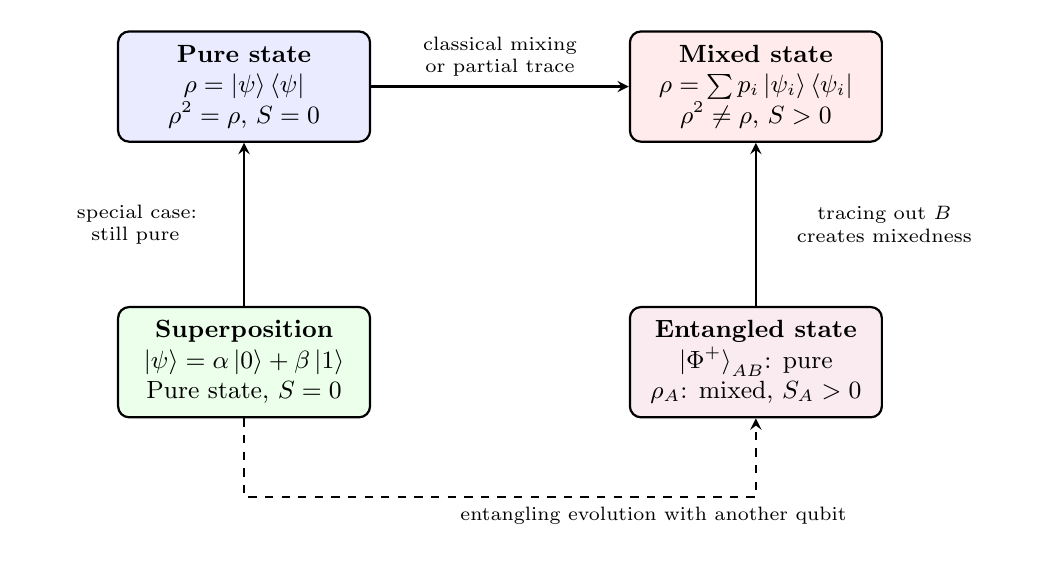
\begin{tikzpicture}[
    box/.style={draw, thick, rounded corners, minimum width=3.2cm, minimum height=1.4cm,
                align=center, font=\small},
    arrow/.style={->, thick, >=stealth},
    note/.style={font=\scriptsize, text width=3.5cm, align=center}
  ]
  \node[box, fill=blue!8] (pure) at (0, 0)
    {\textbf{Pure state}\\$\rho = \ket{\psi}\bra{\psi}$\\$\rho^2=\rho$, $S=0$};
  \node[box, fill=red!8] (mixed) at (6.5, 0)
    {\textbf{Mixed state}\\$\rho = \sum p_i\ket{\psi_i}\bra{\psi_i}$\\$\rho^2\neq\rho$, $S>0$};
  \node[box, fill=green!8] (super) at (0, -3.5)
    {\textbf{Superposition}\\$\ket{\psi}=\alpha\ket{0}+\beta\ket{1}$\\Pure state, $S=0$};
  \node[box, fill=purple!8] (entangled) at (6.5, -3.5)
    {\textbf{Entangled state}\\$\ket{\Phi^+}_{AB}$: pure\\$\rho_A$: mixed, $S_A>0$};

  \draw[arrow] (pure) -- (mixed) node[midway, above, note] {classical mixing\\or partial trace};
  \draw[arrow] (super) -- (pure) node[midway, left, note, text width=2.5cm] {special case:\\still pure};
  \draw[arrow] (entangled.north) -- (mixed.south)
    node[midway, right, note, text width=3cm] {tracing out $B$\\creates mixedness};
  \draw[arrow, dashed] (super.south) -- ++(0,-1.0) -| (entangled.south)
    node[pos=0.4, below, font=\scriptsize] {entangling evolution with another qubit};

\end{tikzpicture}
\end{adjustbox}
\caption{The taxonomy of quantum states.  A superposition is a pure state with zero
entropy.  A mixture has positive entropy and arises either from classical ignorance
or from tracing out part of an entangled system.  The key insight: entanglement of
a pure bipartite state forces each subsystem to be mixed.  This mechanism is exactly
what makes Hawking radiation appear thermal.}
\label{fig02:state_taxonomy}
\end{figure}

\medskip
\noindent\textbf{Pure vs.\ mixed vs.\ superposition: the critical distinction.}
Figure~\ref{fig02:state_taxonomy} summarises the relationships.  A superposition
$\ket{\psi} = \alpha\ket{0}+\beta\ket{1}$ is a \emph{pure} state---it has a density
matrix $\rho=\ket{\psi}\bra{\psi}$ with $\rho^2=\rho$ and $S=0$.  A mixture
$\rho = |\alpha|^2\ket{0}\bra{0} + |\beta|^2\ket{1}\bra{1}$ has $S>0$ when both coefficients are nonzero. Physically,
the superposition displays interference effects (e.g., in a double-slit experiment)
while the mixture does not.

This distinction is the heart of the information paradox.  Hawking's original
calculation \cite{hawking1975} yields radiation described by a thermal density
matrix---a \emph{mixed} state with $S>0$.  If the black hole formed from a pure
initial state, unitarity demands that the final state (after complete evaporation) be
pure.  Resolving the paradox means explaining how a process that appears to produce
mixed-state radiation can ultimately be consistent with purity.

\subsection{Von Neumann entropy and R\'{e}nyi entropies}
\label{subsec02:von_neumann}

We now introduce the entropy measures that quantify the amount of entanglement or
ignorance encoded in a density matrix.

\medskip
\noindent\textbf{Von Neumann entropy.}
The von Neumann entropy of a density matrix~$\rho$ with eigenvalues $\{\lambda_i\}$ is
\begin{equation}\label{eq02:von_neumann}
  S_{\mathrm{vN}}(\rho) \;=\; -\tr(\rho\log\rho)
  \;=\; -\sum_i \lambda_i \log\lambda_i\,,
\end{equation}
where $0\log 0 \equiv 0$ by continuity.  (Throughout this paper, ``$\log$'' denotes
the natural logarithm unless otherwise stated.)  Key properties:
\begin{enumerate}[label=(\alph*),itemsep=2pt]
\item $S\geq 0$, with equality if and only if $\rho$ is pure.
\item $S\leq \log d$ (where $d=\dim\Hcal$), with equality if and only if $\rho$ is
maximally mixed.
\item For a bipartite pure state, $S(\rho_A) = S(\rho_B)$
(Eq.~\eqref{eq02:equal_entropies}).
\item \emph{Strong subadditivity:} $S(\rho_{ABC})+S(\rho_B) \leq
S(\rho_{AB})+S(\rho_{BC})$ \cite{liebruskai1973}.
\item \emph{Araki--Lieb inequality:} $|S(\rho_A)-S(\rho_B)|\leq S(\rho_{AB})$
\cite{arakilieb1970}.
\end{enumerate}
The von Neumann entropy is the quantum analogue of the Shannon entropy.  When $\rho$
describes one half of a bipartite pure state, $S(\rho)$ measures the \emph{entanglement
entropy}---the amount of quantum correlation between the two halves.

\medskip
\noindent\textbf{R\'{e}nyi entropies.}
The R\'{e}nyi entropies are a one-parameter family that generalises the von Neumann
entropy:
\begin{equation}\label{eq02:renyi}
  S_n(\rho) \;=\; \frac{1}{1-n}\,\log\tr(\rho^n)\,,
  \qquad n > 0,\; n\neq 1\,.
\end{equation}
In the limit $n\to 1$, L'H\^{o}pital's rule recovers the von Neumann entropy:
\begin{equation}\label{eq02:renyi_limit}
  \lim_{n\to 1} S_n(\rho) \;=\; S_{\mathrm{vN}}(\rho)\,.
\end{equation}
Several special cases deserve mention.

\begin{itemize}[itemsep=2pt]
\item \textbf{$S_{0^+}(\rho) = \log(\text{rank}\,\rho)$:} the Hartley entropy, counting the
number of nonzero eigenvalues (defined as the limit $n \to 0^+$ of
Eq.~\eqref{eq02:renyi}); the notation $S_{0^+}$ here is distinct from the
JT topological entropy $S_0$.
\item \textbf{$S_2 = -\log\tr(\rho^2)$:} the collision entropy.  Here
$\tr(\rho^2)$ is the \emph{purity} of $\rho$; a pure state has $\tr(\rho^2)=1$
and $S_2=0$, while a maximally mixed state in $d$ dimensions has $\tr(\rho^2)=1/d$
and $S_2=\log d$.  The second R\'{e}nyi entropy is experimentally accessible
\cite{islametal2015} and computationally convenient.
\item \textbf{$S_\infty = -\log\lambda_{\max}$:} the min-entropy, determined by the
largest eigenvalue.
\end{itemize}

\medskip
\noindent\textbf{Why the replica trick works.}
The quantity $\tr(\rho^n)$ for \emph{integer}~$n\geq 2$ can be computed by considering
$n$ identical copies (``replicas'') of the system and sewing them together in a cyclic
pattern.  In the gravitational context, this procedure has a beautiful geometric
interpretation: each replica is a copy of the spacetime, and $\tr(\rho^n)$ is computed
by a path integral over $n$-fold branched cover geometries.  The sum over topologically
distinct ways of connecting these replicas gives rise to \emph{replica wormholes}, which
are the key to deriving the Page curve from semiclassical gravity.  We will develop
this idea in detail in Section~\ref{sec06:replica_wormholes}.

The strategy is:
\begin{enumerate}[label=\arabic*.,itemsep=1pt]
\item Compute $\tr(\rho^n)$ for integer $n\geq 2$ using the replica method.
\item Analytically continue in~$n$ to a neighbourhood of $n=1$.
\item Take the limit $n\to 1$ to extract $S_{\mathrm{vN}}$.
\end{enumerate}
This procedure is the \emph{replica trick}. Integer values alone do not
specify an analytic continuation without additional assumptions. For a known
finite-dimensional density matrix, its spectrum directly defines
$\tr\rho^n$ for real $n>0$. In a saddle-point calculation one must also
control continuation and the order of limits. Carlson-type uniqueness
conditions can be checked for the flat-weight spectral benchmark discussed
in Section~\ref{sec07:free_probability}; they are not a general theorem
about the full gravitational replica path integral.

\medskip
\noindent\textbf{The entanglement spectrum.}
The full set of eigenvalues $\{\lambda_i\}$ of a reduced density matrix is called
the \emph{entanglement spectrum}.  The von Neumann entropy is a single number extracted
from this spectrum; the R\'{e}nyi entropies form a one-parameter family.  But the
spectrum itself contains strictly more information than any single entropy.

Section~\ref{sec07:free_probability} derives the Marchenko--Pastur
limit for a normalized flat-weight random state. In a gravitational
application, identifying this law requires the corresponding preparation
and weights. Later chapters distinguish a spectrum in one realization,
an averaged spectral density, and correlations between eigenvalues in
an ensemble. None of these spectra includes eigenvectors, and therefore
none alone specifies every observable or the dynamics of a state.

\subsection{Unitarity and the no-information-loss principle}
\label{subsec02:unitarity}

The time evolution of an isolated quantum system is governed by a \emph{unitary}
operator:
\begin{equation}\label{eq02:unitary_evolution}
  \ket{\psi(t)} \;=\; U(t)\ket{\psi(0)}\,,
  \qquad U^\dagger U = U U^\dagger = \mathbb{1}\,.
\end{equation}
Unitarity is an extraordinarily powerful constraint.  It preserves:
\begin{enumerate}[label=(\roman*),itemsep=2pt]
\item \textbf{Inner products:} $\braket{\phi(t)|\psi(t)} = \braket{\phi(0)|\psi(0)}$.
Two states that start out distinguishable remain distinguishable forever.

\item \textbf{Purity:} If $\rho(0) = \ket{\psi(0)}\bra{\psi(0)}$ is pure, then
$\rho(t) = U(t)\rho(0)U^\dagger(t)$ is also pure.

\item \textbf{Entropy:} $S(\rho(t)) = S(\rho(0))$.  The von Neumann entropy of
the total system is a constant of the motion.

\item \textbf{Information:} Since $U$ is invertible, the initial state can in principle be
recovered when the unitary is known and its inverse can be implemented: $\ket{\psi(0)} = U^\dagger(t)\ket{\psi(t)}$.
No information is ever destroyed.
\end{enumerate}

The preservation of information under unitary evolution is sometimes called the
\emph{no-information-loss principle}.  In the context of the gravitational path
integral, it is the statement that quantum gravity---whatever its ultimate
formulation---must be a unitary theory.

\medskip
\noindent\textbf{The key constraint for black holes.}
Suppose a black hole forms from the collapse of a pure quantum state
$\ket{\psi_{\mathrm{initial}}}$---say, a shell of photons in a definite quantum
state.  The black hole then evaporates completely via Hawking radiation.  If
quantum mechanics is unitary, then the final state of the radiation must also be
pure:
\begin{equation}\label{eq02:unitarity_constraint}
  \ket{\psi_{\mathrm{initial}}} \;\xrightarrow{\;\;U\;\;}
  \;\ket{\psi_{\mathrm{radiation}}}\,,
  \qquad
  S(\rho_{\mathrm{radiation}}) = 0\,.
\end{equation}
This is a strong statement.  It says that all the information that went
into forming the black hole must come out in the Hawking radiation.  The radiation
may look thermal to any practical measurement, but it must be in a \emph{globally
pure} state---an astronomically complicated superposition whose correlations encode
the initial state.

\medskip
\noindent\textbf{Why physicists take unitarity so seriously.}
One might ask: why not simply accept that black holes destroy information?
Several lines of argument militate against this:

\begin{enumerate}[label=(\alph*),itemsep=2pt]
\item \textbf{Energy conservation violation.}  Banks, Susskind, and Peskin
\cite{banks1984} analyzed serious tensions between local nonunitary modifications and
energy conservation. The conclusion depends on the form of the proposed
evolution; it is not a theorem that every nonunitary quantum channel violates
energy conservation.

\item \textbf{AdS/CFT.}  In the AdS/CFT correspondence \cite{maldacena1998}, the
boundary conformal field theory is manifestly unitary.  If the correspondence is
exact, then the bulk gravitational theory---including black hole formation and
evaporation---must also be unitary.

\item \textbf{Universal structure of quantum mechanics.}  Unitary Hamiltonian evolution is the standard description of a closed
system. Open systems admit nonunitary, trace-preserving channels while
retaining consistent probabilities. Fundamental information loss would
therefore require changing the closed-system dynamical postulate, rather
than following merely from a different description of a subsystem.
\end{enumerate}

The tension between Hawking's apparently thermal radiation (mixed state, $S>0$) and
the demand of unitarity (pure final state, $S=0$) is the black hole information
paradox.  Resolving this tension---and understanding the detailed mechanism by which
information escapes---is the driving question of this paper.

\bigskip
\noindent\textbf{Summary.}
We have assembled the following toolkit:
\begin{itemize}[itemsep=1pt]
\item Quantum states live in Hilbert spaces.  A black hole's entropy estimates the logarithm of the number of states in
a suitable energy window.
\item Composite systems have tensor-product Hilbert spaces.  Entanglement is the rule,
not the exception.
\item The Bell state illustrates the core phenomenon: a globally pure state whose
subsystems are maximally mixed.  Entanglement creates ignorance.
\item The density matrix describes both pure and mixed states.  The partial trace over
one subsystem produces the reduced density matrix.
\item For a pure bipartite state, subsystem von Neumann entropy quantifies
entanglement. R\'{e}nyi entropies give additional spectral information;
eigenvectors and channel data contain information beyond a spectrum.
\item Unitarity preserves purity and information.  A pure initial state must evolve to a
pure final state.
\end{itemize}
Armed with this language, we are ready to introduce black holes and confront the
paradox directly in Section~\ref{sec03:black_holes}.


\section{Black Holes and Hawking Radiation}\label{sec03:black_holes}

The previous section established the quantum-mechanical toolkit---density
matrices, entanglement entropy, and the unitarity constraint---that we will need
throughout this paper.  We now turn to the gravitational arena in which all of those
concepts are pushed to their breaking point: the physics of black holes.  Our
goal in this section is threefold.  First, we introduce the classical black hole
as a solution of Einstein's equations, emphasizing the features---event
horizons, the no-hair theorem---that make the information problem conceivable.
Second, we develop the thermodynamic picture due to Bekenstein and Hawking that
assigns entropy and temperature to a black hole.  Third, we explain Hawking's
celebrated 1975 calculation of thermal radiation and trace its logic to its
alarming conclusion: a violation of unitarity, the central principle of quantum
mechanics.  By the end of this section, the reader should understand the
information paradox as a \emph{precise} conflict between general relativity and
quantum mechanics, and see how a Page curve tests the resulting entropy calculation.

\subsection{Black holes in a nutshell}\label{subsec03:nutshell}

In an asymptotically flat classical spacetime, a black hole is the region
that cannot send a signal to future null infinity.  The boundary of that region is the \textbf{event horizon},
a null hypersurface that acts as a one-way membrane: signals can cross inward
but never outward.

\paragraph{The Schwarzschild solution.}
The simplest black hole is the Schwarzschild solution, discovered in 1916
\cite{schwarzschild1916}.  For a non-rotating, uncharged mass $M$, the metric
in Schwarzschild coordinates reads
\begin{equation}\label{eq03:schwarzschild}
  ds^{2} \;=\; -\!\left(1 - \frac{r_{s}}{r}\right) dt^{2}
  + \left(1 - \frac{r_{s}}{r}\right)^{-1} dr^{2}
  + r^{2}\, d\Omega_{2}^{2}\,,
\end{equation}
where $r_{s} = 2G_{N}M$ is the Schwarzschild radius (in units with $c = 1$;
we set $\hbar = c = k_{B} = 1$ throughout this section) and $d\Omega_{2}^{2}$
is the round metric on $S^{2}$.  The coordinate singularity at $r = r_{s}$
is the event horizon; it can be removed by passing to Kruskal--Szekeres
coordinates, confirming that nothing physically singular happens at the
horizon itself.  The true curvature singularity at $r = 0$ is physical and
signals the breakdown of classical general relativity.

\paragraph{The event horizon as a causal boundary.}
The defining property of the horizon is \emph{causal}: it is the boundary
of the past of future null infinity, $\mathcal{H}^{+} = \partial
J^{-}(\mathscr{I}^{+})$.  An observer freely falling through the horizon
notices nothing locally dramatic---tidal forces are small for a
sufficiently massive black hole, scaling as $M^{-2}$.  Yet an observer
hovering outside sees the infalling object asymptotically redshift and
freeze at the horizon, never quite crossing it.  This tension between the
local and global descriptions will reappear forcefully when we discuss the
information paradox.

\paragraph{The no-hair theorem.}
One of the most striking features of classical black holes is their
extreme simplicity.  The \emph{no-hair theorem} (more precisely, a
collection of uniqueness results \cite{israel1967,israel1968,carter1971})
states, under suitable regularity, asymptotic-flatness, and connected-horizon
assumptions, that a stationary black hole in four-dimensional
Einstein--Maxwell theory is characterized by
its mass $M$, electric charge $Q$, and angular momentum $J$.
No other internal structure is visible from outside the horizon.  The
most general such solution is the Kerr--Newman metric.

This radical simplicity has a direct bearing on the information problem.
If a black hole is formed from the gravitational collapse of, say, a
library of books, all information about the contents of those books is
hidden behind the horizon.  The external spacetime is indistinguishable
from one formed by the collapse of an equal mass of iron filings.  Where
did the information go?  Classically, the answer is straightforward:
it fell behind the horizon and remains there.  But as we shall see,
Hawking's discovery of black hole radiation reopens the question in a
dramatic way.

\paragraph{Penrose diagrams.}
The causal structure of a black hole spacetime is most transparently
displayed in a \emph{Penrose (conformal) diagram} \cite{penrose1963},
which compactifies the infinite spacetime onto a finite region while
preserving the light-cone structure.  Figure~\ref{fig03:penrose} shows the Penrose
diagram for a black hole formed from gravitational collapse and
subsequently evaporating via Hawking radiation.  The key features are:
(i) the collapsing matter (shaded region) that forms the horizon;
(ii) the event horizon itself, a null surface;
(iii) the singularity at the top;
(iv) future null infinity $\mathscr{I}^{+}$, where the Hawking radiation
is collected; and (v) the endpoint of evaporation, after which the
spacetime returns to flat Minkowski space (in the idealized picture).

\begin{figure}[ht]
\centering
\begin{adjustbox}{max width=\textwidth, center}
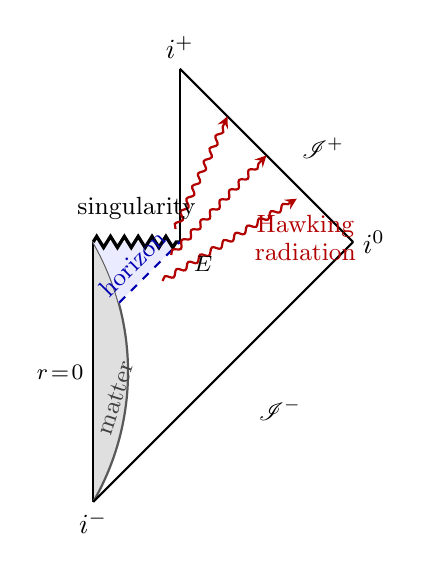
\begin{tikzpicture}[scale=1.1]

  \coordinate (iminus) at (0, 0);
  \coordinate (izero)  at (3, 3);
  \coordinate (iplus)  at (1, 5);
  \coordinate (E)      at (1, 3);
  \coordinate (S)      at (0, 3);

  \fill[gray!25]
    (iminus) arc[start angle=-30, end angle=30, radius=3] -- (S)
    -- (0,0) -- cycle;
  \draw[thick] (iminus) -- (S);
  \draw[thick, gray!70!black]
    (iminus) arc[start angle=-30, end angle=30, radius=3];

  \fill[blue!8] (0.3, 2.3) -- (E) -- (S)
    -- (S) arc[start angle=30, end angle=15.4, radius=3] -- cycle;

  \draw[thick] (E) -- (iplus);

  \draw[thick] (iminus) -- (izero);

  \draw[thick] (izero) -- (iplus);

  \draw[decorate, decoration={zigzag, segment length=5pt, amplitude=2pt},
        very thick] (S) -- (E);

  \draw[dashed, thick, blue!70!black] (0.3, 2.3) -- (E);

  \draw[-stealth, red!70!black, thick,
        decorate, decoration={snake, amplitude=1pt, segment length=5pt,
        post length=3pt}]
    (0.8, 2.55) -- (2.35, 3.5);
  \draw[-stealth, red!70!black, thick,
        decorate, decoration={snake, amplitude=1pt, segment length=5pt,
        post length=3pt}]
    (0.9, 2.85) -- (2.0, 4.0);
  \draw[-stealth, red!70!black, thick,
        decorate, decoration={snake, amplitude=1pt, segment length=5pt,
        post length=3pt}]
    (0.95, 3.15) -- (1.55, 4.45);

  \node[below]       at (iminus) {$i^{-}$};
  \node[right]       at (izero)  {$i^{0}$};
  \node[above]       at (iplus)  {$i^{+}$};

  \node[below right, font=\footnotesize] at (1.05, 2.95) {$E$};

  \node[above, font=\small] at (0.5, 3.15) {singularity};

  \node[below right, font=\small] at (1.8, 1.3) {$\mathscr{I}^{-}$};
  \node[above right, font=\small] at (2.3, 3.85) {$\mathscr{I}^{+}$};

  \node[rotate=45, blue!70!black, font=\small, above] at (0.6, 2.6)
    {horizon};

  \node[left, font=\footnotesize] at (0, 1.5) {$r\!=\!0$};

  \node[gray!50!black, font=\small, rotate=72] at (0.25, 1.2) {matter};

  \node[red!70!black, font=\small, align=center] at (2.45, 3.05)
    {Hawking\\[-1pt]radiation};

\end{tikzpicture}
\end{adjustbox}
\caption{Penrose diagram for a black hole formed by gravitational
collapse and evaporating via Hawking radiation.  Light travels at
$45^{\circ}$.  The gray region is the collapsing matter (between the
stellar surface and the $r\!=\!0$ axis).  The dashed blue line is the
event horizon; the zigzag line is the spacelike singularity.  After
complete evaporation at~$E$, the spacetime returns to flat Minkowski
geometry.  Hawking quanta (wavy red arrows) propagate to future null
infinity~$\mathscr{I}^{+}$.  The light-blue interior is causally
disconnected from~$\mathscr{I}^{+}$---the heart of the information
paradox.}
\label{fig03:penrose}
\end{figure}

\subsection{Black hole thermodynamics}\label{subsec03:thermodynamics}

The first hint that black holes are more than classical geometric objects
came from a set of formal analogies---later understood to be exact
identities---between the laws governing black hole mechanics and the laws of
thermodynamics.  These were developed in the early 1970s through the work of
Bekenstein \cite{bekenstein1973}, Bardeen, Carter, and Hawking
\cite{bardeenetal1973}, and others.

\subsubsection*{The four laws of black hole mechanics}

The analogy is summarized in Table~\ref{tab03:four_laws}.

\begin{table}[ht]
\centering
\caption{The four laws of black hole mechanics and their thermodynamic
counterparts.  The surface gravity $\kappa$ plays the role of temperature,
and the horizon area $A$ plays the role of entropy.}
\label{tab03:four_laws}
\begin{adjustbox}{max width=\textwidth,center}
\begin{tabular}{@{}lll@{}}
\toprule
\textbf{Law} & \textbf{Thermodynamics} & \textbf{Black hole mechanics} \\
\midrule
Zeroth & $T$ is constant in equilibrium & $\kappa$ is constant on the horizon \\
First  & $dE = T\, dS + \text{work}$ & $dM = \frac{\kappa}{8\pi G_{N}}\, dA + \Omega\, dJ + \Phi\, dQ$ \\
Second & $\delta S \geq 0$ & $\delta A \geq 0$ (area theorem) \\
Third  & $T = 0$ not reachable & $\kappa = 0$ not reachable \\
\bottomrule
\end{tabular}
\end{adjustbox}
\end{table}

The second law---Hawking's area theorem \cite{hawking1971area}---states
that, under the null energy condition and appropriate global causal
assumptions, event-horizon area cannot decrease in classical evolution.  This was the clue that first led Bekenstein to propose
that a black hole carries entropy proportional to its area.

\subsubsection*{Bekenstein--Hawking entropy}

Bekenstein \cite{bekenstein1973} proposed that a black hole carries an
entropy proportional to its horizon area, with a coefficient he could
estimate only up to a factor of order one; Hawking's temperature
calculation \cite{hawking1975} then fixed the coefficient, yielding the
\emph{Bekenstein--Hawking entropy}
\begin{equation}\label{eq03:bekenstein_entropy}
  S_{\mathrm{BH}} \;=\; \frac{A}{4\, G_{N}}\,,
\end{equation}
where $A$ is the area of the event horizon and we work in units with
$\hbar = c = k_{B} = 1$.  For a Schwarzschild black hole of mass $M$,
the horizon area is $A = 16\pi G_{N}^{2} M^{2}$, giving
\begin{equation}\label{eq03:sbh_schwarzschild}
  S_{\mathrm{BH}} \;=\; 4\pi G_{N} M^{2}\,.
\end{equation}

The Bekenstein--Hawking entropy is enormous.  A solar-mass black hole has
$S_{\mathrm{BH}} \sim 10^{77}$, vastly exceeding the entropy of the
star from which it formed.  This is one of several hints that the
number of states in a narrow black-hole energy window satisfies, to
leading semiclassical order,
\begin{equation}\label{eq03:hilbert_dim}
  \log \dim \Hcal_{\mathrm{BH},E} \;\simeq\; S_{\mathrm{BH}}(E)\,,
\end{equation}
corresponding to an exponentially large state count, despite the no-hair theorem telling us
that the \emph{external} description involves only three parameters.
The tension between the simplicity of the exterior and the enormous
number of microstates suggested by the entropy is a recurring theme.

\paragraph{Why area and not volume?}
In ordinary thermodynamic systems, entropy is an extensive quantity
scaling with the volume.  The Bekenstein--Hawking entropy, by contrast, scales
with the \emph{area} of the horizon.  This is the first appearance
of the \textbf{holographic principle}---the idea that the maximum
entropy in a region of space scales with the boundary area rather than
the bulk volume \cite{thooft1993,susskind1995}.  We will see this
principle realized concretely in the AdS/CFT correspondence
(Section~\ref{sec04:holography}).

\subsubsection*{Hawking temperature}

Having established the analogy between $\kappa$ and temperature,
the natural question is: what is the \emph{actual} temperature?
Hawking's 1975 calculation \cite{hawking1975} answered this definitively.
A black hole radiates thermally at the \textbf{Hawking temperature}
\begin{equation}\label{eq03:hawking_temp}
  T_{H} \;=\; \frac{\kappa}{2\pi}\,,
\end{equation}
where $\kappa$ is the surface gravity.  For a Schwarzschild black hole,
$\kappa = 1/(4G_{N}M)$, so
\begin{equation}\label{eq03:hawking_temp_schwarz}
  T_{H} \;=\; \frac{1}{8\pi G_{N} M}\,.
\end{equation}
Note the inverse relationship with mass: \emph{smaller black holes are
hotter}.  This has the dramatic consequence that Hawking radiation is a
runaway process.  As the black hole radiates and loses mass, it grows
hotter, radiates faster, and eventually---in the absence of new
physics---undergoes complete evaporation in a finite time.

For Einstein gravity at leading semiclassical order, the thermodynamic
identifications are
\begin{equation}\label{eq03:thermo_identifications}
  T = T_{H} = \frac{\kappa}{2\pi}\,, \qquad
  S = S_{\mathrm{BH}} = \frac{A}{4G_{N}}\,.
\end{equation}
These satisfy the first law in the form
\begin{equation}\label{eq03:first_law}
  dM \;=\; T_{H}\, dS_{\mathrm{BH}} + \Omega\, dJ + \Phi\, dQ\,,
\end{equation}
confirming the consistency of the entire thermodynamic framework.

\paragraph{A sanity check: black hole evaporation time.}
The Stefan--Boltzmann law gives the power radiated by a body of
temperature $T$ and area $A$ as $P \sim \sigma T^{4} A$.  Using
$T_{H} \propto M^{-1}$ and $A \propto M^{2}$, one finds
$P \propto M^{-2}$, so $dM/dt \propto -M^{-2}$, giving an
evaporation time
\begin{equation}\label{eq03:evap_time}
  t_{\mathrm{evap}} \;\sim\; G_{N}^{2} M^{3}\,.
\end{equation}
For a solar-mass black hole this is $\sim 10^{67}$ years
\cite{page1976}, far longer than the age of the universe.  The information paradox is therefore
a conceptual rather than observational crisis---but no less sharp for that.

\subsection{Hawking radiation}\label{subsec03:hawking_radiation}

We now turn to the physical mechanism behind Hawking radiation and,
crucially, the entanglement structure it creates.  It is this
entanglement structure that drives the information paradox.

\subsubsection*{The mechanism: particle creation in curved spacetime}

Hawking's original derivation \cite{hawking1975} proceeds by studying a
free quantum field on the background of a collapsing star that forms a
black hole.  The key insight is that the notion of ``particle'' is
observer-dependent in curved spacetime.  The vacuum state defined by
an observer in the far past (before the black hole forms) is not the
same as the vacuum defined by an observer in the far future (after the
horizon has settled down).  The two sets of mode functions are related
by a \textbf{Bogoliubov transformation}:
\begin{equation}\label{eq03:bogoliubov}
  \hat{b}_{\omega} \;=\; \int d\omega'\,
  \bigl(\alpha_{\omega\omega'}\, \hat{a}_{\omega'}
  + \beta_{\omega\omega'}\, \hat{a}_{\omega'}^{\dagger}\bigr)\,,
\end{equation}
where $\hat{a}_{\omega}$ and $\hat{b}_{\omega}$ are annihilation
operators for the ``in'' and ``out'' mode decompositions, and
$\alpha_{\omega\omega'}$ and $\beta_{\omega\omega'}$ are the
Bogoliubov coefficients.  A non-vanishing $\beta$ coefficient means
that the ``in'' vacuum contains ``out'' particles.

The central result of Hawking's calculation is that the number
spectrum of outgoing particles is thermal:
\begin{equation}\label{eq03:planckian}
  \langle \hat{N}_{\omega} \rangle
  \;=\; \frac{1}{e^{\omega / T_{H}} - 1}
  \qquad (\text{bosons})\,,
\end{equation}
a Planck distribution at the Hawking temperature $T_{H}$.  (For
fermions, the minus sign becomes a plus sign, giving a Fermi--Dirac
distribution.  The full result multiplies this occupation number by a
frequency-dependent \emph{greybody factor} $\Gamma_{\omega}$, the
transmission probability through the potential barrier outside the
horizon. It modifies the spectrum measured at infinity while retaining the
Hawking temperature in its occupation factor.)
This thermal spectrum depends only on the mass $M$
of the black hole (and its charge and spin, if present).  At this level of the calculation it does not distinguish microscopic
initial states with the same macroscopic parameters.

\subsubsection*{The entanglement structure of Hawking pairs}

The thermal nature of the radiation has a deeper origin in
\emph{entanglement}.  The Bogoliubov transformation creates particles
in pairs: for each outgoing Hawking quantum at frequency $\omega$
escaping to infinity, there is a partner quantum at frequency $\omega$
that falls behind the horizon.  The joint state of a single Hawking
pair takes the form
\begin{equation}\label{eq03:hawking_pair}
  \ket{\Psi_{\omega}} \;=\;
  \frac{1}{\sqrt{Z}} \sum_{n=0}^{\infty}
  e^{-n\omega/(2T_{H})}\,
  \ket{n}_{\mathrm{out}} \otimes \ket{n}_{\mathrm{in}}\,,
\end{equation}
where $Z = (1 - e^{-\omega/T_{H}})^{-1}$ is the normalization and
$\ket{n}_{\mathrm{out}}$, $\ket{n}_{\mathrm{in}}$ are $n$-particle
states of the outgoing and infalling modes, respectively.  This is a
two-mode squeezed state: tracing over the partner behind the horizon
produces a thermal density matrix for the exterior mode,
\begin{equation}\label{eq03:rho_single_mode}
  \rho_{\mathrm{out}} \;=\; \tr_{\mathrm{in}} \ket{\Psi_{\omega}}
  \!\bra{\Psi_{\omega}}
  \;=\; \frac{1}{Z} \sum_{n} e^{-n\omega/T_{H}} \ket{n}\!\bra{n}\,,
\end{equation}
which is exactly a thermal (Gibbs) state.

Now consider the full radiation field, consisting of many such modes
emitted over the black hole's lifetime.  Each outgoing mode is
entangled with its partner behind the horizon, and these partners are
hidden from any external observer.  As the black hole evaporates and
emits more and more Hawking quanta, the total entanglement entropy of
the radiation grows:
\begin{equation}\label{eq03:svn_monotonic}
  S_{\mathrm{vN}}(\rho_{\mathrm{rad}}) \;\sim\; N_{\mathrm{emitted}}
  \;\sim\; S_{\mathrm{BH}}^{(\mathrm{initial})} - S_{\mathrm{BH}}(t)\,,
\end{equation}
where $N_{\mathrm{emitted}}$ counts emitted quanta and the relation is
parametric, not an equality of coefficients. Entropy production in the outgoing
radiation depends on the species and greybody factors. Extrapolating the
independent-pair approximation gives a monotonically increasing radiation
entropy of order the initial black-hole entropy. The final evaporation stage
is outside the regime of that semiclassical approximation.

This is the crux of the problem.  If the black hole evaporates
completely, the partners behind the horizon are simply gone---there is
no subsystem left to purify the radiation.  The radiation is left in a
\emph{mixed} state even though we assumed the initial state was pure.

\subsection{The information paradox---sharp statement}
\label{subsec03:information_paradox}

We are now in a position to state the black hole information paradox
precisely.  The argument proceeds in three steps.

\paragraph{Step 1: Pure initial state.}
Consider a black hole formed from the gravitational collapse of matter
in a pure quantum state $\ket{\Psi_{0}}$.  (One can imagine collapsing
a shell of photons in a carefully prepared quantum state.)  The total
system---black hole plus radiation---is described by a state in a
Hilbert space $\Hcal_{\mathrm{BH}} \otimes \Hcal_{\mathrm{rad}}$.
At early times, before any radiation has been emitted, the radiation
Hilbert space is trivial and $S_{\mathrm{vN}}(\rho_{\mathrm{rad}}) = 0$.

\paragraph{Step 2: Hawking's calculation.}
As the black hole evaporates, it emits thermal radiation.  The
entanglement between each outgoing Hawking quantum and its infalling
partner causes $S_{\mathrm{vN}}(\rho_{\mathrm{rad}})$ to increase
monotonically, as derived in \eqref{eq03:svn_monotonic}.

\paragraph{Step 3: The final state.}
If the independent-pair description is extrapolated through complete
evaporation, it predicts a mixed radiation state. In an idealized
wave-packet description without greybody scattering, its schematic form is
\begin{equation}\label{eq03:rho_thermal_final}
  \rho_{\mathrm{rad}}^{(\mathrm{final})}
  \;\approx\; \bigotimes_j \frac{e^{-\omega_j N_j/T_H(t_j)}}{Z_j}\,,
\end{equation}
where $j$ labels packets emitted at times $t_j$, $N_j$ is their number
operator, and $Z_j$ normalizes each factor. The temperature changes during
evaporation; a single Gibbs state at one temperature does not describe the
whole history. The mixed result represents an evolution
\begin{equation}\label{eq03:pure_to_mixed}
  \ket{\Psi_{0}}\!\bra{\Psi_{0}} \;\longrightarrow\;
  \rho_{\mathrm{rad}}^{(\mathrm{final})}
  \;\neq\; \ket{\Psi_{f}}\!\bra{\Psi_{f}}
\end{equation}
from a pure state to a mixed state.  Such an evolution \emph{cannot}
be described by any unitary operator.

\subsubsection*{Why this is a real paradox}

One might be tempted to dismiss the information paradox as a technical
subtlety or an artifact of approximations.  It is neither.  The paradox
is a sharp conflict between two of the most well-tested principles in
physics:

\begin{enumerate}[label=(\roman*)]
  \item \textbf{Unitarity of quantum mechanics.}  The evolution of any
  closed quantum system is unitary: pure states evolve to pure states,
  and information is conserved.  This is not a minor technical
  assumption---it is the foundation of the entire quantum-mechanical
  framework, and fundamental modifications face consistency constraints, including
  tensions between locality and energy conservation \cite{banks1984}.
  Nonunitary subsystem channels themselves need not violate probability
  conservation.

  \item \textbf{Validity of semiclassical gravity in low-curvature
  regions.}  Hawking's calculation uses quantum field theory on a
  classical curved background.  The approximation is applied
  \emph{outside} the horizon, where curvature is low (for a massive
  black hole) and we have every reason to trust the semiclassical
  expansion for local observables. The issue is whether this approximation
  also controls the fine-grained entropy of all the radiation, especially
  after contributions from additional replica saddles become relevant.
  Low local curvature alone does not establish that the original entropy
  calculation remains uniformly valid throughout evaporation.
\end{enumerate}

The paradox, then, is not ``we don't know the answer.''  It is that
two individually well-supported principles give contradictory
predictions, and modifying either one comes at an enormous cost.

\subsubsection*{Proposed resolutions (preview)}

Over the four decades following Hawking's 1975 paper, a number of
resolutions were proposed.  We mention them briefly here, deferring
detailed discussion to later sections:

\begin{itemize}
  \item \textbf{Information is truly lost.}  One simply accepts that
  unitarity is violated in quantum gravity.  Hawking himself initially
  advocated this position \cite{hawking1976} but later abandoned it.

  \item \textbf{Remnants.}  The black hole does not evaporate
  completely but leaves behind a stable Planck-scale remnant that
  stores the missing information.  This requires a Planck-mass object
  to have an exponentially large number of internal states, leading to
  serious difficulties with pair production and the species problem
  \cite{giddings1992}.

  \item \textbf{Information comes out in the radiation.}  Unitarity
  is preserved, and the Hawking radiation is not truly thermal---subtle
  correlations encode the information of the initial state.  This is
  the resolution most widely accepted today, and the Page curve
  provides the quantitative benchmark.

  \item \textbf{Fuzzballs.}  The black hole interior is replaced by a
  horizon-scale microstate structure. Explicit smooth horizonless
  solutions realize some sectors; extrapolation to generic black-hole
  states and their complete evaporation remains a separate problem
  \cite{mathur2005}.
\end{itemize}

\subsubsection*{The Page curve as diagnostic}

If a pure initial state evolves unitarily into radiation alone, the final
radiation entropy is zero. If the entropy has grown at intermediate times,
it must subsequently decrease. These facts do not fix its detailed history.  The question is: what does the entropy curve
$S_{\mathrm{vN}}(\rho_{\mathrm{rad}})$ look like as a function of
time?

The answer was provided by Don Page in 1993 \cite{page1993,
page1993information}.  Page modeled the joint state of black hole and
radiation as a \emph{random pure state} on a Hilbert space of dimension
$d_{\mathrm{BH}}\, d_{\mathrm{rad}}$, with $d_{\mathrm{BH}} =
e^{S_{\mathrm{BH}}}$; near-maximal entanglement of the smaller factor
is then a consequence, not an assumption.  Using the result
for the average entanglement entropy of a random subsystem, he
showed that
\begin{equation}\label{eq03:page_curve}
  \boxed{
  S_{\mathrm{vN}}(\rho_{\mathrm{rad}})
  \;\approx\;
  \min\!\bigl(S_{\mathrm{rad}},\; S_{\mathrm{BH}}(t)\bigr)\,,
  }
\end{equation}
where $S_{\mathrm{rad}}$ is the coarse-grained (thermodynamic) entropy
of the emitted radiation and $S_{\mathrm{BH}}(t)$ is the remaining
Bekenstein--Hawking entropy of the black hole.  The key features of
the \textbf{Page curve} are:

\begin{enumerate}
  \item \textbf{Early times} ($t < t_{\mathrm{Page}}$): the radiation
  entropy grows, tracking $S_{\mathrm{rad}} \approx N_{\mathrm{emitted}}$.
  The radiation subsystem is smaller than the black hole, and the
  entropy grows because each new Hawking quantum adds new entanglement.

  \item \textbf{Page time} ($t = t_{\mathrm{Page}}$): the entropy
  is near the crossing of the two coarse-grained entropies. In a
  fixed-total-dimension toy model this occurs at half the initial entropy.
  With irreversible entropy production, the crossing need not occur there.

  \item \textbf{Late times} ($t > t_{\mathrm{Page}}$): the entropy
  \emph{decreases}, now tracking $S_{\mathrm{BH}}(t)$.  The radiation
  is the larger subsystem, and as the black hole shrinks, the maximum
  possible entanglement between the two subsystems decreases.

  \item \textbf{Complete evaporation} ($t = t_{\mathrm{evap}}$): the
  entropy returns to zero.  The radiation is in a pure state,
  consistent with unitary evolution.
\end{enumerate}

A simple evaporation model makes this dependence explicit. Suppose
$dM/dt=-a/M^2$, with constant $a>0$, so that
$S_{\mathrm{BH}}(t)/S_i=(1-t/t_{\mathrm{evap}})^{2/3}$, where
$S_i$ is the initial black-hole entropy. Let $\xi$ be the ratio of
radiation entropy production to the decrease in black-hole entropy:
\begin{equation}
 S_{\mathrm{rad}}(t)=\xi\,[S_i-S_{\mathrm{BH}}(t)].
 \label{eq03:entropy_production}
\end{equation}
For constant $\xi$, equating the branches gives
\begin{equation}
 \frac{S_{\mathrm{BH}}(t_P)}{S_i}=\frac{\xi}{1+\xi},
 \qquad
 \frac{t_P}{t_{\mathrm{evap}}}
 =1-\left(\frac{\xi}{1+\xi}\right)^{3/2}.
 \label{eq03:page_time_xi}
\end{equation}
The choice $\xi=1$ gives $t_P/t_{\mathrm{evap}}\simeq0.6464$.
An ideal massless blackbody flux in three spatial dimensions has
$dS_{\mathrm{rad}}=4\,dE_{\mathrm{rad}}/(3T_H)$, while the first law
has $-dS_{\mathrm{BH}}=dE_{\mathrm{rad}}/T_H$. Thus $\xi=4/3$
in that idealization and $t_P/t_{\mathrm{evap}}\simeq0.5680$.
Actual greybody factors and particle content change $\xi$ and the mass-loss
law \cite{page1976}. Neither numerical time is a consequence of unitarity
alone.

\begin{figure}[ht]
\centering
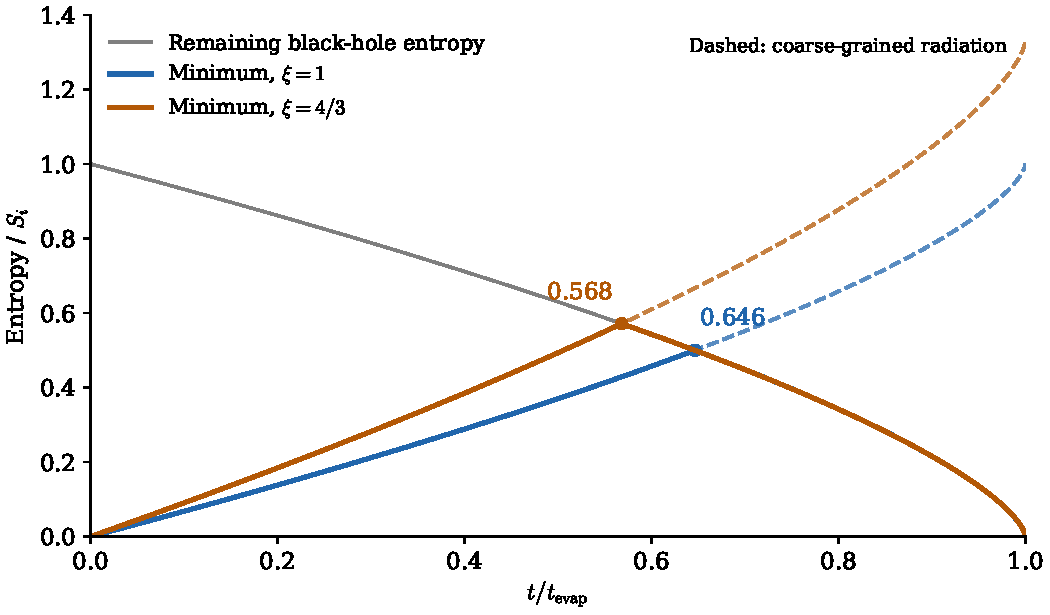
\includegraphics[width=0.88\textwidth]{figures/output/fig03_page_curve.pdf}
\caption{Typical-state entropy benchmarks for the specified mass-loss model.
The black-hole entropy is $(1-t/t_{\mathrm{evap}})^{2/3}$ in units of its
initial value. Solid curves are the minimum of this branch and
$\xi[1-(1-t/t_{\mathrm{evap}})^{2/3}]$; dashed curves are the corresponding
coarse-grained radiation entropies. The choices $\xi=1$ and $4/3$ give
different crossing times. These are model curves, not numerical solutions
of a gravitational evaporation problem. The late endpoint extrapolates
beyond the semiclassical regime.}
\label{fig03:page_curve}
\end{figure}

\subsubsection*{The four-decade gap}

The significance of the Page curve is not merely qualitative.
Equation~\eqref{eq03:page_curve} provides a \emph{quantitative}
benchmark once typicality and the effective subsystem entropies have
been specified; unitarity supplies the endpoint constraints. Hawking's
original semiclassical calculation gives increasing radiation entropy. A
central subsequent problem was to obtain a turnover directly from a
controlled gravitational entropy calculation.

The challenge is clear: one needs a mechanism within the gravitational
description itself that causes the entropy to turn over at the Page
time.  The low curvature at a macroscopic horizon motivates seeking this
mechanism in a semiclassical treatment that includes information absent from
Hawking's original entropy calculation.

The development of \emph{quantum extremal surfaces}
\cite{engelhardtwall2015}, the island formula
\cite{penington2020, almheirietal2019, almheirietal2020islands}, and
the \emph{replica wormhole} derivations \cite{pssyetal2022,
ahmstetal2020} supplied such calculations in specific holographic and
gravity-plus-bath settings. The key insight, which we will develop in
Sections~\ref{sec04:holography}--\ref{sec06:replica_wormholes},
is that the gravitational path integral includes contributions from
non-trivial spacetime topologies---saddle points connecting different
replicas of the geometry---that Hawking's original calculation did
not include. In these models, including the relevant connected replica
saddles produces the transition between growing and decreasing entropy
branches.

\bigskip
\noindent\textbf{Summary.}  Black holes are thermodynamic objects
with entropy $S_{\mathrm{BH}} = A/(4G_{N})$ and temperature
$T_{H} = \kappa/(2\pi)$.  Hawking radiation is thermal, with each
outgoing quantum entangled with a partner behind the horizon.  The
resulting monotonic growth of $S_{\mathrm{vN}}(\rho_{\mathrm{rad}})$
conflicts, upon complete evaporation into radiation alone, with a pure
final state. The typical-state Page curve adds a quantitative benchmark
for the intermediate entropy.
The following sections explain gravitational calculations of this
transition and the random-state benchmarks used to interpret them.


\section{Holography and Entanglement from Geometry}
\label{sec04:holography}

Hawking's entropy calculation conflicts with the pure final state required
by unitary, complete evaporation from a pure preparation. The intermediate
Page profile adds the typical-state assumptions of the preceding section.
Holographic entropy gives a gravitational way to calculate that profile in
controlled settings.

The key idea, developed over more than twenty years, is that
\emph{entanglement entropy is a geometric quantity}.  In the right
setting---the holographic correspondence between gravity and quantum
field theory---the entanglement entropy of a boundary region is
given at leading semiclassical order by the area of a bulk surface in
units of $4G_N$.  Upgrading
this idea to include quantum corrections leads to the \emph{quantum
extremal surface} (QES) prescription and, from it, the
\emph{island rule}, which produces Page transitions in explicit
gravity-plus-bath models.

We proceed in stages.  Section~\ref{subsec04:adscft} introduces
the holographic correspondence (AdS/CFT).
Section~\ref{subsec04:rt} presents the Ryu--Takayanagi formula
relating entanglement entropy to area.
Section~\ref{subsec04:qes} upgrades this to the quantum extremal
surface prescription.  Section~\ref{subsec04:island} distills
the island rule for the entropy of Hawking radiation.  Finally,
Section~\ref{subsec04:achieved} takes stock of what has been
achieved and what remains open.


\subsection{AdS/CFT: the holographic correspondence}
\label{subsec04:adscft}

\subsubsection*{Anti-de Sitter space as a gravitational ``box''}

General relativity admits a family of maximally symmetric solutions
classified by the sign of the cosmological constant~$\Lambda$.
Positive $\Lambda$ gives de~Sitter space (roughly, our universe at
late times); zero gives Minkowski space; and negative $\Lambda$ gives
\emph{anti-de Sitter} (AdS) space.

The defining property of AdS$_{d+1}$ is constant negative curvature.
A useful way to picture it: consider $(d+1)$-dimensional spacetime
whose spatial slices are hyperbolic, with a curvature radius~$\ell$
set by $\Lambda = -d(d-1)/(2\ell^{2})$.  A massive particle released in
AdS is pulled back toward the center by the curvature; it never
reaches the boundary, turning around after a finite proper time.
Crucially, however, light signals \emph{can} reach the boundary in
finite coordinate time.  The upshot is that AdS behaves like a gravitational
``box'' with reflecting boundary conditions: energy is confined.
Coupling the boundary to an external bath allows energy to leave.  This makes it an ideal arena for quantum
gravity: there is no S-matrix in AdS---the natural observables are
correlation functions anchored to the boundary---and these, along
with thermal equilibrium, can be defined without the infrared
subtleties of asymptotically flat space.

The boundary of AdS$_{d+1}$---the surface at spatial infinity---is a
$d$-dimensional manifold with a conformal structure.  This boundary is
not merely a mathematical convenience; it is where the dual quantum
field theory lives.

\subsubsection*{The Maldacena conjecture}

In 1997, Juan Maldacena proposed what is arguably the most
consequential conjecture in modern theoretical
physics~\citeyearpar{maldacena1998}.  In its original form the statement
is:

\begin{quote}
Type~IIB string theory on $\mathrm{AdS}_{5}\times S^{5}$ is
\emph{exactly equivalent} to $\mathcal{N}=4$ super-Yang--Mills
theory on the four-dimensional boundary.
\end{quote}

\noindent More broadly, the \textbf{AdS/CFT correspondence} asserts
that a theory of quantum gravity in $(d+1)$-dimensional anti-de
Sitter space is \emph{dual} to a conformal field theory (CFT) living
on the $d$-dimensional boundary.  ``Dual'' here means
\emph{exactly equivalent}: every physical observable on one side has a
precise counterpart on the other.  The two descriptions are not
approximations to each other; they are the \emph{same} theory
written in two different languages.

The term \emph{holographic} captures the dimensional mismatch: a
$(d+1)$-dimensional gravitational theory is fully encoded in a
$d$-dimensional non-gravitational one, much as a three-dimensional
image is encoded on a two-dimensional holographic plate.  This
resonates with the Bekenstein--Hawking
entropy~\citep{bekenstein1973,hawking1975}, which already suggested
that the number of degrees of freedom of a gravitational system
scales with its boundary area, not its volume.

\subsubsection*{The holographic dictionary}

The correspondence comes with a ``dictionary'' that translates between
the two descriptions.  Its key entries are:

\begin{enumerate}
\item \textbf{Bulk fields $\longleftrightarrow$ boundary operators.}
  A field $\phi$ propagating in the AdS bulk corresponds to a local
  operator $\mathcal{O}$ in the boundary CFT.  The mass of the bulk
  field determines the scaling dimension of the boundary operator.

\item \textbf{Geometry $\longleftrightarrow$ entanglement.}
  The geometry of the bulk spacetime---its metric, topology, even its
  existence---is encoded in the entanglement structure of the
  boundary quantum state.  This entry of the dictionary will be the
  focus of the rest of this section.

\item \textbf{Black hole $\longleftrightarrow$ thermal state.}  A
  large black hole in the bulk corresponds to the boundary CFT at
  finite temperature.  The Hawking temperature of the black hole
  equals the temperature of the CFT thermal state, and the
  Bekenstein--Hawking entropy gives the leading thermal entropy. A pure
  black-hole microstate is distinct from this thermal ensemble.

\item \textbf{Bulk partition function $\longleftrightarrow$ boundary
  partition function.}  The gravitational path integral over
  asymptotically AdS geometries equals the CFT partition function.
  Schematically,
  \begin{equation}
  \label{eq04:dictionary}
  Z_{\text{gravity}}[\text{boundary conditions}]
  \;=\;
  Z_{\text{CFT}}[\text{sources}]\,.
  \end{equation}
  This is the master equation of AdS/CFT.
\end{enumerate}

\subsubsection*{Why this matters for the information paradox}

The boundary CFT is a standard (albeit strongly coupled) quantum field
theory.  It has a Hilbert space, a Hamiltonian, and unitary time
evolution.  There is no room for information loss: time evolution is
unitary by construction.  Since the bulk gravity theory is
\emph{exactly} the same theory, gravity must also be unitary.

This gives a sharp resolution of the information paradox---at least in
principle.  If you form a black hole in AdS by throwing in matter, the
boundary CFT evolves unitarily. With reflecting boundary conditions a
large black hole can remain in equilibrium instead of evaporating completely.
An evaporation experiment requires, for example, coupling the CFT to an
external bath. The combined CFT--bath evolution is then the closed system
to which unitarity applies.

The catch is that this argument is \emph{structural}: it tells us that
information is preserved, but not \emph{how}.  The boundary theory does
not directly reveal what happens at the horizon, or how the interior
degrees of freedom get out.  To make progress on the ``how,'' we need
tools that connect entanglement in the boundary theory to geometry in
the bulk.  That is the subject of the next subsection.


\subsection{Ryu--Takayanagi: entanglement from area}
\label{subsec04:rt}

\subsubsection*{The formula}

In 2006, Shinsei Ryu and Tadashi Takayanagi proposed an elegant
formula for the entanglement entropy of a boundary
region~\citeyearpar{ryutakayanagi2006}.  Let $A$ be a spatial subregion of
the boundary CFT, and let $\gamma_{A}$ be the minimal-area surface in
the bulk that is \emph{homologous} to~$A$---meaning $\gamma_{A}$ is
anchored to the boundary $\partial A$ of region~$A$ and, together
with~$A$ itself, bounds a bulk region.  Then:
\begin{equation}
\label{eq04:rt}
\boxed{
S(A) \;=\; \frac{\mathrm{Area}(\gamma_{A})}{4\,G_{N}}
}
\qquad\text{(Ryu--Takayanagi formula)}\,.
\end{equation}
Here $G_{N}$ is Newton's constant in the bulk, and $S(A)$ is the von
Neumann entropy of the reduced density matrix $\rho_{A} =
\mathrm{Tr}_{\bar{A}}\,|\Psi\rangle\langle\Psi|$.

This formula is striking: a \emph{quantum information} quantity
on the left (entanglement entropy, defined via the density matrix) is
equal to a \emph{classical geometric} quantity on the right (the area
of a surface, computed from the metric).  It is, in a precise sense,
the quantitative version of the dictionary entry ``geometry
$\leftrightarrow$ entanglement.''

The factor of $4G_N$ in the denominator is the same factor that
appears in the Bekenstein--Hawking entropy formula.  This is not a
coincidence: for a thermal state dual to a bulk black hole, the
Bekenstein--Hawking entropy is a special case of the RT formula,
obtained when the boundary region $A$ is the entire boundary and the
minimal surface $\gamma_A$ wraps the black hole horizon. For a pure
state on the entire boundary, by contrast, the entropy is zero; the state
and homology condition are essential to this distinction.

\begin{figure}[t]
\centering
\begin{adjustbox}{max width=\textwidth, center}
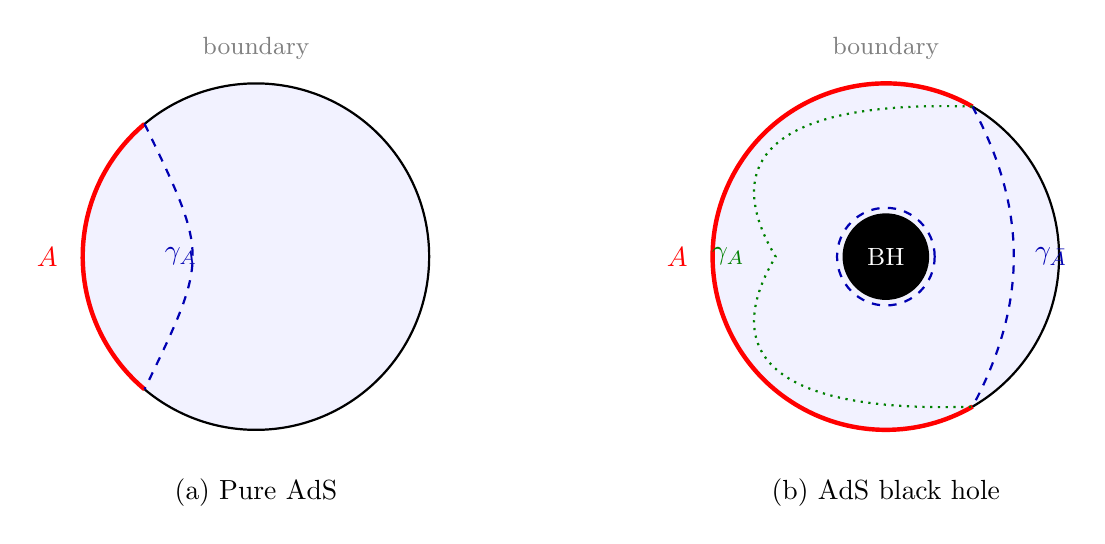
\begin{tikzpicture}[scale=1.0]
  \begin{scope}[xshift=-4cm]
    \fill[blue!5] (0,0) circle (2.2);
    \draw[thick] (0,0) circle (2.2);
    \draw[red, ultra thick] (130:2.2) arc (130:230:2.2);
    \node[red] at (180:2.65) {$A$};
    \draw[blue!70!black, thick, dashed]
      (130:2.2) .. controls (-0.6,0) .. (230:2.2);
    \node[blue!70!black] at (-0.95,0) {$\gamma_A$};
    \node at (0,-3.0) {(a) Pure AdS};
    \node[gray] at (0,2.65) {\small boundary};
  \end{scope}
  \begin{scope}[xshift=4cm]
    \fill[blue!5] (0,0) circle (2.2);
    \draw[thick] (0,0) circle (2.2);
    \fill[black] (0,0) circle (0.55);
    \node[white] at (0,0) {\small BH};
    \draw[red, ultra thick] (60:2.2) arc (60:300:2.2);
    \node[red] at (180:2.65) {$A$};
    \draw[blue!70!black, thick, dashed]
      (60:2.2) .. controls (1.8,0.6) and (1.8,-0.6) .. (300:2.2);
    \draw[green!50!black, thick, dotted]
      (60:2.2) .. controls (-1.8,2.0) and (-2.0,1.0) .. (-1.4,0)
      .. controls (-2.0,-1.0) and (-1.8,-2.0) .. (300:2.2);
    \draw[blue!70!black, thick, dashed] (0,0) circle (0.62);
    \node[blue!70!black] at (2.1,0) {$\gamma_{\bar A}$};
    \node[green!50!black] at (-2.0,0) {$\gamma_A$};
    \node at (0,-3.0) {(b) AdS black hole};
    \node[gray] at (0,2.65) {\small boundary};
  \end{scope}
\end{tikzpicture}
\end{adjustbox}
\caption{The Ryu--Takayanagi surface in two settings.
  (a)~In pure AdS, the minimal surface $\gamma_A$ homologous to
  boundary region~$A$ is a bulk geodesic connecting the endpoints of
  $\partial A$.  (b)~In a black hole background (the thermal state),
  a sufficiently large boundary region admits two candidates: a connected
  geodesic homologous to $A$ (dotted green), and the complementary geodesic
  together with the horizon (both dashed blue).
  The RT prescription selects the candidate
  with smaller total area.  When $A$ is the entire boundary in the
  thermal state, the homologous surface is the horizon itself, and
  the RT formula reduces to the Bekenstein--Hawking entropy.}
\label{fig04:rt_surface}
\end{figure}

\subsubsection*{Simple examples}

To build intuition, consider two cases (illustrated in
Figure~\ref{fig04:rt_surface}):

\paragraph{Pure AdS.}
The bulk geometry is ``empty'' anti-de Sitter space, dual to the
vacuum state of the CFT.  For a connected boundary interval~$A$ in
AdS$_3$/CFT$_2$, the minimal surface~$\gamma_{A}$ is a bulk
geodesic---the shortest curve connecting the two endpoints
of~$\partial A$ that dips into the interior.  A short interval has a
shallow geodesic (small area, small entropy); a longer interval has a
deeper geodesic (larger area, larger entropy).  This matches the
universal logarithmic scaling of entanglement entropy in a
two-dimensional CFT~\citep{calabresecardy2004}.

\paragraph{AdS with a black hole.}
Now consider a large black hole occupying the center of AdS.  For a
small boundary region~$A$, the minimal surface is still a geodesic
that barely enters the bulk.  But as~$A$ grows to cover most of the
boundary, a topological transition occurs: the minimal surface
``jumps'' to one that wraps around the black hole horizon.  At this
point the disconnected candidate gives
$S(A)\simeq S(\bar A)+A_{\mathrm{horizon}}/(4G_N)$ at leading order,
with the same ultraviolet regulator on both boundary entropies. For the
entire thermal system only the horizon contribution remains.

This topological transition---between two candidate surfaces---is a
recurring theme.  As we will see, a closely analogous transition
underlies the Page curve itself.

\subsubsection*{Scope and limitations}

The RT formula~\eqref{eq04:rt} applies to static geometries and
holographic CFTs at leading order in $1/G_N$ (equivalently, large
central charge).  Its covariant generalization to dynamical spacetimes
was given by Hubeny, Rangamani, and
Takayanagi~\citeyearpar{hubenyetal2007}, who replace the minimal surface
with an \emph{extremal} surface (one whose area is stationary under
small deformations).  We will refer to this covariant version as the
HRT formula.

Crucially, both RT and HRT are \emph{classical}: they compute the
leading-order entanglement entropy and neglect quantum corrections
(bulk entanglement, one-loop effects, etc.).  For many purposes this
is perfectly adequate.  But for the information paradox, it is not
enough. Bulk entropy can accumulate to the size of the area term over
the evaporation history, so a contribution subleading at fixed time can
participate in a leading competition at late times. This motivates the
generalized-entropy prescription described next.


\subsection{Quantum extremal surfaces: the upgrade}
\label{subsec04:qes}

\subsubsection*{The need for quantum corrections}

The RT formula computes entanglement entropy to leading order in
$1/G_N$.  In the holographic dictionary, $1/G_N$ plays the role of a
large parameter (analogous to $N^2$ in a gauge theory with $N$
colors), so the RT formula captures the ``classical'' or ``planar''
contribution.  But quantum effects in the bulk---loop corrections,
entanglement of bulk quantum fields---contribute at subleading order.
For a complete answer, one needs to include these corrections.

The importance of this for black holes is immediate.  The
Bekenstein--Hawking entropy $S_{\mathrm{BH}} =
A_{\mathrm{horizon}}/(4G_N)$ is an $O(1/G_N)$ quantity.  Hawking's
monotonically rising radiation entropy is also $O(1/G_N)$.  The
``error'' that leads to the information paradox is therefore a
leading-order effect.  Resolving it requires a formula that correctly
competes the leading area term against the growing bulk entropy.

The first step beyond the classical formula was taken by Faulkner,
Lewkowycz, and Maldacena~\citeyearpar{faulkneretal2013}, who computed
the leading quantum correction to holographic entanglement entropy:
the bulk entanglement entropy $S_{\mathrm{bulk}}$ of the quantum
fields, evaluated at the classical RT surface, is added to the area
term.  Engelhardt and Wall then promoted this one-loop correction to
a full prescription that extremizes the generalized entropy itself.

\subsubsection*{The Engelhardt--Wall prescription}

In 2015, Netta Engelhardt and Aron Wall proposed the \textbf{quantum
extremal surface} (QES) prescription~\citeyearpar{engelhardtwall2015}.  It
replaces the RT/HRT formula with:
\begin{equation}
\label{eq04:qes}
\boxed{
S(A) \;=\; \min_{\chi}\,\underset{\text{extremal}}{\mathrm{ext}}
\left[
  \frac{\mathrm{Area}(\chi)}{4\,G_{N}}
  \;+\; S_{\mathrm{bulk}}(\Sigma_{\chi})
\right]
}
\qquad\text{(QES prescription)}\,,
\end{equation}
where:
\begin{itemize}
\item $\chi$ is a codimension-two surface in the bulk, anchored to
  $\partial A$ on the boundary;
\item $\Sigma_{\chi}$ is the bulk region on a Cauchy slice between
  $\chi$ and the boundary region~$A$ (the homology region; its
  domain of dependence is the ``entanglement wedge'');
\item $S_{\mathrm{bulk}}(\Sigma_{\chi})$ is the von~Neumann entropy
  of the bulk quantum fields restricted to $\Sigma_{\chi}$;
\item ``ext'' means we find surfaces that \emph{extremize} the
  generalized entropy (area term plus bulk entropy), and ``min''
  selects the one with the smallest value among all extrema.
\end{itemize}

The two-step instruction---first extremize, then minimize---is
essential.  The functional
$S_{\mathrm{gen}}(\chi) = \mathrm{Area}(\chi)/(4G_N) +
S_{\mathrm{bulk}}(\Sigma_\chi)$
is called the \textbf{generalized entropy} of the surface~$\chi$.  In
general, there may be multiple surfaces at which
$S_{\mathrm{gen}}$ is stationary.  Each such surface is a quantum
extremal surface.  The prescription instructs us to pick the global
\emph{minimum} among these extrema---the one with the smallest
generalized entropy.

The area and bulk entropy require a common renormalization prescription;
the displayed formula uses Einstein gravity and suppresses higher-derivative
entropy terms. It is the usual semiclassical prescription. Particular
states and transitions can require refinements, including the leading
QES corrections of \citet{akerspenington2021}; see
Section~\ref{sec10:genus_corrections}.

When $S_{\mathrm{bulk}} = 0$ (no bulk entropy contribution), the QES
prescription reduces to HRT, or RT in a static setting: extremizing the area
alone recovers the minimal surface, and we are back to
Eq.~\eqref{eq04:rt}.

\subsubsection*{Multiple extrema and the phase transition}

The content of the QES prescription lies in the possibility of
\emph{multiple} quantum extremal surfaces for the same boundary
region.  This is where the resolution of the information paradox
emerges.

Consider computing the entanglement entropy of the Hawking radiation
emitted by an evaporating black hole.  In an appropriate holographic
setup (we will be more precise momentarily), the QES prescription
identifies two competing extremal surfaces:

\begin{enumerate}
\item \textbf{The ``empty'' surface} (trivial QES).  This surface is
  trivial in the sense that its area vanishes (or is negligible).  The
  generalized entropy is then dominated by
  $S_{\mathrm{bulk}}(\Sigma)$, which includes all the Hawking
  radiation.  This contribution grows monotonically as the black hole
  evaporates, tracking Hawking's original calculation.

\item \textbf{The ``island'' surface} (non-trivial QES).  This
  surface lies near the black hole horizon.  Its area term
  $\mathrm{Area}(\chi)/(4G_N)$ gives a contribution close to the
  Bekenstein--Hawking entropy, which \emph{decreases} as the black
  hole shrinks.  The bulk entropy term is now evaluated on a
  union of the radiation region and an interior region---the ``island''
  (Section~\ref{subsec04:island} below). Including partners of outgoing
  modes can lower the bulk entropy of this union.
\end{enumerate}

\begin{figure}[t]
\centering
\begin{adjustbox}{max width=\textwidth, center}
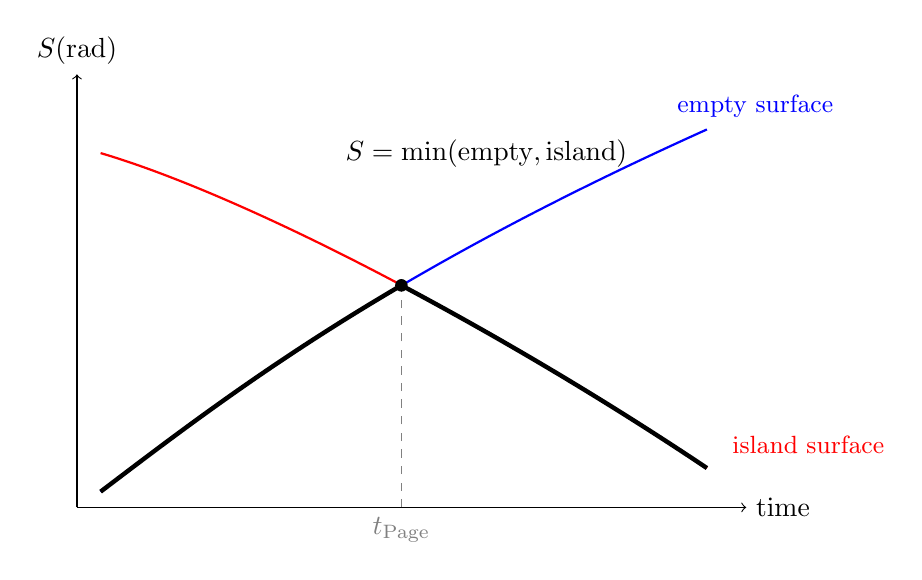
\begin{tikzpicture}[scale=1.0]
  \draw[->] (0,0) -- (8.5,0) node[right] {time};
  \draw[->] (0,0) -- (0,5.5) node[above] {$S(\mathrm{rad})$};
  \draw[blue, thick]
    (0.3,0.2) .. controls (2,1.5) and (4,3.0) .. (8,4.8);
  \node[blue, right] at (7.5,5.1) {\small empty surface};
  \draw[red, thick]
    (0.3,4.5) .. controls (2,4.0) and (5,2.5) .. (8,0.5);
  \node[red, right] at (8.2,0.8) {\small island surface};
  \draw[black, ultra thick]
    (0.30,0.20) .. controls (1.34,0.99) and (2.48,1.86) .. (4.12,2.82);
  \draw[black, ultra thick]
    (4.12,2.82) .. controls (5.34,2.17) and (6.67,1.39) .. (8.00,0.50);
  \draw[dashed, gray] (4.12,0) -- (4.12,2.82);
  \node[below, gray] at (4.12,0) {$t_{\mathrm{Page}}$};
  \fill (4.12,2.82) circle (0.08);
  \node at (5.2,4.5) {$S = \min(\text{empty}, \text{island})$};
\end{tikzpicture}
\end{adjustbox}
\caption{Competition between the two quantum extremal surfaces.
  The blue (empty surface) curve tracks Hawking's monotonically
  growing result.  The red (island surface) curve starts at the
  initial Bekenstein--Hawking entropy and decreases as the black
  hole evaporates.  The QES prescription instructs us to take the
  global minimum (bold black curve), which transitions from the
  empty surface to the island surface at the \emph{Page time}.
  The resulting curve is the Page curve.}
\label{fig04:qes_competition}
\end{figure}

The QES prescription says: take the minimum.  At early times, the
empty surface has lower generalized entropy (the radiation entropy is
still small), so it wins.  At late times, the island surface has lower
generalized entropy (the black hole has shrunk), so it wins.  The
crossover defines the \textbf{Page time} $t_{\mathrm{Page}}$, and the
envelope of the two curves is precisely the Page curve
(Figure~\ref{fig04:qes_competition}).

Schematically:
\begin{equation}
\label{eq04:page_curve_qes}
S(\mathrm{rad}) \;=\;
\begin{cases}
  S_{\mathrm{bulk}}(\mathrm{rad}) & t < t_{\mathrm{Page}}
  \quad\text{(empty surface)}\,,\\[6pt]
  \dfrac{A_{\mathrm{horizon}}}{4G_N} + \ldots & t > t_{\mathrm{Page}}
  \quad\text{(island surface)}\,.
\end{cases}
\end{equation}
Before the Page time, the entropy grows (tracking Hawking's result).
After the Page time, it decreases (tracking the shrinking horizon).
The result is $S(\mathrm{rad}) \approx
\min\bigl(S_{\mathrm{thermo}},\, S_{\mathrm{BH}}\bigr)$, where
$S_{\mathrm{thermo}}$ denotes the thermodynamic (coarse-grained)
entropy of the radiation emitted so far and $S_{\mathrm{BH}}$ the
instantaneous Bekenstein--Hawking entropy of the black hole---which
is exactly the Page curve.

This is the central result:
\begin{quote}
\emph{The quantum extremal surface prescription, applied to an
evaporating black hole, produces the Page curve.  This was
demonstrated independently in~2019 by
Penington~\citeyearpar{penington2020} and by Almheiri, Engelhardt,
Marolf, and Maxfield~\citeyearpar{almheirietal2019}.}
\end{quote}

This calculation gives a geometric entropy turnover in the specified
semiclassical models. It goes beyond the original disconnected saddle
without supplying a complete microscopic evaporation channel.
The distinction between entropy and channel data is developed in
Section~\ref{sec14:equilibrium_evaporation}.

\subsection{The island rule}
\label{subsec04:island}

The QES prescription described above can be repackaged into a
particularly intuitive form called the \textbf{island
rule}~\citep{almheirietal2020islands}.  This formulation makes
explicit the role of the ``island''---a region of the black hole
interior that, after the Page time, is ``owned by'' the radiation.

\subsubsection*{Setup}

Consider a black hole that is evaporating into a region we call the
``radiation reservoir'' (or simply ``rad'').  We want to compute
$S(\mathrm{rad})$, the entanglement entropy of the radiation.  In a
holographic setup, the radiation lives on a non-gravitational bath
coupled to the gravitational region containing the black hole.

\subsubsection*{The formula}

The island rule states:
\begin{equation}
\label{eq04:island_rule}
\boxed{
S(\mathrm{rad}) \;=\; \min_{I}\,\underset{\text{extremal}}{\mathrm{ext}}
\left[
  \frac{\mathrm{Area}(\partial I)}{4\,G_{N}}
  \;+\; S_{\mathrm{bulk}}(\mathrm{rad} \cup I)
\right]
}
\qquad\text{(island rule)}\,.
\end{equation}
Here:
\begin{itemize}
\item $I$ is a spatial region in the gravitational sector (the
  ``island'').  The island may be empty ($I = \varnothing$) or
  non-empty.
\item $\partial I$ is the boundary of the island.  When $I =
  \varnothing$, $\mathrm{Area}(\partial I) = 0$.
\item $S_{\mathrm{bulk}}(\mathrm{rad}\cup I)$ is the von~Neumann
  entropy of the bulk quantum fields on the union of the radiation
  region and the island.
\item The optimization is over all possible islands, including the
  trivial one.
\end{itemize}

\begin{figure}[t]
\centering
\begin{adjustbox}{max width=\textwidth, center}
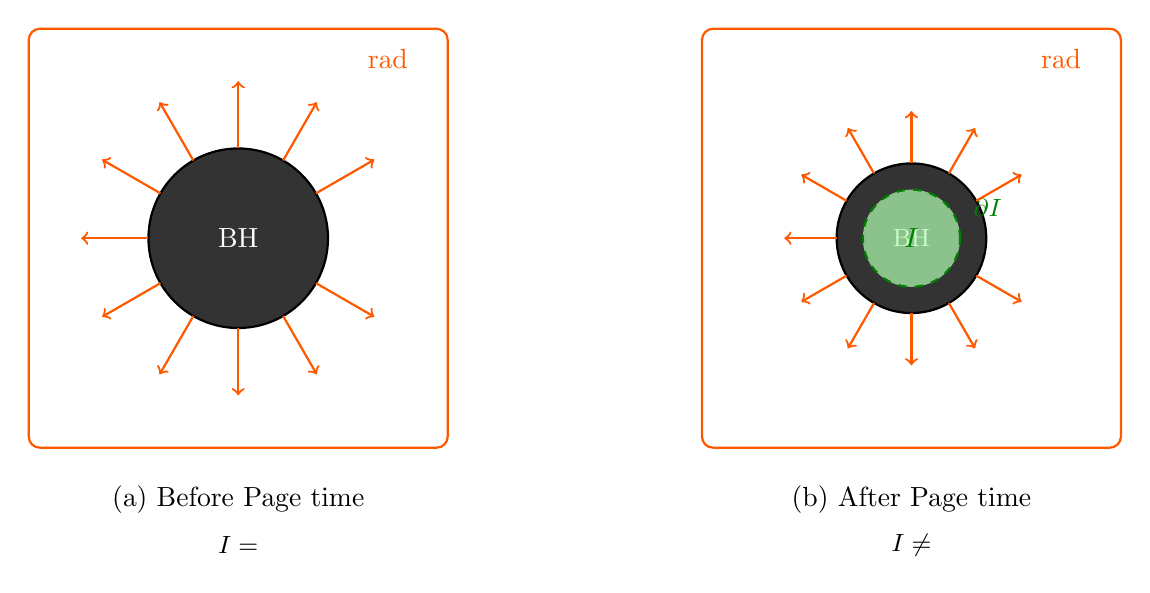
\begin{tikzpicture}[scale=0.95]
  \begin{scope}[xshift=-4.5cm]
    \fill[black!80] (0,0) circle (1.2);
    \node[white] at (0,0) {BH};
    \draw[thick] (0,0) circle (1.2);
    \foreach \a in {30,60,...,330} {
      \draw[->, orange!70!red, thick] (\a:1.2) -- (\a:2.1);
    }
    \draw[orange!70!red, thick, rounded corners]
      (-2.8,-2.8) rectangle (2.8,2.8);
    \node[orange!70!red] at (2.0,2.4) {rad};
    \node at (0,-3.5) {(a) Before Page time};
    \node at (0,-4.1) {\small $I = \varnothing$};
  \end{scope}
  \begin{scope}[xshift=4.5cm]
    \fill[black!80] (0,0) circle (1.0);
    \node[white] at (0,0.0) {\small BH};
    \draw[thick] (0,0) circle (1.0);
    \fill[green!30, opacity=0.7] (0,0) circle (0.65);
    \draw[green!50!black, thick, dashed] (0,0) circle (0.65);
    \node[green!50!black] at (0,0) {$I$};
    \node[green!50!black, right] at (0.7,0.4) {\small $\partial I$};
    \foreach \a in {30,60,...,330} {
      \draw[->, orange!70!red, thick] (\a:1.0) -- (\a:1.7);
    }
    \draw[orange!70!red, thick, rounded corners]
      (-2.8,-2.8) rectangle (2.8,2.8);
    \node[orange!70!red] at (2.0,2.4) {rad};
    \node at (0,-3.5) {(b) After Page time};
    \node at (0,-4.1) {\small $I \neq \varnothing$};
  \end{scope}
\end{tikzpicture}
\end{adjustbox}
\caption{The island rule illustrated schematically.
  (a)~Before the Page time, the island is empty ($I = \varnothing$).
  The entropy of the radiation is computed from the bulk entropy of
  the radiation alone, which grows monotonically.
  (b)~After the Page time, a non-trivial island~$I$ appears inside
  the black hole.  The radiation entropy is now computed from the
  generalized entropy: the area of $\partial I$ (the QES, shown
  dashed) plus the bulk entropy of $\mathrm{rad} \cup I$.  Because
  the island ``absorbs'' the interior partners of the Hawking quanta,
  the bulk entropy term is reduced, and the total entropy decreases.}
\label{fig04:island}
\end{figure}

\subsubsection*{Two phases}

The island rule identifies two competing saddle points:

\paragraph{No-island phase ($I = \varnothing$).}
When the island is empty, $\partial I$ is also empty, and the formula
reduces to
\begin{equation}
\label{eq04:no_island}
S(\mathrm{rad}) = S_{\mathrm{bulk}}(\mathrm{rad})\,.
\end{equation}
This is just the entropy of the Hawking radiation computed in the
semiclassical approximation---Hawking's original, monotonically
growing answer.

\paragraph{Island phase ($I \neq \varnothing$).}
When a non-trivial island exists, it typically sits just inside the
black hole horizon (Figure~\ref{fig04:island}b).  Its boundary
$\partial I$ is the quantum extremal surface, and the generalized
entropy is approximately
\begin{equation}
\label{eq04:island_phase}
S(\mathrm{rad}) \;\approx\;
\frac{A_{\mathrm{horizon}}}{4\,G_{N}}
\;+\; S_{\mathrm{bulk}}(\mathrm{rad} \cup I)\,.
\end{equation}
The bulk entropy of $\mathrm{rad}\cup I$ is much smaller than
$S_{\mathrm{bulk}}(\mathrm{rad})$ alone, because including the
island brings in the interior partners of the Hawking quanta.
These partners are entangled with the radiation, so including
them in the same subsystem \emph{reduces} the entanglement
entropy.  The dominant contribution is the area term, which
decreases as the black hole evaporates.

The island rule selects whichever phase has lower entropy.  Before
the Page time, the no-island phase wins.  After the Page time, the
island phase wins.  The result is the Page curve.

\subsubsection*{Interpretation: what the island means}

The appearance of an island has a striking interpretation.  After the
Page time, a spatial region~$I$ inside the black hole is
\emph{encoded in the radiation}.  In the language of quantum error
correction (which underlies the modern understanding of holography),
the island is part of the ``entanglement wedge'' of the radiation:
an observer with access to the radiation can, in principle,
reconstruct operators acting on the island.

This is deeply counterintuitive.  In the evaporating case the island
lies behind the horizon, spacelike separated from the late-time
radiation region it purifies (in eternal-black-hole-plus-bath setups,
islands can even extend outside the horizon).  Yet the island rule
tells us that, after the Page time, this interior region is
reconstructable from the radiation.  This describes the encoding of a bulk operator algebra, not a local
signal propagating outward across a classical event horizon.

\subsubsection*{A caveat: formula, not mechanism}

In its applicable regime the island rule computes semiclassical entropy
and identifies an entanglement wedge associated with the radiation.
Entanglement-wedge reconstruction gives operator-algebraic meaning to this
region, conditional on the chosen semiclassical code subspace. The entropy
formula alone does not specify a state-independent decoder or the entire
dynamical process that accomplishes the encoding. Replica wormholes and
entropy statistics supply additional calculations, developed in
Sections~\ref{sec05:path_integral} and \ref{sec06:replica_wormholes}.

\subsection{What was achieved and what remains open}
\label{subsec04:achieved}

Let us take stock.

\subsubsection*{The achievement}

The QES prescription and the island rule represent a genuine
breakthrough.  For the first time since Hawking's 1975
paper~\citep{hawking1975}, there exists a gravitational calculation
that produces the Page curve:

\begin{enumerate}
\item The \textbf{Ryu--Takayanagi formula}~\citep{ryutakayanagi2006}
  established that entanglement entropy is computed by the area of a
  minimal surface in the bulk.

\item The \textbf{quantum extremal surface
  prescription}~\citep{engelhardtwall2015} upgraded this to include
  bulk quantum corrections, introducing the generalized entropy.

\item \textbf{Penington}~\citeyearpar{penington2020} and \textbf{Almheiri et
  al.}~\citeyearpar{almheirietal2019} showed that the QES prescription,
  applied to an evaporating black hole, produces the Page
  curve.  The key is the exchange of dominance between two
  quantum extremal surfaces at the Page time.

\item The \textbf{island rule}~\citep{almheirietal2020islands}
  repackaged this into a formula directly for the radiation entropy,
  making the role of the island explicit.
\end{enumerate}

In the stated holographic and bath-coupled models, these results derive
the entropy turnover from a gravitational prescription. Reconstructing
interior observables and identifying the full evaporation channel require
additional information.

\subsubsection*{What remains open}

Despite this progress, several deep questions remain:

\begin{enumerate}
\item \textbf{How does information escape?}  The island rule tells us
  \emph{that} information is encoded in the radiation, but not
  \emph{how} it gets there.  What is the physical mechanism at the
  horizon?  Does an infalling observer notice anything?  These
  questions remain open.

\item \textbf{Single theory vs.\ ensemble.}  The gravitational path
  integral in JT gravity has an ensemble interpretation, whereas a fixed
  holographic CFT is a single theory. One must identify which quantities
  are averaged in a particular calculation; QES does not itself imply
  averaging over Hamiltonians.  The relationship between single
  realizations and ensemble averages is a subject of active
  investigation~\citep{saadetal2019, wuebben2026paper3}.

\item \textbf{What happens at the horizon?}  Different proposals
  exist: firewalls~\citep{ampsetal2013}, fuzzballs~\citep{mathur2005},
  smooth horizons with subtle encoding~\citep{papadodimasraju2013},
  ER=EPR~\citep{maldacenasusskind2013}.  The island rule
  does not by itself determine which horizon description applies. Whether
  two specified models yield the same observables must be calculated.

\item \textbf{Detailed transition structure.}  The QES prescription
  predicts a sharp phase transition at the Page time: a discrete
  swap between two saddle points. For a finite-dimensional density matrix
  varying continuously with a parameter, entropy is continuous, although
  differentiability requires additional conditions.  What controls
  the width and shape of this transition?  What are the corrections
  to the sharp-swap approximation?
\end{enumerate}

The second and fourth questions---the ensemble structure of the
gravitational path integral and the detailed transition
structure---are precisely the subject of the companion
papers~\citep{wuebben2026paper1, wuebben2026paper2, wuebben2026paper3}
and of the remainder of this tutorial: Papers~I and~II develop the
detailed structure of the Page transition, while Paper~III takes up
the ensemble and microscopic-ambiguity questions.  The gravitational
path integral, replica wormholes, and
free probability theory will provide the tools to resolve the
transition and go beyond the leading-order Page curve.  We turn to
these tools in Part~II.


\part{The Gravitational Path Integral and Replica Wormholes}

\section{The Gravitational Path Integral}\label{sec05:path_integral}

The previous sections assembled the physical ingredients: quantum mechanics,
black holes, Hawking radiation, and the holographic principle.  We now turn to
the \emph{computational} framework that makes the Page curve derivable within
semiclassical gravity: the gravitational path integral.  This is the tool that
will, in the next section, produce replica wormholes and the leading
entropy turnover in specified models.

The gravitational path integral is simultaneously one of the deepest and one of
the most poorly defined objects in theoretical physics.  It is deep because it
encodes the quantum-mechanical sum over all possible spacetimes --- not just over
field configurations on a fixed background, but over the geometries themselves.
It is poorly defined because, unlike the path integral for a scalar field, a general nonperturbative definition for the gravitational theories
considered here is not available.  Nevertheless, when used with
appropriate care --- principally through the saddle-point approximation and its
systematic corrections --- it produces results of considerable power and precision.

This section develops the gravitational path integral in three stages.  We begin
with the basic idea of the path integral and explain what changes when the
dynamical variable is the metric itself.  We then introduce the genus expansion,
which organizes two-dimensional topologies as a perturbative series. We
then distinguish its relation to matrix integrals from the particular
contraction combinatorics of a random-state model.  Finally, we
explain the Wick rotation to Euclidean signature and the thermal interpretation
that makes the black hole path integral tractable.


\subsection{Path integrals: the basic idea}\label{subsec05:basic_idea}

\subsubsection*{Feynman's sum over histories}

The path integral formulation of quantum mechanics, due to
\citet{feynman1948}, recasts the transition amplitude between two states as a sum
over all possible histories connecting them.  For a particle moving from position
$q_i$ at time $t_i$ to position $q_f$ at time $t_f$, the amplitude is
\begin{equation}\label{eq05:particle_path_integral}
  \langle q_f, t_f \,|\, q_i, t_i \rangle
  \;=\; \int \mathcal{D}q(t)\; e^{\,i\,S[q]/\hbar}\,,
\end{equation}
where $S[q] = \int_{t_i}^{t_f} L(q,\dot{q})\,dt$ is the classical action and
the integral runs over \emph{all} paths $q(t)$ with the specified boundary
conditions.  Each path contributes with a phase $e^{iS/\hbar}$; the classical
path --- the one that extremizes $S$ --- dominates because nearby paths
constructively interfere, while paths far from the classical trajectory
contribute rapidly oscillating phases that cancel.

The same logic extends to quantum field theory.  For a scalar field $\phi$ on a
fixed spacetime background, the generating functional (partition function) is
\begin{equation}\label{eq05:qft_path_integral}
  Z \;=\; \int \mathcal{D}\phi\; e^{\,i\,S[\phi]/\hbar}\,.
\end{equation}
This is the starting point for all perturbative calculations in the Standard
Model and in quantum field theory on curved spacetime.

\subsubsection*{Gravity: summing over geometries}

The gravitational path integral makes a conceptual leap: it promotes the
\emph{spacetime geometry itself} to a dynamical variable.  Rather than
integrating over field configurations on a fixed background, we integrate over
all metrics $g_{\mu\nu}$ on a manifold $\mathcal{M}$, weighted by the
Einstein--Hilbert action:
\begin{equation}\label{eq05:grav_path_integral_lorentzian}
  Z \;=\; \int \mathcal{D}g_{\mu\nu}\; e^{\,i\,S_{\mathrm{EH}}[g]/\hbar}\,,
  \qquad
  S_{\mathrm{EH}} = \frac{1}{16\pi G_N}\int_{\mathcal{M}} d^{d+1}x\,\sqrt{-g}\;
  \bigl(R - 2\Lambda\bigr) + S_{\mathrm{bdy}}\,,
\end{equation}
where $R$ is the Ricci scalar, $\Lambda$ is the cosmological constant,
$G_N$ is Newton's constant, and $S_{\mathrm{bdy}}$ denotes the
Gibbons--Hawking--York boundary term \citep{gibbonshawking1977, york1972} needed
to make the variational problem well-posed on manifolds with boundary.

Three features distinguish the gravitational path integral from its field-theory
counterpart:

\begin{enumerate}
  \item \textbf{The integration variable is the geometry.}  In ordinary quantum
    field theory, the background spacetime is fixed and the path integral sums
    over matter field configurations.  In quantum gravity, the metric is itself
    integrated over.  There is no fixed stage on which the drama unfolds; the
    stage is part of the show.

  \item \textbf{The sum includes different topologies.}  In particle physics, the
    path integral for a scalar field sums over all field configurations on
    $\mathbb{R}^{3,1}$.  The topology of spacetime is fixed.  In gravity, we must
    also sum over manifolds of different topology --- spacetimes with handles,
    wormholes, and other non-trivial topological features.  This ``sum over
    topologies'' has no analogue in the Standard Model and is the source of much
    of the richness (and difficulty) of quantum gravity.

  \item \textbf{There is no known rigorous measure.}  The measure
    $\mathcal{D}g_{\mu\nu}$ must account for the gauge redundancy of
    diffeomorphisms, the conformal factor problem (the Euclidean action is
    unbounded below for conformal deformations), and the absence of a background
    with respect to which ``small fluctuations'' can be defined.  These problems
    are not merely technical; they reflect the deep conceptual challenge of
    defining quantum gravity non-perturbatively.
\end{enumerate}

Despite these difficulties, the \textbf{saddle-point approximation} gives
controlled calculations in suitable regimes, once boundary conditions,
gauge fixing, and an integration contour have been specified.

\subsubsection*{The saddle-point approximation}

The saddle-point (or stationary-phase) approximation to a path integral retains
only the contributions from configurations that extremize the action --- i.e., the
classical solutions --- together with Gaussian fluctuations around them.
Schematically:
\begin{equation}\label{eq05:saddle_point}
  Z \;\approx\; \sum_{\text{saddles}\;\sigma}\;
  e^{\,-I[\sigma]}\;\cdot\;
  Z^{(1)}_{\sigma}\;\cdot\;
  \bigl(1 + O(G_N)\bigr)\,,
\end{equation}
where $I[\sigma]$ is the on-shell Euclidean action of the saddle $\sigma$ (we
explain the Euclidean formulation in Section~\ref{subsec05:euclidean}),
$Z^{(1)}_\sigma$ is the one-loop determinant from quadratic fluctuations around
the saddle, and the remaining corrections are organized as a perturbative
expansion in $G_N$.

The sum in Eq.~\eqref{eq05:saddle_point} runs over saddles compatible
with the boundary conditions and the integration contour.  This is a crucial point: the gravitational path integral
is not dominated by a single geometry, but by a \emph{sum} over geometries,
each weighted by $e^{-I}$.  When there are multiple saddles, the one with the
smallest action dominates, but the others contribute and can become important as
external parameters (such as the temperature or the age of the black hole) are
varied.  Phase transitions occur precisely when the dominant saddle changes ---
the Hawking--Page transition \citep{hawkingpage1983} between thermal AdS and the
AdS black hole being the classic example.

This is a semiclassical expansion, not a general nonperturbative
definition. Away from degeneracies a dominant saddle can control the answer;
near a transition several saddles can contribute comparably. In JT gravity
the topological entropy $S_0$ separately controls the cost of handles, as
explained below.

\begin{figure}[t]
\centering
\begin{adjustbox}{max width=\textwidth, center}
\begin{tikzpicture}[scale=1.0]
  \draw[thick, domain=-3.5:3.0, smooth, samples=100]
    plot (\x, {0.08*(\x+2)*(\x+2)*(\x-1.5)*(\x-1.5) - 0.5});
  \filldraw[blue] (-2, -0.5) circle (2.5pt) node[above=5pt]
    {saddle $\sigma_1$};
  \filldraw[red] (1.5, -0.5) circle (2.5pt) node[above=5pt]
    {saddle $\sigma_2$};
  \draw[->] (-4, -1.5) -- (4, -1.5) node[right] {field space};
  \draw[->] (-4, -1.5) -- (-4, 3) node[above] {$I[g]$};
  \draw[blue, dashed, <->] (-2.8, 0.3) -- (-1.2, 0.3)
    node[midway, above] {\small $Z^{(1)}_{\sigma_1}$};
  \draw[red, dashed, <->] (0.7, 0.3) -- (2.3, 0.3)
    node[midway, above] {\small $Z^{(1)}_{\sigma_2}$};
\end{tikzpicture}
\end{adjustbox}
\caption{Schematic illustration of the saddle-point approximation.  The
gravitational path integral receives its dominant contributions from classical
solutions (saddle points) of the Euclidean action.  Gaussian fluctuations around
each saddle produce the one-loop determinant $Z^{(1)}_\sigma$.  The full answer
is a sum over all saddles, weighted by $e^{-I[\sigma]}$.}\label{fig05:saddle_point}
\end{figure}


\subsection{The genus expansion}\label{subsec05:genus_expansion}

The sum over topologies in the gravitational path integral admits a natural
perturbative organization: the \textbf{genus expansion}.  This expansion is most
transparent in two-dimensional gravity, where orientable surfaces have
a simple classification. Higher-dimensional topology does not admit the
same general organization by one genus parameter.

\subsubsection*{Topology of surfaces}

A closed, connected, orientable two-dimensional surface is completely
characterized (up to homeomorphism) by a single integer: its \textbf{genus} $g$,
the number of handles.  The genus-zero surface is the sphere $S^2$; genus one is
the torus $T^2$; genus two is a ``pretzel'' with two handles; and so on
(Figure~\ref{fig05:genus_surfaces}).

The topological invariant that appears naturally in the gravitational action is
the \textbf{Euler characteristic}:
\begin{equation}\label{eq05:euler_characteristic}
  \chi \;=\; 2 - 2g\,.
\end{equation}
For the sphere $\chi = 2$, for the torus $\chi = 0$, and for higher-genus
surfaces $\chi < 0$.  The Gauss--Bonnet theorem relates $\chi$ to the integral
of the scalar curvature:
\begin{equation}\label{eq05:gauss_bonnet}
  \frac{1}{4\pi}\int_{\mathcal{M}} d^2x\,\sqrt{g}\; R
  \;=\; \chi(\mathcal{M}) \;=\; 2 - 2g\,.
\end{equation}
This is a topological invariant: it does not depend on the metric, only on the
topology of the surface.

\begin{figure}[t]
\centering
\begin{adjustbox}{max width=\textwidth, center}
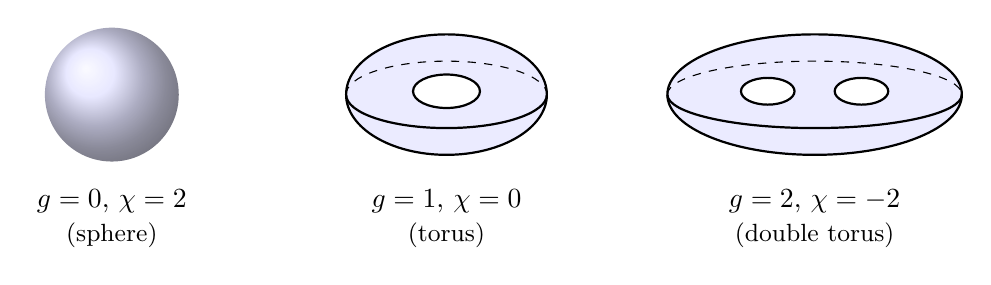
\begin{tikzpicture}[scale=0.85]
  \begin{scope}[xshift=-5cm]
    \shade[ball color=blue!15!white, opacity=0.8] (0,0) circle (1.0);
    \node at (0,-1.6) {$g=0$, $\chi=2$};
    \node at (0,-2.1) {\small (sphere)};
  \end{scope}
  \begin{scope}[xshift=0cm]
    \draw[thick, fill=blue!8!white]
      (0,0) ellipse (1.5 and 0.9);
    \draw[thick, fill=white]
      (0,0.05) ellipse (0.5 and 0.25);
    \draw[thick] (-1.5,0) arc (180:360:1.5 and 0.5);
    \draw[dashed, thin] (-1.5,0) arc (180:0:1.5 and 0.5);
    \node at (0,-1.6) {$g=1$, $\chi=0$};
    \node at (0,-2.1) {\small (torus)};
  \end{scope}
  \begin{scope}[xshift=5.5cm]
    \draw[thick, fill=blue!8!white]
      (0,0) ellipse (2.2 and 0.9);
    \draw[thick, fill=white]
      (-0.7,0.05) ellipse (0.4 and 0.2);
    \draw[thick, fill=white]
      (0.7,0.05) ellipse (0.4 and 0.2);
    \draw[thick] (-2.2,0) arc (180:360:2.2 and 0.5);
    \draw[dashed, thin] (-2.2,0) arc (180:0:2.2 and 0.5);
    \node at (0,-1.6) {$g=2$, $\chi=-2$};
    \node at (0,-2.1) {\small (double torus)};
  \end{scope}
\end{tikzpicture}
\end{adjustbox}
\caption{Orientable surfaces classified by genus $g$.  The genus counts the
number of handles: the sphere has none, the torus has one, and the double torus
has two.  The Euler characteristic $\chi = 2 - 2g$ decreases with increasing
genus.}\label{fig05:genus_surfaces}
\end{figure}

\subsubsection*{The genus expansion in JT gravity}

Jackiw--Teitelboim (JT) gravity \citep{jackiw1985, teitelboim1983} is a
two-dimensional theory of gravity that serves as a powerful toy model
for near-extremal black holes \citep{maldacena2016}; see
\citet{mertensturiaci2023} for a comprehensive review.  Its action is
\begin{equation}\label{eq05:jt_action}
  I_{\mathrm{JT}} \;=\; -S_0\,\chi(\mathcal{M})
  \;-\; \frac{1}{2}\int_{\mathcal{M}} d^2x\,\sqrt{g}\;\phi\,(R+2)
  \;-\; \int_{\partial\mathcal{M}} du\,\sqrt{h}\;\phi\,(K-1)\,,
\end{equation}
where $\phi$ is the dilaton field, $K$ is the extrinsic curvature of the
boundary, and $S_0$ is a topological coupling --- the extremal entropy of the
black hole.

The crucial feature is the topological term $-S_0\,\chi$: each topology enters
the path integral with a weight $e^{\,S_0\,\chi}$.  (For a surface with $n$
boundaries the Euler characteristic is $\chi = 2-2g-n$ rather than $2-2g$, so,
for example, the one-boundary disk carries a factor $e^{S_0}$; since adding a
handle lowers $\chi$ by two whatever the number of boundaries.) For a
connected amplitude with a fixed number $b$ of boundaries,
\begin{equation}\label{eq05:genus_expansion}
 Z_{\mathrm{conn},b}(\beta_1,\ldots,\beta_b)
 \sim \sum_{g\geq0} e^{(2-2g-b)S_0}
 Z_{g,b}(\beta_1,\ldots,\beta_b).
\end{equation}
Here $Z_{g,b}$ is the amplitude with the topological weight removed. Thus
\begin{equation}\label{eq05:genus_suppression}
 \frac{e^{(2-2(g+1)-b)S_0}Z_{g+1,b}}
      {e^{(2-2g-b)S_0}Z_{g,b}}
 =e^{-2S_0}\frac{Z_{g+1,b}}{Z_{g,b}}.
\end{equation}
At fixed genus and suitable fixed boundary parameters, large $S_0$
suppresses additional handles. The coefficients still matter: their
growth makes this an asymptotic series, and other limits can compensate
the topological suppression. A one-loop determinant on the disk is a
correction at fixed topology; it does not add a handle.

\subsubsection*{Analogy with matrix models and large $N$}

The structure of Eq.~\eqref{eq05:genus_expansion} is identical to the
topological expansion of matrix integrals \citep{thooft1974}.  In a Hermitian
matrix model with $N \times N$ matrices, Feynman diagrams can be drawn on
surfaces of genus $g$, and the partition function admits the expansion
\begin{equation}\label{eq05:matrix_genus}
  \ln Z_{\text{matrix}} \;=\; \sum_{g=0}^{\infty}\; N^{2-2g}\; F_g\,,
\end{equation}
with the identification $N^2 \leftrightarrow e^{2S_0}$.  This is not a
coincidence.  \citet{saadetal2019} showed, order by order in the genus
expansion, that the perturbative series of JT gravity coincides with that of a
specific double-scaled random matrix ensemble; the exact nonperturbative
duality between the gravitational path integral and random matrix theory
remains conjectural.

The correspondence relates the JT genus expansion to a matrix-integral
expansion. A separate random-state problem describes the reduced density
matrix of a bipartite Gaussian state. Its Wick contractions can also be
drawn as ribbon graphs. At leading order, the surviving contractions are
indexed by non-crossing partitions \citep{speicher1994}. This is the
connection used in Sections~\ref{sec06:replica_wormholes} and
\ref{sec07:free_probability}.

\subsubsection*{Planar contractions and non-crossing partitions}

A ribbon graph records a cyclic order of edges at each vertex. Its faces
supply factors of matrix dimension, and Euler's relation determines the
power of that dimension. For the flat-weight Wishart moment problem,
maximizing the number of faces selects permutations associated with
non-crossing partitions. Their weights give the Marchenko--Pastur law.
Changing the spectral weights changes the moment sum even when the
contractions remain planar. In the gravitational problem these weights
encode the preparation and disk amplitudes
\citep{pssyetal2022,wang2023,chengetal2024}.

\begin{center}
\begin{adjustbox}{max width=\textwidth,center}
\begin{tabular}{lll}
\toprule
\textbf{Calculation} & \textbf{Organization} & \textbf{Additional input} \\
\midrule
Connected JT amplitudes & Genus and boundaries & $Z_{g,b}(\beta_1,\ldots)$ \\
Gaussian matrix moments & Wick ribbon graphs & Matrix dimensions and covariance \\
Flat-weight planar moments & Non-crossing partitions & Uniform covariance \\
Weighted planar moments & Free moment expansions & Spectral weights \\
\bottomrule
\end{tabular}
\end{adjustbox}
\end{center}

The shared combinatorial language is useful, but these are different
amplitudes. In particular, a finite Wick sum at fixed moment order is not
the complete JT sum over all handles. Section~\ref{sec10:genus_corrections}
returns to the distinction when discussing finite-size corrections.

\subsubsection*{Higher dimensions}

In dimensions $d > 2$, the classification of manifolds by a single integer like
the genus is no longer available --- the homeomorphism problem for closed
four-manifolds, for example, is algorithmically undecidable
\citep{markov1958}.  There is no general rule that a more complicated higher-dimensional
topology has a larger Einstein action or an extra factor $e^{-1/G_N}$.
The relative weights must be found from the admissible saddles and their
actions in the theory and ensemble under consideration.

In the context of the replica trick and entropy calculations (developed in the
next section), the relevant topologies in any dimension are ``replica
wormholes'' --- saddle points that connect different replicas of the spacetime.
This Euclidean route to entanglement entropy is the same one by which the
Ryu--Takayanagi formula itself is derived from the gravitational path integral
\citep{lewkowyczmaldacena2013}.
The structure of the calculation, and the competition between connected and
disconnected saddles, is qualitatively the same as in two dimensions, even though
the detailed geometry is much richer.


\subsection{Euclidean vs.\ Lorentzian: why we go to Euclidean signature}
\label{subsec05:euclidean}

Throughout this section we have written the gravitational path integral in
Euclidean signature, with a weight $e^{-I}$ rather than $e^{iS}$.  This
subsection explains why.

\subsubsection*{Wick rotation}

The passage from Lorentzian to Euclidean signature is achieved by the
\textbf{Wick rotation}: the analytic continuation of the time coordinate to
imaginary values,
\begin{equation}\label{eq05:wick_rotation}
  t \;\longrightarrow\; -i\tau\,,
  \qquad
  ds^2 = -dt^2 + d\vec{x}^{\,2}
  \;\longrightarrow\;
  ds^2_E = d\tau^2 + d\vec{x}^{\,2}\,.
\end{equation}
Under this rotation, the Lorentzian action $S$ becomes $iI$ where $I$ is the
Euclidean action, and the oscillatory weight $e^{iS/\hbar}$ becomes the
damped weight $e^{-I/\hbar}$:
\begin{equation}\label{eq05:wick_action}
  e^{\,i\,S_{\mathrm{Lor}}/\hbar}
  \;\longrightarrow\;
  e^{-I_{\mathrm{Eucl}}/\hbar}\,.
\end{equation}
For a stable bosonic action the Euclidean weight can improve convergence
and makes steepest-descent estimates transparent. This improvement does
not automatically hold in gravity, where the integration contour and
negative modes require separate treatment.  This is in contrast to the Lorentzian integral, where the
oscillatory phase $e^{iS}$ does not damp and the integral requires careful
definition through $i\epsilon$ prescriptions.

In quantum field theory on flat space, the Wick rotation is a standard and
well-understood procedure, related, under the appropriate positivity and regularity axioms, to
Lorentzian correlation functions by Osterwalder--Schrader reconstruction \citep{osterwalderschrader1973, osterwalderschrader1975}.  In gravity,
the situation is more subtle.  The Euclidean action for gravity is not bounded
below (the conformal factor problem), and not every Euclidean geometry has a
Lorentzian continuation.  Nevertheless, the Euclidean approach, used judiciously
at the level of saddle-point geometries, has proven highly successful.

\subsubsection*{Thermal interpretation: periodicity and temperature}

The most important consequence of the Wick rotation for black hole physics is
the connection between \textbf{Euclidean time periodicity and temperature}.

Consider a quantum system at inverse temperature $\beta = 1/T$.  Its thermal
partition function is
\begin{equation}\label{eq05:thermal_partition}
  Z(\beta) \;=\; \operatorname{Tr}\bigl(e^{-\beta H}\bigr)\,.
\end{equation}
In the path-integral representation, this trace is computed by evolving in
Euclidean time $\tau$ from $0$ to $\beta$ with \textbf{periodic boundary
conditions}: the field configurations at $\tau = 0$ and $\tau = \beta$ are
identified for bosonic variables; thermal fermions instead have
antiperiodic boundary conditions. For a bosonic field,
\begin{equation}\label{eq05:thermal_path_integral}
  Z(\beta) \;=\; \int_{\phi(\tau=0) \,=\, \phi(\tau=\beta)}
  \mathcal{D}\phi\; e^{-I_E[\phi]}\,.
\end{equation}
The periodicity of Euclidean time,
\begin{equation}\label{eq05:periodicity}
  \tau \;\sim\; \tau + \beta\,,
  \qquad
  T = \frac{1}{\beta}\,,
\end{equation}
is the Euclidean encoding of finite temperature.  A system at temperature $T$ is
described by a Euclidean path integral on a geometry where the time direction is
a circle of circumference $\beta = 1/T$.

\subsubsection*{The Euclidean black hole: the cigar geometry}

This connection between periodicity and temperature acquires dramatic physical
content when applied to the Schwarzschild black hole.  Consider the
Schwarzschild metric in the exterior region ($r > 2GM$):
\begin{equation}\label{eq05:schwarzschild}
  ds^2 \;=\; -\Bigl(1 - \frac{2GM}{r}\Bigr)\,dt^2
  \;+\; \Bigl(1 - \frac{2GM}{r}\Bigr)^{-1}\!dr^2
  \;+\; r^2\,d\Omega^2\,.
\end{equation}
Wick-rotating $t \to -i\tau$ gives the Euclidean Schwarzschild metric:
\begin{equation}\label{eq05:euclidean_schwarzschild}
  ds^2_E \;=\; \Bigl(1 - \frac{2GM}{r}\Bigr)\,d\tau^2
  \;+\; \Bigl(1 - \frac{2GM}{r}\Bigr)^{-1}\!dr^2
  \;+\; r^2\,d\Omega^2\,.
\end{equation}
Near the horizon $r = 2GM$, introduce the proper radial distance
$\rho = 2\sqrt{2GM(r - 2GM)}$.  Then the $(\tau, \rho)$ part of the metric
becomes
\begin{equation}\label{eq05:near_horizon}
  ds^2_E \;\approx\; d\rho^2 + \frac{\rho^2}{(4GM)^2}\,d\tau^2\,.
\end{equation}
This is the metric of flat $\mathbb{R}^2$ in polar coordinates,
$ds^2 = d\rho^2 + \rho^2\,d\theta^2$, provided we identify
$\theta = \tau/(4GM)$.  But flat space in polar coordinates is smooth at the
origin $\rho = 0$ only if $\theta$ has period $2\pi$.  This requires
\begin{equation}\label{eq05:hawking_temperature_derivation}
  \frac{\tau}{4GM} \;\sim\; \frac{\tau}{4GM} + 2\pi
  \qquad\Longrightarrow\qquad
  \tau \;\sim\; \tau + \underbrace{8\pi GM}_{\displaystyle\beta}\,,
\end{equation}
and therefore the Hawking temperature is
\begin{equation}\label{eq05:hawking_temp}
  \boxed{
  T_H \;=\; \frac{1}{\beta} \;=\; \frac{1}{8\pi G M}
  \;=\; \frac{\hbar\, c^3}{8\pi\, G\, M\, k_B}\,.
  }
\end{equation}

This is a striking result: the temperature of the Hawking radiation, originally
derived by \citet{hawking1975} through a difficult calculation of Bogoliubov
coefficients in quantum field theory on a collapsing-star background, emerges
here from a simple \emph{regularity condition} on the Euclidean geometry.  The
requirement that the Euclidean continuation be smooth (free of conical
singularities) at the horizon uniquely fixes the periodicity of Euclidean time,
and hence the temperature.

\begin{figure}[t]
\centering
\begin{adjustbox}{max width=\textwidth, center}
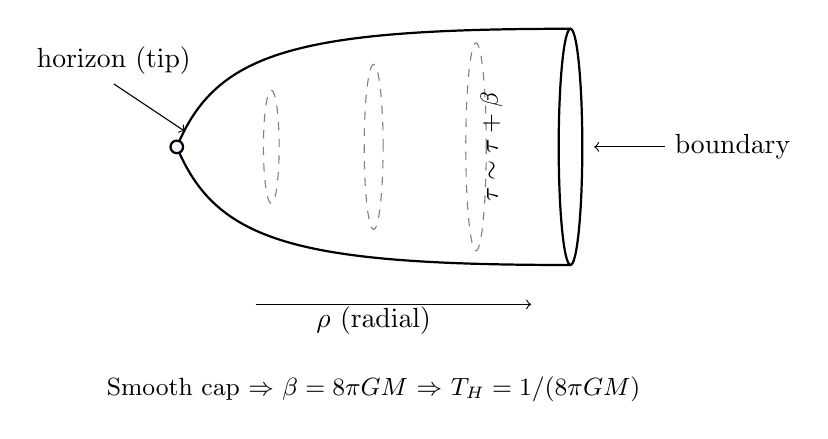
\begin{tikzpicture}[scale=1.0]
  \draw[thick] (0,0) .. controls (0.5,1.2) and (1.5,1.5) .. (5,1.5);
  \draw[thick] (0,0) .. controls (0.5,-1.2) and (1.5,-1.5) .. (5,-1.5);
  \draw[thick, fill=blue!5] (0,0) circle (0.08);
  \draw[thick] (5,0) ellipse (0.15 and 1.5);
  \draw[dashed, gray] (1.2,0) ellipse (0.1 and 0.72);
  \draw[dashed, gray] (2.5,0) ellipse (0.12 and 1.05);
  \draw[dashed, gray] (3.8,0) ellipse (0.13 and 1.32);
  \draw[<-] (0.1,0.2) -- (-0.8,0.8) node[above] {horizon (tip)};
  \draw[<-] (5.3,0) -- (6.2,0) node[right] {boundary};
  \node at (2.5, -2.2) {$\rho$ (radial)};
  \draw[->] (1.0, -2.0) -- (4.5, -2.0);
  \node[rotate=90] at (4.0, 0) {\small $\tau \sim \tau + \beta$};
  \node[below] at (2.5, -2.8)
    {\small Smooth cap $\Rightarrow$ $\beta = 8\pi GM$
    $\Rightarrow$ $T_H = 1/(8\pi GM)$};
\end{tikzpicture}
\end{adjustbox}
\caption{The Euclidean Schwarzschild black hole, often called the ``cigar''
geometry.  Euclidean time $\tau$ is periodic, forming circles (dashed) whose
radius shrinks to zero at the horizon, where the geometry smoothly caps off like
the tip of a cigar.  The requirement that this tip be smooth (no conical
singularity) fixes $\beta = 8\pi GM$, yielding the Hawking
temperature.}\label{fig05:cigar}
\end{figure}

The resulting geometry --- shown in Figure~\ref{fig05:cigar} --- is called the
\textbf{cigar} (or ``Euclidean cigar'').  It has the topology of a disk
$D^2 \times S^2$: the Euclidean time circle shrinks smoothly to zero size at the
horizon, so the $(\tau, r)$ part of the geometry looks like a disk, capping off
at its center.  There is no interior region; the Euclidean black hole has no
singularity or interior.  The entire geometry is the smooth region outside the
horizon, with the horizon itself realized as the smooth tip of the cigar.

\subsubsection*{The Euclidean action and black hole thermodynamics}

The Euclidean action of the Schwarzschild black hole, evaluated on the cigar
geometry with the Gibbons--Hawking--York boundary term properly included, gives
\citep{gibbonshawking1977}
\begin{equation}\label{eq05:euclidean_action_bh}
  I_{\mathrm{cigar}} \;=\; \beta\, F \;=\; \beta\, M - S_{\mathrm{BH}}\,,
\end{equation}
where $F$ is the free energy and
\begin{equation}\label{eq05:bh_entropy_from_action}
  S_{\mathrm{BH}} \;=\; \frac{A}{4G_N}
\end{equation}
is the Bekenstein--Hawking entropy \citep{bekenstein1973, hawking1975}.  Thus the
Euclidean path integral evaluated on the black hole saddle gives
$Z \approx e^{-I_{\mathrm{cigar}}} = e^{S_{\mathrm{BH}} - \beta M}$, which is
the formal saddle contribution $e^{-\beta F}$. Asymptotically flat
Schwarzschild has negative heat capacity and does not define a stable
canonical equilibrium in an infinite heat bath. A cavity, a suitable
finite reservoir, or a different stable branch is needed for an equilibrium
fluctuation calculation (Section~\ref{sec09:higher_dimensions}).  The entire edifice of black hole thermodynamics ---
temperature, entropy, free energy --- emerges naturally from the Euclidean
gravitational path integral.

\subsubsection*{The price of going Euclidean}

The Euclidean formulation is not without its difficulties.  Two issues are
particularly relevant for the developments in subsequent sections:

\begin{enumerate}
  \item \textbf{Euclidean saddles without Lorentzian continuations.}  Not every
    Euclidean saddle that contributes to the path integral has an obvious
    interpretation as a Lorentzian spacetime.  The replica wormholes that will
    appear in Section~\ref{sec06:replica_wormholes}
    \citep{pssyetal2022, ahmstetal2020} are a prime example: they are
    Euclidean geometries that connect $n$ copies of the spacetime, and for
    non-integer $n$ there is no literal $n$-fold cover. Continuation can
    instead be formulated using a quotient geometry with a conical defect.  Even for integer $n$, the Lorentzian interpretation of
    these geometries is subtle and has been the subject of considerable recent
    work \citep{colinetal2021}.

  \item \textbf{The conformal factor problem.}  The Euclidean Einstein--Hilbert
    action is not bounded below: conformal deformations
    $g_{\mu\nu} \to \Omega^2 g_{\mu\nu}$ can make the action arbitrarily
    negative.  The Euclidean path integral, taken literally, does not converge.
    In practice, this is handled by specifying a contour of integration for the
    conformal factor, but the procedure introduces ambiguities that are not fully
    resolved.
\end{enumerate}

Euclidean methods nevertheless provide well-tested semiclassical
calculations of Hawking temperature, black-hole entropy, and transitions
between admissible saddles. Their use requires the preparation, boundary
conditions, and approximation to remain explicit.

\bigskip
\noindent\textbf{Summary.} The gravitational path integral motivates a sum
over admissible geometries with quantum fluctuations around its saddles.
In JT gravity, fixed-boundary amplitudes admit a genus expansion with an
explicit topological weight. Matrix contractions provide a related planar
organization, but the weights and observables must be specified separately.
Euclidean regularity fixes the Schwarzschild temperature; it does not by
itself establish canonical stability. The next section applies replica
sewing to entropy and develops the normalized random-state benchmark.


\section{The Replica Trick and Replica Wormholes}
\label{sec06:replica_wormholes}

We develop the replica calculation first in a finite-dimensional random-state
model, where normalization and every combinatorial coefficient can be checked
exactly.  We then explain its relation to the microcanonical, flat-weight limit
of the west-coast model of replica wormholes.  The distinction matters: the
finite random-state formula is not a formula for every gravitational path
integral.  Within this benchmark, the complete planar sum resolves the
transition missed by retaining only the fully disconnected and fully connected
contractions.  The calculation also supplies the preparation for the
Marchenko--Pastur derivation in Section~\ref{sec07:free_probability}.

\subsection{The replica trick}
\label{subsec06:replica_trick}

Our goal is to compute the von Neumann entropy of the radiation:
\begin{equation}
\label{eq06:svn_target}
S_{\mathrm{vN}} = -\mathrm{Tr}(\rho \log \rho).
\end{equation}
The difficulty is the logarithm.  In a path integral formulation, $\rho$ is
computed as a functional integral over field configurations with specific
boundary conditions.  Taking the trace of $\rho$ raised to an integer power is
straightforward --- it amounts to gluing boundary conditions cyclically --- but
taking the logarithm of an operator defined by a path integral has no natural
geometric meaning.

The \emph{replica trick} circumvents this obstacle by exploiting a simple
identity.  For any positive operator $\rho$ with $\mathrm{Tr}\,\rho = 1$,
\begin{equation}
\label{eq06:replica_identity}
S_{\mathrm{vN}} = -\lim_{n \to 1} \frac{\partial}{\partial n}
  \mathrm{Tr}(\rho^n).
\end{equation}
The strategy is: (i)~compute $\mathrm{Tr}(\rho^n)$ for integer $n \geq 2$,
where the calculation has a clean geometric interpretation; (ii)~find a closed
form in $n$; (iii)~analytically continue to $n \to 1$ and differentiate.

\paragraph{Why this works.}
For integer $n \geq 2$, write $\rho$ in its eigenbasis:
$\rho = \sum_\alpha \lambda_\alpha |\alpha\rangle\langle\alpha|$, so that
$\mathrm{Tr}(\rho^n) = \sum_\alpha \lambda_\alpha^n$.  Each eigenvalue
satisfies $0 \leq \lambda_\alpha \leq 1$, so $\lambda_\alpha^n$ is a perfectly
well-defined analytic function of $n$ for all $\mathrm{Re}\,n > 0$.
Differentiating at $n = 1$:
\begin{equation}
\label{eq06:derivative_at_one}
-\frac{\partial}{\partial n} \lambda_\alpha^n \Big|_{n=1}
  = -\lambda_\alpha \log \lambda_\alpha,
\end{equation}
which, summed over $\alpha$, gives $S_{\mathrm{vN}}$.  For a fixed finite-dimensional state this continuation is supplied by its
spectrum, and $|\operatorname{Tr}\rho^z|\leq1$ for $\operatorname{Re}z\geq1$.
An arbitrary interpolation of integer replica data need not be unique:
a bound on the positive real axis alone does not control its growth in the
complex plane.  Section~\ref{subsec07:carlson} states the additional analytic
conditions used for the limiting Marchenko--Pastur moment integral.

\paragraph{The $n$-sheeted geometry.}
For integer $n$, the trace $\mathrm{Tr}(\rho^n)$ has a direct path-integral
interpretation.  Consider a quantum field theory on a Euclidean spacetime $M$,
and let $\rho$ be the reduced density matrix of a spatial region $A$, obtained
by tracing over the complement $\bar{A}$.  In the path-integral language,
$\rho$ is represented by cutting the Euclidean manifold along $A$ and leaving
the two sides of the cut as ``bra'' and ``ket'' boundary conditions.  To compute
$\mathrm{Tr}(\rho^n)$, one takes $n$ copies of this cut manifold and glues
them cyclically: the ket side of copy~$j$ is identified with the bra side of
copy~$j+1$ (with $n + 1 \equiv 1$).  The result is a partition function on an
$n$-sheeted branched cover $M_n$ of the original spacetime:
\begin{equation}
\label{eq06:n_sheeted_partition}
\mathrm{Tr}(\rho^n) = \frac{Z_n}{Z_1^n},
\end{equation}
where $Z_n = \int \mathcal{D}\phi\; e^{-I[\phi; M_n]}$ is the Euclidean
partition function on $M_n$ and $Z_1$ is the single-copy partition function
(the denominator ensures the correct normalization
$\mathrm{Tr}\,\rho = 1$).

Figure~\ref{fig06:n_sheeted} illustrates this construction for $n = 3$.  Three
copies of the spacetime are arranged in a stack, each cut along the region $A$.
The cyclic gluing $1 \to 2 \to 3 \to 1$ produces a three-sheeted cover with a
branch point at the boundary $\partial A$.

\begin{figure}[htbp]
\centering
\begin{adjustbox}{max width=\textwidth, center}
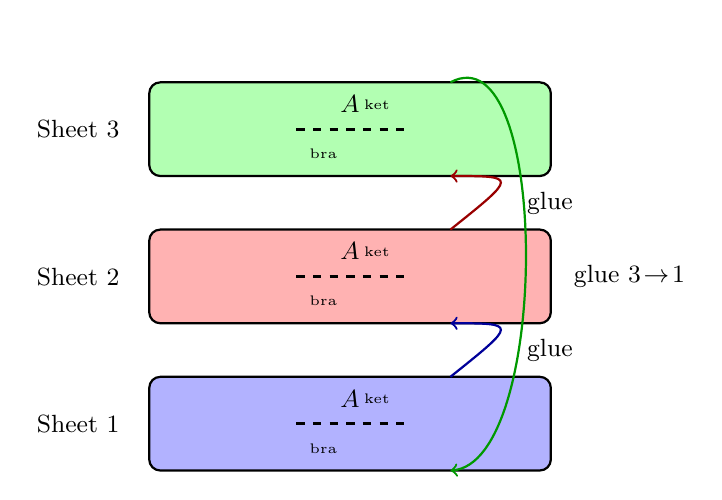
\begin{tikzpicture}[scale=0.85]
  \foreach \s/\yshift/\col in {1/0/blue!30, 2/2.2/red!30, 3/4.4/green!30} {
    \begin{scope}[yshift=\yshift cm]
      \fill[\col, rounded corners=4pt] (-3,-0.7) rectangle (3,0.7);
      \draw[thick, rounded corners=4pt] (-3,-0.7) rectangle (3,0.7);
      \draw[very thick, dashed] (-0.8,0) -- (0.8,0);
      \node[above] at (0,0.1) {\small $A$};
      \node[left] at (-3.3,0) {\small Sheet \s};
      \node[below, font=\tiny] at (-0.4,-0.15) {bra};
      \node[above, font=\tiny] at (0.4,0.15) {ket};
    \end{scope}
  }
  \draw[->, thick, blue!60!black] (1.5,0.7) .. controls (2.5,1.5) .. (1.5,1.5);
  \node[right, font=\small] at (2.5,1.1) {glue};
  \draw[->, thick, red!60!black] (1.5,2.9) .. controls (2.5,3.7) .. (1.5,3.7);
  \node[right, font=\small] at (2.5,3.3) {glue};
  \draw[->, thick, green!60!black] (1.5,5.1) .. controls (3.0,5.9)
    and (3.0,-0.6) .. (1.5,-0.7);
  \node[right, font=\small] at (3.2,2.2) {glue $3 \!\to\! 1$};
\end{tikzpicture}
\end{adjustbox}
\caption{The $n$-sheeted replica geometry for $n = 3$.  Each sheet represents
one copy of the Euclidean spacetime, cut along the entangling region $A$.  The
cyclic identification (ket of sheet $j$ $\to$ bra of sheet $j+1$, with
$3+1 \equiv 1$) produces the branched cover $M_3$.}
\label{fig06:n_sheeted}
\end{figure}

\paragraph{In gravity: dynamical topology.}
In a non-gravitational QFT, the manifold $M_n$ is fixed and the path integral
sums only over fields on that manifold.  In a theory of gravity, the manifold
itself is dynamical. A chosen gravitational path integral may include
connected bulk geometries with the prescribed replicated boundary data.
A stationary geometry connecting distinct replicas is called a
\emph{replica wormhole}. Whether a topology admits a contributing saddle,
and with what weight, depends on the theory, boundary conditions, and
integration contour. The flat-weight model below makes the relevant
replica contractions explicit.

The rest of this section makes this idea precise in the simplest possible
context: the west-coast model.

\subsection{The west-coast model}
\label{subsec06:pssy_model}

The west-coast model, introduced by Penington, Shenker, Stanford, and
Yang~\citep{pssyetal2022} (building on the JT gravity framework
of~\citet{saadetal2019}), is a solvable toy model that captures the essential
physics of replica wormholes while remaining exactly computable.  It consists
of Jackiw--Teitelboim (JT) gravity on a disk with $k$ flavors of
end-of-the-world (EOW) branes.

\paragraph{The Hilbert space and the flat-weight approximation.}
For the finite-dimensional benchmark let
$\mathcal H_{\mathrm{BH}}=\mathbb C^L$ and
$\mathcal H_{\mathrm{rad}}=\mathbb C^k$.  The gravitational interpretation
requires a chosen microcanonical energy window and approximately constant
state-preparation weights in that window.  Its effective number of black-hole
states is represented by $L$; writing $L=e^{S_0}$ is a useful simplified
counting convention, not an identity between the full JT Hilbert space and a
finite space of that dimension.  In a canonical JT preparation the energy
density and brane weights must instead be retained.

We write $\gamma=k/L$.  Scanning $k$ at fixed $L$ gives a family of states
with an entanglement crossover at $\gamma=1$.  It does not specify a unitary
evaporation channel.  A dynamical model may have dimensions $k(t)$ and $L(t)$;
its time dependence and energy constraints require separate assumptions.

\paragraph{The state.}
The combined state of the black hole and radiation is
\begin{equation}
\label{eq06:psi_state}
|\psi\rangle = \frac{1}{\sqrt{Z}} \sum_{i=1}^{k}
  |\psi_i\rangle_{\mathrm{BH}} \otimes |i\rangle_{\mathrm{rad}},
\end{equation}
where $|\psi_i\rangle_{\mathrm{BH}}$ is the state of the black hole interior
conditioned on having emitted a brane of flavor~$i$, and
$Z = \sum_{i} \langle \psi_i | \psi_i \rangle$ is the normalization.  This
state is the gravity analog of a random bipartite pure state: if the states
$|\psi_i\rangle$ were orthonormal, $|\psi\rangle$ would simply be a maximally
entangled state of Schmidt rank $k$.  The key point is that the overlaps
$\langle \psi_j | \psi_i \rangle$ are \emph{not} specified a priori --- they are
computed by the gravitational path integral.

\paragraph{Overlaps from gravity.}
The overlap $\langle \psi_j | \psi_i \rangle$ is computed by a Euclidean path
integral on a manifold whose boundary conditions require brane flavor~$i$ on one
side and flavor~$j$ on the other.  At leading order (disk topology), only the
$i = j$ boundary condition admits a solution:
\begin{equation}
\label{eq06:overlap_disk}
\mathbb E\langle \psi_j | \psi_i \rangle\big|_{\text{flat disk}} = L \, \delta_{ij}.
\end{equation}
Replacing the overlaps and the normalization by these disk means gives
\begin{equation}
\label{eq06:rho_rad_leading}
 \rho_{\mathrm{disc}}
 =\frac{1}{kL}\sum_{i,j}\mathbb E\langle\psi_j|\psi_i\rangle
 |i\rangle\langle j|=\frac{\mathbb 1_k}{k}.
\end{equation}
This is the disconnected approximation. In the isotropic Gaussian benchmark,
unitary invariance also gives $\mathbb E\rho_{\mathrm{rad}}=\mathbb 1_k/k$
for the exactly normalized states. Neither statement identifies individual
realizations with their average. In particular, for $k>L$ every realization
has rank at most $L$, whereas its averaged matrix has rank $k$.
Products of overlaps have connected contributions even when their individual
means vanish.  These contributions restore the nontrivial spectral moments;
computing a moment of the averaged matrix would discard them.

\paragraph{The density matrix and its moments.}
Tracing over the black hole yields
\begin{equation*}
\rho_{\mathrm{rad}} = Z^{-1} \sum_{i,j}
\langle\psi_j|\psi_i\rangle\,|i\rangle\langle j|.
\end{equation*}
The $n$th moment of $\rho_{\mathrm{rad}}$ involves a product of $n$ such
overlaps, summed over brane indices in the pattern dictated by the cyclic trace:
\begin{equation}
\label{eq06:trace_rho_n}
\mathrm{Tr}(\rho_{\mathrm{rad}}^n)
  = \frac{1}{Z^n} \sum_{i_1, \ldots, i_n}
    \langle \psi_{i_2}|\psi_{i_1}\rangle
    \langle \psi_{i_3}|\psi_{i_2}\rangle
    \cdots
    \langle \psi_{i_1}|\psi_{i_n}\rangle.
\end{equation}
Each product of overlaps is now computed by a gravitational path integral on
$n$ copies of the disk, with the crucial point being that the bulk geometry is
free to connect these copies through wormholes.  The different topological
connections are labeled by permutations, as we explain next.

\subsection{The master formula: permutations and topology}
\label{subsec06:master_formula}

Let $G$ be a $k\times L$ matrix of independent standard complex Gaussian
entries and set
\begin{equation}
 W=GG^\dagger,\qquad T=\operatorname{Tr}W,\qquad
 \rho=\frac WT,\qquad \widetilde\rho=\frac W{kL}.
 \label{eq06:normalizations}
\end{equation}
The matrix $\rho$ is the reduction of a normalized Haar-random pure state.
The matrix $\widetilde\rho$ has unit trace only in expectation.  Write
$c_n=(1\,2\cdots n)$, let $C(\sigma)$ count cycles, and define
$(D)_n=D(D+1)\cdots(D+n-1)$.  The exact normalized formula is
\begin{equation}
 \boxed{\quad
 \mathbb E_{\mathrm H}\operatorname{Tr}\rho^n
 =\frac{1}{(kL)_n}\sum_{\sigma\in S_n}
 k^{C(c_n^{-1}\sigma)}L^{C(\sigma)}.\quad}
 \label{eq06:pssy_master}
\end{equation}
Here the expectation is over Haar states.  The cycle orientation can be
reversed by relabelling the permutations; it must be kept consistent with the
chosen trace convention.

\paragraph{Derivation and the role of normalization.}
Expanding $\operatorname{Tr}W^n$ produces $n$ Gaussian entries and $n$
conjugate entries.  Wick's rule pairs them according to $\sigma\in S_n$.
The black-hole indices form $C(\sigma)$ independent loops, each contributing
$L$.  The cyclic radiation trace leaves $C(c_n^{-1}\sigma)$ loops, each
contributing $k$.  Thus the numerator in Eq.~\eqref{eq06:pssy_master} is
$\mathbb E\operatorname{Tr}W^n$.

The Gaussian vector of $kL$ entries has independent radial and angular parts.
Its squared norm $T$ has the gamma distribution with shape $kL$ and unit scale,
so $\mathbb E T^n=(kL)_n$.  The angular part is a Haar vector, and
$W=T\rho$ with $T$ independent of $\rho$.  Dividing
$\mathbb E\operatorname{Tr}W^n=\mathbb E T^n\,
\mathbb E_{\mathrm H}\operatorname{Tr}\rho^n$ proves the formula.
For the alternative normalization one obtains instead
\begin{equation}
 \mathbb E\operatorname{Tr}\widetilde\rho^n
 =(kL)^{-n}\sum_{\sigma\in S_n}
 k^{C(c_n^{-1}\sigma)}L^{C(\sigma)},\qquad
 \mathbb E_{\mathrm H}\operatorname{Tr}\rho^n
 =\frac{(kL)^n}{(kL)_n}\,
 \mathbb E\operatorname{Tr}\widetilde\rho^n.
 \label{eq06:mean_normalized_master}
\end{equation}
This second formula is convenient for organizing Wick contractions by genus.
For fixed $n$ and fixed positive $k/L$, the prefactor approaches one with
relative corrections of order $(kL)^{-1}$, but these corrections cannot be
omitted in a finite-size calculation.

\paragraph{A two-qubit normalization check.}
At $n=2$, the identity and transposition give
\begin{equation}
 \mathbb E_{\mathrm H}\operatorname{Tr}\rho^2
 =\frac{k+L}{kL+1},\qquad
 \mathbb E\operatorname{Tr}\widetilde\rho^2=\frac1k+\frac1L.
 \label{eq06:exact_purity}
\end{equation}
The normalized result is Lubkin's mean-purity formula~\citep{lubkin1978}.
For two qubits, $k=L=2$, it is $4/5$, whereas the mean-normalized expression
is $1$.  For $k=1$ the normalized reduced state is necessarily pure and the
first formula gives $1$ exactly; the second gives $1+1/L$.  These elementary
checks identify the object being computed before any replica continuation.
The Gaussian normalization of $\widetilde\rho$ is not a harmless exact
replacement for normalization of each state.

\paragraph{What carries over to gravity.}
In the microcanonical flat-weight approximation, the cycle factors reproduce
the corresponding replica contractions of the west-coast model
\citep{pssyetal2022}.  The factors $L^{C(\sigma)}$ are index-loop factors
in the Gaussian derivation, not propagating graviton loops.  General JT
preparations assign energy-dependent partition functions to connected
components.  Their planar sums retain non-crossing combinatorics but need
not give the same Marchenko--Pastur law.  Additional continuum handles and
moduli integrals are not enumerated by this finite Wick sum.

\paragraph{The genus of a permutation.}
Not all permutations contribute at the same order.  The ribbon graph associated with a Wick contraction has a genus:
\begin{equation}
\label{eq06:genus_formula}
g(\sigma) = \frac{n + 1 - C(\sigma) - C(c_n^{-1}\sigma)}{2}.
\end{equation}
This formula has a precise topological origin: the permutation $\sigma$
and the fixed cyclic permutation $c_n$ together define a branched covering
of the sphere, and $g(\sigma)$ is the genus of the covering surface (by the
Riemann--Hurwitz formula).  At fixed $n$ and fixed $\gamma\in(0,\infty)$, each additional genus
costs two powers of a dimension.  If $L=e^{S_0}$ is adopted as the counting
convention, this is the factor $e^{-2gS_0}$, up to fixed ratio factors.
This is a statement about the Gaussian index expansion.

Rewriting Eq.~\eqref{eq06:mean_normalized_master} makes this expansion explicit:
\begin{equation}
\label{eq06:genus_expansion}
\mathbb E\operatorname{Tr}(\widetilde\rho^n) = k^{1-n}
  \sum_{\sigma \in S_n} k^{-2g(\sigma)} \, \gamma^{n - C(\sigma)},
\end{equation}
where $\gamma = k/L$ and we have used
$C(c_n^{-1}\sigma) = n + 1 - C(\sigma) - 2g(\sigma)$ to write the
per-permutation weight as
$(kL)^{-n}\, k^{C(c_n^{-1}\sigma)} L^{C(\sigma)}
= k^{1-n-2g(\sigma)}\,\gamma^{n - C(\sigma)}$, eliminating
$C(c_n^{-1}\sigma)$ in favor of $g(\sigma)$ and $C(\sigma)$.

\paragraph{The genus-zero sector: non-crossing permutations.}
The genus-zero condition $g(\sigma) = 0$ is equivalent to
\begin{equation}
\label{eq06:genus_zero_condition}
C(\sigma) + C(c_n^{-1}\sigma) = n + 1.
\end{equation}
Permutations satisfying this condition are precisely the \emph{non-crossing
permutations} $\mathrm{NC}(n)$: each block is written as a cycle in the
cyclic order inherited from $c_n$.  This orientation is part of the definition.
These are the permutations that, when
represented as connection patterns on $n$ points arranged on a circle
(in the order dictated by $c_n$), have no crossings.  The number of
non-crossing permutations of $n$ elements is the \emph{Catalan
number}:
\begin{equation}
\label{eq06:catalan_number}
|\mathrm{NC}(n)| = C_n = \frac{1}{n+1}\binom{2n}{n}.
\end{equation}
The first few values are $C_1 = 1$, $C_2 = 2$, $C_3 = 5$, $C_4 = 14$,
$C_5 = 42$, $C_6 = 132$, $C_7 = 429$.

\paragraph{Graphical interpretation.}
The connection between permutations and non-crossing partitions has a vivid
graphical representation, shown in Figure~\ref{fig06:non_crossing}.  Place
the numbers $1, 2, \ldots, n$ on a circle in the order determined by the
cyclic permutation $c_n$.  For each cycle $(a_1\; a_2\; \cdots\; a_m)$ of
$\sigma$, draw arcs connecting $a_1 \to a_2 \to \cdots \to a_m \to a_1$.  If the cycles follow the prescribed orientation and
their polygons have disjoint interiors, the permutation
is non-crossing and contributes at genus zero.  If crossings are unavoidable,
the permutation has $g(\sigma) \geq 1$ and is suppressed by at least
$L^{-2} = e^{-2S_0}$.

\begin{figure}[htbp]
\centering
\begin{adjustbox}{max width=\textwidth, center}
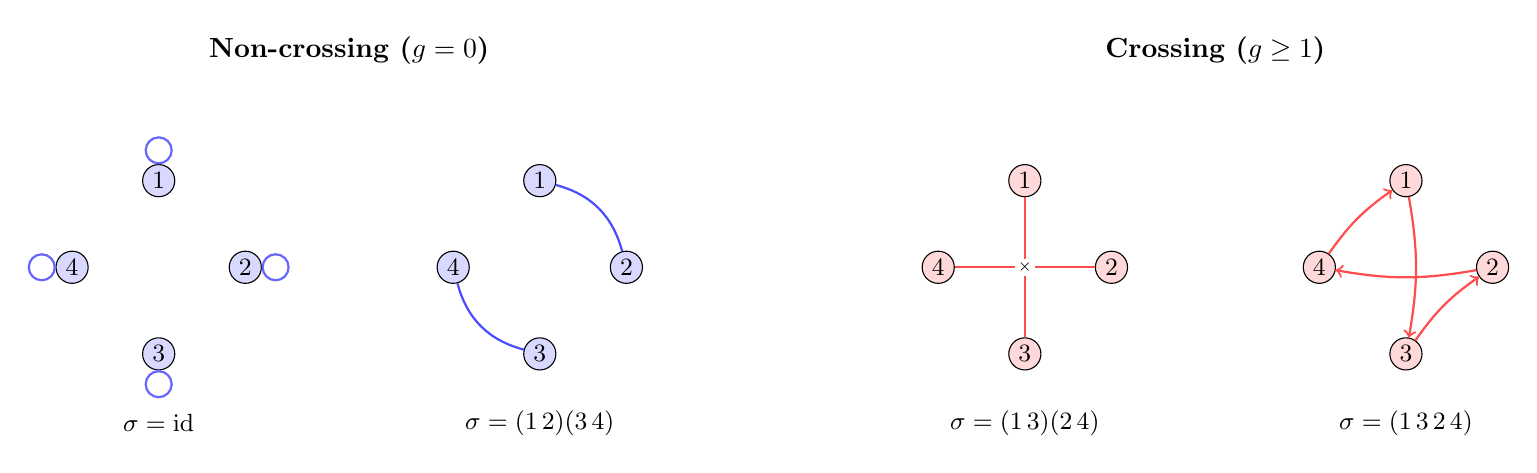
\begin{tikzpicture}[scale=1.1]
  \begin{scope}[xshift=-5cm]
    \node[font=\bfseries] at (0,2.0) {Non-crossing ($g = 0$)};

    \begin{scope}[xshift=-2.2cm, yshift=-0.5cm]
      \node[font=\small] at (0,-1.8) {$\sigma = \mathrm{id}$};
      \foreach \i/\angle in {1/90, 2/0, 3/270, 4/180} {
        \node[circle, draw, fill=blue!15, inner sep=1.5pt,
              font=\small] (\i) at (\angle:1.0) {\i};
      }
      \foreach \i/\angle in {1/90, 2/0, 3/270, 4/180} {
        \draw[thick, blue!60] (\angle:1.35) circle (0.15);
      }
    \end{scope}

    \begin{scope}[xshift=2.2cm, yshift=-0.5cm]
      \node[font=\small] at (0,-1.8) {$\sigma = (1\,2)(3\,4)$};
      \foreach \i/\angle in {1/90, 2/0, 3/270, 4/180} {
        \node[circle, draw, fill=blue!15, inner sep=1.5pt,
              font=\small] (\i) at (\angle:1.0) {\i};
      }
      \draw[thick, blue!70, bend left=30] (1) to (2);
      \draw[thick, blue!70, bend left=30] (3) to (4);
    \end{scope}
  \end{scope}

  \begin{scope}[xshift=5cm]
    \node[font=\bfseries] at (0,2.0) {Crossing ($g \geq 1$)};

    \begin{scope}[xshift=-2.2cm, yshift=-0.5cm]
      \node[font=\small] at (0,-1.8) {$\sigma = (1\,3)(2\,4)$};
      \foreach \i/\angle in {1/90, 2/0, 3/270, 4/180} {
        \node[circle, draw, fill=red!15, inner sep=1.5pt,
              font=\small] (\i) at (\angle:1.0) {\i};
      }
      \draw[thick, red!70] (1) -- (3);
      \draw[thick, red!70] (2) -- (4);
      \node[font=\tiny, fill=white, inner sep=1pt] at (0,0) {$\times$};
    \end{scope}

    \begin{scope}[xshift=2.2cm, yshift=-0.5cm]
      \node[font=\small] at (0,-1.8) {$\sigma = (1\,3\,2\,4)$};
      \foreach \i/\angle in {1/90, 2/0, 3/270, 4/180} {
        \node[circle, draw, fill=red!15, inner sep=1.5pt,
              font=\small] (\i) at (\angle:1.0) {\i};
      }
      \draw[thick, red!70, ->, bend left=10] (1) to (3);
      \draw[thick, red!70, ->, bend left=10] (3) to (2);
      \draw[thick, red!70, ->, bend left=10] (2) to (4);
      \draw[thick, red!70, ->, bend left=10] (4) to (1);
    \end{scope}
  \end{scope}
\end{tikzpicture}
\end{adjustbox}
\caption{Permutations of $n=4$ elements arranged on a circle in the order
$(1,2,3,4)$ determined by the cyclic permutation $c_n$.  \textbf{Left:}
Non-crossing permutations (genus~$0$): the identity $\sigma = \mathrm{id}$ has
four fixed points (self-loops), and $\sigma = (1\,2)(3\,4)$ has two
non-crossing transpositions of adjacent elements.  \textbf{Right:} Crossing
permutations (genus~$\geq 1$): $\sigma = (1\,3)(2\,4)$ forces the arcs
$1$--$3$ and $2$--$4$ to cross, and the $4$-cycle $\sigma = (1\,3\,2\,4)$
similarly produces unavoidable crossings.  At genus zero, only non-crossing
permutations contribute, and for $n = 4$ there are $C_4 = 14$ of them versus
$4! = 24$ total.}
\label{fig06:non_crossing}
\end{figure}

\paragraph{The genus-zero moment.}
Restricting Eq.~\eqref{eq06:mean_normalized_master} to genus zero, and
using the genus-zero constraint $C(c_n^{-1}\sigma) = n + 1 - C(\sigma)$ to
simplify:
\begin{equation}
\label{eq06:genus_zero_moment}
\boxed{
\mathbb E\operatorname{Tr}(\widetilde\rho^n)\big|_{g=0}
  = k^{1-n} \sum_{\sigma \in \mathrm{NC}(n)} \gamma^{n - C(\sigma)}
  = k^{1-n} \, M_n(\gamma)
}
\end{equation}
where $M_n(\gamma) = \sum_{\sigma \in \mathrm{NC}(n)} \gamma^{n - C(\sigma)}$
is the $n$th moment of the Marchenko--Pastur distribution with
parameter~$\gamma$ \citep{marchenkopastur1967}.  (As a check, at $n = 2$ this
gives $\mathrm{Tr}(\rho^2)|_{g=0} = k^{-1}(1 + \gamma) = 1/k + 1/L$, the leading large-dimension purity.)  The combination of the non-crossing combinatorics and these flat cycle weights
determines the distribution.  For normalized Haar states the precise limiting
statement is $k^{n-1}\mathbb E_{\mathrm H}\operatorname{Tr}\rho^n
\to M_n(\gamma)$ for fixed $n$, as developed in
Section~\ref{sec07:free_probability}.

The non-crossing permutations can be further organized by cycle number using
the \emph{Narayana numbers} $N(n,j) = \frac{1}{n}\binom{n}{j}\binom{n}{j-1}$,
which count the number of non-crossing permutations with exactly $j$ cycles:
\begin{equation}
\label{eq06:narayana_decomposition}
M_n(\gamma) = \sum_{j=1}^{n} N(n,j)\,\gamma^{n-j}.
\end{equation}
Each Narayana stratum $N(n,j)$ represents a family of partially connected
topologies with the same number of bulk connected components, and the Narayana
decomposition organizes the genus-zero sector into a hierarchy of increasing
connectivity.

\subsection{The two-saddle approximation and its failure}
\label{subsec06:two_saddle}

The leading saddle comparison underlying the island transition
\citep{penington2020,almheirietal2019,almheirietal2020islands} motivates keeping
two extreme contractions.  In the flat-weight model these are the following
terms of Eq.~\eqref{eq06:mean_normalized_master}.  The complete planar sum
was already included in the resolvent analysis of~\citet{pssyetal2022}.
\begin{enumerate}
\item \textbf{The identity} $\sigma = \mathrm{id}$, corresponding to fully
  \emph{disconnected} replicas.  This permutation has $C(\mathrm{id}) = n$
  cycles (every element is a fixed point) and $C(c_n^{-1}\mathrm{id}) =
  C(c_n^{-1}) = 1$ cycle.  Its contribution is
  \begin{equation}
  \label{eq06:id_contribution}
  \mathbb E\operatorname{Tr}(\widetilde\rho^n)\big|_{\mathrm{id}} = (kL)^{-n} \cdot k^1 \cdot L^n
    = k^{1-n}.
  \end{equation}
  In units of the overall genus-zero prefactor $k^{1-n}$, this is the $\gamma^0$ term in the Narayana expansion (the $j = n$ stratum, with $N(n,n) = 1$).

\item \textbf{The cyclic permutation} $\sigma = c_n = (1\;2\;\cdots\;n)$,
  corresponding to the fully \emph{connected} wormhole.  This permutation has
  $C(c_n) = 1$ cycle and
  $C(c_n^{-1}c_n) = C(\mathrm{id}) = n$ cycles.  Its contribution is
  \begin{equation}
  \label{eq06:gamma_contribution}
  \mathbb E\operatorname{Tr}(\widetilde\rho^n)\big|_{c_n} = (kL)^{-n} \cdot k^n \cdot L^1
    = L^{1-n} = k^{1-n}\,\gamma^{n-1}.
  \end{equation}
  This is the $j = 1$ stratum (Narayana number $N(n,1) = 1$), with the highest
  power of $\gamma$.
\end{enumerate}

These are the two extreme Narayana strata --- $j = n$ (the identity) and $j = 1$ (the full cycle) --- each of which contains a single permutation, since $N(n,n) = N(n,1) = 1$.  Together they give the \emph{two-saddle approximation}:
\begin{equation}
\label{eq06:two_saddle_formula}
\mathbb E\operatorname{Tr}(\widetilde\rho^n)_{\text{two-saddle}}
  = k^{1-n}\bigl(1 + \gamma^{n-1}\bigr) = k^{1-n} + L^{1-n}.
\end{equation}

\paragraph{What is missing.}
For $n \geq 3$, there are $C_n - 2$ additional non-crossing permutations that
are neither the identity nor the full cycle.  These correspond to
\emph{partially connected} wormhole topologies: configurations where some ---
but not all --- of the $n$ replicas are connected through the bulk.  In the flat-weight replica model these are additional planar contractions.
At fixed $\gamma$, each contributes at the same order in the dimension
expansion as the identity and cyclic contractions.

The exact genus-zero result is
\begin{equation}
\label{eq06:exact_genus_zero}
\mathbb E\operatorname{Tr}(\widetilde\rho^n)\big|_{g=0}
  = k^{1-n} \sum_{j=1}^{n} N(n,j)\,\gamma^{n-j}
  = k^{1-n}\,M_n(\gamma),
\end{equation}
while the two-saddle approximation retains only the $j = 1$ and $j = n$ terms.
The error is
\begin{equation}
\label{eq06:missing_saddles}
\mathbb E\operatorname{Tr}(\widetilde\rho^n)\big|_{g=0} - \mathbb E\operatorname{Tr}(\widetilde\rho^n)_{\text{two-saddle}}
  = k^{1-n} \sum_{j=2}^{n-1} N(n,j)\,\gamma^{n-j},
\end{equation}
which involves $\sum_{j=2}^{n-1} N(n,j) = C_n - 2$ permutations.

\paragraph{The error at the Page time.}
The failure is most dramatic at the Page time $\gamma = 1$ ($k = L$), where
every non-crossing permutation contributes equally:
\begin{equation}
\label{eq06:page_time_error}
\frac{\mathbb E\operatorname{Tr}(\widetilde\rho^n)\big|_{g=0}}
     {\mathbb E\operatorname{Tr}(\widetilde\rho^n)_{\text{two-saddle}}} \bigg|_{\gamma = 1}
= \frac{\sum_{j=1}^{n} N(n,j)}{1 + 1}
= \frac{C_n}{2}.
\end{equation}
This ratio grows rapidly with $n$.  Using the asymptotic form of the Catalan
numbers, $C_n \sim 4^n / (n^{3/2}\sqrt{\pi})$, the error grows as
\begin{equation}
\label{eq06:error_asymptotics}
\frac{C_n}{2} \sim \frac{4^n}{2\,n^{3/2}\sqrt{\pi}},
\end{equation}
which is \emph{exponential} in $n$.  This is a ratio of planar integer moments for $n\geq2$.  By itself it does
not determine the error in a derivative at $n=1$.  That entropy error must be
computed from the full limiting density, which is done in the next section.
The large-$n$ asymptotic displayed here is not a claim that the fixed-$n$
planar expansion is uniform at arbitrarily large replica index.

Table~\ref{tab06:two_saddle_error} displays the ratio $C_n/2$ for small
values of $n$, along with the number of missing saddles $C_n - 2$.

\begin{table}[htbp]
\centering
\caption{Failure of the two-saddle approximation at the Page time
$\gamma = 1$.  The ratio
$\mathbb E\operatorname{Tr}(\widetilde\rho^n)|_{g=0}\,/\,\mathbb E\operatorname{Tr}(\widetilde\rho^n)_{\text{two-saddle}}
= C_n/2$ measures the multiplicative error from omitting partially connected
wormholes.  The number of missing genus-zero saddles is $C_n - 2$.}
\label{tab06:two_saddle_error}
\begin{adjustbox}{max width=\textwidth,center}
\begin{tabular}{c c c c c}
\hline\hline
$n$ & $C_n$ & $C_n - 2$ (missing saddles) &
  $C_n/2$ (error ratio) & $4^n/(2n^{3/2}\sqrt{\pi})$ \\
\hline
2 & 2  & 0   & 1.00  & 1.60 \\
3 & 5  & 3   & 2.50  & 3.47 \\
4 & 14 & 12  & 7.00  & 9.03 \\
5 & 42 & 40  & 21.00 & 25.84 \\
6 & 132 & 130 & 66.00 & 78.62 \\
7 & 429 & 427 & 214.50 & 249.56 \\
\hline\hline
\end{tabular}
\end{adjustbox}
\end{table}

Several features of Table~\ref{tab06:two_saddle_error} deserve comment:
\begin{itemize}
\item For $n = 2$, the two-term sum exhausts the Wick numerator: there are only
  $C_2 = 2$ non-crossing permutations (the identity and the transposition), and
  both are included.  The exact normalized moment still requires the denominator $kL(kL+1)$.
  In addition, the logarithm of a mean purity and the mean logarithm of purity
  are different ensemble quantities.

\item For $n = 3$, three partially connected saddles are already missing, and the
  error ratio is $5/2 = 2.5$.  The two-saddle answer underestimates
  the planar mean-normalized third moment by a factor of $2.5$ at $k=L$.

\item For $n = 7$, the two-saddle approximation misses $427$ of the $429$
  genus-zero topologies, and the error exceeds a factor of $200$.

\item The exact ratio $C_n/2$ approaches the asymptotic form
  $4^n/(2n^{3/2}\sqrt{\pi})$ from below.  The convergence is somewhat slow
  (the ratio of exact to asymptotic is still $\approx 0.86$ at $n = 7$)
  because the sub-leading corrections to the Catalan asymptotics are
  significant for small $n$.
\end{itemize}

\paragraph{Physical interpretation.}
The partially connected wormholes that the two-saddle approximation
discards have a clear physical meaning.  They are topologies in which
\emph{some} replicas are connected by wormholes while others remain
disconnected.  For example, at $n = 4$, the permutation
$\sigma = (1\,2)(3)(4)$ describes a configuration where replicas $1$ and $2$
are connected through a wormhole while replicas $3$ and $4$ remain
independent.  This permutation has $C(\sigma) = 3$ cycles and contributes
at genus zero (one can verify that the arcs do not cross on the circle
diagram).

The reason these partially connected topologies matter is that, near the
Page transition, the fully disconnected and fully connected saddles are
comparable in magnitude (both scale as $L^{1-n}$ when $\gamma = 1$), and
the partially connected saddles are \emph{also} comparable.  There is no
parametric suppression of one saddle relative to another at $\gamma = 1$;
all $C_n$ genus-zero saddles contribute on an equal footing.  Selecting just the dominant saddle replaces the crossover by a switch
between the two extreme contractions.  The complete planar spectral law
resolves the associated entropy cusp.  Keeping their sum at integer $n$
and selecting a dominant entropy saddle are distinct approximations.

\paragraph{Consequences for the von Neumann entropy.}
For $n\geq2$ the two extreme contractions give a useful asymptotic description
when one dimension is much larger than the other.  Adding those two terms and
then setting $n=1$ would count the same identity contraction twice: the result
would be $2$ rather than $1$.  Thus the two-term integer formula is not itself
a normalized replica continuation near one.

The full planar sum avoids this ambiguity by specifying a probability density.
Its entropy deficit at $k=L$ is $1/2$ nat in the large-dimension limit.  That
constant is the leading Page correction~\citep{page1993}, and its replica
resolvent derivation appears in~\citet{pssyetal2022}; see also the discussion of
partially connected saddles in~\citet{marolfmaxfield2020}.  The Narayana
organization in the companion paper~\citep{wuebben2026paper1} makes the
contributions of each cycle count explicit.  It does not introduce a new
planar entropy law.

\subsection{Summary: from permutations to distributions}
\label{subsec06:summary}

The replica trace fixes a cyclic ordering; Wick contractions provide a
permutation sum; and the leading contractions at fixed dimension ratio are
non-crossing.  For normalized Haar states, the rising factorial in
Eq.~\eqref{eq06:pssy_master} is part of the exact answer.  The mean-normalized
formula is useful bookkeeping for the planar limit, where its Narayana
polynomial becomes the Marchenko--Pastur moment.  This chain of statements
explains why the flat-weight gravitational model has random-state spectral
statistics, while leaving energy weights and continuum topology to their
separate gravitational calculation.


\part{Free Probability and the Marchenko--Pastur Distribution}

\section{Free Probability and the Planar Random-State Limit}
\label{sec07:free_probability}

Section~\ref{sec06:replica_wormholes} reduced the flat-weight replica
calculation to a sum over non-crossing partitions.  We now derive its limiting
spectral density, the Marchenko--Pastur law, and then its entropy.  The
calculation is a concrete application of free probability, with all cycle
weights specified.  Non-crossing combinatorics alone would not determine this
particular law.

The gravitational use of free probability has a broader established form.
\citet{wang2023} identifies a free multiplicative convolution in the
west-coast model, with gravitational partition functions entering the free
cumulants.  \citet{chengetal2024} obtain related laws for random tensor
networks and competing cuts.  The simple Marchenko--Pastur law discussed here
requires the flat cycle weights of the finite-dimensional benchmark; more
general matter spectra and energy-dependent gravitational weights give other
free convolutions.  We use the moment--cumulant formalism of
Speicher~\cite{speicher1994} within Voiculescu's free
probability~\cite{voiculescu1991}.

The result connects three familiar calculations: the planar Wick sum, the
large-dimension spectrum of a reduced Haar state, and the leading Page
entropy~\cite{marchenkopastur1967,lubkin1978,lloydpagels1988,page1993}.
The companion paper~\cite{wuebben2026paper1} develops the cycle-count
organization and the effect of non-flat preparation weights.  This section
supplies the background needed to understand those distinctions.

\subsection{Classical vs.\ free probability}
\label{subsec07:classical_vs_free}

We begin with a brief comparison of classical and free probability,
emphasizing the single structural change --- the restriction from all
partitions to non-crossing partitions --- that connects the two theories.

\paragraph{Classical independence.}
In classical probability, independence of $X$ and $Y$ implies factorization
of their joint moments whenever those moments exist:
\begin{equation}
  \mathbb{E}[X^m Y^n] = \mathbb{E}[X^m]\,\mathbb{E}[Y^n].
  \label{eq07:classical_independence}
\end{equation}
The moment-cumulant relation expresses moments in terms of cumulants
$\chi_m$ by summing over \emph{all} partitions of the set $\{1,2,\ldots,n\}$:
\begin{equation}
  M_n \;=\; \sum_{\pi \in \mathcal{P}(n)} \;\prod_{B \in \pi} \chi_{|B|},
  \label{eq07:classical_moment_cumulant}
\end{equation}
where $\mathcal{P}(n)$ denotes the set of all set partitions of
$\{1,\ldots,n\}$ and the product runs over the blocks $B$ of the
partition $\pi$.  The number of partitions $|\mathcal{P}(n)|$ is the
Bell number $B_n$; the first few values are $B_1=1$, $B_2=2$, $B_3=5$,
$B_4=15$, $B_5=52$.

\paragraph{Free independence.}
Free probability, introduced by Voiculescu \cite{voiculescu1991}, replaces
the notion of independence with \emph{free independence} (or
\emph{freeness}), a non-commutative analogue appropriate for operators on
a Hilbert space.  More precisely, unital subalgebras are free with respect to a normalized
trace $\tau$ when $\tau(a_1\cdots a_r)=0$ for centered elements
$\tau(a_j)=0$ from alternating subalgebras.  This condition replaces the
factorization used for independent commuting variables.  Its combinatorial
consequence is
the moment-cumulant relation~\eqref{eq07:classical_moment_cumulant} is
replaced by a sum restricted to \emph{non-crossing} partitions:
\begin{equation}
  \boxed{
  M_n \;=\; \sum_{\pi \in \mathrm{NC}(n)} \;\prod_{B \in \pi} \kappa_{|B|}
  }
  \label{eq07:free_moment_cumulant}
\end{equation}
where $\mathrm{NC}(n)$ denotes the lattice of non-crossing partitions of
$\{1,\ldots,n\}$, and $\kappa_m$ are the \emph{free cumulants},
introduced by Speicher \cite{speicher1994}.

\paragraph{The gravitational connection.}
In the flat-weight replica calculation, the factors associated with each cycle
factorize over the blocks of a non-crossing partition.  This is exactly the
algebraic form of a free moment--cumulant relation.  The cycle weights then
specify the free cumulants.  General gravitational models must establish both
the contributing contractions and their weights before this identification can
be used.  Planarity organizes many matrix-model limits~\cite{thooft1974},
but it does not by itself fix their spectral density.

\subsection{Non-crossing partitions, Catalan numbers, and Narayana numbers}
\label{subsec07:noncrossing}

\paragraph{Definition.}
A partition $\pi$ of $\{1,2,\ldots,n\}$ is \emph{non-crossing} if there
do not exist elements $a < b < c < d$ such that $a$ and $c$ belong to one
block and $b$ and $d$ belong to a different block.  Equivalently, when the
elements are arranged on a circle and each block is represented by a
convex hull, no two blocks cross.

\paragraph{Examples.}
For small $n$, the non-crossing partitions are:
\begin{itemize}
  \item $n=1$: $\{\{1\}\}$.  One partition, one block.
  \item $n=2$: $\{\{1,2\}\}$ and $\{\{1\},\{2\}\}$.  Two partitions.
  \item $n=3$: Five partitions:
    $\{\{1,2,3\}\}$,
    $\{\{1,2\},\{3\}\}$,
    $\{\{1,3\},\{2\}\}$,
    $\{\{1\},\{2,3\}\}$,
    $\{\{1\},\{2\},\{3\}\}$.
  \item $n=4$: Fourteen partitions, listed in
    Figure~\ref{fig07:nc_partitions}.
\end{itemize}
The sole \emph{crossing} partition for $n=4$ that would otherwise be
included among the 15 set partitions is $\{\{1,3\},\{2,4\}\}$: placing
the elements 1, 2, 3, 4 on a circle, the arcs connecting 1 to 3 and 2 to 4
necessarily cross.

\begin{figure}[t]
\centering
\begin{adjustbox}{max width=\textwidth, center}
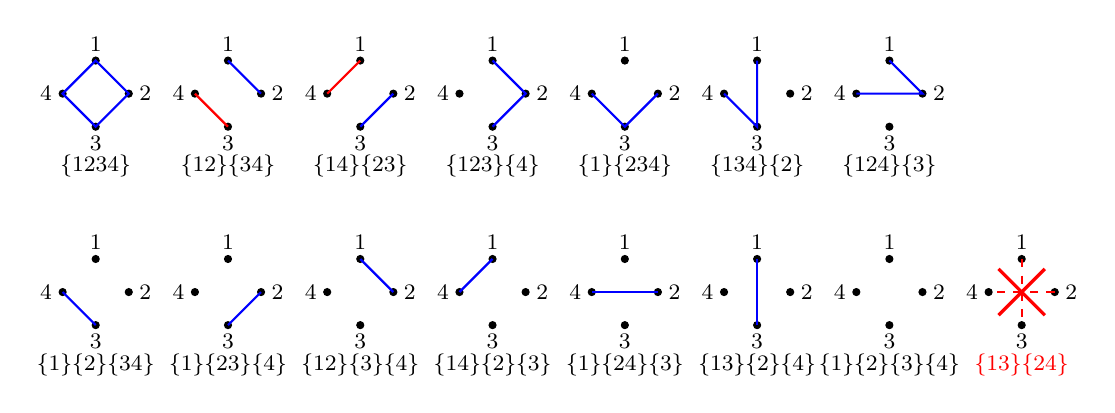
\begin{tikzpicture}[scale=0.42, every node/.style={font=\footnotesize}]

  \begin{scope}[shift={(0,0)}]
    \foreach \i/\a in {1/90, 2/0, 3/270, 4/180} {
      \filldraw (\a:1) circle (3pt);
      \node at (\a:1.5) {\i};
    }
    \draw[thick, blue] (90:1) -- (0:1) -- (270:1) -- (180:1) -- cycle;
    \node at (0,-2.2) {$\{1234\}$};
  \end{scope}

  \begin{scope}[shift={(4,0)}]
    \foreach \i/\a in {1/90, 2/0, 3/270, 4/180} {
      \filldraw (\a:1) circle (3pt);
      \node at (\a:1.5) {\i};
    }
    \draw[thick, blue] (90:1) -- (0:1);
    \draw[thick, red] (270:1) -- (180:1);
    \node at (0,-2.2) {$\{12\}\{34\}$};
  \end{scope}

  \begin{scope}[shift={(8,0)}]
    \foreach \i/\a in {1/90, 2/0, 3/270, 4/180} {
      \filldraw (\a:1) circle (3pt);
      \node at (\a:1.5) {\i};
    }
    \draw[thick, blue] (0:1) -- (270:1);
    \draw[thick, red] (90:1) -- (180:1);
    \node at (0,-2.2) {$\{14\}\{23\}$};
  \end{scope}

  \begin{scope}[shift={(12,0)}]
    \foreach \i/\a in {1/90, 2/0, 3/270, 4/180} {
      \filldraw (\a:1) circle (3pt);
      \node at (\a:1.5) {\i};
    }
    \draw[thick, blue] (90:1) -- (0:1) -- (270:1);
    \draw[thick, red] (180:1) circle (0pt);
    \node at (0,-2.2) {$\{123\}\{4\}$};
  \end{scope}

  \begin{scope}[shift={(16,0)}]
    \foreach \i/\a in {1/90, 2/0, 3/270, 4/180} {
      \filldraw (\a:1) circle (3pt);
      \node at (\a:1.5) {\i};
    }
    \draw[thick, blue] (0:1) -- (270:1) -- (180:1);
    \draw[thick, red] (90:1) circle (0pt);
    \node at (0,-2.2) {$\{1\}\{234\}$};
  \end{scope}

  \begin{scope}[shift={(20,0)}]
    \foreach \i/\a in {1/90, 2/0, 3/270, 4/180} {
      \filldraw (\a:1) circle (3pt);
      \node at (\a:1.5) {\i};
    }
    \draw[thick, blue] (90:1) -- (270:1) -- (180:1);
    \draw[thick, red] (0:1) circle (0pt);
    \node at (0,-2.2) {$\{134\}\{2\}$};
  \end{scope}

  \begin{scope}[shift={(24,0)}]
    \foreach \i/\a in {1/90, 2/0, 3/270, 4/180} {
      \filldraw (\a:1) circle (3pt);
      \node at (\a:1.5) {\i};
    }
    \draw[thick, blue] (90:1) -- (0:1) -- (180:1);
    \draw[thick, red] (270:1) circle (0pt);
    \node at (0,-2.2) {$\{124\}\{3\}$};
  \end{scope}

  \begin{scope}[shift={(0,-6)}]
    \foreach \i/\a in {1/90, 2/0, 3/270, 4/180} {
      \filldraw (\a:1) circle (3pt);
      \node at (\a:1.5) {\i};
    }
    \draw[thick, blue] (270:1) -- (180:1);
    \node at (0,-2.2) {$\{1\}\{2\}\{34\}$};
  \end{scope}

  \begin{scope}[shift={(4,-6)}]
    \foreach \i/\a in {1/90, 2/0, 3/270, 4/180} {
      \filldraw (\a:1) circle (3pt);
      \node at (\a:1.5) {\i};
    }
    \draw[thick, blue] (0:1) -- (270:1);
    \node at (0,-2.2) {$\{1\}\{23\}\{4\}$};
  \end{scope}

  \begin{scope}[shift={(8,-6)}]
    \foreach \i/\a in {1/90, 2/0, 3/270, 4/180} {
      \filldraw (\a:1) circle (3pt);
      \node at (\a:1.5) {\i};
    }
    \draw[thick, blue] (90:1) -- (0:1);
    \node at (0,-2.2) {$\{12\}\{3\}\{4\}$};
  \end{scope}

  \begin{scope}[shift={(12,-6)}]
    \foreach \i/\a in {1/90, 2/0, 3/270, 4/180} {
      \filldraw (\a:1) circle (3pt);
      \node at (\a:1.5) {\i};
    }
    \draw[thick, blue] (90:1) -- (180:1);
    \node at (0,-2.2) {$\{14\}\{2\}\{3\}$};
  \end{scope}

  \begin{scope}[shift={(16,-6)}]
    \foreach \i/\a in {1/90, 2/0, 3/270, 4/180} {
      \filldraw (\a:1) circle (3pt);
      \node at (\a:1.5) {\i};
    }
    \draw[thick, blue] (0:1) -- (180:1);
    \node at (0,-2.2) {$\{1\}\{24\}\{3\}$};
  \end{scope}

  \begin{scope}[shift={(20,-6)}]
    \foreach \i/\a in {1/90, 2/0, 3/270, 4/180} {
      \filldraw (\a:1) circle (3pt);
      \node at (\a:1.5) {\i};
    }
    \draw[thick, blue] (90:1) -- (270:1);
    \node at (0,-2.2) {$\{13\}\{2\}\{4\}$};
  \end{scope}

  \begin{scope}[shift={(24,-6)}]
    \foreach \i/\a in {1/90, 2/0, 3/270, 4/180} {
      \filldraw (\a:1) circle (3pt);
      \node at (\a:1.5) {\i};
    }
    \node at (0,-2.2) {$\{1\}\{2\}\{3\}\{4\}$};
  \end{scope}

  \begin{scope}[shift={(28,-6)}]
    \foreach \i/\a in {1/90, 2/0, 3/270, 4/180} {
      \filldraw (\a:1) circle (3pt);
      \node at (\a:1.5) {\i};
    }
    \draw[thick, red, dashed] (0:1) -- (180:1);
    \draw[thick, red, dashed] (90:1) -- (270:1);
    \node[red] at (0,-2.2) {$\{13\}\{24\}$};
    \draw[red, very thick] (-0.7,-0.7) -- (0.7,0.7);
    \draw[red, very thick] (0.7,-0.7) -- (-0.7,0.7);
  \end{scope}

\end{tikzpicture}
\end{adjustbox}
\caption{Non-crossing partitions of $\{1,2,3,4\}$, arranged on circles.
  All $C_4 = 14$ non-crossing partitions are shown.  The sole crossing
  partition $\{\{1,3\},\{2,4\}\}$ is displayed last with dashed red arcs
  and an ``X'' to indicate that it is excluded from $\mathrm{NC}(4)$.
  In the planar flat-weight replica model used here, these partitions label
  replica contraction patterns; each block labels a connected replica component.}
\label{fig07:nc_partitions}
\end{figure}


\paragraph{Catalan numbers.}
The number of non-crossing partitions of $\{1,\ldots,n\}$ is the $n$-th
Catalan number,
\begin{equation}
  C_n \;=\; \frac{1}{n+1}\binom{2n}{n},
  \label{eq07:catalan}
\end{equation}
with values $C_0 = 1$, $C_1 = 1$, $C_2 = 2$, $C_3 = 5$, $C_4 = 14$,
$C_5 = 42$, $C_6 = 132$.  The Catalan numbers grow asymptotically as
$C_n \sim 4^n / (n^{3/2}\sqrt{\pi})$, which is substantially slower than
the Bell numbers $B_n$ counting all partitions.  The restriction to
non-crossing partitions thus represents a dramatic simplification of the
combinatorial structure.

\paragraph{Narayana numbers.}
A finer invariant of a non-crossing partition is its number of blocks.
The number of non-crossing partitions of $\{1,\ldots,n\}$ with exactly
$j$ blocks is the \emph{Narayana number}
\begin{equation}
  N(n,j) \;=\; \frac{1}{n}\binom{n}{j}\binom{n}{j-1}.
  \label{eq07:narayana}
\end{equation}
The Narayana numbers refine the Catalan numbers:
$\sum_{j=1}^{n} N(n,j) = C_n$.  They satisfy the symmetry
\begin{equation}
  N(n,j) = N(n, n+1-j),
  \label{eq07:narayana_symmetry}
\end{equation}
reflecting a duality between a partition and its Kreweras
complement \cite{kreweras1972}.

Table~\ref{tab07:narayana} lists the Narayana numbers for small $n$.

\begin{table}[t]
\centering
\caption{Narayana numbers $N(n,j)$: the number of non-crossing partitions
  of $\{1,\ldots,n\}$ with exactly $j$ blocks.  Row sums give the Catalan
  numbers $C_n$. In the planar flat-weight replica model used here, $j$
  counts the connected replica components of the contraction pattern.}
\label{tab07:narayana}
\medskip
\begin{adjustbox}{max width=\textwidth,center}
\begin{tabular}{c|ccccc|c}
\toprule
$n \backslash j$ & 1 & 2 & 3 & 4 & 5 & $C_n$ \\
\midrule
2 & 1 & 1 & & & & 2 \\
3 & 1 & 3 & 1 & & & 5 \\
4 & 1 & 6 & 6 & 1 & & 14 \\
5 & 1 & 10 & 20 & 10 & 1 & 42 \\
\bottomrule
\end{tabular}
\end{adjustbox}
\end{table}

\paragraph{Gravitational interpretation.}
In the planar flat-weight replica model, a non-crossing partition of
$\{1,\ldots,n\}$ with $j$ blocks labels a contraction pattern with $j$
connected replica components. The west-coast interpretation associates a
connected component with a gravitational amplitude joining the corresponding
replicas. The Narayana number $N(n,j)$ counts these contraction patterns.
It does not enumerate every geometry or saddle that may contribute to a
gravitational amplitude with those boundary data.


\subsection{Free cumulants and the moment-cumulant relation}
\label{subsec07:free_cumulants}

We now make the free-probability structure precise.  Recall the
moment-cumulant relation \eqref{eq07:free_moment_cumulant}:
\begin{equation}
  M_n = \sum_{\pi \in \mathrm{NC}(n)} \prod_{B \in \pi} \kappa_{|B|}.
  \label{eq07:free_mc_repeat}
\end{equation}
This relation defines the free cumulants $\kappa_m$ recursively from the
moments $M_n$, or vice versa.  The first few relations are:
\begin{align}
  M_1 &= \kappa_1, \label{eq07:mc1} \\
  M_2 &= \kappa_2 + \kappa_1^2, \label{eq07:mc2} \\
  M_3 &= \kappa_3 + 3\kappa_2\kappa_1 + \kappa_1^3, \label{eq07:mc3} \\
  M_4 &= \kappa_4 + 4\kappa_3\kappa_1 + 2\kappa_2^2
        + 6\kappa_2\kappa_1^2 + \kappa_1^4. \label{eq07:mc4}
\end{align}
The coefficients in these expressions are precisely the Narayana numbers
from Table~\ref{tab07:narayana}: for $M_4$, the terms with one block
($\kappa_4$) appear $N(4,1)=1$ time, those with two blocks
($\kappa_3\kappa_1$ and $\kappa_2^2$) appear a total of $N(4,2)=6$
times, and so on.

\paragraph{Classical comparison.}
The classical moment-cumulant relation has the same form but sums over
\emph{all} partitions $\mathcal{P}(n)$.  For instance, the classical
relation for $M_4$ includes an additional term from the crossing partition
$\{\{1,3\},\{2,4\}\}$:
\begin{equation}
  M_4^{\text{classical}} = \chi_4 + 4\chi_3 \chi_1 + 3\chi_2^2 + 6\chi_2 \chi_1^2
  + \chi_1^4,
  \label{eq07:classical_m4}
\end{equation}
where the coefficient of $\chi_2^2$ is 3 (from the three partitions into
two pairs) rather than 2.  The single additional contribution comes from
the crossing partition $\{\{1,3\},\{2,4\}\}$.

\paragraph{Free cumulants of the flat-weight model.}
The Narayana moment formula of Section~\ref{sec06:replica_wormholes} is
reproduced by the free cumulants
\begin{equation}
  \boxed{
    \kappa_m = \gamma^{m-1}, \qquad \gamma = \frac{k}{L},
  }
  \label{eq07:gravity_cumulants}
\end{equation}
where $k$ is the dimension of the radiation Hilbert space and $L$ is the
dimension of the black hole interior Hilbert space.  The ratio $\gamma$ compares the two dimensions.  Calling its crossing of
one a Page time additionally requires a specified time-dependent preparation.

The identification~\eqref{eq07:gravity_cumulants} is the central
quantitative result of the genus-zero analysis.  The free cumulants
$\kappa_m = \gamma^{m-1}$ are precisely those of the \emph{free Poisson
distribution}, also known as the \emph{Marchenko--Pastur distribution}.
We shall derive this distribution explicitly in
Section~\ref{subsec07:marchenko_pastur}.


\subsection{The \texorpdfstring{$R$}{R}-transform}
\label{subsec07:r_transform}

Free probability provides a generating-function technology, the
$R$-transform, that packages the free cumulants into an analytic function
and plays the role of the logarithm of the moment generating function in
classical probability.

\paragraph{Definition.}
The $R$-transform is the generating function of the free cumulants:
\begin{equation}
  R(z) = \sum_{m=1}^{\infty} \kappa_m\, z^{m-1}.
  \label{eq07:r_transform_def}
\end{equation}
For the flat-weight free cumulants \eqref{eq07:gravity_cumulants}, this
becomes a geometric series:
\begin{equation}
  \boxed{
    R(z) = \sum_{m=1}^{\infty} \gamma^{m-1} z^{m-1}
         = \frac{1}{1 - \gamma z}.
  }
  \label{eq07:r_gravity}
\end{equation}

\paragraph{Free convolution.}
The key property of the $R$-transform is its behavior under
\emph{free convolution} $\boxplus$: if $X$ and $Y$ are freely independent,
then
\begin{equation}
  R_{X+Y}(z) = R_X(z) + R_Y(z).
  \label{eq07:free_convolution}
\end{equation}
This is the free-probability analogue of the fact that the log-MGF
(cumulant generating function) is additive under classical convolution.
Free convolution describes limiting eigenvalue distributions of sums when
the matrices are asymptotically free, as in suitable independent
unitarily invariant ensembles. Classical independence of matrix entries or
of the two matrices alone is insufficient. The additivity of $R$ makes
it useful once the freeness hypotheses hold.

\paragraph{From $R$-transform to spectral density.}
The $R$-transform determines the Cauchy (or Stieltjes) transform $G(z)$
of the eigenvalue density through the functional equation
\begin{equation}
  G\!\bigl(R(z) + 1/z\bigr) = z.
  \label{eq07:g_from_r}
\end{equation}
Here $G(z)$ is defined as
\begin{equation}
  G(z) = \int \frac{f(\lambda)}{z - \lambda}\, d\lambda,
  \label{eq07:cauchy_transform}
\end{equation}
where $f(\lambda)$ is the eigenvalue density.  The density is recovered by
the Stieltjes inversion formula:
\begin{equation}
  f(\lambda) = -\frac{1}{\pi}
    \lim_{\epsilon \to 0^+} \operatorname{Im}\, G(\lambda + i\epsilon).
  \label{eq07:stieltjes_inversion}
\end{equation}

For the gravitational $R$-transform \eqref{eq07:r_gravity}, substituting
$R(z) = 1/(1-\gamma z)$ into \eqref{eq07:g_from_r} and solving for
$G(z)$ yields a quadratic equation whose solution gives the
Marchenko--Pastur distribution, as we now derive.


\subsection{The Marchenko--Pastur distribution}
\label{subsec07:marchenko_pastur}

\paragraph{Derivation from the $R$-transform.}
We seek the spectral density $f(\lambda)$ corresponding to the
$R$-transform $R(z) = 1/(1-\gamma z)$.  The functional equation
\eqref{eq07:g_from_r} states that $G$ inverts the map
$z \mapsto R(z) + 1/z$; evaluating that map at $z = G(w)$ must therefore
return $w$:
\begin{equation}
  w = \frac{1}{1-\gamma G(w)} + \frac{1}{G(w)}.
  \label{eq07:w_eq}
\end{equation}
Multiplying through by $G(1-\gamma G)$ and collecting terms yields a
quadratic equation for $G = G(w)$:
\begin{equation}
  \gamma w\, G^2 - (w + \gamma - 1)\, G + 1 = 0.
  \label{eq07:quadratic_z}
\end{equation}
The discriminant factorizes as
$(w + \gamma - 1)^2 - 4\gamma w = (w - a_+)(w - a_-)$, where
\begin{equation}
  a_{\pm} = (1 \pm \sqrt{\gamma})^2,
  \label{eq07:mp_edges}
\end{equation}
and the quadratic formula gives
\begin{equation}
  G(w) = \frac{(w + \gamma - 1)
    - \sqrt{(w - a_+)(w - a_-)}}{2\gamma w},
  \label{eq07:cauchy_mp}
\end{equation}
where the branch of the square root is chosen so that
$G(w) \sim 1/w$ as $w \to \infty$.

For $\lambda \in [a_-, a_+]$, the square root in \eqref{eq07:cauchy_mp}
becomes purely imaginary, and the Stieltjes inversion formula
\eqref{eq07:stieltjes_inversion} gives the Marchenko--Pastur density:
\begin{equation}
  \boxed{
    f_{\mathrm{MP}}(\lambda; \gamma)
    = \frac{\sqrt{(a_+ - \lambda)(\lambda - a_-)}}{2\pi \gamma \lambda},
    \qquad \lambda \in [a_-, a_+].
  }
  \label{eq07:mp_density}
\end{equation}
For $\gamma > 1$, the density is supplemented by a point mass at the
origin:
\begin{equation}
  f(\lambda; \gamma)
  = \Bigl(1 - \frac{1}{\gamma}\Bigr)\,\delta(\lambda)
  + f_{\mathrm{MP}}(\lambda;\gamma),
  \qquad \gamma > 1.
  \label{eq07:mp_point_mass}
\end{equation}
The point mass corresponds to the $k - L$ exactly zero eigenvalues of the
reduced density matrix when the radiation Hilbert space is larger than the
black hole interior.

\begin{figure}[t]
  \centering
  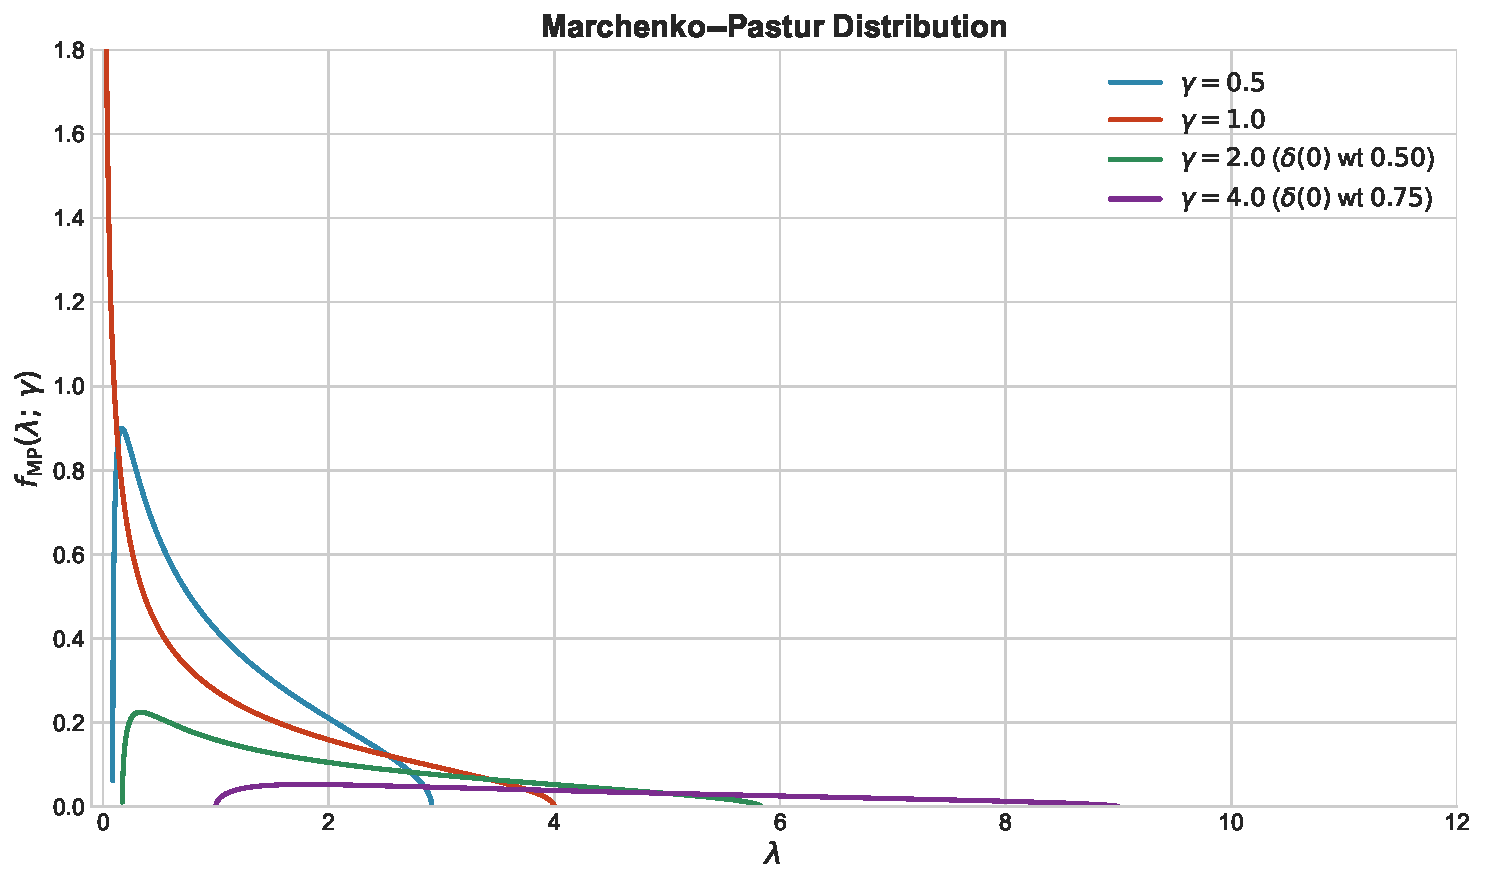
\includegraphics[width=0.85\textwidth]{figures/output/fig07_marchenko_pastur.pdf}
  \caption{The Marchenko--Pastur density
    $f_{\mathrm{MP}}(\lambda;\gamma)$ for
    $\gamma = 0.5, 1, 2, 4$.  As $\gamma$ increases, the support
    widens and shifts rightward.  For every $\gamma \neq 1$ the density
    vanishes like a square root at both edges.  For $\gamma > 1$, the
    lower edge $a_- = (1-\sqrt{\gamma})^2$ remains positive and a point
    mass of weight $(1 - 1/\gamma)$ appears at $\lambda = 0$
    (Eq.~\eqref{eq07:mp_point_mass}).
    At the dimension crossing $\gamma=1$, the lower edge touches zero
    ($a_- = 0$, $a_+ = 4$) and the density diverges as
    $\lambda^{-1/2}$ at the origin.}
  \label{fig07:marchenko_pastur}
\end{figure}

\paragraph{Physical interpretation.}
For a Haar-random pure state in $\mathbb C^k\otimes\mathbb C^L$, the
empirical distribution of the rescaled radiation eigenvalues $k\lambda_i$
converges to this law as $k,L\to\infty$ at fixed $\gamma=k/L$.  The same
law follows for the planar flat-weight replica model
\cite{pssyetal2022}.  Equality of this limiting density establishes equality
of the corresponding limiting linear spectral statistics, subject to the
integrability needed by the observable.  It does not establish equality of
finite-dimensional joint eigenvalue distributions, connected ensemble
fluctuations, eigenvectors, or evaporation channels.

Marchenko--Pastur distributions also occur for specified Gram matrices of
black-hole microstate families~\cite{muck2024,balasubramanianetal2024}.
Those Gram matrices and radiation density matrices are distinct operators;
their common limiting law must be derived for each preparation.

\paragraph{Special cases.}
\begin{itemize}
  \item \textbf{At equal dimensions} ($\gamma = 1$): the support is
    $[0, 4]$, and the density simplifies to
    \begin{equation}
      f_{\mathrm{MP}}(\lambda; 1)
      = \frac{\sqrt{4 - \lambda}}{2\pi\sqrt{\lambda}},
      \qquad \lambda \in [0, 4].
      \label{eq07:mp_page_time}
    \end{equation}
    This is the quarter-circle law (up to a change of variables), the
    iconic distribution of random matrix theory.

  \item \textbf{Early time} ($\gamma \ll 1$): in the scaled variable of
    $f_{\mathrm{MP}}$, the mass concentrates near $\lambda = 1$ (the
    support $[a_-, a_+]$ shrinks around $1$).  The physical eigenvalues
    of $\rho_{\mathrm{rad}}$ carry an additional normalization factor
    of $1/k$, so they cluster near $1/k$: a nearly maximally mixed
    state of the radiation.

  \item \textbf{Late time} ($\gamma \gg 1$): most eigenvalues are zero
    (the point mass dominates), and the nonzero part of the scaled
    density concentrates near $\lambda = \gamma$.  In physical terms,
    the $L$ nonzero eigenvalues cluster near $\gamma/k = 1/L$,
    giving entropy close to $\log L$.  This becomes a nearly pure state only
    when the remaining factor itself has dimension near one.
\end{itemize}

\paragraph{Entropy from the density.}
For entropy it is convenient to use the smaller subsystem.  Set
$m=\min(k,L)$, $b=\max(k,L)$, and introduce the separate ratio
$\eta=m/b\leq1$; the raw ratio remains $\gamma=k/L$.
Let $\lambda$ now denote $m$ times a nonzero eigenvalue.  Its limiting law is
$\mathrm{MP}(\eta)$, with edges $(1\pm\sqrt\eta)^2$.  No entropy information
is lost, because
for a pure global state the nonzero spectra of the two reduced density
matrices coincide, so all spectral quantities are symmetric under
$k \leftrightarrow L$.  The leading large-dimension von~Neumann entropy is then
\begin{equation}
  S_{\mathrm{MP}}
  = \log\min(k,L)
  - \int_{a_-}^{a_+} f_{\mathrm{MP}}(\lambda;\eta)\,
    \lambda \log \lambda \; d\lambda,
  \label{eq07:entropy_integral}
\end{equation}
where the first term restores the eigenvalue normalization: writing
$\lambda_{\mathrm{phys}} = \lambda/\min(k,L)$ and using
$\int f_{\mathrm{MP}}\,\lambda\,d\lambda = M_1 = 1$, the sum
$-\sum \lambda_{\mathrm{phys}} \log \lambda_{\mathrm{phys}}$ splits
into exactly these two terms.  The integral evaluates in closed form to
$\eta/2$; the result is the west-coast scaling function discussed in
Section~\ref{subsec07:penington_scaling}, consistent with
Eq.~\eqref{eq07:penington_entropy} below.

For an explicit evaluation, set
$\lambda=1+\eta-2\sqrt\eta\cos\theta$, $0\leq\theta\leq\pi$.
Then
\begin{equation}
 \int\lambda\log\lambda\,f_{\mathrm{MP}}(\lambda;\eta)\,d\lambda
 =\frac2\pi\int_0^\pi\sin^2\theta\,
 \log(1+\eta-2\sqrt\eta\cos\theta)\,d\theta.
 \label{eq07:entropy_angle}
\end{equation}
For $0<\eta<1$, expand the logarithm as
$-2\sum_{j\geq1}\eta^{j/2}\cos(j\theta)/j$.
Orthogonality with $\sin^2\theta=(1-\cos2\theta)/2$ removes every term
except $j=2$, whose integral gives $\eta/2$.  The endpoint $\eta=1$
follows by integrability and passage to the limit.  This derivation computes
the constant deficit directly from the limiting spectrum.


\subsection{Analytic continuation: Carlson's theorem}
\label{subsec07:carlson}

The replica trick computes $\operatorname{Tr}(\rho^n)$ for integer
$n \geq 2$ and then analytically continues to $n \to 1$ to extract the
von~Neumann entropy via
\begin{equation}
  S_{\mathrm{vN}} = -\lim_{n \to 1}
    \frac{\partial}{\partial n}\operatorname{Tr}(\rho^n).
  \label{eq07:replica_limit}
\end{equation}
But analytic continuation from the integers is not unique in general ---
one can always add a function that vanishes at all positive integers (for
instance, $\sin(\pi n)$ times any bounded function).  A natural question
is: \emph{what justifies the specific analytic continuation given by the
Marchenko--Pastur moment formula?}

The answer is provided by Carlson's theorem \cite{carlson1914}:

\begin{quote}
\textbf{Carlson's Theorem.}\quad
Let $f(z)$ be holomorphic in the right half-plane
$\operatorname{Re}(z) > 0$, and suppose:
\begin{enumerate}
  \item[(i)] $f(n) = 0$ for all positive integers $n$;
  \item[(ii)] $|f(z)| \leq C e^{c|z|}$ for some constants $C, c$ with
    $c < \pi$.
\end{enumerate}
Then $f(z) \equiv 0$.
\end{quote}

The theorem implies that if two holomorphic functions agree at all
positive integers and both satisfy the exponential growth bound with
$c < \pi$, they must be identical.  Thus, to justify the replica limit,
one must verify that the Marchenko--Pastur moment formula
\begin{equation}
  M_n(\eta)
  = \int_{a_-}^{a_+} \lambda^n \, f_{\mathrm{MP}}(\lambda;\eta)\, d\lambda,
  \qquad
  \mathbb E_{\mathrm H}\operatorname{Tr}(\rho^n)\sim m^{1-n}M_n(\eta),
  \label{eq07:mp_moments}
\end{equation}
satisfies the growth bound.  The continuation is performed on the
scaled moments $M_n(\eta)$; the prefactor $\min(k,L)^{1-n}$ is an
explicit elementary function of $n$ and requires no interpolation.

For a complex index $z$ with $\operatorname{Re}z>0$, the compact support
gives $|M_z(\eta)|\leq a_+^{\operatorname{Re}z}\leq e^{|z|\log a_+}$.
For real $n>0$ this reads
\begin{equation}
  |M_n(\eta)| \leq a_+^n = \bigl[(1+\sqrt{\eta})^2\bigr]^n,
  \label{eq07:moment_bound}
\end{equation}
so the exponential growth rate is
\begin{equation}
  c = \log a_+ = 2\log(1+\sqrt{\eta}).
  \label{eq07:growth_rate}
\end{equation}
Since $0<\eta\leq1$, the required bound is
\begin{equation}
 c=2\log(1+\sqrt\eta)\leq\log4<\pi.
 \label{eq07:carlson_bound}
\end{equation}
Thus the moment integral has the required half-plane growth.  At the lower
edge zero, its derivative near $z=1$ remains integrable because
$\lambda\log\lambda\,f_{\mathrm{MP}}(\lambda;1)$ is integrable.
An alternative, purely spectral justification is compact moment
determinacy: polynomials are dense in the continuous functions on
$[0,a_+]$, so all integer moments uniquely determine the measure.  The
entropy then follows by integration against that measure.

Within the stated bounded-exponential-growth class, the
Marchenko--Pastur moment integral \eqref{eq07:mp_moments} is the
\emph{unique} analytic continuation of the scaled planar moments
$M_n(\eta)$ from integer $n$ to real $n$, and the replica limit
$n \to 1$ is thereby justified.


\subsection{The west-coast scaling function}
\label{subsec07:penington_scaling}

We now have all the ingredients to extract the von~Neumann entropy from
the Marchenko--Pastur distribution.  The result is the
\emph{west-coast scaling function}, which gives the planar entropy correction in the flat-weight model.
It is the large-dimension limit of Page's mean-entropy formula
\cite{page1993}, rather than the exact finite-dimensional mean entropy.

\paragraph{The result.}
Define the dimensionless parameter
\begin{equation}
  \Delta = \log\gamma = \log\frac{k}{L},
  \label{eq07:delta_def}
\end{equation}
which measures the logarithmic distance from the dimension crossing ($\Delta = 0$
when $k = L$).  The von~Neumann entropy of the radiation, computed from
the Marchenko--Pastur distribution, takes the form
\begin{equation}
  \boxed{
    S_{\mathrm{MP}} = \log\min(k, L) + F(\Delta),
  }
  \label{eq07:penington_entropy}
\end{equation}
where the \emph{west-coast scaling function} is
\begin{equation}
  \boxed{
    F(\Delta) = -\frac{1}{2}\, e^{-|\Delta|}.
  }
  \label{eq07:penington_f}
\end{equation}

\begin{figure}[t]
  \centering
  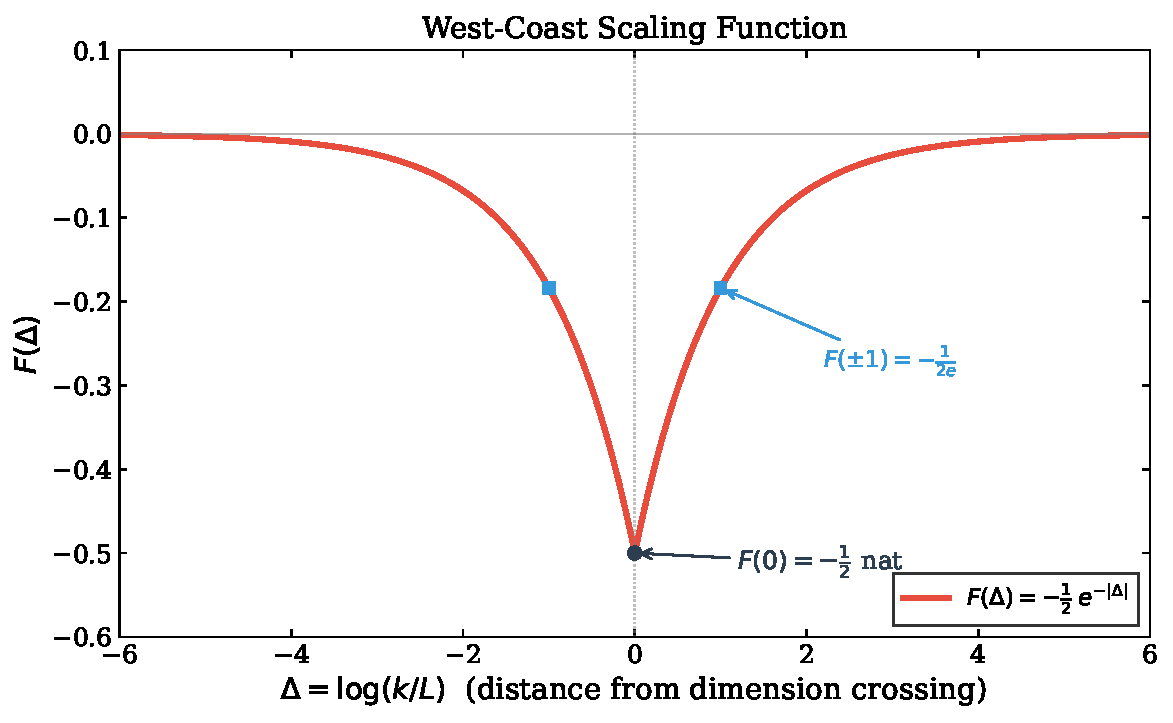
\includegraphics[width=0.85\textwidth]{figures/output/fig07_westcoast_scaling.pdf}
  \caption{The west-coast scaling function $F(\Delta)$, where
    $\Delta = \log(k/L)$ measures the logarithmic distance from equal dimensions.
    The function reaches its minimum $F(0) = -1/2$ nat at $k=L$ and decays exponentially on both sides with $e$-folding
    scale $|\Delta| = 1$.  The entire transition region has width
    $O(1)$ in $\Delta$, corresponding to $O(1)$ in $\log(k/L)$.}
  \label{fig07:penington_scaling}
\end{figure}

\paragraph{Properties.}
The west-coast scaling function has several notable features:
\begin{enumerate}
  \item \textbf{Peak deficit}: $F(0) = -1/2$ nat.  At the Page time,
    the entropy falls short of $\log\min(k,L) = \log k = \log L$ by
    exactly $1/2$ nat.  This is the genus-zero analogue of the
    $O(1)$ correction computed by Page \cite{page1993}.

  \item \textbf{Transition width}: The function decays as
    $e^{-|\Delta|}$, so the transition from ``before Page time'' to
    ``after Page time'' occurs over a window of width $O(1)$ in
    $\Delta = \log(k/L)$.  This is an order-one window in the entropy difference, hence a relative
    width that vanishes when compared with a macroscopic entropy scale.

  \item \textbf{Exponential tails}: For $|\Delta| \gg 1$,
    $F(\Delta) \to 0$ exponentially fast.  Far from the Page time, the
    entropy is well approximated by the sharp Page curve
    $\log\min(k,L)$.

  \item \textbf{Symmetry}: $F(\Delta) = F(-\Delta)$.  This reflects the
    Narayana symmetry $N(n,j) = N(n,n+1-j)$ and, physically, the
    duality between radiation and black hole interior in the genus-zero
    sector.
\end{enumerate}

\paragraph{The smooth Page curve.}
Combining \eqref{eq07:penington_entropy} and \eqref{eq07:penington_f},
the flat-weight planar entropy is
\begin{equation}
  S_{\mathrm{MP}}
  = \min\bigl(S_{\mathrm{rad}},\, S_{\mathrm{BH}}\bigr)
    - \frac{1}{2}\, e^{-|\Delta|},
  \label{eq07:smooth_page_curve}
\end{equation}
where $S_{\mathrm{rad}} = \log k$ and $S_{\mathrm{BH}} = \log L$ are
the coarse-grained entropies.  This replaces the sharp
$\min(S_{\mathrm{rad}}, S_{\mathrm{BH}})$ of the idealized Page curve
with a function whose first two derivatives match at $\Delta=0$ when
the branch mean is varied smoothly.  The local rounding is quadratic, but
this planar function need not be analytic to all orders at the crossing.
At fixed $L$ the curve rises and saturates; a falling branch additionally
requires a decreasing black-hole dimension or another specified evolution.

\begin{figure}[t]
  \centering
  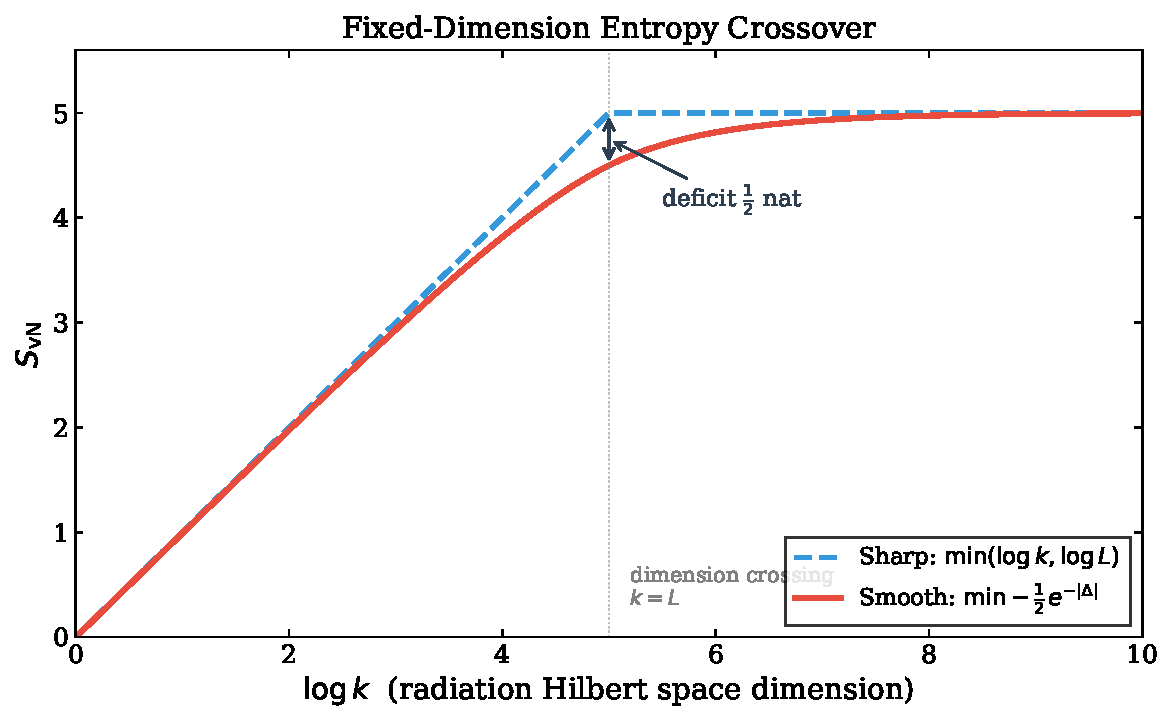
\includegraphics[width=0.85\textwidth]{figures/output/fig07_sharp_vs_smooth.pdf}
  \caption{The fixed-$L$ scan: comparison of the sharp dimension bound
    $\min(\log k, \log L)$ (dashed blue) with the smooth genus-zero
    Page curve $\min(\log k, \log L) - \frac{1}{2}e^{-|\Delta|}$
    (solid red), where $\Delta = \log(k/L)$.  The west-coast scaling
    function resolves the cusp at equal dimensions into a smooth transition.
    The maximum deficit is $1/2$ nat at $k=L$. This is a dimension scan;
    a time profile requires a dynamical preparation.}
  \label{fig07:sharp_vs_smooth}
\end{figure}

\paragraph{Finite dimensions and the scope of the limit.}
For $m=\min(k,L)$ and $b=\max(k,L)$, the exact Haar mean entropy is
\begin{equation}
 \mathbb E_{\mathrm H}S(\rho)=H_{mb}-H_b-\frac{m-1}{2b},
 \qquad H_j=\sum_{r=1}^j\frac1r.
 \label{eq07:finite_page}
\end{equation}
This is Page's result~\cite{page1993,sen1996}.  Using
$H_j=\log j+\gamma_{\!E}+1/(2j)-1/(12j^2)+O(j^{-4})$ gives
\begin{equation}
 \mathbb E_{\mathrm H}S(\rho)
 =\log m-\frac{m}{2b}
 +\frac{1}{2mb}+\frac{1}{12b^2}
 -\frac{1}{12m^2b^2}+O(b^{-4}),
 \label{eq07:page_expansion}
\end{equation}
with both dimensions large at fixed positive $m/b$.
The leading correction to the Marchenko--Pastur entropy is therefore of
order $b^{-2}$ in this regime.  At $m=b=L$ it is $7/(12L^2)$.
For $m=b=2$, the exact entropy is $1/3$ nat, whereas the planar expression is
$\log2-1/2\simeq0.1931$ nat.  Small dimensions should be evaluated by the
exact formula.

Other ensembles can have the same limiting density but different finite-size
corrections or connected fluctuations.  Weak convergence alone also needs
supplementing by suitable tail control to pass to an unbounded spectral
observable.  The Gaussian/Haar benchmark supplies this control; the same
conclusion for a gravitational preparation requires its own spectral analysis.

\paragraph{Summary.}
Flat cycle weights give the free cumulants $\kappa_m=\gamma^{m-1}$.
Their $R$-transform determines the Marchenko--Pastur density, whose smaller-side
form has ratio $\eta=\min(k,L)/\max(k,L)$.  Integrating that density gives
$S_{\mathrm{MP}}=\log\min(k,L)-\eta/2$.  The exact finite Haar answer has
additional normalization and spectral corrections.  General planar replica
models use the same non-crossing organization with their own cycle weights.

\part{Thermodynamic Fluctuations and Entropy Transitions}

\section{Entropy Averages and Gaussian Fluctuations}
\label{sec08:area_fluctuations}

The fixed-dimension Page calculation describes a random pure state on a tensor
product whose dimensions are specified. Thermodynamic preparations introduce a
second source of variation: the number and weights of accessible states depend
on energy. Averaging over that variation can round the leading minimum of two
entropy branches on a scale larger than the order-one Page correction. Before
performing the average, however, one must identify the random variable and the
quantum state whose entropy is sought.

Enhanced corrections of this kind occur in chaotic energy eigenstates
\citep{vidmarrigol2017,murthysrednicki2019}. In gravity, the diagonal
approximation of \citet{marolfwangwang2020} averages fixed-area entropies, and
\citet{dongwang2020} obtained enhanced corrections by summing replica saddles
in a chaotic holographic example. The Gaussian minimum formula derived below
is established material from this literature. Its elementary derivation is
included because it makes both the mechanism and the approximation explicit.
Paper~I \citep{wuebben2026paper1} compares a specified level-resolved diagonal
approximation with the planar spectrum; Paper~II
\citep{wuebben2026paper2} studies regular and critical thermodynamic
fluctuations within a canonical random-state model.

\subsection{The fluctuating entropy difference}
\label{subsec08:why_area_fluctuates}

Let $F_1$ and $F_2$ be integrable random variables representing two candidate
entropy branches. The exact identity
\begin{equation}
 \mathbb E\min(F_1,F_2)
 =\frac{\mathbb EF_1+\mathbb EF_2}{2}
  -\frac12\mathbb E|F_1-F_2|
 \label{eq08:branch_identity}
\end{equation}
shows which fluctuations matter. The deficit relative to the minimum of the
mean branches is
\begin{equation}
 B=\frac12\left(\mathbb E|F_1-F_2|
             -|\mathbb EF_1-\mathbb EF_2|\right)\geq0.
 \label{eq08:branch_deficit}
\end{equation}
The inequality follows from convexity of the absolute value. In particular,
\begin{equation}
 \sigma_{\mathrm{gap}}^2
 =\operatorname{Var}F_1+\operatorname{Var}F_2
  -2\operatorname{Cov}(F_1,F_2).
 \label{eq08:gap_variance}
\end{equation}
A fluctuation shared equally by both branches cancels from their difference.
A thermodynamic heat capacity therefore becomes an entropy-transition width
only after the response of both branches has been specified. This point will
be important for a finite reservoir in Section~\ref{sec09:higher_dimensions}.

For example, if $F_1=s$ is deterministic and $F_2=Y$ is random with mean $\mu$,
write $\Delta=s-\mu$ and $\xi=Y-\mu$. Then
\begin{equation}
 M(\Delta)=\mathbb E\min(\Delta,\xi),\qquad
 B(\Delta)=\min(\Delta,0)-M(\Delta)
 =\frac12\left(\mathbb E|\Delta-\xi|-|\Delta|\right).
 \label{eq08:general_minimum}
\end{equation}
At the crossing of the mean branches,
\begin{equation}
 B(0)=\frac12\mathbb E|\xi|\leq\frac12\sigma,
 \qquad \sigma^2=\mathbb E\xi^2.
 \label{eq08:general_midpoint}
\end{equation}
Neither a Gaussian distribution nor gravity is needed for these statements.
They describe an average of a minimum; an identification with a quantum
entropy is an additional physical statement.

\subsection{Canonical energy, thermodynamic entropy, and modular energy}

Consider a system with a finite canonical partition function
$Z(\beta)=\operatorname{Tr}e^{-\beta H}$, with Boltzmann's constant set to one.
Differentiating $\log Z$ gives the exact fluctuation identity
\begin{equation}
 \operatorname{Var}E=\partial_\beta^2\log Z=T^2C_{\mathrm{can}},
 \qquad C_{\mathrm{can}}=\frac{d\langle E\rangle}{dT}.
 \label{eq08:energy_fluctuations}
\end{equation}
Other conserved parameters are held fixed in the derivative. The canonical
modular energy of an energy level is
\begin{equation}
 K(E)=\beta E+\log Z=-\log x(E),\qquad
 x(E)=e^{-\beta E}/Z.
 \label{eq08:modular_energy}
\end{equation}
When levels are sampled with probabilities $x(E)$,
$\langle K\rangle$ is the canonical von Neumann entropy and
$\operatorname{Var}K=C_{\mathrm{can}}$ exactly.

The thermodynamic entropy $S(E)$, used to model a density of states, is a
different function. In a black-hole model it may be the Bekenstein--Hawking
entropy along a family of equilibrium geometries. Its canonical energy law is
\begin{equation*}
 p_\beta(E)\,dE\propto e^{S(E)-\beta E}\,dE.
\end{equation*}
Suppose this distribution is controlled by a single stable, nondegenerate saddle at $E_*$. With
$C_B=dE_*/dT>0$, the first law and a Taylor expansion give
\begin{align}
 S(E)-\beta E
 &=S(E_*)-\beta E_*
   -\frac{(E-E_*)^2}{2T^2C_B}+\cdots,\\
 S(E)-S(E_*)&=\frac{E-E_*}{T}+\cdots.
\end{align}
Consequently,
\begin{equation}
 \operatorname{Var}S(E)\simeq C_B,
 \qquad \operatorname{Var}K=C_{\mathrm{can}}\simeq C_B.
 \label{eq08:sigma_squared}
\end{equation}
The approximation requires small relative fluctuations, controlled higher
terms in the action and measure, and negligible weight in competing phases.
It is not an exact identity between the geometric entropy variance and a
heat capacity.

An exact way to track the difference is to set $I(E)=\beta E-S(E)$. Then
\begin{equation}
 (K-\langle K\rangle)-(S-\langle S\rangle)=I-\langle I\rangle.
 \label{eq08:centered_dictionary}
\end{equation}
At a regular saddle the fluctuations of $I$ are order one, whereas those of
$S$ and $K$ can be order $\sqrt{C_B}$. Their leading broad distributions
therefore agree, while their means, higher cumulants, and subleading widths
need not. This distinction is visible even in JT gravity.

For the disk Schwarzian density in the convention used in
Section~\ref{subsec09:jt_corrections}, the leading geometric entropy width is
\begin{equation}
 \sigma_{S,\mathrm{lead}}=\sqrt{4\pi^2/\beta},
 \qquad \sigma_{S,\mathrm{lead}}\big|_{\beta=2\pi}=\sqrt{2\pi}.
 \label{eq08:sigma_jt}
\end{equation}
The exact variance of $K$ is instead $4\pi^2/\beta+3/2$. Direct integration
at $\beta=2\pi$ gives a geometric entropy standard deviation $2.305939$;
the leading expression is $2.506628$. These are different approximations to
different observables, as detailed below.

For a neutral AdS black hole at large radius in bulk dimension $d+1$,
\begin{equation}
 C_B\simeq(d-1)S_*,\qquad r_+/\ell\gg1,
 \label{eq08:cv_higher_dim}
\end{equation}
and the regular leading width is
\begin{equation}
 \sigma_S\simeq\sqrt{(d-1)S_*}.
 \label{eq08:sigma_higher_dim}
\end{equation}
Large entropy and large radius are separate limits. At fixed $r_+/\ell$,
the coefficient $C_B/S_*$ is generally different from $d-1$. Nor does a
fixed total energy imply a fixed black-hole energy: a finite reservoir permits
energy exchange and changes the fluctuation law.

\subsection{The diagonal Page approximation}
\label{subsec08:convolution_formula}

Let $s=\log k$ and $y=\log L$ denote the logarithms of two large subsystem
dimensions. The leading fixed-dimension Page formula is
\begin{equation}
 S_{\mathrm{fixed}}(s,y)
 =\min(s,y)-\frac12e^{-|s-y|}.
 \label{eq08:penington_leading}
\end{equation}
It follows from the Marchenko--Pastur limit of the normalized Haar calculation
\citep{page1993,pssyetal2022}. Finite dimensions have the normalization
corrections discussed in Section~\ref{sec06:replica_wormholes};
\eqref{eq08:penington_leading} is not their exact entropy formula.

For a real random variable $Y$ with probability law $P$, define
\begin{equation}
 S_{\mathrm{diag}}(s;P)
 :=\int\left[\min(s,y)-\frac12e^{-|s-y|}\right]P(dy).
 \label{eq08:convolution}
\end{equation}
This definition gives a conditional Page average. Its two terms are
\begin{equation}
 S_{\mathrm{diag}}=E_{\mathrm{min}}+E_{\mathrm{corr}},\qquad
 E_{\mathrm{min}}=\mathbb E\min(s,Y),\qquad
 E_{\mathrm{corr}}=-\frac12\mathbb E e^{-|s-Y|}.
 \label{eq08:decomposition}
\end{equation}
If a shifted law $Y=\mu+\xi$ is held fixed while $s$ varies, this is a
convolution in $\Delta=s-\mu$. Independence of a putative radiation variable
and $Y$ does not by itself turn this average into a gravitational entropy.
One must specify what $Y$ represents and how sectors enter the reduced state.

Here is a canonical construction for which the approximation can be compared
with a definite spectrum. Let $x_j=e^{-\beta E_j}/Z$ and take independent
complex Gaussian coefficients $g_{ij}$ of unit variance. Define
\begin{equation}
 |\Psi\rangle=\frac{1}{\sqrt{\mathcal N}}
  \sum_{i=1}^k\sum_j\sqrt{x_j}\,g_{ij}|i\rangle_R|j\rangle_B,
 \qquad \mathcal N=\sum_{i,j}x_j|g_{ij}|^2.
 \label{eq08:canonical_state}
\end{equation}
The reference space is common to all black-hole levels. Its dimension $k$ is
a control parameter; this definition imposes no evaporation law. The variable
in the level-resolved approximation is $Y=K_j=-\log x_j$, sampled with
probability $x_j$, rather than the geometric entropy evaluated at $E_j$.
In the planar model the probability law $\nu$ of rescaled reference
eigenvalues $u=k\lambda$ is specified by
\begin{align}
 R_\nu(w)&=\mathbb E_P\frac{1}{1-aw},\qquad a=kx_j=e^{s-K_j},\nonumber\\
 S_{\mathrm{planar}}&=s-\int u\log u\,\nu(du).
 \label{eq08:planar_model}
\end{align}
Equation~\eqref{eq08:planar_model} describes the planar limit of the normalized
Gaussian construction; it is not an exact finite-dimensional identity.
Thus an averaged Page kernel and a spectral entropy are two computable
quantities in the same specified model. For equiprobable $x_j$, this is the
Marchenko--Pastur benchmark. Nonuniform weights generally give a different
spectrum.

There is a different answer when a reduced state is an orthogonal direct sum,
$\rho_R=\bigoplus_\alpha p_\alpha\rho_{R,\alpha}$. The following
finite-dimensional identity is exact:
\begin{equation}
 S(\rho_R)=H(p)+\sum_\alpha p_\alpha S(\rho_{R,\alpha}),
 \qquad H(p)=-\sum_\alpha p_\alpha\log p_\alpha.
 \label{eq08:sector_entropy}
\end{equation}
For instance, mixing two pure states supported on orthogonal subspaces gives
entropy $\log2$, whereas their average conditional entropy is zero. If those
two pure states coincide, the mixture instead has zero entropy. The sector
probabilities and conditional entropies alone do not distinguish these cases;
the supports matter. This elementary example explains why an average of
conditional entropies requires a careful interpretation.

\subsection{Gaussian formulas and their derivation}
\label{subsec08:closed_form}

Suppose $Y\sim\mathcal N(\mu,\sigma^2)$ in the explicitly defined average
\eqref{eq08:convolution}. A Gaussian with support on the entire real line is
an effective fluctuation law. Its physical use assumes that the mean entropy
is far from any lower bound compared with $\sigma$. We write
$\phi(z)=(2\pi)^{-1/2}e^{-z^2/2}$ and
$\Phi(z)=\int_{-\infty}^z\phi(t)\,dt$.

\subsubsection{The averaged minimum}
\label{subsec08:broadened_min}

Writing $Y=\mu+\sigma Z$, with $Z$ standard normal, gives
\begin{align}
 E_{\mathrm{min}}
 &=s-\mathbb E(s-Y)^+\nonumber\\
 &=s-\sigma\mathbb E(\Delta/\sigma-Z)^+,
 \qquad x^+=\max(x,0).
 \label{eq08:min_via_call}
\end{align}
To evaluate the remaining integral, use $\phi'(z)=-z\phi(z)$:
\begin{align}
 \mathbb E(\Delta-\sigma Z)^+
 &=\int_{-\infty}^{\Delta/\sigma}(\Delta-\sigma z)\phi(z)\,dz\nonumber\\
 &=\Delta\Phi(\Delta/\sigma)+\sigma\phi(\Delta/\sigma).
\end{align}
Therefore
\begin{equation}
 E_{\mathrm{min}}(\Delta,\sigma)
 =\mu+\Delta\Phi(-\Delta/\sigma)-\sigma\phi(\Delta/\sigma).
 \label{eq08:broadened_min}
\end{equation}
The slope is a tail probability and the curvature is minus the fluctuation
density:
\begin{equation}
 \frac{\partial E_{\mathrm{min}}}{\partial s}=\Phi(-\Delta/\sigma),
 \qquad
 -\frac{\partial^2 E_{\mathrm{min}}}{\partial s^2}
 =\frac{1}{\sigma}\phi(\Delta/\sigma).
 \label{eq08:curvature}
\end{equation}
The mean-branch crossing has slope one half. A useful operational width is the
interval over which the slope decreases from $0.9$ to $0.1$:
$2\Phi^{-1}(0.9)\sigma\simeq2.563103\sigma$. This is an entropy interval;
converting it to a duration requires a dynamical relation between $s$ and time.

\subsubsection{The averaged Page correction}
\label{subsec08:broadened_corr}

Split the exponential average at $Y=s$. The contribution from $Y<s$ is
$e^{-s}\mathbb E[e^Y\boldsymbol 1_{Y<s}]$; the other is
$e^s\mathbb E[e^{-Y}\boldsymbol 1_{Y>s}]$. Completing the square in each
Gaussian integral yields
\begin{align}
 E_{\mathrm{corr}}(\Delta,\sigma)
 =-\frac12e^{\sigma^2/2}\bigg[
 &e^{-\Delta}\Phi\!\left(\frac{\Delta-\sigma^2}{\sigma}\right)\nonumber\\
 +{}&e^{\Delta}\Phi\!\left(\frac{-\Delta-\sigma^2}{\sigma}\right)\bigg].
 \label{eq08:broadened_corr}
\end{align}
The large exponential is compensated by a small normal tail. Numerical
implementations should combine the exponents with a logarithmic normal CDF,
or use a scaled complementary error function, to avoid overflow.

\subsubsection{Width, central deficit, and limiting cases}
\label{subsec08:combined}

The full diagonal approximation in this Gaussian example is
\begin{equation}
 S_{\mathrm{diag}}=E_{\mathrm{min}}+E_{\mathrm{corr}}.
 \label{eq08:broadened_page_curve}
\end{equation}
At $\Delta=0$, the deficit of the averaged minimum is exactly
$\sigma/\sqrt{2\pi}$. The full diagonal entropy differs from the fixed kernel
at the mean by
\begin{equation}
 S_{\mathrm{diag}}(\mu)-S_{\mathrm{fixed}}(\mu,\mu)
 =-\frac{\sigma}{\sqrt{2\pi}}+\frac12
  -\frac12e^{\sigma^2/2}\operatorname{erfc}(\sigma/\sqrt2).
 \label{eq08:peak_deficit}
\end{equation}
The final term is of order $\sigma^{-1}$ as $\sigma\to\infty$. Thus the
averaged minimum determines the leading broad-distribution deficit, while
averaging the finite Page correction changes it at a smaller order.

For $u=\Delta/\sigma$, the minimum has the exact rescaled form
$E_{\mathrm{min}}-\mu=\sigma[u\Phi(-u)-\phi(u)]$. This is a scaling identity
for Gaussian fluctuations. A quartic critical law or a bimodal mixture has a
different profile. In the opposite limit $\sigma\to0$, the distribution
collapses at $\mu$ and the full expression tends to
$\min(s,\mu)-\tfrac12e^{-|s-\mu|}$. Its intrinsic crossover remains order one.
The fluctuation-induced width is order $\sigma$ when $\sigma\gg1$; for
$\sigma\lesssim1$, the fixed-kernel smoothing cannot be neglected.

\begin{figure}[t]
 \centering
 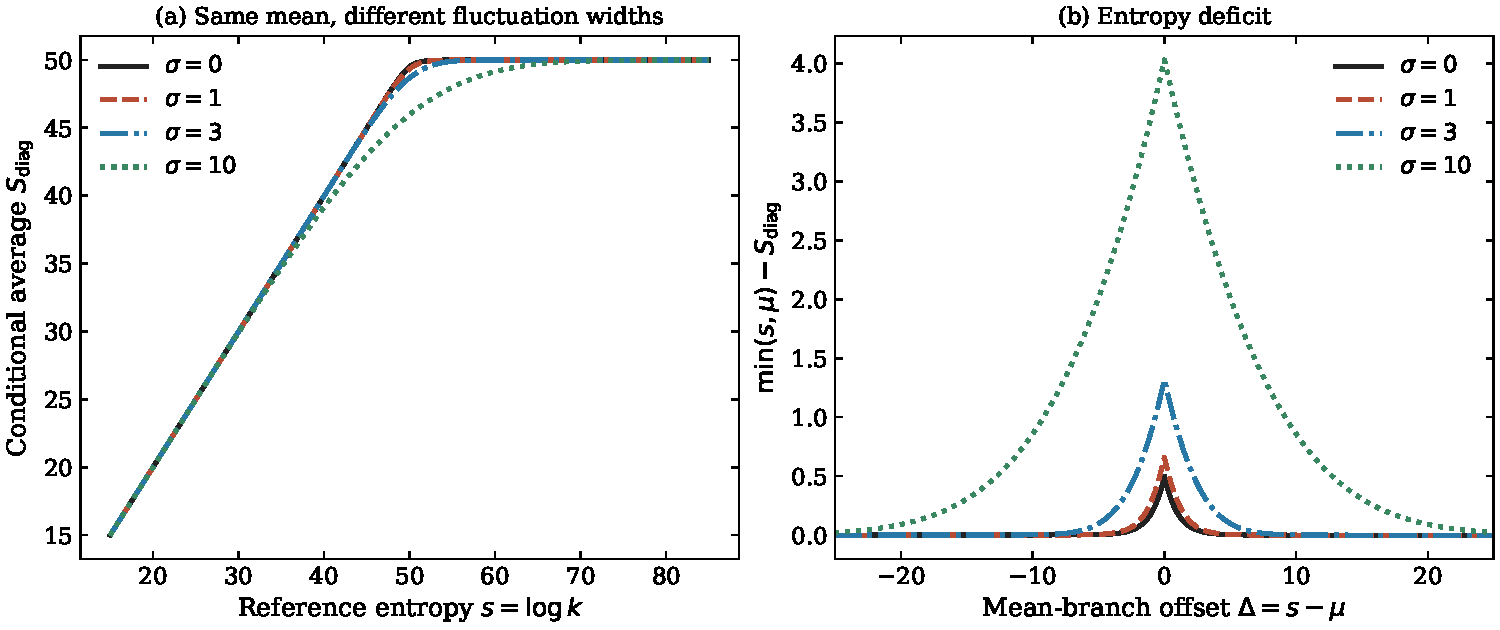
\includegraphics[width=0.9\textwidth]{figures/output/fig08_broadened_page_curve.pdf}
 \caption{Gaussian conditional Page averages defined by
 \eqref{eq08:convolution}, with $\mu=50$ and $\sigma=0,1,3,10$.
 The plotted variable is the reference entropy $s=\log k$.
 All curves use the same mean branch. Increasing the width of its Gaussian
 fluctuation rounds the transition; these curves do not independently
 establish the entropy of a gravitational state. The right panel displays
 the central deficit relative to the minimum of the mean branches.}
 \label{fig08:broadened_page_curve}
\end{figure}

\subsection{An order-one distinction from the planar spectrum}

The full diagonal approximation should not be confused with the planar
entropy in \eqref{eq08:planar_model}, even when both share the same leading
broadening. Set $\delta=K-s$ and $q=\Pr(\delta>0)$. For a family of canonical
laws with $\mathbb E_P a<\infty$, suppose
\begin{equation}
 \Pr(|\delta|\leq A)\longrightarrow0\quad\hbox{for every fixed }A>0,
 \qquad q\longrightarrow q_*\in(0,1).
 \label{eq08:spreading}
\end{equation}
The broad-distribution result of Paper~I \citep{wuebben2026paper1} is
\begin{equation}
 S_{\mathrm{planar}}-S_{\mathrm{diag}}
 \longrightarrow -q_*\log q_*.
 \label{eq08:planar_gap}
\end{equation}
This assertion concerns the specified planar spectral model. It is not a
general theorem about averaging gravitational entropies. At the centered
crossing of a broad symmetric law, $q_*=1/2$, giving $\tfrac12\log2$.
The leading deficit grows with the width, so the relative error decreases,
but the additive error does not vanish.

The spectrum gives a physical explanation. Canonical levels whose individual
probabilities are much smaller than $1/k$ collectively contribute an
approximately uniform spectral component of total weight $q_*$. Its entropy
contains $-q_*\log q_*$ in addition to $q_*\log k$. The diagonal Page average
retains the latter but omits the former. Related spectral components already
appear in the canonical replica analysis of \citet{pssyetal2022}; the
companion result evaluates the limiting difference. The Gaussian correction
in \eqref{eq08:broadened_corr} belongs to the diagonal approximation and does
not supply this missing order-one spectral contribution.

\subsection{A useful identity beyond the Gaussian case}
\label{subsec08:bachelier}

For any real $X$ and fixed threshold $a$,
\begin{equation}
 \min(X,a)=a-(a-X)^+,
 \label{eq08:min_put_identity}
\end{equation}
and hence
\begin{equation}
 \mathbb E\min(X,a)=a-\mathbb E(a-X)^+.
 \label{eq08:min_put_expectation}
\end{equation}
For $X\sim\mathcal N(\mu,\sigma^2)$, the half-line integral is
\begin{equation}
 \mathbb E(a-X)^+=(a-\mu)\Phi((a-\mu)/\sigma)
                  +\sigma\phi((a-\mu)/\sigma).
 \label{eq08:bachelier_put}
\end{equation}
This is also the Gaussian integral in Bachelier's option-pricing formula
\citep{bachelier1900}; no financial interpretation is required here.
For a general centered fluctuation with density $p_\xi$, the same identity
gives $-M''(\Delta)=p_\xi(\Delta)$. Thus the curvature of an averaged minimum
directly records its fluctuation density.

For example, equally likely values $\xi=\pm a$ give a deficit $a/2$ at the
center and two distinct changes of slope, rather than a rounded Gaussian
corner. A quartic density gives another explicit profile. These examples
show why variance alone is insufficient outside a Gaussian regime.
The next section develops the thermodynamic distributions that can supply
such inputs, while keeping the quantum-entropy interpretation separate.

\section{Thermodynamic Ensembles and Critical Fluctuations}
\label{sec09:higher_dimensions}

The Gaussian integral of the preceding section does not depend on spacetime
dimension. Its physical input does: a state preparation, a probability law,
and a fluctuating difference between candidate entropy branches. This section
works through several examples. Neutral AdS black holes provide regular
stable saddles; finite reservoirs impose energy constraints; a charged
critical point replaces the Gaussian law by a quartic one. JT gravity supplies
an explicitly normalized distribution for which the distinction between
geometric entropy and modular energy can be checked directly.

The thermodynamic formulas are standard. The particular finite-size critical
profile and its use in the canonical random-state model follow
Paper~II \citep{wuebben2026paper2}. They should be read with the distinction
between an averaged minimum, the full diagonal Page average, and a planar
spectral entropy established in Section~\ref{sec08:area_fluctuations}.

\subsection{Regular neutral AdS saddles}
\label{subsec09:universal_broadening}

For a Schwarzschild--AdS black hole in bulk dimension $d+1\geq4$,
\begin{align}
 S_*&=\frac{\Omega_{d-1}r_+^{d-1}}{4G},&
 T_H&=\frac{d-2+d r_+^2/\ell^2}{4\pi r_+},\nonumber\\
 C_B&=T_H\frac{dS_*/dr_+}{dT_H/dr_+}
 =(d-1)S_*\frac{d r_+^2/\ell^2+d-2}
                    {d r_+^2/\ell^2-d+2}.
 \label{eq09:neutral_thermodynamics}
\end{align}
Here $\ell$ is the AdS length, $\Omega_{d-1}$ the area of the unit
$(d-1)$-sphere, and the derivative holds $\ell$ fixed. The heat capacity is
positive for $r_+>\ell\sqrt{(d-2)/d}$. To avoid both metastability and phase
coexistence, first take $r_+/\ell>1$ fixed and let $G\to0$. The black-hole
phase then dominates thermal AdS in the usual Hawking--Page comparison
\citep{hawkingpage1983,witten1998}.

If the density-of-states model is $e^{S(E)}\,dE/E_0$, with $E_0$ a fixed
energy unit, the canonical distribution near this saddle is Gaussian at
leading order. For a deterministic competing branch and a fluctuating
thermodynamic entropy, the variance is
\begin{equation}
 \sigma_S^2\simeq C_B.
 \label{eq09:sigma_squared}
\end{equation}
For the canonical modular energy $K=\beta E+\log Z$ the corresponding exact
identity is $\operatorname{Var}K=C_{\mathrm{can}}$, and its leading
semiclassical value is again $C_B$. In either case the Gaussian diagonal
average, with mean $\mu$ and $\Delta=s-\mu$, is
\begin{equation}
 S_{\mathrm{diag}}(s)
 =\int_{\mathbb R}S_{\mathrm{fixed}}(s,\mu+x)
      \frac{e^{-x^2/(2\sigma^2)}}{\sqrt{2\pi\sigma^2}}\,dx.
 \label{eq09:convolution}
\end{equation}
This equation uses the full fixed-dimension kernel defined in
\eqref{eq08:penington_leading}; dropping its exponential term gives the
averaged minimum.

The frequently used large-radius estimate is
\begin{equation}
 \sigma_S\simeq\sqrt{(d-1)S_*},
 \qquad r_+/\ell\gg1.
 \label{eq09:sigma_large_bh}
\end{equation}
There are two independent approximations here. The Gaussian law requires a
well-controlled thermodynamic saddle, while replacing $C_B/S_*$ by $d-1$
requires a large geometric radius:
\begin{equation}
 \frac{C_B}{S_*}
 =(d-1)\left[1+\frac{2(d-2)}{d}\frac{\ell^2}{r_+^2}
       +O(\ell^4/r_+^4)\right].
 \label{eq09:large_radius}
\end{equation}
Increasing $S_*$ by reducing $G$ at fixed radius improves the first
approximation but leaves the geometric correction unchanged.

For a Gaussian law the central deficit of the averaged minimum is
\begin{equation}
 B(0)=\sqrt{\frac{C_B}{2\pi}}
 \simeq\sqrt{\frac{(d-1)S_*}{2\pi}}
 \quad\hbox{at large radius}.
 \label{eq09:peak_deficit}
\end{equation}
It grows in absolute entropy units while decreasing relative to $S_*$. At
$r_+/\ell=2$, the ratios $C_B/S_*$ in bulk dimensions four, five, and six are
$26/11$, $27/7$, and $92/17$, respectively. These differ appreciably from
their large-radius limits $2$, $3$, and $4$. Figure~\ref{fig09:sigma_vs_dimension}
shows both the geometric dependence and the large-radius comparison.
The dimensions are compared at equal $S_*$; this is not a comparison at fixed
mass across different theories.

\begin{figure}[t]
 \centering
 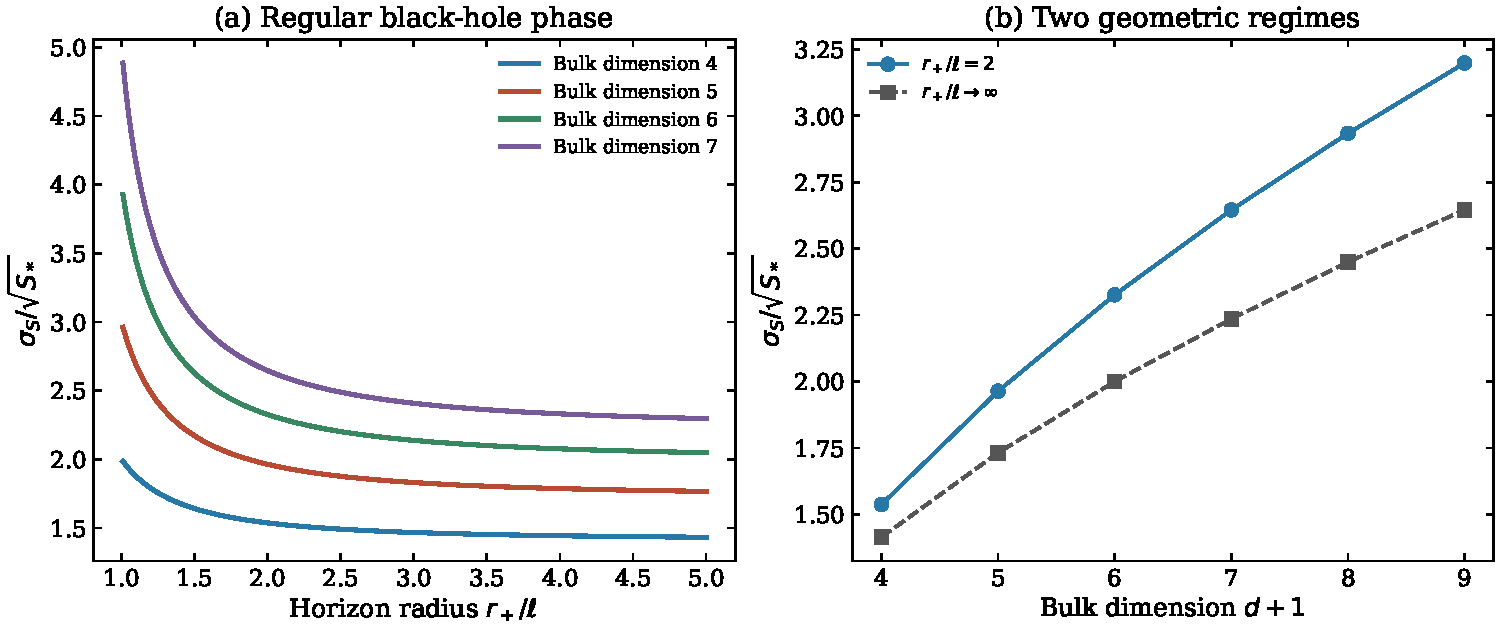
\includegraphics[width=0.94\textwidth]{figures/output/fig09_sigma_vs_dimension.pdf}
 \caption{Leading regular-phase entropy width
 $\sigma_S/\sqrt{S_*}=\sqrt{C_B/S_*}$ for neutral AdS black holes.
 Left: its dependence on $r_+/\ell>1$ in several bulk dimensions.
 Right: values at $r_+/\ell=2$ and the separate large-radius limit, as
 functions of the bulk dimension $d+1$. The curves describe a single stable
 black-hole phase; no extrapolation through a spinodal is made.}
 \label{fig09:sigma_vs_dimension}
\end{figure}

\subsection{Fixed total energy and a finite reservoir}
\label{subsec09:central_distinction}

Fixing the black-hole energy and fixing the total energy of a black hole plus
reservoir impose different constraints. Let
$E_B+E_R=E_{\mathrm{tot}}$ and suppose the two systems can exchange energy.
Their density-of-states distribution is
\begin{equation}
 p(E_B)\,dE_B\propto
 \exp\!\left[S_B(E_B)+S_R(E_{\mathrm{tot}}-E_B)\right]dE_B.
 \label{eq09:finite_bath}
\end{equation}
At a stationary point the temperatures agree. Put
$\epsilon=E_B-E_{B,*}$, and let $C_B$ and $C_R$ be the heat capacities at
the common temperature $T$. The entropy expansion is
\begin{equation}
 S_B+S_R=S_{\mathrm{tot},*}
 -\frac{\epsilon^2}{2T^2}
       \left(\frac1{C_B}+\frac1{C_R}\right)+O(\epsilon^3).
 \label{eq09:bath_hessian}
\end{equation}
If this quadratic maximum controls the distribution, then
\begin{equation}
 \operatorname{Var}E_B\simeq T^2C_{\mathrm{eff}},\qquad
 C_{\mathrm{eff}}=\left(C_B^{-1}+C_R^{-1}\right)^{-1},
 \qquad C_B^{-1}+C_R^{-1}>0.
 \label{eq09:sigma_micro}
\end{equation}
The final inequality is the local stability condition. Positive capacities
make $C_{\mathrm{eff}}$ their harmonic combination. As $C_R/C_B\to\infty$
with $C_B>0$, the canonical result is recovered:
\begin{equation}
 \operatorname{Var}S_B\simeq C_{\mathrm{eff}}\longrightarrow C_B.
 \label{eq09:sigma_canonical}
\end{equation}
For a genuinely small reservoir, its full entropy function may be needed;
a heat capacity at one energy does not guarantee a Gaussian distribution.

The first law also gives
$\delta S_B=\epsilon/T$ and $\delta S_R=-\epsilon/T$ to linear order.
It follows that
\begin{equation}
 \operatorname{Var}S_B\simeq C_{\mathrm{eff}},\qquad
 \operatorname{Var}(S_B-S_R)\simeq4C_{\mathrm{eff}}.
 \label{eq09:bath_gap_variance}
\end{equation}
The second relation, not the first, governs the averaged minimum if the
competing branches are the two subsystem entropies. Energy conservation makes
their fluctuations anticorrelated. Treating one branch as fixed would miss a
factor of two in the standard deviation.

A numerical example makes the distinction explicit. Take two regular systems
with $C_B=C_R=100$, at equal mean entropies. Then $C_{\mathrm{eff}}=50$.
The entropy standard deviation of either system is $\sqrt{50}$, whereas
the standard deviation of their difference is $\sqrt{200}$. The leading
central deficit of their averaged minimum is
\begin{equation}
 B(0)=\frac{\sqrt{200}}{\sqrt{2\pi}}
     =\frac{10}{\sqrt{\pi}}\simeq5.641896.
 \label{eq09:bath_example}
\end{equation}
It is compatible with an exactly fixed total energy. This is the same
thermodynamic mechanism that gives an enhanced correction for an equal
bipartition in the energy-eigenstate analysis of
\citet{murthysrednicki2019}.

\begin{table}[t]
 \centering
 \caption{Distinct constraints in a regular quadratic regime.
 Each variance concerns the indicated observable. An actual entanglement
 calculation must also specify the sector structure of the state.}
 \label{tab09:micro_vs_canonical}
 \begin{adjustbox}{max width=\textwidth}
 \begin{tabular}{lll}
 \toprule
 Preparation & Fluctuating quantity & Leading variance\\
 \midrule
 Fixed $E_B$ & $S_B(E_B)$ & $0$ from energy exchange\\
 Infinite reservoir, $C_B>0$ & $S_B$ & $C_B$\\
 Fixed $E_B+E_R$, stable finite bath & $S_B$ & $C_{\mathrm{eff}}$\\
 Same finite bath, two entropy branches & $S_B-S_R$ & $4C_{\mathrm{eff}}$\\
 \bottomrule
 \end{tabular}
 \end{adjustbox}
\end{table}

The total entropy $S_B+S_R$, by contrast, is stationary at equilibrium.
Its fluctuation starts quadratically and is order one in the Gaussian
approximation. It must not be substituted for the fluctuating branch
difference. More generally, if that difference is $g(E_B)$ under the energy
constraint, its leading variance is $g'(E_{B,*})^2\operatorname{Var}E_B$.
A common mode can cancel, and a vanishing linear derivative requires a new
expansion.

These equilibrium statements do not determine the time-dependent state of
an evaporating black hole. To apply them dynamically, one needs a preparation
and an approximation justifying the instantaneous distribution, together
with the relevant entropy branches. Unitarity or fixed total energy alone
does not select a sharp or broad Page transition.

\subsection{Negative heat capacity}
\label{subsec09:negative_cv}

For an asymptotically flat Schwarzschild black hole in bulk dimension
$d+1\geq4$,
\begin{equation}
 C_B=-(d-1)S_B<0.
 \label{eq09:cv_flat}
\end{equation}
Indeed $T_H\propto r_+^{-1}$ while $S_B\propto r_+^{d-1}$.
Such a branch is unstable in contact with an infinite reservoir of fixed
temperature: increasing its energy lowers its temperature, encouraging
further inflow. The unrestricted asymptotically flat canonical integral also
fails because the black-hole density of states grows too rapidly.

The finite-reservoir stability condition in \eqref{eq09:sigma_micro} is
different. A positive reservoir with $C_R<|C_B|$ can make the combined entropy
locally concave along the allowed energy exchange. For example,
$C_B=-100$ and $C_R=25$ give $C_{\mathrm{eff}}=100/3>0$.
This is a local thermodynamic statement; it does not prove global stability
or construct a gravitational equilibrium boundary condition. Cavity
thermodynamics illustrates why boundary conditions matter
\citep{york1986}. Negative heat capacity therefore rules out an unrestricted
canonical treatment of that branch, but does not force every allowed
fixed-total-energy state to have negligible subsystem fluctuations.

\subsection{Spinodal, coexistence, and continuous criticality}
\label{subsec09:critical_phenomena}

Three distinct phenomena are often placed under the heading of a
thermodynamic transition. They require different probability laws.

\paragraph{The neutral AdS spinodal.}
The minimum temperature of the neutral black-hole family occurs at
\begin{equation}
 r_0=\ell\sqrt{\frac{d-2}{d}},\qquad
 T_0=\frac{\sqrt{d(d-2)}}{2\pi\ell}.
 \label{eq09:spinodal_location}
\end{equation}
Set $N_0=S(r_0)$, $x=r_+/r_0-1$, and $t_0=(T-T_0)/T_0$.
The action $I=M/T-S$ has the local form
\begin{equation}
 I(x)-I(0)
 =(d-1)N_0\left(\frac{x^3}{6}-t_0x\right)
 +O\!\left(N_0[x^4+|t_0|x^2+t_0^2|x|]\right).
 \label{eq09:spinodal_action}
\end{equation}
For $t_0>0$, the stable and unstable stationary radii lie near
$x_\pm=\pm\sqrt{2t_0}$. The stable saddle's response obeys
\begin{equation}
 C_B\sim(d-1)N_0(2t_0)^{-1/2},
 \label{eq09:cv_hp}
\end{equation}
and its Gaussian entropy width is
\begin{equation}
 \sigma_S\sim\sqrt{(d-1)N_0}\,(2t_0)^{-1/4}.
 \label{eq09:sigma_hp}
\end{equation}
The barrier is of order $N_0t_0^{3/2}$. A well-localized Gaussian therefore
requires $t_0\gg N_0^{-2/3}$. The apparent divergence cannot be extrapolated
past that condition. The cubic local action is not confining on the real
line, so it does not define a replacement equilibrium distribution by itself.
A distribution conditioned to remain in a metastable basin needs an explicit
basin prescription or dynamical construction.

\paragraph{Hawking--Page coexistence.}
The Hawking--Page temperature is instead
$T_{\mathrm{HP}}=(d-1)/(2\pi\ell)$, at $r_+=\ell$.
It exceeds $T_0$ \citep{hawkingpage1983}. The black-hole branch there has
finite heat capacity $C_B=(d-1)^2S_{\mathrm{HP}}$. Between $T_0$ and
$T_{\mathrm{HP}}$ it is metastable relative to thermal AdS, even when its
local heat capacity is positive.

When both phases are retained, the choice of phase supplies another
fluctuation. If their probabilities are $w$ and $1-w$, with conditional means
$\mu_B,\mu_A$ and variances $V_B,V_A$ of a chosen observable, then
\begin{equation}
 V=wV_B+(1-w)V_A+w(1-w)(\mu_B-\mu_A)^2.
 \label{eq09:coexistence_variance}
\end{equation}
For modular energy at coexistence, the mean separation is extensive.
A mixture with both weights of order one can therefore have width of order
the entropy, even though each phase has an ordinary square-root width.
It is bimodal. Replacing it by a Gaussian of the same variance loses its
two changes of slope in the averaged minimum. For two equally weighted
narrow components separated by $D$, the central deficit is $D/4$.
The coexistence window has relative temperature width of order
$S_{\mathrm{HP}}^{-1}$, with finite-size shifts depending on phase prefactors.

\paragraph{The charged continuous critical point.}
For a spherical RN--AdS black hole, choose the charge parameter $q$ so that
\begin{equation}
 T_H(r)=\frac{1}{4\pi r}
 \left(d-2+\frac{dr^2}{\ell^2}
       -\frac{(d-2)q^2}{r^{2d-4}}\right),
 \qquad S(r)=\frac{\Omega_{d-1}r^{d-1}}{4G}.
 \label{eq09:rn_temperature}
\end{equation}
The fixed-charge small--large black-hole transition has a critical endpoint
\citep{chamblin1999,kubiznakmann2012}. At that endpoint,
\begin{equation}
 r_c^2=\frac{(d-2)^2\ell^2}{d(d-1)},\qquad
 q_c^2=\frac{r_c^{2d-4}}{(2d-3)(d-1)},\qquad
 T_c=\frac{(d-2)^2}{\pi(2d-3)r_c}.
 \label{eq09:critical_geometry}
\end{equation}
Here $T_H'(r_c)=T_H''(r_c)=0$. Let $N=S(r_c)$, $R=r/r_c$, and hold the
critical geometry fixed while $G\to0$, so $N\to\infty$. In the density-of-states
model $e^{S(E)}dE/E_0$ on the physical RN outer-horizon family, the first law
gives
\begin{equation}
 \frac{dI_c}{dR}
 =N(d-1)R^{d-2}\left(\frac{T_H(R)}{T_c}-1\right),
 \qquad I_c=\beta_c M-S.
\end{equation}
Since $T_H/T_c-1=(2d-3)(R-1)^3/6+\cdots$,
\begin{equation}
 I_c(R)-I_c(1)=Na_d(R-1)^4+O(N(R-1)^5),
 \qquad a_d=\frac{(d-1)(2d-3)}{24}.
 \label{eq09:quartic_action}
\end{equation}
The first restoring term is quartic and positive. Within this RN family
the critical saddle is the global minimum; applying the construction to a
larger theory requires checking additional phases and instabilities.

Put
\begin{equation}
 X=(a_dN)^{1/4}(R-1),\qquad
 L_N=(d-1)a_d^{-1/4}N^{3/4}.
 \label{eq09:critical_scales}
\end{equation}
The energy measure contains the Jacobian $M'(R)dR$, smooth and positive at
$R=1$. It is constant to leading order on this shrinking neighborhood.
The resulting normalized limiting density is
\begin{equation}
 p_0(X)=\frac{2}{\Gamma(1/4)}e^{-X^4}.
 \label{eq09:quartic_density}
\end{equation}
The centered $S$ and $K$ divided by $L_N$ both tend to $X$ in this model.
Their common leading entropy standard deviation and central averaged-minimum
deficit are
\begin{equation}
 \sigma\sim L_N
 \sqrt{\frac{\Gamma(3/4)}{\Gamma(1/4)}},\qquad
 B(0)\sim\frac{L_N\sqrt{\pi}}{2\Gamma(1/4)}.
 \label{eq09:quartic_observables}
\end{equation}
For example,
$\int_0^\infty x^m e^{-x^4}dx=\tfrac14\Gamma((m+1)/4)$ immediately gives
both moments. Their ratio is $B(0)/\sigma=2^{-5/4}$, distinct from the
Gaussian value $1/\sqrt{2\pi}$. The width is finite at every finite $N$,
grows as $N^{3/4}$, and decreases relative to the extensive entropy as
$N^{-1/4}$. In the canonical random-state model, the broad-distribution
planar correction from \eqref{eq08:planar_gap} remains order one.

\subsection{The finite-temperature critical crossover}

Let $t=(T-T_c)/T_c$ at $q=q_c$. The exact action relation
\begin{equation}
 I_\beta(R)-I_\beta(1)
 =\frac{I_c(R)-I_c(1)-t[S(R)-N]}{1+t}
\end{equation}
shows that the correct thermal scaling variable is $h=L_Nt$.
At fixed $h$, the limiting density becomes
\begin{equation}
 p_h(X)=\frac{e^{-X^4+hX}}{\mathcal Z(h)},\qquad
 \mathcal Z(h)=\int_{\mathbb R}e^{-x^4+hx}\,dx.
 \label{eq09:thermal_quartic}
\end{equation}
Write $\mu_h=\mathbb E_hX$ and $v_h=\operatorname{Var}_hX$. The centered
entropy profile at $\Delta=zL_N$ is
\begin{equation}
 \frac{B(zL_N)}{L_N}\longrightarrow
 \frac12\left[\mathbb E_h|z-X+\mu_h|-|z|\right],
 \qquad \frac{\sigma}{L_N}\longrightarrow\sqrt{v_h}.
 \label{eq09:critical_profile}
\end{equation}
The averaged entropy is smooth through this finite crossover for
$|t|=O(N^{-3/4})$. Its deficit relative to the sharp minimum contains
a cusp at $z=0$ because the reference minimum itself has a cusp.

For large $|h|$, the maximum of the density is near
$X_*=(h/4)^{1/3}$, with Gaussian variance $(12X_*^2)^{-1}$.
Equivalently, writing $b_d=(2d-3)/6$, the regular saddle outside the critical
window obeys
\begin{equation}
 C_B\sim\frac{(d-1)N}{3b_d^{1/3}}|t|^{-2/3},
 \qquad N^{-3/4}\ll|t|\ll1,
 \label{eq09:cv_vdw}
\end{equation}
and hence
\begin{equation}
 \sigma\sim
 \sqrt{\frac{d-1}{3b_d^{1/3}}}\,N^{1/2}|t|^{-1/3}.
 \label{eq09:sigma_vdw}
\end{equation}
The familiar critical response exponent describes this outer Gaussian
regime. The quartic law supplies its finite-size continuation, rather than
an unlimited width at $t=0$.

\begin{figure}[t]
 \centering
 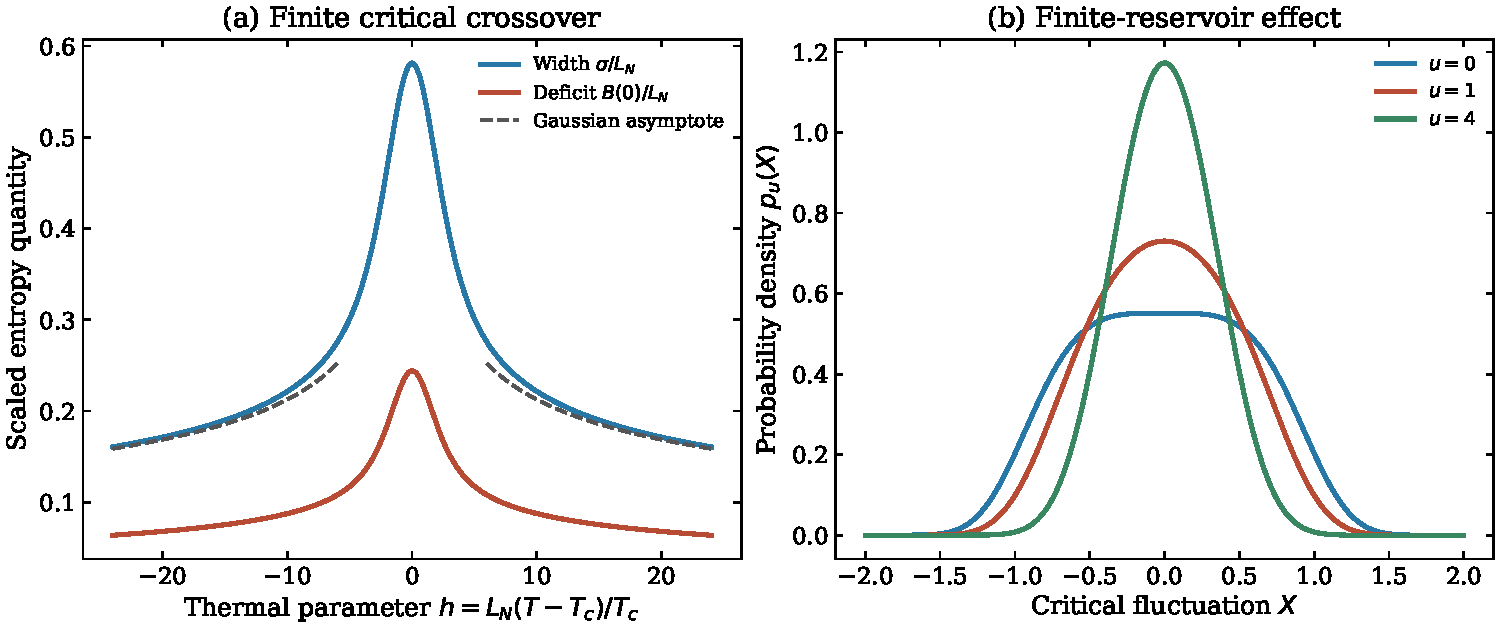
\includegraphics[width=0.96\textwidth]{figures/output/fig09_critical_divergence.pdf}
 \caption{Controlled critical crossover from the normalized density
 $p_h(X)\propto e^{-X^4+hX}$. Left: the finite width $\sigma/L_N$ and
 central deficit $B(0)/L_N$; the dashed curve is the Gaussian large-$|h|$
 width, displayed only away from $h=0$. Right: the critical density modified
 by a reservoir, $p_u(X)\propto e^{-X^4-uX^2}$, for several $u$.
 These are limiting distributions of the specified thermodynamic model,
 not extrapolations of a divergent Gaussian variance.}
 \label{fig09:critical_divergence}
\end{figure}

\subsection{How large must a critical reservoir be?}

At the critical point, expand a reservoir entropy around equilibrium:
\begin{equation}
 S_R(E_{R,c}-\epsilon)
 =S_R(E_{R,c})-\frac{\epsilon}{T_c}
  -\frac{\epsilon^2}{2T_c^2C_R}+\mathcal R_R(\epsilon).
 \label{eq09:critical_reservoir}
\end{equation}
On the canonical critical scale,
$\epsilon/T_c=L_NX+o(L_N)$. If the remainder tends to zero on bounded
$X$ intervals, the allowed energy domain includes these intervals, and the
composite distribution has sufficiently controlled tails to pass to its
first two moments, the combined law is
\begin{equation}
 p_u(X)=\frac{e^{-X^4-uX^2}}{Z_u},\qquad
 u=\lim_{N\to\infty}\frac{L_N^2}{2C_R}\geq0.
 \label{eq09:reservoir_quartic}
\end{equation}
The tail requirement is separate from a Taylor expansion: rare distant
energies must not carry a finite share of the scaled variance.

The canonical quartic limit requires $u=0$, or $C_R\gg N^{3/2}$.
A reservoir with $C_R\asymp N^{3/2}$ changes the shape at leading order.
In the reservoir-limited regime $C_R\to\infty$ but $C_R\ll N^{3/2}$,
the appropriate scale becomes $\sqrt{C_R}$. Provided the same local and
tail control hold on that narrower scale, the law becomes Gaussian and
$\sigma_B\sim\sqrt{C_R}$. An ordinary extensive reservoir, with capacity
of order $N$, is therefore insufficient to reproduce the canonical
critical width. If the two competing branches are $S_B$ and $S_R$, their
leading difference is $2L_NX$, so both its width and central deficit are
twice the one-fluctuating-branch values.

This is a concrete consequence of the state preparation. It also supplies
a useful test for applications: identify the thermodynamic mode, determine
the constraint, and compute its coupling to the branch difference before
assigning a critical exponent to an entropy transition.

\subsection{A normalized JT example}
\label{subsec09:jt_corrections}

For the disk Schwarzian density, in units with Schwarzian coupling one,
\begin{equation}
 \rho_0(E)=\frac{e^{S_0}}{2\pi^2}
       \sinh(2\pi\sqrt{2E}),\qquad E\geq0.
 \label{eq09:schwarzian_energy}
\end{equation}
This is the density per unit $dE$ \citep{saadetal2019}. It is the disk
density, not a nonperturbative completion of JT gravity. Its canonical
probability is proportional to $\rho_0(E)e^{-\beta E}dE$.
Define the geometric entropy shift $x=S_{\mathrm{BH}}-S_0=2\pi\sqrt{2E}$.
Since $dE=x\,dx/(4\pi^2)$, its normalized density is
\begin{align}
 p_\beta(x)&=\frac{x\sinh x\,e^{-\beta x^2/(8\pi^2)}}{Z_x(\beta)},
 \qquad x\geq0,\nonumber\\
 Z_x(\beta)&=\int_0^\infty x\sinh x\,e^{-\beta x^2/(8\pi^2)}dx.
 \label{eq09:jt_entropy_density}
\end{align}
The factor $x$ is the Jacobian. Omitting it changes the mean, variance, and
the resulting conditional entropy average.

The disk partition function is proportional to
$e^{S_0}\beta^{-3/2}e^{2\pi^2/\beta}$. Therefore
\begin{equation}
 \langle E\rangle=\frac{2\pi^2}{\beta^2}+\frac{3}{2\beta},
 \qquad C_{\mathrm{can}}=\frac{4\pi^2}{\beta}+\frac32
                      =\operatorname{Var}K.
 \label{eq09:jt_modular_variance}
\end{equation}
These identities are exact within the disk density. They are not formulas
for $\operatorname{Var}x$. For the latter, the distribution
\eqref{eq09:jt_entropy_density} can be integrated directly. Define its
skewness by
\begin{equation}
 \gamma_1=\frac{\mathbb E(x-\langle x\rangle)^3}
               {(\operatorname{Var}x)^{3/2}}.
 \label{eq09:skewness}
\end{equation}
The values in Table~\ref{tab09:jt_moments} come from the saved quadrature
calculation accompanying this section. Neither the centered geometric
distribution nor the centered modular distribution depends on $S_0$;
the extremal degeneracy shifts entropy means.

\begin{table}[t]
 \centering
 \caption{Moments of the geometric entropy shift $x$ from the normalized
 disk JT density \eqref{eq09:jt_entropy_density}. The final column is the
 distinct canonical modular-energy variance.}
 \label{tab09:jt_moments}
 \begin{adjustbox}{max width=\textwidth}
 \begin{tabular}{ccccc}
 \toprule
 $\beta/\pi$ & $\langle x\rangle$ & $\operatorname{sd}(x)$
 & $\gamma_1$ & $\operatorname{Var}K$\\
 \midrule
 $1$ & $13.566324$ & $3.401121$ & $0.050218$ & $14.066371$\\
 $2$ & $7.280839$  & $2.305939$ & $0.134644$ & $7.783185$\\
 $4$ & $4.119496$  & $1.524513$ & $0.262853$ & $4.641593$\\
 \bottomrule
 \end{tabular}
 \end{adjustbox}
\end{table}

Figure~\ref{fig09:three_layer_comparison} isolates the effect of this
non-Gaussian shape on a defined conditional average. It compares a
fixed kernel at the mean geometric entropy, its average against a Gaussian
with the same mean and variance, and its average against the full density
\eqref{eq09:jt_entropy_density}. Matching the variance avoids attributing a
width error to skewness. All three curves use the same conditional Page
kernel. None is labeled the exact planar JT entropy.

\begin{figure}[t]
 \centering
 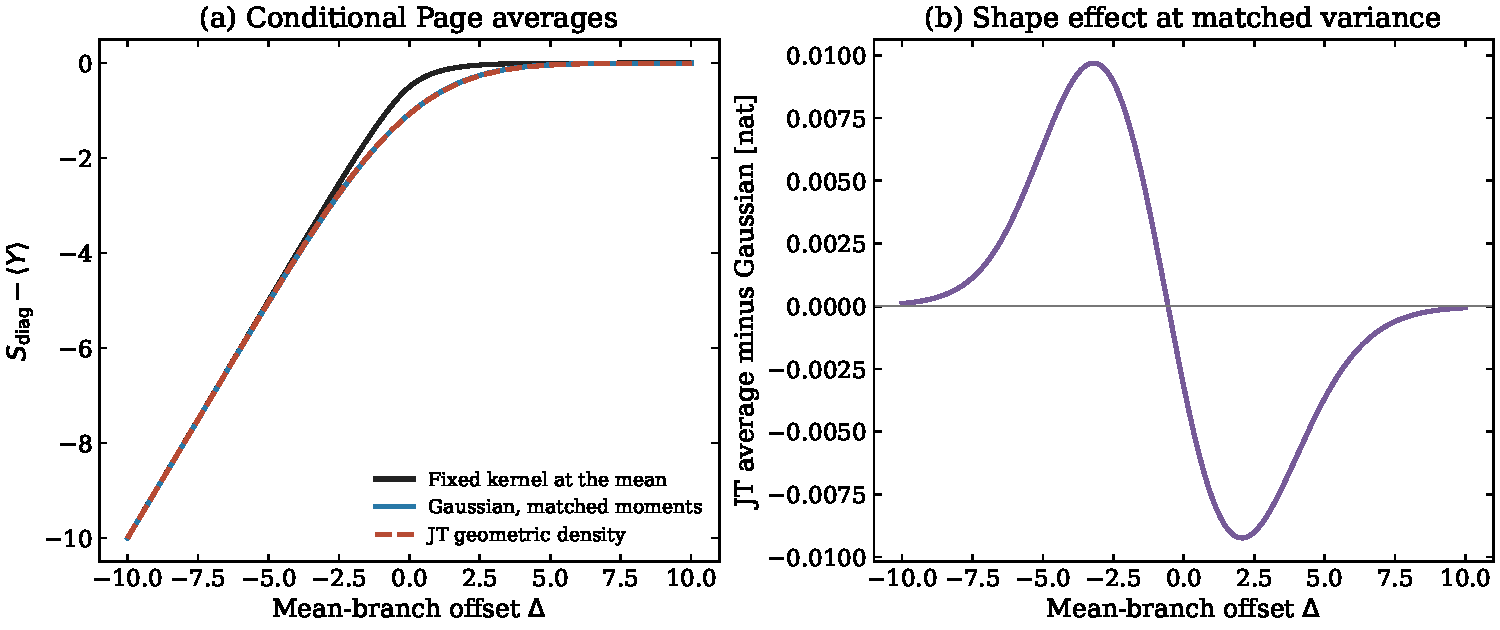
\includegraphics[width=0.94\textwidth]{figures/output/fig09_three_layer_comparison.pdf}
 \caption{Conditional Page averages for the geometric entropy
 $Y=S_0+x$, at $\beta=2\pi$ and $S_0=20$.
 Left: the fixed kernel, a Gaussian average with matched moments, and
 numerical integration against the normalized JT density.
 Right: the difference between the two averages, isolating distribution
 shape at the same variance.
 The JT standard deviation is $2.305939$ and skewness is $0.134644$.
 These are diagonal conditional averages using $Y=S_{\mathrm{BH}}$;
 the canonical random-state calculation instead uses $Y=K$ and its planar
 spectrum is a separate calculation.}
 \label{fig09:three_layer_comparison}
\end{figure}

At high temperature the action has a well-separated saddle, and the leading
geometric width $\sqrt{4\pi^2/\beta}$ captures the dominant scale.
At moderate temperature the lower boundary and non-Gaussian shape matter.
For the canonical random-state model, one should push the same energy law
forward to $K=\beta E+\log Z$ and then compute its diagonal or planar entropy
as appropriate. Improving the probability distribution in a conditional
average is distinct from replacing that average by a spectral calculation.
It is also distinct from adding higher gravitational topologies.

\subsection{What these examples establish}
\label{subsec09:summary}

The regular Gaussian profile follows from a quadratic saddle and a specified
fluctuating branch difference. Its width often scales as the square root of
an extensive heat capacity, with coefficients depending on geometry and
constraints. A finite total energy still permits fluctuations of subsystems,
and their anticorrelation changes the relevant entropy difference.

At a charged continuous critical point the quartic action gives a finite
$N^{3/4}$ width in the canonical model, a thermal window of order $N^{-3/4}$,
and a reservoir crossover at capacity of order $N^{3/2}$. A spinodal instead
marks the failure of a metastable saddle, while coexistence produces a
mixture of distinct phases. These distributions should be treated separately.

Finally, thermodynamic entropy, canonical modular energy, averaged
conditional entropy, and planar spectral entropy are distinct quantities.
Their leading broad limits can agree without their order-one corrections
agreeing. Keeping those distinctions explicit allows the subsequent discussion
of higher moments and replica topology to address identifiable observables.

\section{Genus Corrections and the Topological Expansion}
\label{sec10:genus_corrections}

The Marchenko--Pastur density is a leading large-dimension result.  To go
beyond it, one must specify both the ensemble and the normalization of the
observable.  This section develops the first correction in the complex
Gaussian/Haar benchmark and then compares its organization with the
continuum JT topology expansion.  Three operations will be kept distinct:
counting nonplanar Wick contractions, normalizing a random state, and adding
handles to a gravitational surface.  All can affect a replica calculation,
but their coefficients are not interchangeable.

\subsection{The genus-one permutation count}
\label{subsec10:genus_one}

\subsubsection{The closed-form formula}
For $c_n=(1\,2\cdots n)$, recall the genus of a contraction,
\begin{equation}
 g(\sigma)=\frac{n+1-C(\sigma)-C(c_n^{-1}\sigma)}2.
 \label{eq10:genus_formula}
\end{equation}
The associated connected ribbon graph has one face, $n$ edges, and
$C(\sigma)+C(c_n^{-1}\sigma)$ vertices, so this equation is Euler's formula.
Genus zero selects the $C_n$ non-crossing permutations.  Genus one requires
\begin{equation}
 C(\sigma)+C(c_n^{-1}\sigma)=n-1.
 \label{eq10:genus_one_condition}
\end{equation}
Let $g_j(n)$ denote the number of permutations of genus $j$.  The classical
genus-one count is
\begin{equation}
 \boxed{g_1(n)=\binom{2n-2}{n-1}\frac{(n-1)(n-2)}{12}.}
 \label{eq10:genus_one_count}
\end{equation}
This is a count of factorizations of a long cycle, or equivalently rooted
bicolored one-face maps; see~\citet{goupilschaeffer1998,corihetyei2014}.
The Harer--Zagier polygon-gluing problem~\citep{harerzagier1986} is related
but counts a different family, so its coefficients should not be substituted
for Eq.~\eqref{eq10:genus_one_count}.  The count is not a new gravitational
result.

One convenient way to extract these numbers is their generating function
\begin{equation}
 \sum_{n\geq3}g_1(n)z^n=\frac{z^3}{(1-4z)^{5/2}}.
 \label{eq10:genus_one_generating}
\end{equation}
Indeed, the binomial series gives the coefficient
$4^{n-3}(5/2)_{n-3}/(n-3)!$, which simplifies to
Eq.~\eqref{eq10:genus_one_count}.  Here the generating-function identity
encodes the combinatorial enumeration; the subsequent coefficient extraction
is elementary.

\subsubsection{Small replica indices and direct enumeration}
The first values are
\begin{equation}
 g_1(1),\ldots,g_1(8)=0,0,1,10,70,420,2310,12012.
 \label{eq10:genus_one_sequence}
\end{equation}
For example, at $n=3$ five permutations are non-crossing and the remaining
permutation $(1\,3\,2)=c_3^{-1}$ has genus one.  At $n=5$, the full
partition of $5!=120$ permutations is $42+70+8$ at genera zero, one, and two.
The accompanying computation enumerates all permutations through $n=8$ and
checks both Euler's formula and the closed form.

\begin{table}[htbp]
\centering
\caption{Permutation counts and their ratios.  A zero in the genus-one
column concerns the Wick numerator; it does not imply that the normalized
moment has no relative correction of order $L^{-2}$.}
\label{tab10:genus_one_values}
\begin{adjustbox}{max width=\textwidth,center}
\begin{tabular}{c r r r r}
\hline
$n$ & $C_n$ & $g_1(n)$ & $g_1(n)/C_n$ & $n^3/48$\\
\hline
1&1&0&0&0.021\\
2&2&0&0&0.167\\
3&5&1&0.200&0.563\\
4&14&10&0.714&1.333\\
5&42&70&1.667&2.604\\
6&132&420&3.182&4.500\\
7&429&2310&5.385&7.146\\
8&1430&12012&8.400&10.667\\
\hline
\end{tabular}
\end{adjustbox}
\end{table}

Dividing the two closed forms gives
\begin{equation}
 \frac{g_1(n)}{C_n}
 =\frac{n(n-1)(n-2)(n+1)}{24(2n-1)}
 \sim\frac{n^3}{48}.
 \label{eq10:genus_ratio}
\end{equation}
Thus genus-one permutations first outnumber planar permutations at $n=5$.
Their numerical count is not their contribution to a moment: the dimension
weights must still be included.

\subsection{Normalized moments beyond the planar limit}
\label{subsec10:higher_genus}

\subsubsection{Balanced dimensions}
Set $k=L$, with $L$ an integer dimension, and use the normalized state of
Eq.~\eqref{eq06:normalizations}.  The exact finite formula becomes
\begin{equation}
 \mathbb E_{\mathrm H}\operatorname{Tr}\rho^n
 =L^{1-n}\frac{L^{2n}}{(L^2)_n}
 \sum_{g=0}^{\lfloor(n-1)/2\rfloor}g_g(n)L^{-2g}.
 \label{eq10:moment_genus_expansion}
\end{equation}
The bound on $g$ follows because each of the two cycle counts is at least
one.  The numerator is a finite polynomial for each integer $n$.
The corresponding mean-normalized moment has the same expression without
$L^{2n}/(L^2)_n$.  In particular its genus-one contribution is exactly
\begin{equation}
 \delta_1\!\left[\mathbb E\operatorname{Tr}\widetilde\rho^n\right]
 =L^{1-n}g_1(n)L^{-2}.
 \label{eq10:genus_one_contribution}
\end{equation}
The normalization factor has its own expansion,
\begin{equation}
 \frac{L^{2n}}{(L^2)_n}
 =\prod_{j=0}^{n-1}\left(1+\frac{j}{L^2}\right)^{-1}
 =1-\frac{n(n-1)}{2L^2}+O(L^{-4}),
 \label{eq10:normalization_expansion}
\end{equation}
for fixed $n$.  Multiplying the numerator and denominator expansions gives
\begin{equation}
 L^{n-1}\mathbb E_{\mathrm H}\operatorname{Tr}\rho^n
 =C_n+\frac{g_1(n)-\tfrac12n(n-1)C_n}{L^2}
 +O(L^{-4}).
 \label{eq10:normalized_first_correction}
\end{equation}
Both terms in the correction are required.  The negative normalization term
can exceed the positive contribution from nonplanar contractions.

\subsubsection{Why purity still has a correction}
\label{subsubsec10:vanishing}
At $n=1$, the exact moment is one.  At $n=2$, $g_1(2)=0$, but the
normalization factor is $L^2/(L^2+1)$.  Hence
\begin{equation}
 \mathbb E_{\mathrm H}\operatorname{Tr}\rho^2
 =\frac{2L}{L^2+1}
 =\frac2L-\frac2{L^3}+O(L^{-5}).
 \label{eq10:purity_correction}
\end{equation}
The leading relative correction is $-L^{-2}$.  This provides a direct
counterexample to identifying absence of a genus-one contraction with absence
of a correction at that order.  For $n=3$ the exact formula is
\begin{equation}
 \mathbb E_{\mathrm H}\operatorname{Tr}\rho^3
 =\frac{5L^2+1}{(L^2+1)(L^2+2)}
 =\frac5{L^2}-\frac{14}{L^4}+O(L^{-6}).
 \label{eq10:third_moment}
\end{equation}
The numerator coefficient $g_1(3)=1$ and the denominator coefficient
$-3C_3=-15$ combine to give $-14$.

For clarity, the resulting order statements are
\begin{equation}
 \frac{\delta\mathbb E\operatorname{Tr}\rho^2}
 {2/L}=O(L^{-2}),\qquad
 \frac{\delta\mathbb E\operatorname{Tr}\rho^3}
 {5/L^2}=O(L^{-2}).
 \label{eq10:sensitivity_ordering}
\end{equation}
They refer to ensemble mean moments.  The average of a R\'enyi entropy is
not obtained by taking the logarithm of its mean moment; the distinction is
examined in Section~\ref{sec12:annealed_quenched}.

\subsubsection{An independent entropy check}
The von Neumann entropy involves a derivative at replica index one, not the
value of one integer moment.  A closed form for $g_1(n)$ at integer $n$ does
not by itself justify differentiating a chosen interpolation of it.  In the
Haar model the exact Page formula~\eqref{eq07:finite_page} provides an
independent calculation:
\begin{equation}
 \mathbb E_{\mathrm H}S(\rho)
 =H_{L^2}-H_L-\frac{L-1}{2L}
 =\log L-\frac12+\frac{7}{12L^2}+O(L^{-4}).
 \label{eq10:entropy_correction}
\end{equation}
Thus the entropy does receive a correction at the same dimension order.
At $L=2$ the exact result is $1/3$ nat, while the leading expression is
$\log2-1/2$.  Equations~\eqref{eq10:purity_correction} and
\eqref{eq10:entropy_correction} check different observables, with different
coefficients, in the same normalized ensemble.

\subsubsection{Unequal dimensions}
At fixed $\gamma=k/L$, the genus-$g$ coefficient is a polynomial in
$\gamma$ rather than the unweighted count $g_g(n)$.  For example, the
mean-normalized expansion is
\begin{equation}
 \mathbb E\operatorname{Tr}\widetilde\rho^n
 =k^{1-n}\sum_g k^{-2g}
 \sum_{\substack{\sigma\in S_n\\g(\sigma)=g}}
 \gamma^{n-C(\sigma)}.
 \label{eq10:unequal_dimensions}
\end{equation}
The normalized answer multiplies this by $(kL)^n/(kL)_n$.
Counting permutations without their cycle numbers is sufficient only at
$\gamma=1$.  More general matrix ensembles change the contraction weights
or even the available contractions, so their finite-size corrections require
an independent calculation.

\subsection{The range of the genus expansion}
\label{subsubsec10:asymptotic}

For fixed $n$ the permutation numerator is finite, whereas its normalized
rational expression has an infinite expansion in inverse dimension.  Neither
fact implies uniform control as $n$ grows with $L$.  At balanced dimensions,
the ratio of the genus-one to planar contribution to the mean-normalized
moment is
\begin{equation}
 \frac{g_1(n)}{C_n L^2}\sim\frac{n^3}{48L^2}.
 \label{eq10:nonuniform_parameter}
\end{equation}
A necessary check for retaining only genus zero is therefore
$n^3/L^2\ll1$.  At $n$ of order $L^{2/3}$, the first omitted term alone is
no longer parametrically small.  This estimate does not establish a complete
uniform asymptotic expansion; it identifies a scale at which a fixed-replica
argument cannot simply be extrapolated.

\begin{remark}[The Catalan/genus-one crossover]
\label{rem10:crossover}
At a fixed small replica index, large dimension suppresses genus one even
when $g_1(n)>C_n$.  If the replica index is allowed to grow, the combinatorial
factor competes with the suppression.  Both the index and dimension must be
specified when claiming that a correction is small.
\end{remark}

\begin{figure}[htbp]
\centering
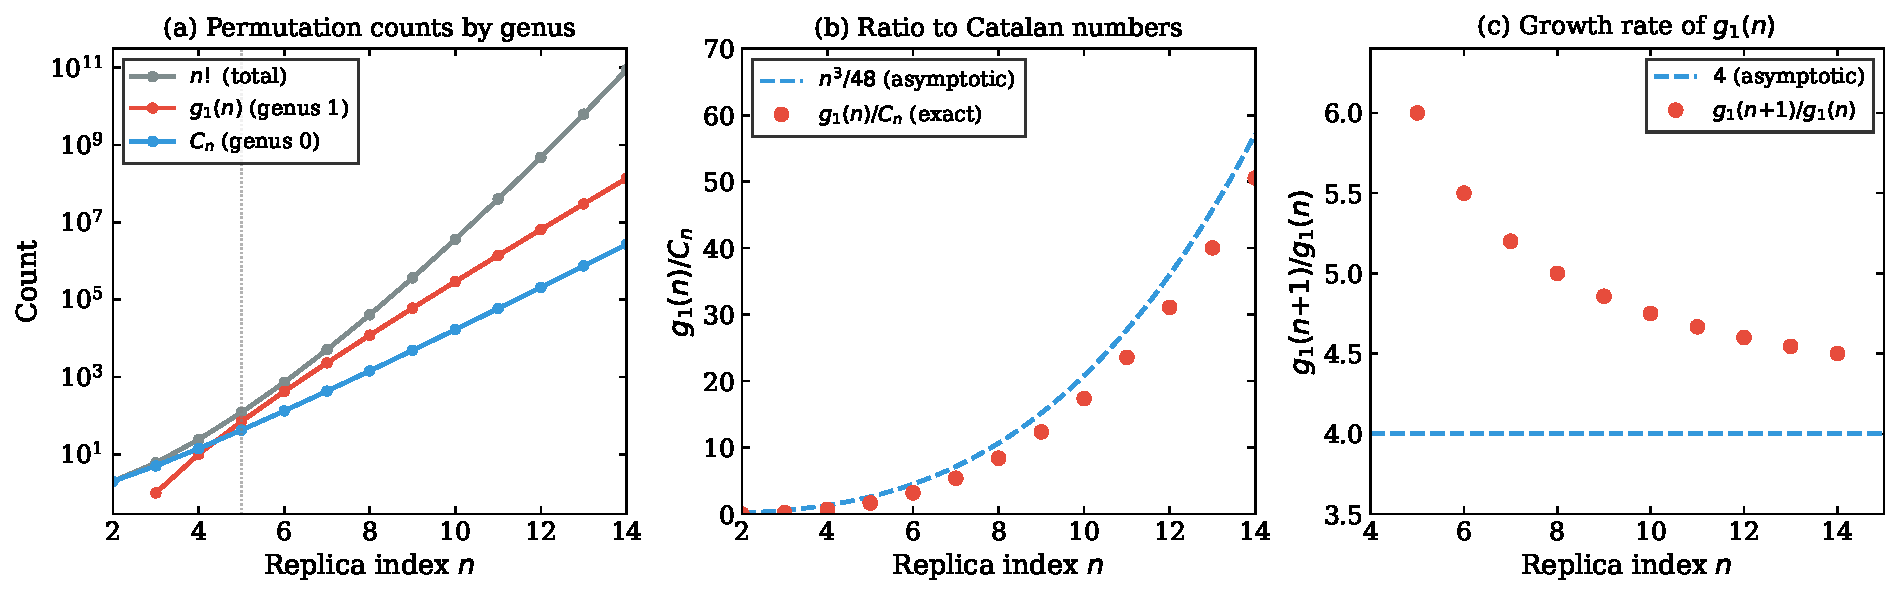
\includegraphics[width=\textwidth]{figures/output/fig10_genus1_growth.pdf}
\caption{Genus-one permutation counting.  (a) The counts $n!$, $g_1(n)$,
and $C_n$.  (b) The exact ratio $g_1(n)/C_n$ and its large-$n$ approximation
$n^3/48$.  (c) The ratio $g_1(n+1)/g_1(n)=2(2n-1)/(n-2)$ approaches four.
These are counts.  Their contributions to moments include dimension weights
and, for normalized states, the rising-factorial denominator.}
\label{fig10:genus1_growth}
\end{figure}

\subsection{Continuum handles, fluctuations, and QES corrections}

\subsubsection{The JT topology expansion}
For connected JT amplitudes with $b$ asymptotic boundaries, the perturbative
organization is~\citep{saadetal2019}
\begin{equation}
 Z_b^{\mathrm{conn}}(\beta_1,\ldots,\beta_b)
 \sim\sum_{g\geq0}e^{(2-2g-b)S_0}
 Z_{g,b}(\beta_1,\ldots,\beta_b).
 \label{eq10:genus_expansion}
\end{equation}
The coefficients include integrals over moduli spaces of hyperbolic surfaces,
with boundary wavefunctions fixed by the preparation.  Unlike the Wick genus
at fixed integer $n$, the continuum genus is unbounded at a fixed boundary
number.  In the JT matrix-integral description the perturbative coefficients
match a double-scaled spectral expansion.  Defining a nonperturbative theory
requires additional choices; a formal topology series alone does not fix a
unique completion.

Connectedness and genus are also different notions.  A genus-zero surface
can connect two or more boundaries and thus contribute to a connected
ensemble correlator.  A connected fluctuation does not automatically carry
the relative weight of an added handle.  Likewise, a one-loop determinant
about a fixed classical saddle is an expansion in fluctuations of fields on
that saddle, not a change in its topology.  These distinctions are needed
before importing powers of $e^{-S_0}$ into an entropy-variance calculation.

\subsubsection{What the Akers--Penington result establishes}
\citet{akerspenington2021} identify conditions in which the usual minimal-QES
formula needs leading-order corrections.  The issue concerns the bulk state
between competing surfaces, characterized by smooth min- and max-entropies.
It is not the genus-one coefficient in Eq.~\eqref{eq10:genus_one_count}.

A useful illustration is their mixture argument.  For
$\rho=p\rho_1+(1-p)\rho_2$, entropy concavity and the classical label bound
imply
\begin{equation}
 pS(\rho_1)+(1-p)S(\rho_2)
 \leq S(\rho)
 \leq pS(\rho_1)+(1-p)S(\rho_2)+h_2(p),
 \label{eq10:akers_penington}
\end{equation}
where $h_2(p)=-p\log p-(1-p)\log(1-p)$.  For fixed $p$, this uncertainty
is at most $\log2$.  A naive saddle prescription that instead differs from
the weighted component entropies by order $1/G_N$ contradicts these bounds.
The required correction is then leading in the semiclassical expansion,
even though no genus-one permutation has been invoked.  This example
explains why a state-sensitive QES correction cannot be identified with a
universal exponentially suppressed handle correction.

\subsubsection{What can be compared between models}
The permutation counts are mathematical constants in every genus.  The
physical weights assigned to replica components, the continuum moduli
integrals, normalization fluctuations, and state preparation are model data.
A comparison between two theories must calculate these data for the same
observable and regime.  The existence of a topological expansion, or an
agreement of leading thermodynamic entropies, does not establish equality of
their planar density or inequality of their first subleading coefficient.
The finite examples in the following sections demonstrate what spectra and
connected observables can distinguish without presupposing those uncomputed
gravity comparisons.

\section{What Entropies and Spectra Determine}
\label{sec11:universality_hierarchy}

The random-state calculation gives a precise answer to a specified
statistical question. It does not, by itself, identify the dynamics that
prepared the state. This section explains how much information is retained
by the different quantities used in that calculation. The distinction is
familiar from probability: a mean does not specify a distribution, and a
one-point distribution does not specify correlations. Here the random
objects are density matrices and their spectra.

We develop the distinction through elementary examples, including the
finite ensembles of Paper~III~\citep{wuebben2026paper3}. These examples
are useful because every state and every probability can be written down.
They do not assume a semiclassical approximation, an entropy expansion,
or a particular microscopic model of a black hole. Their role is to
identify which further calculations are required before an entropy result
can answer a question about ensembles or information recovery.

\subsection{From a density matrix to an entropy}
\label{subsec11:thermodynamics_analogy}

For a density matrix $\rho$ on $\mathbb C^d$, let
$\lambda_1,\ldots,\lambda_d$ be its eigenvalues, including zeros.
The spectral counting measure and its moments are
\begin{equation}
 \nu_\rho=\sum_{i=1}^d\delta_{\lambda_i},\qquad
 M_n(\rho)=\tr\rho^n=\int_0^1 x^n\nu_\rho(dx).
 \label{eq11:spectral_measure}
\end{equation}
The measure has mass $d$, while its first moment is one. The distinction
between these normalizations matters when comparing a density of
entanglement eigenvalues with a probability density. Entropy is another
linear functional of the counting measure:
\begin{equation}
 S(\rho)=-\int_0^1 x\log x\,\nu_\rho(dx),\qquad
 S_n(\rho)=\frac{\log M_n(\rho)}{1-n}.
 \label{eq11:renyi}
\end{equation}
Thus a spectrum determines all these entropies, but a single entropy
does not determine the spectrum. Even the full spectrum determines a
matrix only up to a unitary change of eigenvectors.

For an explicit example, choose $0<p<1$, $p\ne1/2$, and set
\begin{equation}
 \rho=\begin{pmatrix}p&0\\0&1-p\end{pmatrix},\qquad
 H=\frac1{\sqrt2}\begin{pmatrix}1&1\\1&-1\end{pmatrix},\qquad
 \rho'=H\rho H^\dagger.
 \label{eq11:isospectral_states}
\end{equation}
Every spectral entropy agrees. However, for the same physical observable
$Z=\operatorname{diag}(1,-1)$,
\begin{equation}
 \tr(\rho Z)=2p-1,\qquad \tr(\rho'Z)=0.
 \label{eq11:isospectral_observable}
\end{equation}
This is a change of state while the measurement basis is held fixed.
Rotating both the state and every observable would instead be a change
of representation. A radiation spectrum omits precisely this relation
between the eigenvectors and the accessible observables.

The analogy with thermodynamics has a limited but useful meaning. An
entropy is a coarse description of a state, just as an equation of state
is a coarse description of a material. Agreement of the coarse data is
compatible with disagreement of other data. It is not a theorem that
all microscopic theories agree on the coarse data: different Hamiltonians,
constraints, or preparations can already give different leading entropies.
The task is to state the data held fixed in each comparison.

\subsection{An averaged spectrum is not an ensemble of spectra}
\label{subsec11:four_levels}

Let $\rho$ now be random, with a specified probability distribution over
normalized density matrices on the same space. Then
\begin{equation}
 \overline\nu=\E\nu_\rho,\qquad
 \E M_n=\int x^n\overline\nu(dx),\qquad
 \E S=-\int x\log x\,\overline\nu(dx).
 \label{eq11:averaged_measure}
\end{equation}
These are one-point spectral data. They describe the expected number
of eigenvalues in any interval, not how eigenvalues occur together in
one realization. The two-point measure
$\E[\nu_\rho(dx)\nu_\rho(dy)]$ retains the latter information.
For example,
\begin{equation}
 \E[M_nM_\ell]
 =\iint x^ny^\ell\,\E[\nu_\rho(dx)\nu_\rho(dy)]
 \label{eq11:two_point_measure}
\end{equation}
cannot generally be recovered from $\overline\nu$.

This distinction persists even if all positive integer moments are
known exactly. Measures on $[0,1]$ are determined by their moments:
polynomials are uniformly dense among continuous functions, and equality
of their integrals therefore implies equality of the measures. For a
fixed $d$, the zeroth moment is supplied by $\overline\nu([0,1])=d$.
Consequently all $\E M_n$ determine $\overline\nu$. They do not
specify a probability measure on the space of spectra. To see the
missing information directly, it is enough to use four-dimensional
states.

\subsection{Two ensembles with exactly the same averaged spectrum}
\label{subsec11:formal_argument}

Set $c=1/4$ and choose $0\leq u<v<c$. Define
\begin{equation}
 \begin{aligned}
 L_u&=(c+u,c-u,c+u,c-u),\\
 L_v&=(c+v,c-v,c+v,c-v),\\
 L_{uv}&=(c+u,c-u,c+v,c-v).
 \end{aligned}
 \label{eq11:exact_spectra}
\end{equation}
All entries are positive and every row sums to one. Ensemble
$\mathcal A$ chooses the diagonal matrix with spectrum $L_u$ or $L_v$
with equal probabilities. Ensemble $\mathcal B$ always chooses the
spectrum $L_{uv}$. In both ensembles we then conjugate the state by an
independent Haar unitary in $U(4)$. The conjugation leaves every spectral
statistic unchanged and makes both averaged states equal to $I_4/4$.
It can be omitted if only spectral comparisons are of interest.

For any function $g$ defined on the four eigenvalue values, introduce
\begin{equation}
 a_g(t)=g(c+t)+g(c-t).
 \label{eq11:pair_statistic}
\end{equation}
The statistic $\tr g(\rho)$ has values $2a_g(u)$ and $2a_g(v)$ in
$\mathcal A$, and the single value $a_g(u)+a_g(v)$ in $\mathcal B$.
This proves the following exact comparison.

\begin{proposition}[Equal averaged spectra and unequal fluctuations]
\label{prop11:exact_ensembles}
The ensembles defined by \eqref{eq11:exact_spectra} satisfy
\begin{equation}
 \E_{\mathcal A}\tr g(\rho)=\E_{\mathcal B}\tr g(\rho)
 =a_g(u)+a_g(v).
 \label{eq11:linear_matching}
\end{equation}
For real-valued functions $g,h$, their covariances are
\begin{align}
 \Cov_{\mathcal A}(\tr g(\rho),\tr h(\rho))
 &=[a_g(u)-a_g(v)][a_h(u)-a_h(v)],
 \label{eq11:exact_covariance}\\
 \Cov_{\mathcal B}(\tr g(\rho),\tr h(\rho))&=0.
 \nonumber
\end{align}
In particular, their averaged spectral measures, all averaged replica
moments, and mean von Neumann entropies agree, while their purity and
entropy variances differ.
\end{proposition}

To verify the covariance, subtract the common mean. In $\mathcal A$
the two centered values of $\tr g(\rho)$ are
$\pm[a_g(u)-a_g(v)]$. The same sign occurs for $h$ in each realization,
so the product is the right-hand side of
\eqref{eq11:exact_covariance} in both realizations. Every spectral
statistic in $\mathcal B$ is constant. This derivation also shows that
the difference concerns correlations between eigenvalues, rather than
an error in matching the one-point density.

For purity, $a_g(t)=2(c^2+t^2)$, and hence
\begin{equation}
 \Var_{\mathcal A}(M_2)=4(u^2-v^2)^2,
 \qquad \Var_{\mathcal B}(M_2)=0.
 \label{eq11:purity_variance}
\end{equation}
For entropy define
$f(t)=-(c+t)\log(c+t)-(c-t)\log(c-t)$. Then
\begin{equation}
 \Var_{\mathcal A}(S)=[f(u)-f(v)]^2,
 \qquad \Var_{\mathcal B}(S)=0.
 \label{eq11:entropy_variance}
\end{equation}
Since $f'(t)=\log[(c-t)/(c+t)]<0$ for $0<t<c$, the first variance
is positive when $u<v$. There is no large-dimension limit in this
statement. Each matrix can be purified by an environment of dimension
four, so the example also defines ensembles of bipartite pure states.

\paragraph{A numerical example with rational eigenvalues.}
Take $u=0$ and $v=1/8$. The three spectra become
\begin{equation}
 L_0=(1/4,1/4,1/4,1/4),\quad
 L_{1/8}=(3/8,1/8,3/8,1/8),\quad
 L_{0,1/8}=(1/4,1/4,3/8,1/8).
 \label{eq11:rational_spectra}
\end{equation}
Their purities are $1/4$, $5/16$, and $9/32$, respectively. Averaging
the first two therefore gives the third, whereas their purity variance
is $1/1024$. Their common mean entropy is
\begin{equation}
 \E S=\frac52\log2-\frac38\log3,
 \qquad
 \Var_{\mathcal A}S
 =\frac14\left(\frac34\log3-\log2\right)^2.
 \label{eq11:example_values}
\end{equation}
The entropy of each averaged matrix is $\log4$. Thus even the entropy
of the averaged state and its difference from the mean entropy agree
between these ensembles. Section~\ref{sec12:annealed_quenched} will
relate their different entropy variances to finite-order R\'enyi
averages.

\begin{figure}[tbp]
 \centering
 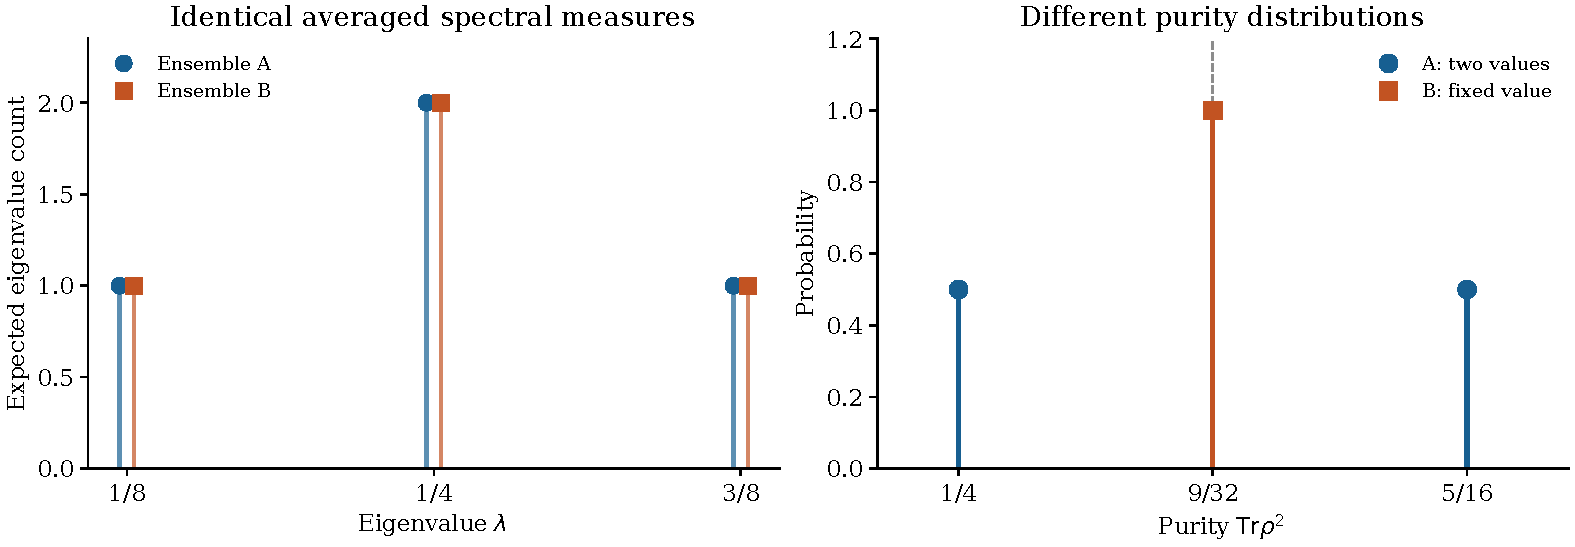
\includegraphics[width=\textwidth]{figures/output/fig11_exact_ensembles.pdf}
 \caption{The exact four-dimensional example
 \eqref{eq11:rational_spectra}. Left: the averaged eigenvalue counting
 measures agree; the markers are displaced horizontally only for
 visibility. Right: ensemble $\mathcal A$ has two equally probable
 purity values, whereas $\mathcal B$ has the constant purity $9/32$.
 Their means coincide, but their variances are $1/1024$ and zero.
 These are exact finite distributions, not random samples.}
 \label{fig11:exact_ensembles}
\end{figure}

\subsection{What a state design controls}
\label{subsec11:level_two}

Random circuits are often used to justify a random-state approximation.
The precise intermediate notion is a design. Let $\mathcal E$ be a
probability distribution on normalized pure states of
$\mathbb C^k\otimes\mathbb C^L$, and define its $n$-copy moment
operator by
\begin{equation}
 \Omega_{\mathcal E}^{(n)}
 =\E_{\mathcal E}(|\psi\rangle\langle\psi|)^{\otimes n}.
 \label{eq11:moment_operator}
\end{equation}
An exact projective state $t$-design reproduces the Haar moment
operators through order $t$. For approximate matching, specify the
error in trace norm:
\begin{equation}
 \epsilon_n=\|\Omega_{\mathcal E}^{(n)}
                  -\Omega_{\mathrm H}^{(n)}\|_1.
 \label{eq11:design_error}
\end{equation}
This definition is part of the assumption. A theorem about approximate
unitary designs stated in another norm must be translated before its
error can be substituted here. A unitary design acting on a fixed pure
input supplies a state design; one individual draw from the unitary
ensemble is not itself that design.

The replica permutation identity makes the consequence transparent.
Let $T_{R,n}$ cyclically permute the $n$ copies of the radiation factor
and act trivially on the remaining factors. Then
\begin{equation}
 \tr\rho_R^n=\tr\!\left[
 (|\psi\rangle\langle\psi|)^{\otimes n}T_{R,n}\right],
 \qquad \|T_{R,n}\|_\infty=1.
 \label{eq11:swap_identity}
\end{equation}
Subtracting the two ensemble averages and using
$|\tr AB|\leq\|A\|_1\|B\|_\infty$ gives
\begin{equation}
 \left|\E_{\mathcal E}M_n-\E_{\mathrm H}M_n\right|
 \leq\epsilon_n.
 \label{eq11:design_mp}
\end{equation}
A product $M_{n_1}\cdots M_{n_r}$ uses disjoint permutation cycles
and requires $n_1+\cdots+n_r$ copies. In particular, two-copy matching
controls mean purity, while four-copy matching controls its second
moment. Because $0\leq M_2\leq1$,
\begin{equation}
 \left|\Var_{\mathcal E}(M_2)-\Var_{\mathrm H}(M_2)\right|
 \leq\epsilon_4+2\epsilon_2.
 \label{eq11:design_variance}
\end{equation}
The second term bounds the difference between the squares of the means.
An exact two-design need not satisfy the four-copy condition.

The scale of the desired observable also matters. The natural scaled
spectral moment is $k^{n-1}M_n$, so its error is at most
$k^{n-1}\epsilon_n$. Recovering a Marchenko--Pastur moment as
$k,L\to\infty$ therefore requires control at that scale, in addition
to the corresponding Haar limit. Recovering a small covariance can
require substantially greater precision than recovering a leading mean.
The local random-circuit results of Brand\~ao, Harrow, and Horodecki
\citep{brandaoetal2016} give design statements under specified circuit
assumptions, with depth depending on design order. A scrambling-time
estimate alone supplies neither arbitrary-order design matching nor
these dimension-dependent error bounds.

\subsection{Passing from moments to an entropy limit}
\label{subsec11:level_three}

At fixed dimension, the compact support of the unscaled eigenvalues
makes the full moment problem well behaved. In a large-dimension
calculation the useful variables are instead $x_i=k\lambda_i$, with
empirical probability measure
$\mu_k=k^{-1}\sum_i\delta_{x_i}$. Now
\begin{equation}
 S(\rho_R)=\log k-\int x\log x\,\mu_k(dx).
 \label{eq11:scaled_entropy}
\end{equation}
A limiting law for $\mu_k$ must control this integral, including any
spectral tail. Weak convergence alone tests bounded continuous functions;
$x\log x$ is unbounded at infinity. It is therefore useful to state
one sufficient condition explicitly.

Suppose $\mu_k$ converges weakly in probability to a deterministic
measure $\mu$, and
$\sup_k\E\int x^2\mu_k(dx)<\infty$. For $K>e$,
\begin{equation}
 \int_{x>K}x\log x\,\mu_k(dx)
 \leq\frac{\log K}{K}\int x^2\mu_k(dx).
 \label{eq11:tail_bound}
\end{equation}
The expected right-hand side tends to zero as $K\to\infty$.
The integrand extends continuously to zero and is bounded below, so a
bounded truncation converges in probability and in mean. Removing the
truncation proves convergence of the entropy correction in
\eqref{eq11:scaled_entropy}. The same tail argument controls the
limiting integral. This is one route from a spectral law to entropy;
it displays the extra estimate that finitely many moment matches do
not automatically provide.

For the flat-weight Haar/Wishart model, the Marchenko--Pastur law and
Page's mean entropy are established benchmarks
\citep{marchenkopastur1967,page1993}. Their appearance in two calculations
is evidence of common state statistics in the stated regime. It does
not imply agreement of eigenvectors, finite-size covariances, or channel
matrix elements. Conversely, the presence of non-crossing partitions
alone does not force the Marchenko--Pastur law: different free cumulant
weights yield different moment sequences. Both the combinatorics and
the weights must be specified.

\subsection{A practical dictionary of the different questions}
\label{subsec11:dictionary}

Table~\ref{tab11:level_summary} summarizes implications established by
the definitions. Its rows are not a ranking of microscopic theories.
They indicate which data are discarded when a more detailed object is
replaced by a summary.

\begin{table}[tbp]
\centering
\caption{Data about a state, an ensemble, and a channel. A stronger
input in one row need not supply the data of another row.}
\label{tab11:level_summary}
\begin{adjustbox}{max width=\textwidth,center}
\begin{tabular}{p{0.23\textwidth}p{0.32\textwidth}p{0.34\textwidth}}
\toprule
Given data & What they determine & What remains unspecified \\
\midrule
One density matrix & All expectation values in that state & Its
preparation and channel action on other inputs \\[4pt]
Its full spectrum & Every spectral entropy & Eigenvectors relative to
physical observables \\[4pt]
Averaged spectral measure & All mean linear spectral statistics &
Covariances between those statistics \\[4pt]
Finite-order state design & Corresponding copy moments & Higher-order
errors, general entropy limits, and time correlations \\[4pt]
Full joint output for a maximally entangled reference input & The channel on every input & The physical
implementation and complexity of a decoder \\
\bottomrule
\end{tabular}
\end{adjustbox}
\end{table}

The last row will be derived in
Section~\ref{sec14:equilibrium_evaporation}. It is an important positive
result: sufficiently complete reference-assisted data do determine a
channel. The limitations established here concern particular incomplete
data, not an impossibility of learning quantum dynamics. Likewise,
extra spectral moments and covariances can distinguish specified models
when their predictions differ. What cannot be inferred is a universal
separation of broad gravitational programs before those predictions
have been calculated.

\paragraph{Exercises.}
For the spectra in \eqref{eq11:rational_spectra}, compute the common
third and fourth mean moments and verify that
$\E_{\mathcal A}M_2^2-\E_{\mathcal B}M_2^2=1/1024$.
Next omit the Haar conjugation and compare the two averaged matrices.
The averaged spectral measure still agrees, but equality of averaged
matrices no longer follows automatically. Finally, use
\eqref{eq11:exact_covariance} to calculate $\Cov(M_2,S)$ and explain
its sign: the more concentrated spectrum has higher purity and lower
entropy. These checks distinguish the role of spectral randomness
from the role of random eigenvectors.

\section{R\'enyi Averages and Entropy Fluctuations}
\label{sec12:annealed_quenched}

The terms annealed and quenched originate in problems where a logarithm
of a partition function is taken after or before an average over
disorder. The same ordering issue arises for replica moments. To use
the analogy, however, we must specify the normalized random quantity
inside the logarithm. The derivations below develop the finite-dimensional
identities used in Paper~III~\citep{wuebben2026paper3}.

An ensemble-averaged Page curve specifies a mean entropy.  It does not
specify how much the entropy varies between realizations, or how the
radiation states themselves vary.  These questions require different
observables.  We first distinguish the two customary orders of averaging
R\'enyi entropies, then relate their difference to a normalized replica
covariance.  The identities are elementary at finite dimension, but their
normalization and order of limits are essential when applying them to a
gravitational replica calculation.

Throughout this section, $\rho$ is a random density matrix on a fixed
$d$-dimensional Hilbert space, normalized separately in every realization:
$\rho\geq0$ and $\tr\rho=1$ almost surely.  The probability measure may
describe random states, couplings, circuits, or another specified
preparation.  Its mathematical existence does not determine which of
these physical interpretations is appropriate.  Logarithms are natural,
and $0\log0=0$.

\subsection{The two R\'enyi averages}
\label{subsec12:why_matters}

For real $n>1$, define the moment $M_n(\rho)=\tr\rho^n$ and the
annealed and quenched R\'enyi entropies by
\begin{align}
 A_n&=\frac{\log\E M_n}{1-n},
 \label{eq12:annealed_def}\\
 Q_n&=\frac{\E\log M_n}{1-n}=\E S_n(\rho).
 \label{eq12:quenched_def}
\end{align}
The labels refer only to the position of the logarithm relative to the
average.  In particular, $Q_n$ is still an ensemble average, rather than
the entropy of a distinguished member.  Concavity of the logarithm gives
\begin{equation}
 G_n:=Q_n-A_n
 =\frac{\log\E M_n-\E\log M_n}{n-1}\geq0.
 \label{eq12:gap_def}
\end{equation}
At a fixed order $n>1$, equality holds precisely when $M_n$ is constant
almost surely.  Constancy of one moment neither fixes the spectrum nor
identifies a Hamiltonian.  Even constancy of every spectral moment leaves
the eigenvectors undetermined.

\begin{proposition}[Von Neumann limit and its first correction]
\label{prop12:von_neumann_limit}
For any ensemble of normalized density matrices on a common
finite-dimensional Hilbert space,
\begin{equation}
 \lim_{n\to1}A_n=\lim_{n\to1}Q_n=\E S(\rho),
 \qquad S(\rho)=-\tr(\rho\log\rho).
 \label{eq12:common_limit}
\end{equation}
Moreover, as $t\to0$,
\begin{equation}
 G_{1+t}=\frac{t}{2}\Var[S(\rho)]+O(t^2).
 \label{eq12:gap_formula}
\end{equation}
The remainder is bounded uniformly over ensembles at fixed dimension.
\end{proposition}

\begin{proof}
Set $L_2(\rho)=\tr[\rho(\log\rho)^2]$.  Expansion of the normalized
moment gives
\begin{equation}
 M_{1+t}=1-tS+\frac{t^2}{2}L_2+O(t^3),\qquad
 \log M_{1+t}=-tS+\frac{t^2}{2}(L_2-S^2)+O(t^3).
 \label{eq12:moment_expansion}
\end{equation}
For $n$ in a compact interval contained in $(0,\infty)$, the functions
$x^n|\log x|^r$, extended by zero at $x=0$, are uniformly bounded on
$[0,1]$.  Summing over at most $d$ eigenvalues bounds the required
moment derivatives uniformly, including for rank-deficient states.
The moment also has a positive lower bound near $n=1$, so the logarithm
has uniformly bounded derivatives there.  These facts justify averaging
the Taylor expansions.  The linear coefficients of $\log\E M_{1+t}$
and $\E\log M_{1+t}$ are both $-\E S$.  Their quadratic coefficients
differ by $\Var(S)/2$.  Dividing their difference by $t$ proves the
claim.
\end{proof}

Thus there is no nonzero annealed--quenched von Neumann entropy gap
under these definitions.  Entropy fluctuations survive as the slope
of the finite-order R\'enyi gap.  The statement holds for each finite
dimension.  A large-dimension saddle approximation followed by analytic
continuation may require additional uniform estimates; such an
approximation does not change the exact finite-dimensional identity.
For an infinite-dimensional state space, the interchange of derivatives
and averages must instead be justified by suitable integrability bounds.

\subsection{Averaging a spectrum and averaging a state}
\label{subsec12:state_average}

Another nonnegative difference, often relevant to ensemble
interpretations, is
\begin{equation}
 \chi=S(\bar\rho)-\E S(\rho),\qquad \bar\rho=\E\rho.
 \label{eq12:holevo_quantity}
\end{equation}
This is the Holevo quantity of the state ensemble~\citep{holevo1973}.  It compares the
entropy of the averaged density operator with the mean entropy.  It
is not the $n\to1$ limit of $G_n$.  More explicitly,
\begin{equation}
 \chi=\E D(\rho\Vert\bar\rho),\qquad
 D(\rho\Vert\sigma)=\tr[\rho(\log\rho-\log\sigma)]\geq0,
 \label{eq12:relative_entropy_identity}
\end{equation}
where the support of $\rho$ lies in that of $\bar\rho$ almost surely.
Hence $\chi=0$ precisely when the density matrices themselves agree
almost surely.  This is a statement about the specified state ensemble,
not about whether an underlying theory is unique.

For comparison, let $\nu_\rho=\sum_{i=1}^d\delta_{\lambda_i(\rho)}$
be the eigenvalue counting measure.  Entropy is a linear functional of
this measure:
\begin{equation}
 -\int_0^1 x\log x\,\E\nu_\rho(dx)=\E S(\rho).
 \label{eq12:averaged_spectral_density}
\end{equation}
Averaging the spectral density before performing the entropy integral
therefore gives the mean entropy exactly.  The eigenvalues of
$\E\rho$ are generally not the averaged eigenvalue counting measure.
A concavity argument for density operators cannot be transferred to
this linear spectral integral.

An isospectral ensemble illustrates the distinction.  Fix a density
matrix $\rho_0$ and draw $\rho=U\rho_0U^\dagger$ with Haar-distributed
$U$.  All $M_n$, all R\'enyi entropies, and $S$ are deterministic, so
$G_n=0$ and $\Var(S)=0$.  Nevertheless $\bar\rho=I_d/d$ and
$\chi=\log d-S(\rho_0)$, which is positive unless $\rho_0$ is maximally
mixed.  For a pure $\rho_0$, $\chi=\log d$.  The radiation states can
therefore vary strongly while their entropies have no fluctuations at
all.  Conversely, a positive $G_n$ can arise from random preparation
within a fixed theory; it does not establish averaging over Hamiltonians.

\subsection{An exactly evaluated two-state ensemble}
\label{subsec12:two_state_example}

Consider the qubit ensemble
\begin{equation}
 \rho=\begin{cases}
 |0\rangle\langle0|,&\text{with probability }p,\\
 I_2/2,&\text{with probability }1-p,
 \end{cases}
 \qquad 0\leq p\leq1.
 \label{eq12:two_state_ensemble}
\end{equation}
Its moment has the two values $1$ and $2^{1-n}$.  All quantities in the
preceding discussion can therefore be calculated without a saddle
approximation:
\begin{align}
 Q_n&=(1-p)\log2,
 & A_n&=-\frac{\log[p+(1-p)2^{1-n}]}{n-1},
 \label{eq12:two_state_renyi}\\
 \Var(S)&=p(1-p)(\log2)^2,
 & \chi&=h_2\!\left(\frac{1+p}{2}\right)-(1-p)\log2,
 \label{eq12:two_state_variance}
\end{align}
where $h_2(x)=-x\log x-(1-x)\log(1-x)$ is binary entropy.
For $p=1/2$, the common von Neumann limit is $\log2/2$, whereas
$\chi=0.215762\ldots$.  At $n=2$,
$G_2=\log(3/4)+\log2/2=0.058892\ldots$.  The coefficient of $n-1$
in $G_n$ is $(\log2)^2/8=0.060057\ldots$.

\begin{figure}[htbp]
 \centering
 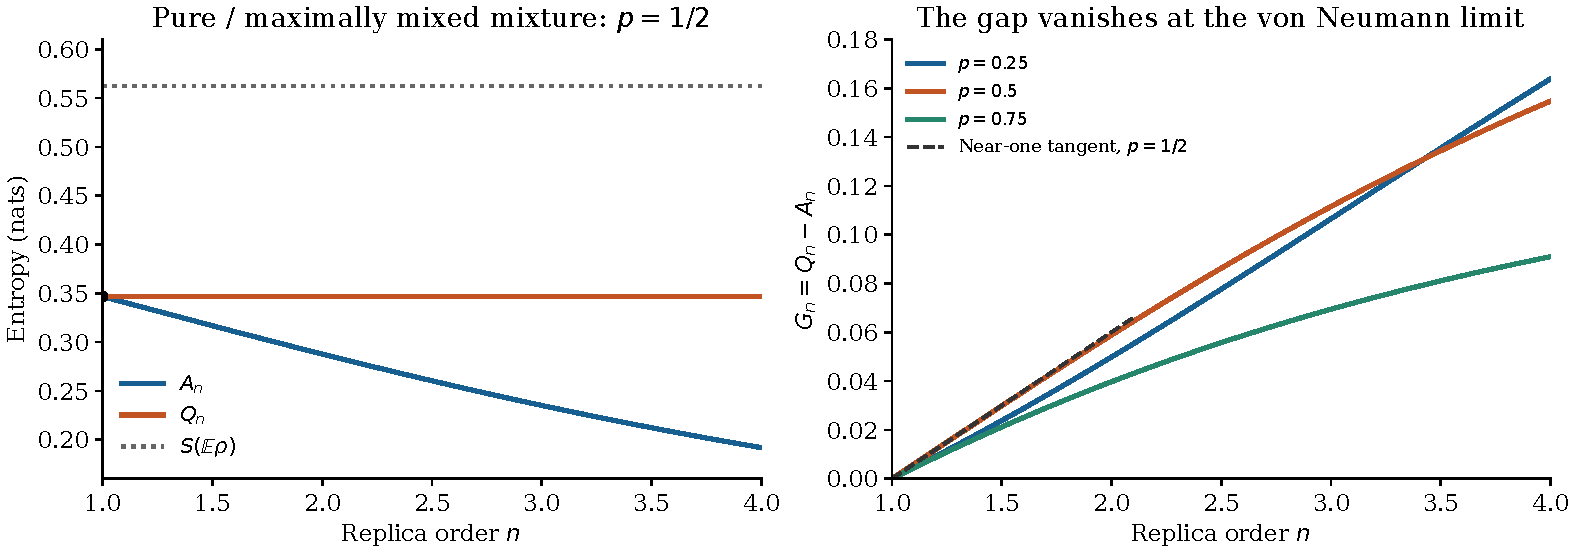
\includegraphics[width=\textwidth]{figures/output/fig12_annealed_quenched_gap.pdf}
 \caption{Exact averages for the qubit ensemble in
 \eqref{eq12:two_state_ensemble}.  Left: $A_n$ and $Q_n$ at $p=1/2$
 approach the same von Neumann limit; the entropy $S(\bar\rho)$ of the
 averaged state remains a different quantity.  Right: the nonnegative
 gap $G_n=Q_n-A_n$ for three mixing probabilities.  The dashed tangent
 at $p=1/2$ is $(n-1)\Var(S)/2$.  Every curve is obtained from
 \eqref{eq12:two_state_renyi}; no Page-time profile or gravitational
 fluctuation amplitude is assumed.}
 \label{fig12:annealed_quenched_gap}
\end{figure}

This example makes the observable distinction independent of any
large-entropy limit.  It also shows why the dependence of a fluctuation
observable on Page time cannot be inferred from Jensen's inequality.
The probability distribution and its time dependence would have to be
provided by a dynamical or state-preparation model.  A positive finite
R\'enyi gap, by itself, gives neither a universal peak position nor a
universal amplitude.

\subsection{Normalized replica covariances}
\label{subsec12:gap_computation}

The object that determines entropy fluctuations is the connected
moment
\begin{equation}
 C(n,\ell)=\E[M_nM_\ell]-\E M_n\,\E M_\ell.
 \label{eq12:connected_contrib}
\end{equation}
Normalization immediately implies $C(1,\ell)=C(n,1)=0$.  Differentiating
with respect to the two independent replica indices gives
\begin{equation}
 \left.\partial_n\partial_\ell C(n,\ell)\right|_{n=\ell=1}
 =\Var[S(\rho)].
 \label{eq12:entropy_covariance}
\end{equation}
Both identities are exact, with differentiation justified as in
Proposition~\ref{prop12:von_neumann_limit}.  The covariance contains
information absent from the one-point function $\E M_n$.  Knowing
the averaged spectral density, even exactly, does not determine it.

Proposition~\ref{prop11:exact_ensembles} gives an exact
finite-dimensional example of this separation.  Its two ensembles have
the same $\E M_n$ at every positive real order, the same mean entropy,
and the same averaged density matrix.  Consequently all their $A_n$
and their Holevo quantities agree.  One ensemble has a fixed spectrum,
whereas the other has two spectra with different entropies.  The latter
therefore has a nonzero entropy variance and a nonzero slope of $G_n$
at one.  Thus even complete knowledge of the one-point replica function
cannot reconstruct this fluctuation observable.

For a Haar-distributed pure state on $\mathbb C^m\otimes\mathbb C^b$,
let $\rho$ be the reduction to $\mathbb C^m$.  A useful exact comparison
is the purity variance~\citep{giraud2007}:
\begin{equation}
 \E M_2=\frac{m+b}{mb+1},\qquad
 C(2,2)=\frac{2(m^2-1)(b^2-1)}{(mb+1)^2(mb+2)(mb+3)}.
 \label{eq12:haar_purity_variance}
\end{equation}
We derive this formula below from normalized replica contractions.  It vanishes if either subsystem
is one-dimensional and, for $m=b\to\infty$, is $2m^{-4}+O(m^{-6})$.
The finite normalization factors contribute at the leading order of
the covariance, even though they only correct the leading mean purity
at subleading order.  A product of one-point approximations is therefore
insufficient for computing this variance.

\subsection{Concentration and its limits}
\label{subsec12:self_averaging}

For a specified order $n>1$, concentration of $M_n$ controls $G_n$.
Write $M_n=\mu_n(1+\delta_n)$, where $\mu_n=\E M_n$ and
$\E\delta_n=0$.  If $|\delta_n|\leq\eta<1$ almost surely, Taylor's
theorem applied to $-\log(1+\delta_n)$ gives the two-sided bound
\begin{equation}
 \frac{\E\delta_n^2}{2(n-1)(1+\eta)^2}
 \leq G_n\leq
 \frac{\E\delta_n^2}{2(n-1)(1-\eta)^2}.
 \label{eq12:gap_bound}
\end{equation}
Under the same condition the quadratic approximation is
\begin{equation}
 G_n=\frac{\Var(M_n)}{2(n-1)\mu_n^2}
 +O\!\left(\frac{\E|\delta_n|^3}{(n-1)(1-\eta)^3}\right).
 \label{eq12:relative_variance_expansion}
\end{equation}
These estimates state an explicit condition controlling the logarithm.
A small relative variance alone does not uniformly control rare events
with $M_n/\mu_n$ very close to zero as the dimension increases.  At
fixed dimension the lower bound $M_n\geq d^{1-n}$ supplies a bound,
but its constant need not remain useful in a large-dimension limit.

Near $n=1$, the numerator in the leading term of
\eqref{eq12:relative_variance_expansion} itself vanishes quadratically:
$\Var(M_{1+t})=t^2\Var(S)+O(t^3)$.  This restores the linear behavior
in \eqref{eq12:gap_formula}; treating that numerator as independent of
$n$ would give a spurious singularity.  Separately, an entropy variance
bound has the direct probabilistic consequence
\begin{equation}
 \Prob\{|S-\E S|\geq a\}\leq\frac{\Var(S)}{a^2},\qquad a>0.
 \label{eq12:entropy_concentration}
\end{equation}
This controls deviations of the entropy at the specified preparation
or time.  It does not imply concentration of the density operator, nor
simultaneous agreement of an entire trajectory without further temporal
control.

\subsection{Fluctuations within and between preparations}
\label{subsec12:conditional_variance}

An ensemble may contain more than one source of randomness.  Let
$\Theta$ denote a classical preparation parameter, such as an energy
window or the number of available environment states.  The law of total
variance gives
\begin{equation}
 \Var(S)=\E\bigl[\Var(S\mid\Theta)\bigr]
       +\Var\bigl(\E[S\mid\Theta]\bigr).
 \label{eq12:total_variance}
\end{equation}
The first term describes entropy fluctuations with the preparation held
fixed; the second describes variation of the conditional mean between
preparations.  They need not have the same size or the same dependence
on subsystem dimensions.  Matching one of these terms between models
does not match their total variance.

For example, keep the radiation dimension $m$ fixed and draw a positive
integer environment dimension $B$ from a specified distribution.
Conditional on $B=b$, draw a Haar bipartite state on
$\mathbb C^m\otimes\mathbb C^b$.  Every reduced state acts on the
same radiation Hilbert space, so the preceding finite-dimensional
identities apply even though the purifying space varies.  The exact
purity variance is
\begin{align}
 \Var(M_2)
 &=\E\!\left[
 \frac{2(m^2-1)(B^2-1)}{(mB+1)^2(mB+2)(mB+3)}\right]
 \notag\\
 &\quad+\Var\!\left(\frac{m+B}{mB+1}\right).
 \label{eq12:random_dimension_variance}
\end{align}
The second term is absent in a fixed-dimension comparison.  This
example supplies a precise probabilistic distinction between state
fluctuations at fixed dimension and fluctuations of the available number
of states.  It does not identify an arbitrary gravitational ensemble
with a mixture of Haar ensembles; that identification would require
the conditional state law as well as the distribution of $B$.

Conditioning also clarifies how thermodynamic broadening and entropy
fluctuations enter a comparison.  A fluctuating energy can change the
conditional mean entropy, while states within a narrow energy window
can still have a nonzero conditional variance.  A measured or computed
total variance alone cannot separate these contributions.  The
preparation or conditioning must be stated before assigning a physical
origin to either term.  All statements here concern a classical
probability distribution over density operators; replacing it by a
coherent superposition is a different state construction.

\subsection{Application to gravitational ensembles}
\label{subsec12:interpretation}

When a path integral initially constructs an unnormalized positive
operator $W$, the physical moment is
\begin{equation}
 M_n=\frac{\tr W^n}{(\tr W)^n}.
 \label{eq12:normalized_ratio}
\end{equation}
The average of this ratio generally differs from replacing its
denominator by $(\E\tr W)^n$.  In a covariance calculation, fluctuations
of the normalization can enter at the same order as the connected
numerator.  The normalization check $C(1,\ell)=0$ must hold before
using a replica derivative to infer entropy fluctuations.

Bousso and Miyaji~\citep{boussomiyaji2024} computed such fluctuations
in the PSSY model, explicitly retaining the fluctuating normalization.
Their calculation includes non-tubular and tubular contributions and
finds a difference from fixed-dimension Haar fluctuations after the
Page time, associated with fluctuations of the number of black hole
states in the chosen energy window.  This is an existing example of
information beyond the mean Page curve.  It is not a nonzero difference
between the two normalized von Neumann limits in
\eqref{eq12:common_limit}.  Moreover, connected replica geometries
need not introduce a handle: connectivity and genus are distinct
properties, and the suppression of a covariance must be calculated
in the specified model.

For a comparison between microscopic proposals, the ensemble measure,
normalization prescription, state preparation, and observable must
therefore be held fixed or related explicitly.  A nonzero covariance
can distinguish two specified preparations with different fluctuations.
Neither its presence nor its absence alone decides whether gravity is
described by one Hamiltonian.  The finite R\'enyi gap and entropy variance
provide useful additional data, while leaving the separate question of
recovering an unknown input to a channel analysis.


\subsection{A four-replica calculation of purity fluctuations}
\label{subsec12:four_replicas}

It is instructive to derive the Haar purity variance explicitly. This
also checks which replica data a fluctuation requires. In the following
calculation the radiation and environment dimensions are $k$ and $L$,
and $D=kL$. For a Haar vector on $\mathbb C^D$, its $r$-copy average is
\begin{equation}
 \E(|\psi\rangle\langle\psi|)^{\otimes r}
 =\frac1{(D)_r}\sum_{\pi\in S_r}U_\pi,
 \qquad (D)_r=D(D+1)\cdots(D+r-1).
 \label{eq12:haar_copy_average}
\end{equation}
This follows from unitary invariance: the average is the identity on
the symmetric subspace, divided by its dimension. The symmetrizer is
$r!^{-1}\sum_\pi U_\pi$, and its trace is
$\binom{D+r-1}{r}=(D)_r/r!$, giving the displayed normalization.
The identity is a finite-dimensional statement, before a planar
approximation.

Let $C(\pi)$ count the cycles of a permutation, including fixed points.
The radiation contraction for $M_2^2$ uses $\tau=(12)(34)$, so
\begin{equation}
 \E M_2^2=\frac{1}{(kL)_4}
       \sum_{\pi\in S_4}k^{C(\tau\pi)}L^{C(\pi)}.
 \label{eq12:four_replica_sum}
\end{equation}
The two disjoint cycles represent the two traces. This differs from a
single four-cycle, which would calculate $\E M_4$. Enumerating the
24 permutations gives the following polynomial:
\begin{align}
 \sum_{\pi\in S_4}k^{C(\tau\pi)}L^{C(\pi)}
 &=k^2L^4+2k^3L^3+k^4L^2+4kL^3\notag\\
 &\quad+10k^2L^2+4k^3L+2kL.
 \label{eq12:four_replica_polynomial}
\end{align}
For example, the identity permutation contributes $k^2L^4$, while
$\pi=\tau$ contributes $k^4L^2$. The coefficients sum to 24 when
$k=L=1$, as they must. Dividing by $(kL)_4$, subtracting
$[(k+L)/(kL+1)]^2$, and collecting terms gives
\begin{equation}
 \Var(M_2)=
 \frac{2(k^2-1)(L^2-1)}{(kL+1)^2(kL+2)(kL+3)}.
 \label{eq12:purity_variance_derived}
\end{equation}
This reproduces \eqref{eq12:haar_purity_variance} with $m=k,b=L$.
For two qubits, the mean purity is $4/5$ and its variance is $3/175$.
When either subsystem has dimension one, the variance vanishes exactly.
Both limits provide simple checks on the normalization.

At $k=L$, the large-dimension expansion is
\begin{equation}
 \E M_2=\frac2k-\frac2{k^3}+O(k^{-5}),\qquad
 \Var(M_2)=\frac2{k^4}+O(k^{-6}).
 \label{eq12:balanced_haar_asymptotic}
\end{equation}
The correction to the mean is small compared with the mean itself.
Nevertheless, its product with the leading mean contributes to the
square of the mean at order $k^{-4}$, the very order of the variance.
It is therefore inconsistent to retain connected terms of this size
while discarding the normalization corrections needed in the
subtraction. A leading spectral density is not sufficient for a
subleading fluctuation calculation.

\subsection{Interpreting vanishing and nonvanishing differences}
\label{subsec12:three_scenarios}

There are several distinct reasons why a difference can vanish. If
$\rho$ is deterministic, all ensemble fluctuations vanish. If its
spectrum is deterministic but its eigenvectors vary, every $G_n$ still
vanishes, although the Holevo quantity can be positive. If only one
moment is deterministic, $G_n$ vanishes at that order without fixing
all other spectral observables. Finally, the normalized von Neumann
annealed and quenched limits agree in every finite-dimensional
ensemble, including ones with large entropy variance. These are
mathematically different statements.

The converse implications are equally limited. A nonzero $G_2$
certifies fluctuations of purity in the specified ensemble; it does
not identify their origin. A nonzero entropy variance certifies variation
of entropy between preparations; it does not imply that every
measurement distinguishes those preparations. A nonzero Holevo quantity
certifies that the density matrices vary, even when every spectral
entropy is fixed. None of these statements alone determines whether
the Hamiltonian was fixed, randomly drawn, or incompletely specified.

\begin{table}[tbp]
\centering
\caption{Three nonnegative quantities and their distinct meanings.
All statements refer to normalized states in a common finite dimension.}
\label{tab12:three_scenarios}
\begin{adjustbox}{max width=\textwidth,center}
\begin{tabular}{p{0.24\textwidth}p{0.31\textwidth}p{0.34\textwidth}}
\toprule
Quantity & Vanishing condition & Information retained \\
\midrule
$G_n$ for fixed $n>1$ & $M_n$ is almost surely constant & Variation of
that particular moment \\[4pt]
$\Var(S)$ & $S$ is almost surely constant & Entropy fluctuations and
the slope of $G_n$ at one \\[4pt]
$S(\E\rho)-\E S(\rho)$ & $\rho$ is almost surely constant & Variation
of full density matrices, including eigenvectors \\
\bottomrule
\end{tabular}
\end{adjustbox}
\end{table}

\paragraph{Exercises.}
For the qubit ensemble \eqref{eq12:two_state_ensemble}, calculate
$C(n,\ell)$ directly and verify
$C(n,\ell)=p(1-p)(1-2^{1-n})(1-2^{1-\ell})$.
Differentiate at $n=\ell=1$ and recover its entropy variance. Next use
\eqref{eq11:exact_covariance} to calculate $C(n,\ell)$ for the two
four-dimensional ensembles. Their $\E M_n$ agree at every order, but
one covariance is zero and the other generally is not. Finally compare
an equally weighted ensemble of $|0\rangle$ and $|1\rangle$ with the
deterministic state $I_2/2$. Both averaged matrices are $I_2/2$, while
the mean entropies are zero and $\log2$. This last example makes clear
why specifying an averaged matrix also fails to specify an ensemble.

\section{Comparing Gravitational Descriptions}
\label{sec13:discriminating_proposals}

The examples above show that a radiation entropy, an averaged spectrum,
a fluctuation, and a channel recovery test answer different questions.
Applying these comparisons to gravity requires specifying the models
on both sides. The broad names used for approaches to the information
problem do not supply complete microscopic ensembles or evaporation
maps. They can also refer to different parts of one description:
a microscopic Hamiltonian, a family of states, a semiclassical
calculation, or a prescription for interior operators.

\subsection{What an entropy calculation establishes}

A calculation of $S(R)$ in a specified state constrains that state's
reduced density matrix. In gravity, the island prescription additionally
relates the entropy to a generalized-entropy extremization problem
\cite{engelhardtwall2015,penington2020,almheirietal2019}.
When accompanied by a code-subspace description and suitable
reconstruction assumptions, the calculation can support conclusions
about recoverable interior observables. Ref.~\cite{pssyetal2022}
contains an explicit Petz-map reconstruction argument in addition to
its replica entropy computation. These additional structures are not
encoded in the scalar function $S(R)$ alone.

This distinction prevents two opposite inferences. An entropy curve
that agrees with a unitary random-state benchmark does not uniquely
identify its preparation. Conversely, the existence of elementary
replacement-channel examples does not invalidate a reconstruction
argument that supplies more information than that curve. The examples
in section~\ref{sec14:equilibrium_evaporation} hold the specified
radiation data fixed while changing the channel on other inputs. A
gravity calculation that determines those additional inputs or their
reference correlations can exclude the replacement channel.

Matching the full sequence $\E\mathrm{Tr}\rho_R^n$ likewise has a
precise meaning. At fixed dimension it determines the averaged spectral
measure, since that measure is supported on a compact interval. It
does not determine a probability law on spectra. The finite-dimensional
construction in section~\ref{subsec11:formal_argument} demonstrates
this difference without an asymptotic approximation. A two-trace
correlator supplies additional data. Even those spectral data leave
operator matrix elements and the input dependence of the channel
unspecified.

\subsection{The objects supplied by different approaches}
\label{subsec13:five_proposals}

\subsubsection{Random-state and random-circuit models}
\label{subsec13:random_unitary}
A Haar-induced state is a precisely defined statistical model. It gives
finite-dimensional moments and fluctuations once the dimensions and
symmetry class are fixed. A random circuit can also specify an actual
channel and a time parameter. Its circuit architecture, depth, and
required design order then affect the approach to a design
\cite{brandaoetal2016}.
Replacing a circuit by a Haar state at every time retains a useful
benchmark but discards information about the temporal coupling of the
states. Section~\ref{sec14:equilibrium_evaporation} makes that distinction
explicit.

\subsubsection{Islands and replica wormholes}
\label{subsec13:island}
An island calculation is a prescription for entropies and related
observables within a gravitational setup. In the model of
ref.~\cite{pssyetal2022}, the replica sum can be compared with a
random-state spectral problem. In JT gravity, the matrix-integral
description computes particular ensemble quantities
\cite{saadetal2019}. Neither statement implies that every island
calculation is an ensemble of the same microscopic Hamiltonians.
Whether a boundary description is fixed or ensemble averaged is a
question about its definition and factorization properties
\cite{marolfmaxfield2020}. It cannot be settled by a von Neumann
annealed--quenched gap under the normalized definitions of
section~\ref{sec12:annealed_quenched}, because that gap vanishes.

\subsubsection{Microstate geometries and the fuzzball program}
\label{subsec13:fuzzball}
Microstate constructions seek a microscopic description of black-hole
states and their effective geometric properties. Mathur's analysis also
emphasizes restrictions on attempts to restore purity through small
corrections to a specified pair-creation process \cite{mathur2009}.
Explicit smooth supergravity solutions represent important families of
microstates in particular charge sectors; identifying them with every
black-hole microstate, or extrapolating their construction to a generic
nonextremal evaporating hole, requires further work
\citep{mathur2005,benawarner2008}. A radiation-spectrum comparison
requires a chosen family of states,
a probability distribution if an average is taken, and a coupling to
the radiation. The name of the program alone does not determine an
entanglement-spacing distribution or an entropy variance. In
particular, a claim about integrability of a Hamiltonian does not by
itself provide the local statistics of the reduced density matrix
produced in a specified evaporation experiment.

\subsubsection{State-dependent interior operators}
\label{subsec13:state_dependent}
State-dependent constructions concern the map between boundary
observables and interior operators in a specified class of states
\cite{papadodimasraju2013}. To compare them through outgoing radiation,
one must identify a boundary preparation and an observable whose
prediction differs. This is a question about which algebra is represented, on which states,
and with what accuracy. It does not prescribe a unique probability
distribution of outgoing states. A different representation of interior operators
need not change the radiation density matrix. If the same microscopic
state and outgoing algebra are used, all radiation entropies can agree
without resolving how the interior is represented.

\subsubsection{Geometric descriptions of entanglement}
\label{subsec13:erepr}
The ER=EPR proposal relates entanglement to geometric connections
\cite{maldacenasusskind2013}. By itself it does not specify a normalized
probability law for Hawking-radiation density matrices. Proposals relating complexity to geometric growth concern additional
observables and a definition of circuit cost
\citep{stanfordsusskind2014}. They do not specify an entanglement
spectrum from an entropy alone. A spectral or
recovery comparison therefore requires a concrete realization of the
proposal and a common set of observables. Its statements can coexist
with a microscopic unitary theory and with a semiclassical island
calculation. Treating these descriptions as mutually exclusive rows
with independently fixed numerical predictions would impose more
structure than their names provide.

\subsection{A comparison table with explicit status}
\label{subsec13:discrimination_matrix}

Table~\ref{tab13:discrimination_matrix} collects calculations rather than assigning
uncomputed predictions to broad programs. An equality in one row does
not imply equality in another. In particular, the energy ensemble and
accessible algebra must be held fixed in a channel comparison, while
normalization and matrix dimensions must be held fixed in a spectral
comparison.

\begin{table}[tbp]
\centering
\caption{Specified comparisons and the information they add. The first
two rows are calculated examples in this paper. The final two identify
gravity calculations from the literature or further model-dependent
questions; they are not predictions shared by every member of a named
approach.}
\label{tab13:discrimination_matrix}
\begin{adjustbox}{max width=\textwidth,center}
\begin{tabular}{p{0.24\textwidth}p{0.31\textwidth}p{0.35\textwidth}}
\toprule
Comparison & Data that agree & Additional distinction \\
\midrule
Isometry and replacement channel & All radiation states for one input
& Reference mutual information and recovery fidelity differ exactly \\[4pt]
Finite spectral ensembles & Averaged replica moments at every order
and mean entropy & Purity and entropy covariances differ exactly \\[4pt]
Gravitational entropy fluctuations & A specified mean Page curve
& Connected normalized replicas give model-dependent fluctuations;
ref.~\cite{boussomiyaji2024} computes an example \\[4pt]
Two proposed microscopic evaporation models & To be established for the
chosen states and couplings & Compute a common operator, reference, or
covariance observable before asserting a difference \\
\bottomrule
\end{tabular}
\end{adjustbox}
\end{table}

The last row is a research requirement. It is not an inference that all
microscopic descriptions must eventually disagree on one of the listed
quantities. Distinct descriptions of the same physics can agree on all
accessible observables. Conversely, two models can already differ in a
leading entropy curve if their state preparation, constraints, or
dynamics differ. There is no general rule that physically meaningful
differences begin only at a particular genus order.

\subsection{Precision, normalization, and accessible observables}

Three quantitative checks are needed before a small difference becomes
a useful comparison. First, the error of each calculation must be
smaller than the proposed distinction. Leading convergence to a common
spectral density does not control a finite-size covariance; the Haar
purity example illustrates the normalization terms required at that
order. Second, the same ensemble operation must be computed on both
sides. A ratio of averaged partition functions can differ from an
average of normalized density-matrix moments. Third, the observable
must belong to the algebra accessible in the proposed experiment.
An operator involving an external reference requires that reference
to be part of the state preparation.

Ensemble variance also differs from quantum measurement variance in a
single member. For an observable $O$ and states $\rho_\alpha$, the
variance in the average state decomposes as
\begin{align}
 \mathrm{Tr}(\overline\rho O^2)
 -\bigl[\mathrm{Tr}(\overline\rho O)\bigr]^2
 &=\E_\alpha\left[\mathrm{Tr}(\rho_\alpha O^2)
       -\mathrm{Tr}(\rho_\alpha O)^2\right]
 \nonumber\\
 &\quad+\Var_\alpha\left[\mathrm{Tr}(\rho_\alpha O)\right],
 \qquad \overline\rho=\E_\alpha\rho_\alpha.
 \label{eq13:variance_decomposition}
\end{align}
The two terms refer to repeated measurement within a preparation and
to variation between preparations. Determining which variation a
connected gravitational quantity represents requires an interpretation
of the ensemble. A single fixed Hamiltonian can still support an
ensemble of input states, random couplings in an experiment, or time
samples. A nonzero variance is therefore not, by itself, evidence for
an ensemble of Hamiltonians.


\subsection{How to formulate a comparison that can be calculated}
\label{subsec13:observable_ranking}

A useful comparison begins with a common preparation, not a list of
names for research programs. Suppose two models are claimed to describe
the same experiment. Specify a radiation algebra $\mathcal A_R$, an
initial-state space $A$, conserved charges, and a coupling to the
outgoing modes. If an average is involved, specify the probability
measure and which quantities are held fixed. One may then ask whether
the two models agree on
\begin{equation}
 \E\tr\rho_R^n,\qquad
 \Cov(\tr\rho_R^n,\tr\rho_R^\ell),\qquad
 \tr(\rho_R O),\qquad
 (\operatorname{id}_Q\otimes\mathcal N)(\rho_{QA}).
 \label{eq13:comparison_observables}
\end{equation}
These are, respectively, averaged spectral data, spectral correlations,
operator data, and reference-assisted channel data. There is no
universal ordering of their practical discriminatory power. Two models
may agree on every spectral quantity and differ in an operator matrix
element. They may agree on the full state for one input and differ on
another input. They may instead disagree already in the leading
entropy because they prepare different energy sectors.

For an example of the required precision, consider a proposed difference
$\delta V$ between two purity variances of order $k^{-4}$. An entropy
calculation accurate only up to order one cannot resolve that difference.
Even a moment approximation with absolute error $o(k^{-1})$ may be
insufficient. If the comparison uses approximate state designs, the
bound \eqref{eq11:design_variance} requires control of the relevant
two-copy and four-copy errors relative to $|\delta V|$. If it instead
uses a gravitational saddle expansion, every contribution at that order,
including normalization and the subtraction of disconnected terms,
must be included. The name of the approximation does not supply its
error estimate.

A further distinction concerns a family of states and a family of
Hamiltonians. A single Hamiltonian admits an ensemble of microcanonical
states, a thermal density matrix, different pure inputs, and time-dependent
preparations. Each can lead to different spectral fluctuations. Conversely,
an ensemble of Hamiltonians can have observables whose fluctuations
vanish in a specified limit. The physical interpretation of a covariance
therefore comes from the definition of the ensemble and the factorization
properties of the theory, not from the covariance's sign alone.

\subsection{Reconstruction, decoding, and geometric descriptions}
\label{subsec13:synthesis}

The information problem contains several related tasks. An entropy
calculation determines a scalar property of a reduced state. Entanglement
wedge reconstruction concerns the representation of a bulk algebra in
boundary degrees of freedom. A decoding problem asks for a channel that
recovers a specified input with a stated fidelity. An implementation
problem asks whether that decoder can be carried out with accessible
resources. These tasks can support one another, but the necessary
assumptions should remain visible when passing between them.

In particular, a mathematical decoder need not be computationally simple.
The Hayden--Preskill setup specifies an input, its reference, the prior
entanglement of the black hole, and access to early and late radiation
\citep{haydenpreskill2007}. The resulting recovery question contains
more data than a pure-input Page curve. Likewise, the Petz reconstruction
analysis of \citet{pssyetal2022} does not rest on the entropy graph alone.
The elementary counterexample in the next section therefore identifies
what the graph omits; it does not contradict a calculation that supplies
these additional channel or code-subspace data.

Geometric traversability is a separate issue. A traversable-wormhole
protocol specifies a coupling that changes the physical evolution;
Gao, Jafferis, and Wall provide a concrete example\citep{gaoetal2017}.
It is not a general consequence that implementing any decoder makes an
Einstein--Rosen bridge traversable. Similarly, a conjectural relation
between complexity and geometric growth does not by itself fix a
universal recovery time. A comparison must state the protocol, the
allowed interactions, and the notion of recovery before these times
can be equated.

These distinctions leave substantial room for useful calculations. The
normalized fluctuation calculation of Bousso and Miyaji is an existing
example where a gravitational ensemble supplies information beyond the
mean Page curve\citep{boussomiyaji2024}. Explicit microstate emission
models can be compared with statistical benchmarks when their state
sampling and radiation coupling are specified. A boundary construction
can be tested on a common code subspace through reference correlations.
The tutorial's finite examples provide checks on such calculations;
they are not replacements for carrying them out in gravity.

\paragraph{A comparison exercise.}
Suppose two calculations report the same $\E\tr\rho_R^n$ for every
integer $n\geq1$, in the same finite radiation dimension. List what
follows and what does not. The averaged spectral measures and mean
entropies agree. Purity variances need not agree, by
Proposition~\ref{prop11:exact_ensembles}. Matrix elements in a fixed
basis need not agree, by \eqref{eq11:isospectral_observable}. Finally,
even equality of all radiation matrix elements for one pure input does
not determine a channel on other inputs. The next section derives that
last statement and explains the positive role of full Choi tomography.

\section{From Equilibrium States to Evaporation Channels}
\label{sec14:equilibrium_evaporation}

The island calculations recover a turnover of the fine-grained radiation
entropy in controlled semiclassical settings
\citep{penington2020,almheirietal2019,almheirietal2020islands,pssyetal2022}.
This is an important constraint on the gravitational description. To state
what follows from the entropy curve alone, however, one must distinguish
the state produced by a specified preparation from the channel that acts
on unknown quantum information. The distinction is standard in quantum
information theory; the examples below make its consequences for a Page
curve explicit. They are finite-dimensional constructions, without a
claim to model local or energy-conserving gravitational dynamics.

\subsection{Entropy of a state and recovery of an input}
\label{subsec14:page_curve_meaning}

Let $A$ be an input system of dimension $D\geq2$. The emitted radiation
after $k$ steps is $R_k=b_1\otimes\cdots\otimes b_k$, and $B_k$ denotes
the remaining system. We use a finite-dimensional tensor factorization;
the identification of the corresponding radiation algebra in gravity is
an additional part of any gravitational application. For a pure state on
$B_kR_k$, the radiation entropy satisfies
\begin{equation}
 S(R_k)=-\tr(\rho_{R_k}\ln\rho_{R_k}),\qquad
 S(R_k)=S(B_k)\leq\min\{\ln d_{R_k},\ln d_{B_k}\}.
 \label{eq14:entropy_bound}
\end{equation}
Approach to this bound is a typicality statement, as in the random-state
calculation of Page~\citep{page1993}. Unitarity alone does not require an
initial rise, a unique maximum, or a particular turnover profile. A
unitary evolution may, for example, emit a product state for a specially
chosen input. A Page-like curve combines the endpoint purity expected
under complete unitary evaporation with assumptions about intermediate
entanglement.

Write $\Ncal_k$ for the completely positive trace-preserving channel from
$A$ to $R_k$. For a specified input $\psi_0=|\psi_0\rangle\langle\psi_0|$,
the entropy data are the numbers $S[\Ncal_k(\psi_0)]$. Information
recovery asks whether the action of $\Ncal_k$ on an input space can be
reversed, including when the input is entangled with a reference. A
single-input entropy curve is therefore a restriction of the data
relevant to recovery. The following elementary construction shows that
even complete knowledge of the radiation density matrices for that
input does not remove this restriction.

\begin{proposition}[Identical radiation histories for one input]
\label{prop14:channel_counterexample}
Let $R_N=b_1\otimes\cdots\otimes b_N$ have dimension at least $D$, and
let $|\Omega\rangle\in R_N$ and $|\psi_0\rangle\in A$ be normalized.
There exist an isometric channel $\Vcal$ and a constant-output channel
$\Ccal$ from $A$ to $R_N$ such that their reductions to every $R_k$
coincide on $\psi_0$. The channel $\Vcal$ has a left inverse on the
input space, whereas $\Ccal$ transmits no information about the input.
\end{proposition}

\begin{proof}
Extend $|\psi_0\rangle$ to an orthonormal basis of $A$, and extend
$|\Omega\rangle$ to an orthonormal set of $D$ vectors in $R_N$. Mapping
the first set to the second defines an isometry $V$ with
$V|\psi_0\rangle=|\Omega\rangle$. Define
\begin{equation}
 \Vcal(X)=VXV^\dagger,\qquad
 \Ccal(X)=\tr(X)\,|\Omega\rangle\langle\Omega|.
 \label{eq14:two_channels}
\end{equation}
Both maps are channels. For every $k$,
\begin{equation}
 \Vcal_k(\psi_0)=\Ccal_k(\psi_0)
 =\tr_{b_{k+1}\cdots b_N}|\Omega\rangle\langle\Omega|,
 \label{eq14:identical_marginals}
\end{equation}
where the subscript denotes restriction of the output to $R_k$.
The map $V^\dagger$ reverses $\Vcal$ on its image and extends to a
trace-preserving recovery channel on all of $R_N$. The output of
$\Ccal$ is independent of its input, so no recovery channel can reverse
it on a space of dimension greater than one.
\end{proof}

These are consistent histories of sequentially released subsystems:
prepare the full output once and emit the factors $b_1,\ldots,b_N$ in
order. Equation~\eqref{eq14:identical_marginals} equates every radiation
observable for the chosen input, including all R\'enyi entropies and
all matrix elements in a specified basis. It does not assert equality for
other inputs. In particular, it establishes a limitation of
single-preparation data rather than an obstruction to quantum channel
tomography.

\subsection{An exact rising and falling entropy curve}
\label{subsec14:bell_example}

An explicit choice of the output illustrates the proposition. Take
$N=2q$ qubits and pair qubit $j$ with qubit $q+j$:
\begin{equation}
 |\Omega\rangle
 =\bigotimes_{j=1}^{q}
 \frac{|0\rangle_j|0\rangle_{q+j}
       +|1\rangle_j|1\rangle_{q+j}}{\sqrt2}.
 \label{eq14:bell_output}
\end{equation}
For $k\leq q$, every emitted qubit is one half of a Bell pair whose
other half remains inside, so $\rho_{R_k}$ is maximally mixed. For
$k>q$, each additional emission completes one of those pairs. The
number of pairs crossing the radiation cut is therefore
$\min(k,2q-k)$, giving exactly
\begin{equation}
 S(R_k)=\min(k,2q-k)\ln2,\qquad 0\leq k\leq2q.
 \label{eq14:bell_curve}
\end{equation}
For six qubits, the entropies in units of $\ln2$ are
$0,1,2,3,2,1,0$. The final radiation state is pure. The proposition
produces this same trajectory under an information-preserving channel
and an input-erasing channel. The example is deliberately simple: its
linear branches and flat nonzero entanglement spectrum are not the
finite-size Haar profile. Any desired pure multipartite output,
including a Haar-typical one, can instead be used in the proposition.

The constant-output channel is often called a \emph{replacer channel}.
It has a globally isometric realization
\begin{equation}
 W|\psi\rangle_A
 =|\Omega\rangle_{R_N}\otimes|\psi\rangle_E,
 \qquad \Ccal(X)=\tr_E(WXW^\dagger),
 \label{eq14:replacer_dilation}
\end{equation}
where $E$ is an unobserved system of dimension $D$. The input has moved
to $E$; it has not been destroyed by the enlarged evolution. Thus the
example does not contradict unitarity of a closed system. It shows
that purity of the observed radiation does not certify that the
radiation contains the input. If one independently assumes that the
complete evolution is an isometry and that no complementary output
remains, recovery follows from those assumptions. They are not implied
by the curve. Equation~\eqref{eq14:replacer_dilation} also identifies
why this construction is not a model of complete black-hole
evaporation with a proven absence of remnants or hidden sectors.

\subsection{An external reference distinguishes the channels}
\label{subsec14:reference_test}

The relevant distinction can be measured by entangling the input with
a reference, as in quantum communication and the Hayden--Preskill
recovery problem~\citep{schumacher1996,haydenpreskill2007}. Let
\begin{equation}
 |\Phi_D\rangle_{QA}=\frac1{\sqrt D}
 \sum_{i=1}^{D}|i\rangle_Q|i\rangle_A,
 \qquad |\Psi_V\rangle=(I_Q\otimes V)|\Phi_D\rangle.
 \label{eq14:reference_input}
\end{equation}
The two final joint states are
\begin{equation}
 \rho_{QR_N}^{\Vcal}=|\Psi_V\rangle\langle\Psi_V|,
 \qquad
 \rho_{QR_N}^{\Ccal}=\frac{I_Q}{D}\otimes
 |\Omega\rangle\langle\Omega|.
 \label{eq14:reference_outputs}
\end{equation}
Consequently their mutual information, defined by
$I(Q:R)=S(Q)+S(R)-S(QR)$, is
\begin{equation}
 I(Q:R_N)_{\Vcal}=2\ln D,
 \qquad I(Q:R_N)_{\Ccal}=0.
 \label{eq14:reference_mutual_information}
\end{equation}
This is a different input preparation from the pure-state experiment
in equation~\eqref{eq14:identical_marginals}. For the reference-entangled
input, an information-preserving channel produces mixed radiation
entangled with $Q$; requiring its radiation entropy to vanish would
be the wrong recovery criterion.

One can also compare with the ideal encoded state through
\begin{equation}
 F_V(\Ncal)=\langle\Psi_V|
 (\operatorname{id}_Q\otimes\Ncal)
 (|\Phi_D\rangle\langle\Phi_D|)|\Psi_V\rangle.
 \label{eq14:encoding_fidelity}
\end{equation}
For the two channels,
\begin{equation}
 F_V(\Vcal)=1,
 \qquad F_V(\Ccal)=\frac1{D^2}.
 \label{eq14:reference_fidelities}
\end{equation}
Indeed, substituting the second state in
equation~\eqref{eq14:reference_outputs} gives
$D^{-2}\sum_i|\langle\Omega|V|i\rangle|^2=D^{-2}$, because
$|\Omega\rangle$ lies in the image of $V$. Applying a decoder that
inverts $V$ on this image gives the usual entanglement fidelity for
the maximally mixed input~\citep{schumacher1996}. Every decoder applied
to a replacer still produces a constant-output channel, whose
entanglement fidelity for that input is $D^{-2}$. These comparisons
distinguish transmission of quantum information from purification of a
specified output state without requiring a reconstruction of every
matrix element of the channel.

Full reference-assisted state tomography supplies a stronger positive
result. For the maximally entangled input above, define the normalized
Choi state of a channel $\Ncal:A\to R$ by
\begin{equation}
 J_{\Ncal}=(\operatorname{id}_Q\otimes\Ncal)
 (|\Phi_D\rangle\langle\Phi_D|)
 =\frac1D\sum_{i,j}|i\rangle\langle j|_Q
       \otimes\Ncal(|i\rangle\langle j|).
 \label{eq14:choi_state}
\end{equation}
The entire state $J_{\Ncal}$ determines the channel on every input:
\begin{equation}
 \Ncal(\omega)=D\,\mathrm{Tr}_Q
       [(\omega^{\mathsf T}\otimes I_R)J_{\Ncal}],
 \label{eq14:choi_inversion}
\end{equation}
where the transpose is taken in the basis defining $|\Phi_D\rangle$.
This is the standard channel-state correspondence \cite{choi1975}; the
formula follows by contracting the displayed matrix units. Thus one
suitably entangled preparation with complete joint-state information
can determine a channel. Entropy or selected reference correlators
retain only part of that information. The single-input counterexample
concerns a fixed unentangled input, and does not apply to tomography of
$J_{\Ncal}$.

\subsection{Consistency of successive radiation states}
\label{subsec14:nested_channels}

Use the finite-dimensional notation of
Section~\ref{sec14:equilibrium_evaporation}. A sequential isometric model
has maps
\begin{equation}
\begin{aligned}
 U_k&:A\longrightarrow B_k\otimes R_k,\qquad
 W_{k+1}:B_k\longrightarrow B_{k+1}\otimes b_{k+1},\\
 U_{k+1}&=(W_{k+1}\otimes I_{R_k})U_k,
\end{aligned}
 \label{eq14:sequential_isometries}
\end{equation}
with the tensor factors reordered where necessary. Ancillas in a
specified initial state may be included in $B_k$. The corresponding
radiation channels $\Ncal_k(X)=\tr_{B_k}(U_kXU_k^\dagger)$ obey
\begin{equation}
 \tr_{b_{k+1}}\Ncal_{k+1}(X)=\Ncal_k(X)
 \quad\hbox{for every input operator }X.
 \label{eq14:channel_consistency}
\end{equation}
This equation assumes that emitted modes are no longer acted upon;
equivalently, their freely evolving observables can be described in an
interaction picture. It is a constraint on channels and their joint
outputs, not merely on the values of their entropies.

For example, assigning $|0\rangle\langle0|$ to the first emitted qubit
and a Bell state to the first two emitted qubits gives two valid
density matrices, both pure. They cannot be the successive radiation
states of this model: tracing the second qubit out of the Bell state
gives $I/2$, not $|0\rangle\langle0|$. Sampling an unrelated Haar state
at each instant similarly does not establish
equation~\eqref{eq14:channel_consistency}. A dynamical random-state
approximation must explain how the jointly distributed states are
generated, even when each individual state has the expected marginal
statistics. The constructions in
Proposition~\ref{prop14:channel_counterexample} do satisfy this
consistency condition because they release subsystems of a single
prepared output.

Entropy inequalities give a weaker, useful necessary condition. Since
$R_{k+1}=R_kb_{k+1}$,
\begin{equation}
 S(R_{k+1})-S(R_k)=S(b_{k+1}|R_k),\qquad
 |S(R_{k+1})-S(R_k)|\leq\ln\dim b_{k+1}.
 \label{eq14:entropy_increment}
\end{equation}
The bound follows from subadditivity and the Araki--Lieb inequality.
A decreasing radiation entropy requires negative conditional entropy
of the new emission given the earlier radiation. In the Bell-pair
example, the increment is $+\ln2$ for the first $q$ emissions and
$-\ln2$ for the last $q$. This accounts for the turnover through
explicit early--late correlations, while remaining insufficient to
decide whether those correlations encode the initial input.

\subsection{Fixed total energy does not fix the black-hole energy}
\label{subsec14:energy_constraints}

Energy conservation constrains the joint state rather than assigning
zero variance to the energy of every subsystem. For subsystems described
by an additive Hamiltonian, a fixed-total-energy space has the
decomposition
\begin{equation}
 \Hcal_{E_{\mathrm{tot}}}
 =\bigoplus_E\Hcal_B(E)\otimes
                  \Hcal_R(E_{\mathrm{tot}}-E).
 \label{eq14:energy_shell}
\end{equation}
A state in this space can have an arbitrary distribution $p_E$ over
the allowed black-hole energies. Orthogonality of the radiation energy
sectors makes its reduced state block diagonal,
\begin{equation}
 \rho_B=\bigoplus_Ep_E\rho_{B,E},\qquad
 S(\rho_B)=-\sum_Ep_E\ln p_E+
                     \sum_Ep_E S(\rho_{B,E}).
 \label{eq14:sector_entropy}
\end{equation}
The first term is the entropy of the energy-sector probabilities, and
the second is the mean entropy within sectors. Neither is fixed by
specifying $E_{\mathrm{tot}}$ alone. Sampling assumptions and dynamics
determine $p_E$.

The simplest illustration uses two qubits with excitation energy
$\varepsilon$. The pure state
\begin{equation}
 |\psi_p\rangle
 =\sqrt p\,|1\rangle_B|0\rangle_R
  +\sqrt{1-p}\,|0\rangle_B|1\rangle_R
 \label{eq14:fixed_energy_example}
\end{equation}
has exact total energy $\varepsilon$, but
\begin{equation}
 \Var(E_B)=\varepsilon^2p(1-p),\qquad
 S(\rho_R)=-p\ln p-(1-p)\ln(1-p).
 \label{eq14:fixed_energy_variance}
\end{equation}
These are quantum fluctuations in one pure state; no average over
Hamiltonians is involved. In an evaporating system, uncertainty in the
remaining energy can likewise be correlated with the energy already
emitted. Isolation does not justify replacing that distribution by a
delta function at the mean black-hole energy.

The equilibrium counterpart further specifies the distribution. If
states in a narrow total-energy shell are sampled with microcanonical
weights, then the energy-sector probabilities are proportional to the
product of the two densities of states. The stable quadratic expansion
of this product, derived in Section~\ref{subsec09:central_distinction},
gives a variance of $E_B/T$ equal to the effective heat capacity
$(C_B^{-1}+C_R^{-1})^{-1}$. Fixing $E_B$ itself removes this exchange
fluctuation, whereas fixing $E_B+E_R$ does not. Because the two
subsystem energies are anticorrelated, the variance of the difference
between their thermodynamic entropies is four times the individual
entropy variance at leading Gaussian order~\citep{wuebben2026paper2}.
These thermodynamic entropies count states; they are distinct from
the fine-grained entropies in equation~\eqref{eq14:sector_entropy}.
An outgoing flux need not be in equilibrium with the remaining black
hole, so the equilibrium law cannot be assigned to evaporation without
justifying its exchange and sampling assumptions.

\subsection{A fluctuation width is not an evaporation timescale}
\label{subsec14:instantaneous_approximation}

Replacing an equilibrium parameter by a function of time does not
determine either the radiation channel or its preparation law.
Suppose, more specifically, that an instantaneous approximation has
identified two entropy branches with mean difference $\Delta(t)$ and
a distribution for their centered difference. Let its width in entropy
units be $\sigma_\Delta(t)$, and assume that the distribution and the
local entropy formula vary slowly while $\Delta(t)$ crosses zero.
If $\dot\Delta(t_*)\ne0$, linearization supplies the estimate
\begin{equation}
 \tau_{\mathrm{round}}\sim
 \frac{\sigma_\Delta(t_*)}{|\dot\Delta(t_*)|},
 \qquad \Delta(t_*)=0.
 \label{eq14:time_width}
\end{equation}
Its coefficient depends on the convention used to define a crossover
width. The estimate requires the fluctuation law and
$\dot\Delta$ to change little over $\tau_{\mathrm{round}}$; it also
requires relaxation to justify the instantaneous description. If the
crossing is tangent or relaxation is slow, the linear estimate fails.
A thermodynamic variance alone supplies none of these dynamical
conditions.

Similarly, a Marchenko--Pastur law at a fixed dimension ratio follows
from a stated random-state or covariance model, not from time
dependence of the ratio. Emission spectra, conserved charges and
energy-dependent matrix elements can change the allowed states and
their weights. In a gravitational application the relevant entropy
branches must be derived from the generalized entropy prescription;
they cannot always be replaced by logarithms of unweighted Hilbert
space dimensions. The calculations of
Sections~\ref{sec07:free_probability} and
\ref{sec08:area_fluctuations} then provide conditional local models
whose assumptions can be tested in the dynamical setting. They do
not imply a universal sharp transition for isolated evaporation.

\subsection{What a dynamical comparison should specify}
\label{subsec14:dynamical_target}

A comparison between two evaporation models should fix the input
space, the preparation, the emitted radiation algebra, and the
conservation laws. It should state whether averages concern initial
states, dynamics, or Hamiltonians, and identify any degrees of freedom
that are traced out at the endpoint. Within that common setup, one
can compare radiation moments at specified times, their connected
fluctuations, and correlations between emissions. Reference-assisted
recovery tests then address the dependence on unknown inputs, as in
Section~\ref{subsec14:reference_test}. Computational difficulty of a
decoder is a further question beyond its mathematical existence
\citep{haydenpreskill2007}.

The gravitational calculation has additional responsibilities: a
specified coupling to a bath or asymptotic radiation region, a
semiclassical state and its backreaction, and a justification of the
entropy prescription in the regime being studied. These conditions
are realized to different degrees in existing island models
\citep{almheirietal2019,almheirietal2020islands}.
They should be evaluated model by model. Neither a fixed Hamiltonian
nor fixed total energy eliminates all statistical fluctuations, and
agreement of time-indexed equilibrium entropies does not establish
agreement of quantum channels. These distinctions specify the
additional calculations needed to connect the controlled examples in
this paper to microscopic black-hole information recovery.


\subsection{A two-qubit reference calculation}
\label{subsec14:qubit_reference}

The general channel construction can be checked with two emitted qubits.
Let the input be one qubit and define the isometry
\begin{equation}
 V|0\rangle=|\Phi^+\rangle,
 \qquad V|1\rangle=|\Phi^-\rangle,
 \qquad |\Phi^\pm\rangle=\frac{|00\rangle\pm|11\rangle}{\sqrt2}.
 \label{eq14:qubit_isometry}
\end{equation}
The two Bell states are orthogonal, so $V^\dagger V=I_2$.
Compare $\mathcal V(X)=VXV^\dagger$ with
$\mathcal C(X)=\tr(X)|\Phi^+\rangle\langle\Phi^+|$.
For input $|0\rangle$, both produce the same complete radiation state.
After the first emission the state is $I_2/2$, and after the second it
is $|\Phi^+\rangle\langle\Phi^+|$. Their radiation entropies are
therefore exactly $0,\log2,0$ at the three cuts.

The channels differ for other inputs. For
$|+\rangle=(|0\rangle+|1\rangle)/\sqrt2$,
\begin{equation}
 V|+\rangle=|00\rangle,
 \qquad \mathcal C(|+\rangle\langle+|)
       =|\Phi^+\rangle\langle\Phi^+|.
 \label{eq14:qubit_other_input}
\end{equation}
Measuring $Z$ on the first emitted qubit gives expectation one for
$\mathcal V$ and zero for $\mathcal C$. The common history of the
chosen input did not determine even this simple response to a different
preparation.

For a reference-entangled input
$(|00\rangle_{QA}+|11\rangle_{QA})/\sqrt2$, the isometric output is
\begin{equation}
 |\Psi_V\rangle_{QR}
 =\frac{|0\rangle_Q|\Phi^+\rangle_R
             +|1\rangle_Q|\Phi^-\rangle_R}{\sqrt2}.
 \label{eq14:qubit_reference_state}
\end{equation}
Its entropies satisfy $S(Q)=S(R)=\log2$ and $S(QR)=0$, so
$I(Q:R)=2\log2$. The replacement channel gives
$(I_Q/2)\otimes|\Phi^+\rangle\langle\Phi^+|$, with
$S(QR)=S(Q)=\log2$ and $S(R)=0$, so $I(Q:R)=0$.
The larger radiation entropy in the first case is a consequence of
successful reference entanglement, not a failure of information
recovery. A purity criterion appropriate to an unentangled input must
therefore not be imposed on this different experiment.

For completeness, the Choi reconstruction formula can be checked at
the level of matrix units. Substituting
$J_{\mathcal N}=D^{-1}\sum_{ij}|i\rangle\langle j|\otimes
\mathcal N(|i\rangle\langle j|)$ into
\eqref{eq14:choi_inversion} gives
\begin{equation}
 D\tr_Q[(\omega^{\mathsf T}\otimes I)J_{\mathcal N}]
 =\sum_{ij}\omega_{ij}\mathcal N(|i\rangle\langle j|)
 =\mathcal N(\omega).
 \label{eq14:choi_contraction}
\end{equation}
Thus complete tomography includes the off-diagonal input operators
that a single pure-input history leaves untested. The use of a
maximally entangled input also explains why the factor $D$ and the
transpose appear. Measuring only the eigenvalues or entropy of the
Choi state would discard some of these matrix elements and would not
in general reconstruct the channel.

\begin{table}[tbp]
\centering
\caption{Static data and additional requirements for a dynamical
interpretation. The requirements are conditional on the intended
observable; they are not claims that every evaporation model has the
same fluctuation law.}
\label{tab14:equilibrium_vs_evaporation}
\begin{adjustbox}{max width=\textwidth,center}
\begin{tabular}{p{0.25\textwidth}p{0.3\textwidth}p{0.33\textwidth}}
\toprule
Static calculation & What can be retained & Additional dynamical input \\
\midrule
Haar/MP state statistics & A conditional state benchmark & A justified
state law and consistent successive marginals \\[4pt]
Energy-sector distribution & A law under its preparation assumptions &
Emission dynamics and exchange or sampling assumptions \\[4pt]
Entropy crossover width & Width in entropy units & Branch velocity,
relaxation, and variation of the law during the crossing \\[4pt]
Pure-input entropy trajectory & Entropies of that preparation & Channel
action on an input space and reference correlations \\[4pt]
A mathematical decoder & Recovery with its stated error & Access to
radiation, allowed operations, and computational cost \\
\bottomrule
\end{tabular}
\end{adjustbox}
\end{table}

\section{Further Calculations and Open Questions}
\label{sec14:research_program}

The preceding sections separate several calculations that can be pursued
without assuming that all microscopic descriptions share one universal
hierarchy. The most direct extensions begin with a normalized state
model and then add one piece of information that its mean entropy
omits. The examples also provide elementary consistency checks for
more difficult gravitational computations.

\subsection{Six concrete targets}
\label{subsec14:six_targets}

\paragraph{1. Normalized spectral correlations in a common preparation.}
A useful extension of a one-point replica calculation is
$C(n,\ell)$ for independently variable replica indices. The normalization
checks $C(1,\ell)=C(n,1)=0$ must be satisfied, and the mixed derivative
at one must equal the entropy variance. The purity calculation in
Section~\ref{subsec12:four_replicas} is a finite-dimensional reference.
For a gravitational model, one should specify the energy window and
separate fluctuations in the number of available states from
fluctuations conditional on that number. Bousso and Miyaji's PSSY
calculation already implements a nontrivial part of this program
\citep{boussomiyaji2024}; it is a starting point for comparisons, not
an uncomputed prediction.

\paragraph{2. Finite-order R\'enyi averages with controlled continuation.}
The objects to compare are $A_n$ and $Q_n$ at $n>1$, or the covariance
that controls their near-one difference. Their normalized von Neumann
limits agree. A calculation of a nonzero limit should therefore first
check its normalization, its definition of entropy, and the order of
its large-dimension and replica limits. A controlled result would state
the approximation error on an interval near one and identify any
nonuniform behavior. The qubit figure in
Section~\ref{sec12:annealed_quenched} provides a direct check on the
sign and slope conventions.

\paragraph{3. Conditional spectra in fluctuating energy sectors.}
Thermodynamics specifies sector weights only after the preparation is
chosen. It does not specify whether sector contributions are visible
as orthogonal blocks in the radiation algebra. A useful calculation
would hold the energy law fixed while deriving the overlaps and the
conditional state law. One can then compare the entropy of the
resulting state with the average of conditional entropies, rather than
identifying them by assumption. The diagonal and planar distinctions
in Paper~I~\citep{wuebben2026paper1} give a controlled example of this
issue. Its extension to another gravity model requires its own
spectral equation and state normalization.

\paragraph{4. Regular and critical reservoir limits.}
At a regular stable saddle, a finite reservoir gives the effective
capacity $(C_B^{-1}+C_R^{-1})^{-1}$. Near a critical saddle the quadratic
approximation can fail, and a non-Gaussian law must be derived before
an entropy average is evaluated. Paper~II~\citep{wuebben2026paper2}
provides conditional finite-reservoir and quartic calculations.
Extending them to evaporation requires a dynamical justification of
local equilibration, the energy-sector law, and the branch variables.
One should compute their covariance as well as their marginal
variances: the difference of two correlated entropy branches can have
a very different width from either branch separately.

\paragraph{5. Consistent evaporation channels.}
A time-indexed family of density matrices should be replaced or
supplemented by maps satisfying
\eqref{eq14:channel_consistency}. A tractable circuit with energy or
charge conservation is one possible starting point. One can test its
single-time moments, correlations between emissions, and recovery of
an input entangled with a reference. The absence of an unobserved
endpoint system is an additional physical assumption that must be
established if final radiation purity is used as evidence of complete
recovery. The Bell-pair construction demonstrates why that assumption
cannot be read off an entropy graph.

\paragraph{6. A matched comparison of two gravitational descriptions.}
Choose an observable, a preparation, and an approximation accuracy
before comparing two descriptions. The target may be a connected
replica moment, an operator matrix element, or a recovery fidelity.
The comparison becomes informative when both calculations use the
same radiation algebra and conserved charges and have errors smaller
than the claimed difference. If the descriptions are dual accounts of
the same physics, agreement may be the appropriate result. If they
are different models, a discrepancy must be traced to an identified
assumption rather than assigned to the label of a research program.

\subsection{How the checks fit together}
\label{subsec14:decision_tree}

For a spectral calculation, begin with positivity and normalization of
the proposed state. Identify whether the calculated object is a moment
of a normalized state, a ratio of averages, or an average of ratios.
Then specify whether the result is exact at finite dimension or only
at a fixed order of an asymptotic expansion. If the question concerns
fluctuations, compute the relevant products of traces and their
subtractions at the same accuracy. If it concerns entropy, justify the
replica derivative or the spectral integral, including the required
limit interchange.

For a dynamical calculation, add the input space and sequential output
maps. Check compatibility of their reduced states and the treatment of
already emitted modes. State whether the test uses a fixed pure input,
a distribution of inputs, or an input entangled with a reference. An
entropy curve, an average fidelity, and full channel tomography are
different data sets; choosing one should match the physical question.
Finally, separate the existence of a recovery channel from the resources
needed to implement it.

These checks do not reduce the importance of the Page curve. They
explain how its information can be extended. A controlled entropy
calculation, a normalized covariance, and a reference-assisted channel
test each add a definite statement. Combining them in a specified
gravitational model is a substantive research objective, with the
finite examples serving as transparent tests of what each calculation
has and has not determined.

\part{Conclusion and Perspective}
\section{Conclusions}
\label{sec15:summary}
\label{sec15:punchline}

\subsection{From entanglement to the replica spectrum}
\label{subsec15:chain}

A pure state of a composite system can have mixed reduced states. Hawking
radiation entangled with interior partners therefore need not violate
unitarity while the black hole remains present. The difficulty arises when
the semiclassical description is extrapolated through complete evaporation,
leaving mixed radiation and no remaining purifier. The Bell-pair and
partial-trace calculations isolate the quantum structure of that argument.

Ryu--Takayanagi surfaces, their covariant generalization, and quantum extremal
surfaces relate entropy to bulk area and bulk entanglement
\citep{ryutakayanagi2006,hubenyetal2007,engelhardtwall2015}. In the evaporating
models of \citet{penington2020,almheirietal2019,almheirietal2020islands},
competing entropy branches produce a Page transition. Replica wormholes give
a path-integral derivation \citep{pssyetal2022,ahmstetal2020}. These are
results for specified gravitational preparations and observables.

Random-state models make a substantial part of the spectral calculation
explicit. Exact normalized Haar moments distinguish the random trace from
its mean. Their large-dimension expansion is organized by permutations,
and its leading flat-weight sector by non-crossing partitions. The
resolvent gives the Marchenko--Pastur distribution, whose entropy recovers
the large-dimension limit of Page's result
\citep{page1993,marchenkopastur1967}. Free probability supplies the moment
calculus; the gravitational weighted problem requires additional spectral
input \citep{wang2023,chengetal2024}. A common planar organization does
not require all preparations to have the same spectrum.

The finite-dimensional calculation also clarifies subleading terms.
Absence of a crossing permutation does not imply absence of a normalized
observable's correction at the corresponding order: the normalization
itself contributes. Adding a handle to a gravitational surface differs from
evaluating a fluctuation determinant on a fixed surface. Neither operation
can be identified without a derivation with the leading QES corrections
studied by \citet{akerspenington2021}.

\subsection{Thermodynamic preparation and entropy averaging}
\label{subsec15:thermodynamics}

For conditional states $\rho_x$ with probabilities $p_x$, the average
$\sum_xp_x S(\rho_x)$ need not equal $S(\sum_xp_x\rho_x)$. Orthogonal
sectors contribute a classical mixing entropy; overlapping sectors require
spectral overlap information. A diagonal approximation therefore needs a
definition of the conditional states and of what happens to their labels
when they are averaged. Paper I's comparison with planar spectral entropy
is an application of this distinction \citep{wuebben2026paper1}.

Once an averaged-minimum model is specified, its smoothing can be computed.
A Gaussian branch difference gives the familiar normal-density and
normal-distribution functions. A stable canonical saddle can produce this
law, but identifying its variance with a black-hole heat capacity uses a
local thermodynamic expansion. If both entropy branches fluctuate, their
covariance contributes to the variance of their difference.

At a quartic critical saddle the scale and profile change. A finite
reservoir can compete with the quartic term and restore a quadratic
contribution. Paper II makes these model regimes explicit
\citep{wuebben2026paper2}, complementing fixed-energy entanglement
calculations \citep{murthysrednicki2019} and fixed-area holographic
analysis \citep{marolfwangwang2020}. Fixed total energy does not fix each
subsystem energy. An ensemble name alone does not determine a
radiation-entropy width without identifying the state and observable.

\subsection{Spectra, ensembles, and information recovery}
\label{subsec15:observables}

The final chapters give concrete examples of different information supplied
by different observables. Two ensembles can have identical averaged spectral
measures, all averaged moments, and mean entropy, while their entropy and
purity fluctuations differ. A one-point spectral average records the
frequency of individual eigenvalues, but not their grouping into
realizations. Connected moments contain information about this grouping.

For normalized finite-dimensional states, annealed and quenched R\'enyi
entropies have the same von Neumann limit. Their finite-order difference is
still informative: close to replica number one, its leading coefficient is
half the entropy variance. Entropy of the averaged density matrix is a
third quantity. These distinct averaging operations answer distinct questions.

At the dynamical level, knowing the radiation state for one preparation
need not identify a channel. Agreement on that input leaves the action on
other inputs and coherent superpositions undetermined. Reference-system
correlations reveal the difference. Conversely, a full normalized Choi state
determines a finite-dimensional channel when its input and output spaces
and basis convention are fixed. This specifies which stronger data settle
the identification problem.

These constructions do not establish equality of predictions between two
particular theories of gravity. They specify the comparisons needed for
such a conclusion. Fuzzballs, islands, random dynamics, state-dependent
reconstruction, and ER=EPR address different aspects of the information
problem and are not automatically mutually exclusive. A quantitative
comparison fixes a common preparation and observable and then tests whether
the predictions differ within their stated approximations.

\subsection{Further calculations}
\label{subsec15:outlook}

The remaining gravitational questions can now be formulated precisely.
One can compare a diagonal conditional-entropy average with a planar
spectral calculation for the same preparation. One can compute normalized
connected replicas, including normalization corrections, to determine
fluctuations in a specified ensemble. One can derive the joint
fluctuations of competing generalized entropies instead of inferring them
from one heat capacity. Finally, one can test whether a sequence of
equilibrium approximations comes from a consistent evaporation channel
and which reference correlations that channel preserves.

The tutorial develops the calculations needed to formulate these questions
and finite models in which several can be answered completely. Their
gravitational applications require the corresponding preparation, spectral
weights, and dynamics. Keeping these inputs explicit allows the Page curve
to serve both as a quantitative entropy calculation and as a starting point
for further tests of information recovery.


\appendix

\section{Notation and Conventions}
\label{app:notation}

This appendix collects the notation and conventions used throughout the paper.
We work exclusively in natural units,
\begin{equation}
  \hbar = c = k_{\mathrm{B}} = 1\,,
  \label{eq16:natural_units}
\end{equation}
so that energy, mass, temperature, and inverse length all share the same
dimension, and the Bekenstein--Hawking entropy is the dimensionless ratio
$A/4G_N$.  Entropies are measured in \emph{nats} (base-$e$), not bits (base-2);
the conversion is $1\;\text{bit} = \ln 2\;\text{nats}$.  All logarithms are
natural unless stated otherwise.

\subsection{Black hole variables}

\begin{table}[ht]
\centering
\renewcommand{\arraystretch}{1.35}
\begin{adjustbox}{max width=\textwidth,center}
\begin{tabular}{@{}lp{10.6cm}@{}}
\hline
\textbf{Symbol} & \textbf{Definition} \\
\hline
$S_{\mathrm{BH}}$ &
  Bekenstein--Hawking entropy of the black hole, $S_{\mathrm{BH}} = A/(4G_N)$.
  Treated as a function of time during evaporation. \\
$S_0$ &
  Extremal (topological) entropy: the zero-temperature piece of
  $S_{\mathrm{BH}}$.  In JT gravity, $S_0 = \phi_0/(4G_N)$
  where $\phi_0$ is the constant (topological) piece of the dilaton;
  the boundary value $\phi_b$ instead sets the Schwarzian coupling $C$
  (Appendix~\ref{app:jt_gravity}). \\
$S_{\mathrm{rad}}$ &
  Coarse-grained (thermodynamic) entropy of the Hawking radiation. \\
$\Delta$ &
  Entropy-branch difference: $\Delta \equiv S_{\mathrm{rad}} - S_{\mathrm{BH}}$
  in the illustrative evaporation model. Other preparations define their
  branch entropies locally. \\
$t_P$ &
  Page time: the instant at which $S_{\mathrm{rad}} = S_{\mathrm{BH}}$, i.e.\
  $\Delta = 0$. \\
$\beta$ &
  Inverse Hawking temperature, $\beta = 1/T_H$. \\
$C_B$ (or $C_V$) &
  Geometric heat capacity of the black hole at constant volume (or at fixed charge, as
  appropriate).  For a Schwarzschild black hole in four dimensions,
  $C_V = -8\pi G_N M^{2}$. \\
$\sigma$ &
  Standard deviation of the explicitly specified entropy variable or
  difference of branch entropies.  At a stable regular canonical saddle,
  linearization gives $\operatorname{Var}S_{\mathrm{BH}}\simeq C_B$.
  For a finite reservoir, the corresponding energy variance is
  $T^2C_{\mathrm{eff}}$, where
  $C_{\mathrm{eff}}=(C_B^{-1}+C_R^{-1})^{-1}>0$.
  Correlations enter the variance of a difference of branch entropies. \\
\hline
\end{tabular}
\end{adjustbox}
\caption{Black-hole thermodynamic variables.  Geometric heat capacities,
canonical energy variances, and entropy-coordinate variances agree only under
the ensemble and linearization assumptions stated in the text.}
\label{tab16:bh_variables}
\end{table}

\subsection{Hilbert space dimensions and the ratio \texorpdfstring{$\gamma$}{gamma}}

The Haar benchmark uses finite-dimensional subsystems.  In gravity these
dimensions represent specified effective state counts, for example in a chosen
energy window; the full JT Hilbert space is not finite-dimensional.

\begin{table}[ht]
\centering
\renewcommand{\arraystretch}{1.35}
\begin{adjustbox}{max width=\textwidth,center}
\begin{tabular}{@{}lp{10.6cm}@{}}
\hline
\textbf{Symbol} & \textbf{Definition} \\
\hline
$\mathcal{H}_{\mathrm{rad}}$ &
  Hilbert space of the radiation subsystem; dimension $k$. \\
$\mathcal{H}_{\mathrm{BH}}$ &
  Hilbert space of the finite black-hole factor; dimension $L$. \\
$k$ &
  $\dim\mathcal{H}_{\mathrm{rad}}$.  Fixed in each static calculation;
  written $k(t)$ when a dynamical model specifies its time dependence. \\
$L$ &
  $\dim\mathcal{H}_{\mathrm{BH}}$.  The flat-weight scan can vary $k$ at
  fixed $L$; an evaporation model may instead have $L(t)$.
  The convention $L=e^{S_0}$ is a simplified state count, not a general JT identity. \\
$\gamma$ &
  Ratio $\gamma \equiv k/L$, as in Section~\ref{sec07:free_probability}.
  Free cumulants have a replica-order subscript, $\kappa_m$; surface gravity
  is denoted $\kappa$ in the main text and $\kappa_s$ in this appendix.
  The Page transition occurs at $\gamma = 1$. \\
$\eta$ &
  Symmetric ratio $\eta=\min(k,L)/\max(k,L)\leq1$, used for the smaller-side
  spectral density and entropy. \\
$D$ &
  In Haar moment formulas, $D=kL$ and $(D)_n$ is its rising factorial.
  In Section~\ref{sec14:equilibrium_evaporation}, $D$ instead denotes the
  channel input dimension. Thermodynamic $N$ is defined locally. \\
\hline
\end{tabular}
\end{adjustbox}
\caption{Hilbert space dimension variables.}
\label{tab16:hilbert_variables}
\end{table}

\subsection{Combinatorial notation}

\begin{table}[ht]
\centering
\renewcommand{\arraystretch}{1.35}
\begin{adjustbox}{max width=\textwidth,center}
\begin{tabular}{@{}lp{10.6cm}@{}}
\hline
\textbf{Symbol} & \textbf{Definition} \\
\hline
$C_n$ &
  Catalan number: $C_n = \frac{1}{n+1}\binom{2n}{n}$.  Counts the non-crossing
  partitions of $\{1,\dots,n\}$, i.e.\ $C_n = |\mathrm{NC}(n)|$.  The first
  values are $C_0 = 1$, $C_1 = 1$, $C_2 = 2$, $C_3 = 5$, $C_4 = 14$,
  $C_5 = 42$. \\
$N(n,j)$ &
  Narayana number: $N(n,j) = \frac{1}{n}\binom{n}{j}\binom{n}{j-1}$
  for $1 \le j \le n$.
  Counts non-crossing partitions of $\{1,\dots,n\}$ with exactly $j$ blocks.
  Satisfies $\sum_{j=1}^{n} N(n,j) = C_n$. \\
$c_n$ &
  Cyclic permutation $(1\,2\cdots n)$ imposed by an $n$th trace moment. \\
$\mathrm{NC}(n)$ &
  Lattice of non-crossing partitions of $\{1,\dots,n\}$. \\
$\mathrm{Kr}(\pi)$ &
  Kreweras complement of $\pi \in \mathrm{NC}(n)$. \\
$\mu_{\mathrm{NC}}$ &
  M\"obius function on the lattice $\mathrm{NC}(n)$. \\
\hline
\end{tabular}
\end{adjustbox}
\caption{Combinatorial notation.}
\label{tab16:combinatorial_notation}
\end{table}

\subsection{Random matrix notation}

\begin{table}[ht]
\centering
\renewcommand{\arraystretch}{1.35}
\begin{adjustbox}{max width=\textwidth,center}
\begin{tabular}{@{}lp{10.6cm}@{}}
\hline
\textbf{Symbol} & \textbf{Definition} \\
\hline
$W$ &
  Wishart matrix: $W = X X^{\dagger}$, where $X$ is a $k \times L$ matrix
  with i.i.d.\ mean-zero entries of variance $1/L$
  (Eq.~\eqref{eq16:wishart_def}). This is $1/L$ times the unit-variance
  Wishart matrix denoted $W$ in Section~\ref{sec06:replica_wormholes}. \\
$\rho_{\mathrm{MP}}(\lambda)$ &
  Marchenko--Pastur distribution with ratio parameter $\gamma = k/L$. \\
$\lambda_{\pm}$ &
  Marchenko--Pastur edges: $\lambda_{\pm} = (1 \pm \sqrt{\gamma})^{2}$. \\
$G(z)$ &
  Stieltjes transform of a spectral distribution:
  $G(z) = \int \frac{\rho(\lambda)\,d\lambda}{z - \lambda}$. \\
$R(z)$ &
  $R$-transform: $R(z) = G^{\langle -1\rangle}(z) - 1/z$, where
  $G^{\langle -1\rangle}$ is the functional inverse of $G$. \\
$\Phi(z)$, $\phi(z)$ &
  Standard normal CDF and PDF, respectively. \\
\hline
\end{tabular}
\end{adjustbox}
\caption{Random matrix and probability notation.}
\label{tab16:rmt_notation}
\end{table}

\subsection{Sign conventions and metric signature}

We adopt the ``mostly plus'' metric signature $(-,+,+,+)$.  The Riemann tensor
is defined by
\begin{equation}
  R^{\alpha}{}_{\beta\gamma\delta}\, V^{\beta}
  = \bigl(\nabla_{\gamma}\nabla_{\delta}
  - \nabla_{\delta}\nabla_{\gamma}\bigr) V^{\alpha}\,,
  \label{eq16:riemann_convention}
\end{equation}
the Ricci tensor by $R_{\mu\nu} = R^{\alpha}{}_{\mu\alpha\nu}$, and the
Einstein equations read
\begin{equation}
  G_{\mu\nu} + \Lambda\, g_{\mu\nu} = 8\pi G_N\, T_{\mu\nu}\,.
  \label{eq16:einstein_eq}
\end{equation}
In two-dimensional JT gravity these reduce to the dilaton equation of motion
reviewed in Appendix~\ref{app:jt_gravity}.


\section{The Non-Crossing Partition Lattice}
\label{app:nc_partitions}

Non-crossing partitions, introduced by Kreweras \cite{kreweras1972} and
developed into a central pillar of free probability by
Speicher~\cite{speicher1994,speicher1997}, organize the planar flat-weight
replica contractions of Section~\ref{sec07:free_probability}.  This appendix provides a
self-contained development.

\subsection{Definition and first examples}

\begin{quote}
\textbf{Definition.}
A \emph{partition} of the set $[n] = \{1,2,\dots,n\}$ is a collection
$\pi = \{B_1, B_2, \dots, B_j\}$ of non-empty, pairwise disjoint subsets
(\emph{blocks}) whose union is $[n]$.  The partition $\pi$ is
\emph{non-crossing} if, whenever $a < b < c < d$ and $a,c \in B_i$ and
$b,d \in B_k$, we have $i = k$.  Equivalently, when the elements of $[n]$ are
placed in order around a circle and the elements of each block are connected by
convex hulls, no two blocks cross.
\end{quote}

We denote the set of all non-crossing partitions of $[n]$ by $\mathrm{NC}(n)$.
Its cardinality is the Catalan number $C_n$.  For small $n$ the enumeration
proceeds as follows.

\medskip
\noindent
\textbf{$n=1$:}  There is a single partition $\{1\}$; it is trivially
non-crossing.  $|\mathrm{NC}(1)| = C_1 = 1$.

\medskip
\noindent
\textbf{$n=2$:}  The two partitions of $\{1,2\}$ are $\bigl\{\{1,2\}\bigr\}$
and $\bigl\{\{1\},\{2\}\bigr\}$.  Both are non-crossing.
$|\mathrm{NC}(2)| = C_2 = 2$.

\medskip
\noindent
\textbf{$n=3$:}  Of the five partitions of $\{1,2,3\}$, all are non-crossing
(there are not enough elements to create a crossing).
$|\mathrm{NC}(3)| = C_3 = 5$.  The partitions, grouped by number of blocks, are:
\begin{itemize}
  \item 1~block:  $\{1,2,3\}$.
  \item 2~blocks: $\{1,2\}\{3\}$, \ $\{1,3\}\{2\}$, \ $\{1\}\{2,3\}$.
  \item 3~blocks: $\{1\}\{2\}\{3\}$.
\end{itemize}

\medskip
\noindent
\textbf{$n=4$:}  Of the 15 set partitions of $\{1,2,3,4\}$, exactly 14 are
non-crossing.  The single crossing partition is $\bigl\{\{1,3\},\{2,4\}\bigr\}$,
whose blocks interleave.  $|\mathrm{NC}(4)| = C_4 = 14$.

\medskip
\noindent
\textbf{$n=5$:}  $|\mathrm{NC}(5)| = C_5 = 42$.

\subsection{The Narayana refinement}

The Narayana number $N(n,j)$ counts the non-crossing partitions of $[n]$ with
exactly $j$ blocks:
\begin{equation}
  N(n,j) = \frac{1}{n}\binom{n}{j}\binom{n}{j-1}\,,
  \qquad 1 \le j \le n\,.
  \label{eq16:narayana_def}
\end{equation}
These satisfy the Catalan sum rule
\begin{equation}
  \sum_{j=1}^{n} N(n,j) = C_n = \frac{1}{n+1}\binom{2n}{n}\,,
  \label{eq16:catalan_sum}
\end{equation}
and the \emph{Narayana duality}
\begin{equation}
  N(n,j) = N(n,\, n+1-j)\,,
  \label{eq16:narayana_duality}
\end{equation}
reflecting the bijection that sends each non-crossing partition to its
Kreweras complement (see below).

\begin{table}[ht]
\centering
\renewcommand{\arraystretch}{1.3}
\begin{adjustbox}{max width=\textwidth,center}
\begin{tabular}{@{}c|ccccccc|c@{}}
\hline
$n \backslash j$ & 1 & 2 & 3 & 4 & 5 & 6 & 7 & $C_n$ \\
\hline
1 & 1 &   &   &   &   &   &   & 1 \\
2 & 1 & 1 &   &   &   &   &   & 2 \\
3 & 1 & 3 & 1 &   &   &   &   & 5 \\
4 & 1 & 6 & 6 & 1 &   &   &   & 14 \\
5 & 1 & 10 & 20 & 10 & 1 &   &   & 42 \\
6 & 1 & 15 & 50 & 50 & 15 & 1 &   & 132 \\
7 & 1 & 21 & 105 & 175 & 105 & 21 & 1 & 429 \\
\hline
\end{tabular}
\end{adjustbox}
\caption{Narayana numbers $N(n,j)$.  The manifest duality
$N(n,j) = N(n,n+1-j)$ is visible as the left--right symmetry of each row.
The row sums give Catalan numbers $C_n$.}
\label{tab16:narayana_table}
\end{table}

\subsection{Lattice structure}

The set $\mathrm{NC}(n)$ carries a natural partial order: $\pi \le \sigma$ if
every block of $\pi$ is contained in a block of $\sigma$ (i.e.\ $\pi$ is a
\emph{refinement} of $\sigma$).  Under this order, $\mathrm{NC}(n)$ is a
lattice: any two elements have a unique meet (greatest lower bound) and join
(least upper bound).  The minimum element $\hat{0}$ is the discrete partition
$\bigl\{\{1\},\{2\},\dots,\{n\}\bigr\}$ and the maximum element $\hat{1}$ is
the single-block partition $\bigl\{\{1,2,\dots,n\}\bigr\}$.

This lattice is \emph{self-dual} and \emph{graded}: the rank function
$\mathrm{rk}(\pi) = n - |\pi|$ (where $|\pi|$ is the number of blocks)
satisfies $\mathrm{rk}(\hat{0}) = 0$ and $\mathrm{rk}(\hat{1}) = n-1$.
The number of elements at rank $r$ is $N(n,\, n - r)$.

\subsubsection{The M\"obius function}

The M\"obius function of the non-crossing partition lattice takes a
simple closed form.  For the interval
$[\hat{0},\hat{1}] = \mathrm{NC}(n)$, one has \cite{kreweras1972}
\begin{equation}
  \mu_{\mathrm{NC}}(\hat{0},\hat{1})
  = (-1)^{n-1}\, C_{n-1}\,.
  \label{eq16:mobius_nc}
\end{equation}
More generally, for $\pi \le \sigma$ in $\mathrm{NC}(n)$ with the interval
$[\pi,\sigma]$ decomposing as a product of intervals of sizes $n_1, \dots, n_r$,
\begin{equation}
  \mu_{\mathrm{NC}}(\pi,\sigma)
  = \prod_{i=1}^{r} (-1)^{n_i - 1}\, C_{n_i - 1}\,.
  \label{eq16:mobius_interval}
\end{equation}
The $n_i$ are the sizes of the non-crossing factors in the interval
isomorphism; they are not in general the sizes of the original blocks of
$\pi$.  For example,
\begin{equation}
 \mu_{\mathrm{NC}}(\pi,\hat1)
 =\prod_{B\in\mathrm{Kr}(\pi)}(-1)^{|B|-1}C_{|B|-1}.
 \label{eq16:mobius_complement}
\end{equation}
For $\pi=\{\{1,2\},\{3,4\}\}$ the upper interval has two elements,
so its M\"obius value is $-1$.  Multiplying the factors associated with the
two original two-element blocks would instead give $+1$ and would be wrong.
This factorization is essential to the moment--cumulant formulas of free
probability: the free cumulants $\kappa_n$ are related to moments $m_n$ by a
M\"obius inversion on $\mathrm{NC}(n)$.

\subsubsection{The Kreweras complement}

Let $\pi \in \mathrm{NC}(n)$.  Interleave a second copy of $[n]$,
labelled $\bar{1}, \bar{2}, \dots, \bar{n}$, between the original elements on
the circle: $1, \bar{1}, 2, \bar{2}, \dots, n, \bar{n}$.  The
\emph{Kreweras complement} $\mathrm{Kr}(\pi)$ is the largest non-crossing
partition of $\{\bar{1},\dots,\bar{n}\}$ such that $\pi \cup \mathrm{Kr}(\pi)$
is non-crossing on the $2n$ points.

The map $\mathrm{Kr}$ is an anti-automorphism of the lattice $\mathrm{NC}(n)$:
it reverses the partial order, $\pi \le \sigma \implies
\mathrm{Kr}(\pi) \ge \mathrm{Kr}(\sigma)$, and satisfies
$|\mathrm{Kr}(\pi)| + |\pi| = n + 1$.  In particular, a partition with $j$
blocks maps to one with $n + 1 - j$ blocks, which is the origin of the
Narayana duality~\eqref{eq16:narayana_duality}.

\subsection{Circle diagrams for \texorpdfstring{$\mathrm{NC}(4)$}{NC(4)}}

Figure~\ref{fig16:nc4_diagrams} displays all 14 non-crossing partitions of
$\{1,2,3,4\}$ as circle diagrams, organized by the number of blocks~$j$.

\begin{figure}[!htbp]
\centering
\begin{adjustbox}{max width=\textwidth, center}
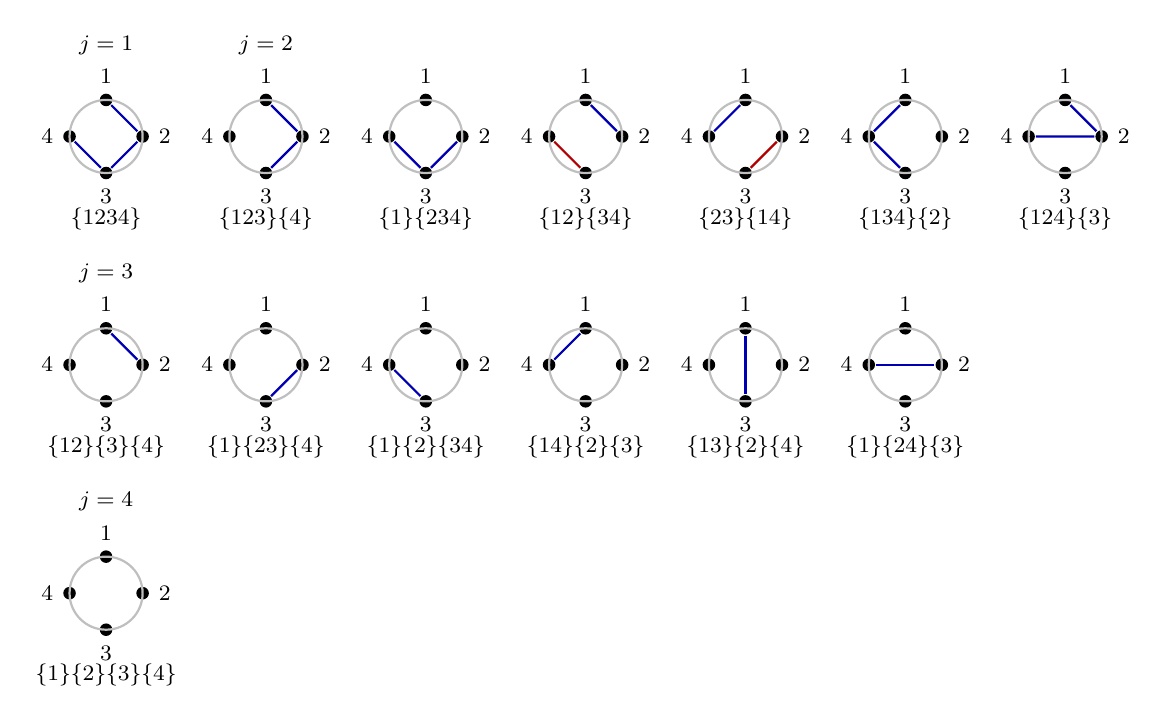
\begin{tikzpicture}[
    scale=0.58,
    node font=\footnotesize,
    dot/.style={circle, fill, inner sep=1.6pt},
    every path/.style={thick}
  ]

  \newcommand{\fournodes}[2]{%
    \node[dot,label=above:{1}]   (n1) at ([shift={(#1,#2)}]90:0.8)  {};
    \node[dot,label=right:{2}]   (n2) at ([shift={(#1,#2)}]0:0.8)   {};
    \node[dot,label=below:{3}]   (n3) at ([shift={(#1,#2)}]270:0.8) {};
    \node[dot,label=left:{4}]    (n4) at ([shift={(#1,#2)}]180:0.8) {};
    \draw[gray!50] ([shift={(#1,#2)}]0:0.8) arc(0:360:0.8);
  }

  \begin{scope}
    \fournodes{0}{0}
    \draw[blue!70!black] (n1)--(n2)--(n3)--(n4)--cycle;
    \node at (0,-1.8) {$\{1234\}$};
    \node[anchor=south] at (0,1.6) {\textbf{$j=1$}};
  \end{scope}

  \begin{scope}[xshift=3.5cm]
    \fournodes{0}{0}
    \draw[blue!70!black] (n1)--(n2)--(n3);
    \node at (0,-1.8) {$\{123\}\{4\}$};
    \node[anchor=south] at (0,1.6) {\textbf{$j=2$}};
  \end{scope}

  \begin{scope}[xshift=7cm]
    \fournodes{0}{0}
    \draw[blue!70!black] (n2)--(n3)--(n4);
    \node at (0,-1.8) {$\{1\}\{234\}$};
  \end{scope}

  \begin{scope}[xshift=10.5cm]
    \fournodes{0}{0}
    \draw[blue!70!black] (n1)--(n2);
    \draw[red!70!black] (n3)--(n4);
    \node at (0,-1.8) {$\{12\}\{34\}$};
  \end{scope}

  \begin{scope}[xshift=14cm]
    \fournodes{0}{0}
    \draw[blue!70!black] (n1)--(n4);
    \draw[red!70!black] (n2)--(n3);
    \node at (0,-1.8) {$\{23\}\{14\}$};
  \end{scope}

  \begin{scope}[xshift=17.5cm]
    \fournodes{0}{0}
    \draw[blue!70!black] (n3)--(n4)--(n1);
    \node at (0,-1.8) {$\{134\}\{2\}$};
  \end{scope}

  \begin{scope}[xshift=21cm]
    \fournodes{0}{0}
    \draw[blue!70!black] (n1)--(n2)--(n4);
    \node at (0,-1.8) {$\{124\}\{3\}$};
  \end{scope}

  \begin{scope}[yshift=-5cm]
    \fournodes{0}{0}
    \draw[blue!70!black] (n1)--(n2);
    \node at (0,-1.8) {$\{12\}\{3\}\{4\}$};
    \node[anchor=south] at (0,1.6) {\textbf{$j=3$}};
  \end{scope}

  \begin{scope}[yshift=-5cm, xshift=3.5cm]
    \fournodes{0}{0}
    \draw[blue!70!black] (n2)--(n3);
    \node at (0,-1.8) {$\{1\}\{23\}\{4\}$};
  \end{scope}

  \begin{scope}[yshift=-5cm, xshift=7cm]
    \fournodes{0}{0}
    \draw[blue!70!black] (n3)--(n4);
    \node at (0,-1.8) {$\{1\}\{2\}\{34\}$};
  \end{scope}

  \begin{scope}[yshift=-5cm, xshift=10.5cm]
    \fournodes{0}{0}
    \draw[blue!70!black] (n4)--(n1);
    \node at (0,-1.8) {$\{14\}\{2\}\{3\}$};
  \end{scope}

  \begin{scope}[yshift=-5cm, xshift=14cm]
    \fournodes{0}{0}
    \draw[blue!70!black] (n1)--(n3);
    \node at (0,-1.8) {$\{13\}\{2\}\{4\}$};
  \end{scope}

  \begin{scope}[yshift=-5cm, xshift=17.5cm]
    \fournodes{0}{0}
    \draw[blue!70!black] (n2)--(n4);
    \node at (0,-1.8) {$\{1\}\{24\}\{3\}$};
  \end{scope}

  \begin{scope}[yshift=-10cm]
    \fournodes{0}{0}
    \node at (0,-1.8) {$\{1\}\{2\}\{3\}\{4\}$};
    \node[anchor=south] at (0,1.6) {\textbf{$j=4$}};
  \end{scope}

\end{tikzpicture}
\end{adjustbox}
\caption{All 14 non-crossing partitions of $\{1,2,3,4\}$, displayed as
circle diagrams.  The elements $1,2,3,4$ are placed clockwise starting from the
top of each circle; elements within a block are connected by edges (chords or
arcs).  The partitions are organized by number of blocks $j$: one partition with
$j=1$ (Narayana number $N(4,1)=1$), six with $j=2$ ($N(4,2)=6$), six with
$j=3$ ($N(4,3)=6$), and one with $j=4$ ($N(4,4)=1$).  The single crossing
partition $\{1,3\}\{2,4\}$, whose chords would intersect, is absent.}
\label{fig16:nc4_diagrams}
\end{figure}

\subsection{The lattice diagram for \texorpdfstring{$\mathrm{NC}(3)$}{NC(3)}}

The Hasse diagram of $\mathrm{NC}(3)$ provides a compact visualization of the
partial order.  There are $C_3 = 5$ elements, arranged in three ranks.

\begin{figure}[!htbp]
\centering
\begin{adjustbox}{max width=\textwidth, center}
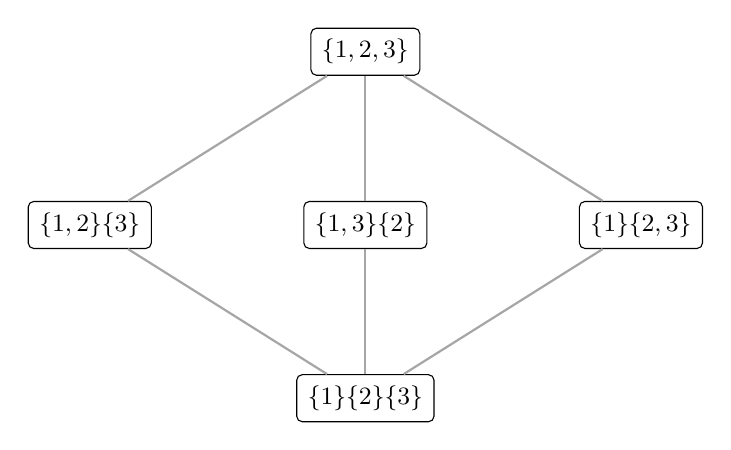
\begin{tikzpicture}[
    scale=1.0,
    every node/.style={draw, rounded corners=2pt, inner sep=4pt,
      font=\small, fill=white},
    edge/.style={thick, gray!70}
  ]
  \node (bottom) at (0,0) {$\{1\}\{2\}\{3\}$};

  \node (m1) at (-3.5,2.2) {$\{1,2\}\{3\}$};
  \node (m2) at (0,2.2)    {$\{1,3\}\{2\}$};
  \node (m3) at (3.5,2.2)  {$\{1\}\{2,3\}$};

  \node (top) at (0,4.4) {$\{1,2,3\}$};

  \draw[edge] (bottom) -- (m1);
  \draw[edge] (bottom) -- (m2);
  \draw[edge] (bottom) -- (m3);
  \draw[edge] (m1) -- (top);
  \draw[edge] (m2) -- (top);
  \draw[edge] (m3) -- (top);
\end{tikzpicture}
\end{adjustbox}
\caption{Hasse diagram of the non-crossing partition lattice $\mathrm{NC}(3)$.
The minimum element $\hat{0} = \{1\}\{2\}\{3\}$ is at the bottom; the maximum
element $\hat{1} = \{1,2,3\}$ is at the top.  The lattice is self-dual: the
Kreweras complement exchanges $\hat{0} \leftrightarrow \hat{1}$ and maps rank-1
elements to rank-1 elements.}
\label{fig16:nc3_lattice}
\end{figure}

\subsection{The role of non-crossing partitions in gravity}

In the flat-weight replica calculation, the leading Wick contractions are
labelled by non-crossing permutations, equivalently non-crossing partitions
\cite{speicher1994,voiculescu1991}.  Non-crossing pairings use a doubled set
of points under the usual bijection; they are not all pair partitions of the
original $n$ points.  The \emph{crossing} partition
$\{1,3\}\{2,4\}$ defines a genus-one Wick ribbon graph, with relative dimension suppression
$L^{-2}$ at fixed ratio.  This is not by itself a count of continuum JT handles.  The Marchenko--Pastur
distribution emerges precisely through its $n$-th moment
\begin{equation}
  m_n = \sum_{\pi \in \mathrm{NC}(n)}
  \gamma^{\,n - |\pi|}
  \label{eq16:mp_from_nc}
\end{equation}
summed over all non-crossing partitions, where $|\pi|$ counts the number of
blocks and $\gamma = k/L$ is the Hilbert-space ratio.  This is the content of
the free-probability moment--cumulant relation with free cumulants
$\kappa_m = \gamma^{m-1}$: each block $B \in \pi$ contributes
$\kappa_{|B|} = \gamma^{|B|-1}$, and the exponents add up to
$\sum_{B \in \pi} (|B|-1) = n - |\pi|$.  For $n = 2$, for example, the two
non-crossing partitions $\{12\}$ and $\{1\}\{2\}$ give
$m_2 = \gamma + 1$, the second moment of the mean-one Marchenko--Pastur law.


\section{JT Gravity: A Lightning Review}
\label{app:jt_gravity}

Jackiw--Teitelboim (JT) gravity \cite{jackiw1985,teitelboim1983} is a model of
dilaton gravity in two spacetime dimensions that has become the ``hydrogen atom''
of quantum gravity: rich enough to exhibit a gravitational path integral with
wormholes, ensemble averaging, and replica calculations, yet simple enough to
be exactly solvable.  This appendix provides the essential ingredients needed in
the main text.

\subsection{The action}

The JT gravity action consists of a topological term and a dynamical dilaton
piece:
\begin{equation}
  I_{\mathrm{JT}} = -\frac{S_0}{2\pi}
  \biggl[\frac{1}{2}\int_{\mathcal{M}} \sqrt{g}\, R
  + \int_{\partial\mathcal{M}} \sqrt{h}\, K\biggr]
  - \biggl[\frac{1}{2}\int_{\mathcal{M}} \sqrt{g}\, \phi\,(R + 2)
  + \int_{\partial\mathcal{M}} \sqrt{h}\, \phi_b\,(K-1)\biggr]\,.
  \label{eq16:jt_action}
\end{equation}
The first bracket is the two-dimensional Einstein--Hilbert action (a topological
invariant by the Gauss--Bonnet theorem), weighted by $S_0$.  On a surface of
genus $g$ with $n$ boundaries, it contributes
$-S_0\,(2 - 2g - n)/(2\pi) \times 2\pi = S_0\,(2g + n - 2)$
--- more precisely, $e^{S_0(1-2g)}$ per connected surface with one boundary.
The second bracket is the dynamical content: the dilaton field $\phi$ enforces
$R = -2$ (constant negative curvature, i.e.\ locally AdS$_2$) in the bulk, and
the boundary condition $\phi_b \to \infty$ selects asymptotically AdS$_2$
geometries.

\subsection{The Schwarzian boundary mode}

After fixing $R = -2$, the bulk geometry is rigid (locally a quotient of
$\mathbb{H}^2$), and the remaining degrees of freedom are
\emph{boundary gravitons} --- wiggles of the boundary curve in the ambient
hyperbolic disk.  These are described by a single function $f(\tau)$
parameterizing the boundary trajectory, with the effective action
\cite{maldacena2016,stanfordwitten2017}
\begin{equation}
  I_{\mathrm{Sch}}[f]
  = -C \int_0^{\beta} d\tau\;\{f,\tau\}\,,
  \qquad
  \{f,\tau\} \equiv \frac{f'''}{f'} - \frac{3}{2}
  \biggl(\frac{f''}{f'}\biggr)^{\!2}\,,
  \label{eq16:schwarzian_action}
\end{equation}
Here $f(\tau)=\tan[\pi u(\tau)/\beta]$ is a projective coordinate on the
thermal circle, with $u(\tau+\beta)=u(\tau)+\beta$.
The symbol $\{f,\tau\}$ denotes the Schwarzian derivative and
$C = \phi_r/(8\pi G_N)$ is
the ``Schwarzian coupling'' (with $\phi_r$ the renormalized boundary value of
the dilaton).  The path integral over $f$ can be performed exactly, either by
localization \cite{stanfordwitten2017} or by recognizing the Schwarzian theory
as the boundary (edge-mode) theory of two-dimensional
$\mathrm{SL}(2,\mathbb{R})$ BF~theory.

\subsection{The disk partition function}

The genus-zero, single-boundary contribution to the JT gravity partition
function is the exact Schwarzian path integral.  With Schwarzian coupling $C$,
the disk-level density of states is
\begin{equation}
  \rho_{\mathrm{disk}}(E) = e^{S_0}\;
  \frac{C\sinh\!\bigl(2\pi\sqrt{2CE}\bigr)}{2\pi^2}\,,
  \label{eq16:rho_disk}
\end{equation}
a density per unit $dE$, in the measure convention of~\citet{saadetal2019}.
An overall $C$-dependent constant can alternatively be absorbed into the
normalization of the measure; it does not affect a canonical probability at
fixed $C$.  This density of states grows
exponentially, consistent with the Bekenstein--Hawking entropy.  Its Laplace
transform, $Z(\beta) = \int_0^{\infty} dE\; \rho(E)\, e^{-\beta E}$ with
$\beta$ the inverse temperature, is Gaussian after the substitution
$E = u^2$: using
$\int_0^{\infty} \sinh\bigl(a\sqrt{E}\bigr)\, e^{-\beta E}\, dE
= \frac{\sqrt{\pi}\,a}{2\beta^{3/2}}\, e^{a^2/(4\beta)}$
with $a = 2\pi\sqrt{2C}$, one obtains the disk partition function
\begin{equation}
  Z_{\mathrm{disk}}(\beta)
  = e^{S_0}\,\frac{C^{3/2}}{\sqrt{2\pi}}\;
  \frac{e^{2\pi^{2}C/\beta}}{\beta^{3/2}}\,.
  \label{eq16:z_disk}
\end{equation}
For the entropy coordinate $x=2\pi\sqrt{2CE}$,
$E=x^2/(8\pi^2C)$ and $dE=x\,dx/(4\pi^2C)$.  Therefore the normalized
canonical distribution in that coordinate is
\begin{equation}
 p_\beta(x)=\frac{x\sinh x\,e^{-\beta x^2/(8\pi^2C)}}
 {\int_0^\infty u\sinh u\,e^{-\beta u^2/(8\pi^2C)}\,du},
 \qquad x\geq0.
 \label{eq16:jt_entropy_density}
\end{equation}
The factor $x$ is the Jacobian.  It cannot be dropped when computing entropy
fluctuations or the conditional average in Section~\ref{sec09:higher_dimensions}.

The factor $e^{S_0}$ comes from the topological term (genus $g=0$, one
boundary); the remaining factor is the exact one-loop partition function of
the Schwarzian theory.

\subsection{The matrix integral dual}

\citet{saadetal2019} match the perturbative JT amplitudes, order by order in
topology, to a double-scaled Hermitian matrix integral.  Schematically,
\begin{equation}
 \left\langle\prod_{i=1}^b Z(\beta_i)\right\rangle_{\mathrm{JT}}
 \sim\left\langle\prod_{i=1}^b\operatorname{Tr}e^{-\beta_iH}
 \right\rangle_{\mathrm{matrix}},
 \label{eq16:jt_matrix}
\end{equation}
where the equality is between the corresponding perturbative expansions.
The one-boundary disk density does not uniquely specify the nonperturbative
completion.  Such a completion requires a definition of the matrix ensemble
beyond its formal genus series.

In this formulation the path integral computes ensemble quantities rather
than directly specifying one fixed Hamiltonian.  Connected amplitudes encode
connected ensemble correlations.  A surface with two boundaries can already
be connected at genus zero, so connected fluctuations must not all be assigned
the suppression of an additional handle.  The effective counting parameter
$e^{S_0}$ organizes topology; it should not be read as the dimension of the
full continuous-energy JT Hilbert space.

\subsection{Why JT is the ``hydrogen atom'' of quantum gravity}

The analogy is apt in several respects:
\begin{enumerate}
  \item \textbf{Exact solvability.}  Just as the hydrogen atom can be solved
    exactly in quantum mechanics, JT amplitudes can be computed recursively to arbitrary perturbative order
    through the matrix-integral construction.  A specified matrix ensemble can
    additionally supply nonperturbative data.

  \item \textbf{Near-extremal applications.}  For black holes with an
    appropriate near-AdS$_2$ throat and a controlled dimensional reduction,
    JT gravity captures a leading low-energy sector.  Extra light modes,
    charges, and boundary conditions can require additional fields and change
    its range of validity~\cite{maldacena2016}.

  \item \textbf{A laboratory for ideas.}  Many central calculations in the
    Page curve program --- replica wormholes, islands, the QES formula, the
    genus expansion of entropy --- can be exhibited explicitly in JT gravity
    before attempting the (much harder) generalization to higher dimensions.

  \item \textbf{Limitations are instructive.}  JT gravity is two-dimensional,
    has no propagating gravitons, and its partition function is an ensemble
    average rather than a single-system quantity.  Understanding precisely
    \emph{where} JT gravity fails to capture higher-dimensional physics is as
    important as understanding where it succeeds.
\end{enumerate}


\section{Gaussian Broadening Integrals}
\label{app:gaussian_integrals}

The conditional entropy approximation of the main text averages the minimum
$\min(S_{\mathrm{rad}}, S_{\mathrm{BH}})$ by its average over Gaussian
fluctuations of the horizon area.  The required integrals --- the
expectations $\mathbb{E}[\max(K - X,\, 0)]$ and $\mathbb{E}[\min(X,\, K)]$
for a normal random variable $X$ --- have simple closed forms, collected in
this appendix.

\subsection{The broadening integral}

Let $X \sim \mathcal{N}(\mu, \sigma^2)$ with $\sigma > 0$, and let $K$ be a
fixed threshold.  Then
\begin{equation}
  \boxed{\;
  \mathbb{E}\bigl[\max(K - X,\, 0)\bigr]
  = (K - \mu)\,\Phi(z) + \sigma\,\phi(z)\,,
  \qquad z \equiv \frac{K - \mu}{\sigma}\,,
  \;}
  \label{eq16:gaussian_max}
\end{equation}
where $\Phi$ is the standard normal CDF and $\phi$ is the standard normal PDF.

\textbf{Derivation.}  The expectation is
\begin{align}
  \mathbb{E}[\max(K - X,\, 0)]
  &= \int_{-\infty}^{K} (K - x)\,\frac{1}{\sigma}\,
  \phi\!\Bigl(\frac{x - \mu}{\sigma}\Bigr)\, dx \nonumber \\
  &= (K - \mu)\int_{-\infty}^{K}
  \frac{1}{\sigma}\,\phi\!\Bigl(\frac{x-\mu}{\sigma}\Bigr)\, dx
  + \int_{-\infty}^{K}
  (\mu - x)\,\frac{1}{\sigma}\,
  \phi\!\Bigl(\frac{x-\mu}{\sigma}\Bigr)\, dx \nonumber \\
  &= (K - \mu)\,\Phi\!\Bigl(\frac{K-\mu}{\sigma}\Bigr)
  + \sigma \int_{-\infty}^{(K-\mu)/\sigma} (-u)\,\phi(u)\, du \nonumber \\
  &= (K - \mu)\,\Phi\!\Bigl(\frac{K-\mu}{\sigma}\Bigr)
  + \sigma\,\phi\!\Bigl(\frac{K-\mu}{\sigma}\Bigr)\,,
  \label{eq16:gaussian_max_derivation}
\end{align}
where the third line substitutes $u = (x-\mu)/\sigma$ and the final step uses
$\phi'(u) = -u\,\phi(u)$, so that the integrand of the second term is a total
derivative.  The final line agrees with the boxed
formula~\eqref{eq16:gaussian_max}.

Because $\phi$ is even and $\Phi(-z) = 1 - \Phi(z)$, the same result can be
written with the opposite sign convention $\bar{z} \equiv (\mu - K)/\sigma
= -z$:
\begin{equation}
  \mathbb{E}\bigl[\max(K - X,\, 0)\bigr]
  = (K - \mu)\,\Phi(-\bar{z}) + \sigma\,\phi(\bar{z})\,,
  \qquad \bar{z} = \frac{\mu - K}{\sigma}\,,
  \label{eq16:gaussian_max_alt}
\end{equation}
with $\bar{z} > 0$ when the mean lies above the threshold.

From the identity $\min(X,\, K) = K - \max(K - X,\, 0)$, one obtains the
companion formula
\begin{equation}
  \mathbb{E}\bigl[\min(X,\, K)\bigr]
  = K - (K - \mu)\,\Phi(z) - \sigma\,\phi(z)\,,
  \qquad z = \frac{K - \mu}{\sigma}\,.
  \label{eq16:gaussian_min}
\end{equation}
This is the form used for the conditional average of a sharp minimum.

\subsection{The Page curve as a broadened minimum}

For a conditional model with fixed radiation branch entropy
$K=S_{\mathrm{rad}}$, let $X=S_{\mathrm{BH}}$ have mean $\mu$ and variance
$\sigma^2$.  Define $\langle\Delta\rangle=K-\mu$.  The sharp conditional
average is then exactly, within the assumed Gaussian distribution,
\begin{equation}
 S_{\mathrm{diag}}^{\mathrm{sharp}}
 :=\mathbb E\min(S_{\mathrm{rad}},S_{\mathrm{BH}})
 =S_{\mathrm{rad}}-\langle\Delta\rangle
 \Phi(\langle\Delta\rangle/\sigma)
 -\sigma\phi(\langle\Delta\rangle/\sigma).
 \label{eq16:page_broadened}
\end{equation}
It tends to the minimum of the two means as $\sigma\to0$, and at equal means
has deficit $\sigma/\sqrt{2\pi}$.  The symbol $S_{\mathrm{diag}}$ records
that this is an average of conditional entropies.  It is not, without an
additional argument, the entropy of a quantum mixture of overlapping states.

The Gaussian distribution follows from a regular, locally stable saddle in
the chosen ensemble.  It does not require or establish statistically
independent Planck-area cells.  Canonically, $\operatorname{Var}E=T^2C_{\mathrm{can}}$
is exact, whereas $\delta S_{\mathrm{BH}}\simeq\delta E/T$ and
$\operatorname{Var}S_{\mathrm{BH}}\simeq C_B$ use linearization and saddle
equivalence of the heat capacities.  The thermal modular variable
$K_{\mathrm{th}}=\beta E+\log Z$ instead satisfies
$\operatorname{Var}K_{\mathrm{th}}=C_{\mathrm{can}}$ exactly.

If two subsystems exchange energy at fixed total energy, a regular saddle gives
$\operatorname{Var}E_B\simeq T^2(C_B^{-1}+C_R^{-1})^{-1}$.
Both branch entropies then fluctuate.  At equal temperatures,
$\delta(S_B-S_R)\simeq2\delta E_B/T$, so their difference has variance
$4(C_B^{-1}+C_R^{-1})^{-1}$, rather than the variance of either branch alone.
More generally the covariance term in
$\operatorname{Var}(S_B-S_R)=\operatorname{Var}S_B+
\operatorname{Var}S_R-2\operatorname{Cov}(S_B,S_R)$ must be retained.

\subsection{Non-Gaussian extensions}

Small non-Gaussian corrections about a regular saddle may be organized by an
Edgeworth expansion when the relevant cumulants possess a controlled scaling.
For a standardized variable with skewness $\zeta_3$ and excess kurtosis
$\zeta_4$, its first terms are
\begin{equation}
 f(x)\sim\phi(x)\left[1+\frac{\zeta_3}{6}H_3(x)
 +\frac{\zeta_4}{24}H_4(x)+\frac{\zeta_3^2}{72}H_6(x)+\cdots\right],
 \label{eq16:edgeworth}
\end{equation}
where the $H_j$ are probabilists' Hermite polynomials.  This is an asymptotic
expansion in the region where the saddle approximation is controlled, not a
globally positive probability density for arbitrary cumulants.  The cumulants
come from the specified probability law, not automatically from a permutation
genus coefficient.

At a critical point where the quadratic saddle term vanishes, a quartic
limiting density can be the leading law rather than a small Edgeworth
correction.  If the entropy coordinate satisfies
$X-X_c=N^{3/4}u$ and the exponent tends to $a u^4$ with $a>0$, the width
scales as $N^{3/4}$.  The Gaussian formulas above must then be replaced by
integrals against the normalized quartic density; Section~\ref{sec09:higher_dimensions}
derives the corresponding thermodynamic assumptions.


\section{Random Matrix Theory: Marchenko--Pastur and Wishart Matrices}
\label{app:rmt}

This appendix provides a self-contained derivation of the Marchenko--Pastur
(MP) distribution from several complementary perspectives.  The MP law is the
spectral law underlying the flat-weight random-state benchmark.

\subsection{Wishart matrices}

\begin{quote}
\textbf{Definition.}
Let $X$ be a $k \times L$ random matrix whose entries $X_{ij}$ are independent,
identically distributed complex Gaussian variables with mean zero and
variance $1/L$. Thus the matrix $W$ below is $1/L$ times the unit-variance
Wishart matrix in Section~\ref{sec06:replica_wormholes}. Broader sample covariance ensembles have the same leading
law under appropriate moment and independence hypotheses.  The \emph{Wishart matrix} (or \emph{sample covariance matrix}) is
\begin{equation}
  W = X X^{\dagger}\,.
  \label{eq16:wishart_def}
\end{equation}
It is a $k \times k$ positive semidefinite Hermitian matrix.  Almost surely, when $k \le L$
it has $k$ positive eigenvalues; when $k > L$ it has $L$ positive
eigenvalues and $k - L$ zero eigenvalues.
\end{quote}

The physical context is as follows.  A Haar-random pure state
$|\Psi\rangle \in \mathcal{H}_{\mathrm{rad}} \otimes \mathcal{H}_{\mathrm{BH}}$
has a reduced density matrix
$\rho_{\mathrm{rad}} = \mathrm{tr}_{\mathrm{BH}} |\Psi\rangle\langle\Psi|$
whose eigenvalues are of order $1/k$ (they sum to one).  After rescaling by
$k$, the eigenvalue distribution of $k\,\rho_{\mathrm{rad}}$ --- a mean-one spectrum, equal in law to that of
$kW/\operatorname{Tr}W$ --- converges, in the limit
$k, L \to \infty$ with $\gamma = k/L$ fixed, to the MP law
\cite{page1993, marchenkopastur1967}.

\subsection{The Marchenko--Pastur distribution}

The Marchenko--Pastur distribution with ratio parameter $\gamma > 0$ is
\begin{equation}
  \rho_{\mathrm{MP}}(\lambda)
  = \frac{\sqrt{(\lambda_{+} - \lambda)(\lambda - \lambda_{-})}}
  {2\pi\gamma\lambda}\;
  \mathbf{1}_{[\lambda_{-},\,\lambda_{+}]}(\lambda)
  + \max\!\Bigl(1 - \frac{1}{\gamma},\, 0\Bigr)\;\delta(\lambda)\,,
  \label{eq16:mp_law}
\end{equation}
where the edges are
\begin{equation}
  \lambda_{\pm} = \bigl(1 \pm \sqrt{\gamma}\bigr)^{2}\,.
  \label{eq16:mp_edges}
\end{equation}
For $\gamma < 1$ (i.e.\ $k < L$, on the smaller-radiation side) the distribution is
supported on $[\lambda_{-}, \lambda_{+}]$ with
$\lambda_{-} = (1 - \sqrt{\gamma})^2 > 0$, and there is no atom at zero.
For $\gamma > 1$ (the larger-radiation side) the continuous part is still supported
on $[\lambda_{-}, \lambda_{+}]$ with $\lambda_{-} > 0$ --- a gap
$(0, \lambda_{-})$ opens between zero and the continuous support --- and in
addition a point mass of weight $1 - 1/\gamma$ appears at $\lambda = 0$,
reflecting the $k - L$ zero eigenvalues of the rank-$L$ matrix $W$.  At the
dimension crossing $\gamma = 1$, $\lambda_{-} = 0$ and the point mass vanishes.

\subsection{Stieltjes transform derivation}
\label{app:stieltjes_derivation}

The Stieltjes transform of a probability measure $\mu$ on $\mathbb{R}$ is
\begin{equation}
  G(z) = \int \frac{d\mu(\lambda)}{z - \lambda}\,,
  \qquad z \in \mathbb{C} \setminus \mathrm{supp}(\mu)\,.
  \label{eq16:stieltjes_def}
\end{equation}
The measure can be recovered from $G$ via the Stieltjes inversion formula:
\begin{equation}
  d\mu(\lambda) = -\frac{1}{\pi}\,
  \lim_{\epsilon \to 0^{+}} \mathrm{Im}\, G(\lambda + i\epsilon)\; d\lambda\,.
  \label{eq16:stieltjes_inversion}
\end{equation}

We now derive the self-consistent equation for $G(z)$ in the Wishart case.
The resolvent of $W = XX^{\dagger}$ is
$\mathbf{G}(z) = (zI_k - W)^{-1}$, and $G(z) = \frac{1}{k}\,
\mathrm{tr}\,\mathbf{G}(z)$.

\subsubsection{Step 1: The resolvent identity}

Using the Woodbury identity (or directly from the definitions), one establishes
for the $k \times k$ resolvent:
\begin{equation}
  (zI_k - XX^{\dagger})^{-1}
  = \frac{1}{z}\,I_k
  + \frac{1}{z}\,X\,(zI_L - X^{\dagger}X)^{-1}\,X^{\dagger}\,.
  \label{eq16:woodbury}
\end{equation}
Taking $\frac{1}{k}\,\mathrm{tr}$ of both sides:
\begin{equation}
  G(z) = \frac{1}{z} + \frac{1}{z}\cdot\frac{1}{k}\,
  \mathrm{tr}\bigl[X^{\dagger}X\,(zI_L - X^{\dagger}X)^{-1}\bigr]\,.
  \label{eq16:trace_identity}
\end{equation}
Now $X^{\dagger}X$ is an $L \times L$ matrix, and its non-zero eigenvalues
coincide with those of $XX^{\dagger}$.  Denote the Stieltjes transform of the
empirical spectral distribution of $X^{\dagger}X$ by $\tilde{G}(z)$.  Then
\begin{equation}
  \frac{1}{L}\,\mathrm{tr}\,(zI_L - X^{\dagger}X)^{-1} = \tilde{G}(z)\,,
  \label{eq16:tildeG_def}
\end{equation}
and
\begin{equation}
  \frac{1}{L}\,\mathrm{tr}\bigl[X^{\dagger}X\,(zI_L - X^{\dagger}X)^{-1}\bigr]
  = -1 + z\,\tilde{G}(z)\,.
  \label{eq16:trace_manipulation}
\end{equation}
Substituting back, using $\frac{1}{k}\,\mathrm{tr} =
\frac{1}{\gamma}\cdot\frac{1}{L}\,\mathrm{tr}$ with $\gamma = k/L$:
\begin{equation}
  G(z) = \frac{1}{z}\Bigl[1 + \frac{1}{\gamma}\,
  \bigl(-1 + z\,\tilde{G}(z)\bigr)\Bigr]
  = \frac{1 - 1/\gamma}{z} + \frac{1}{\gamma}\,\tilde{G}(z)\,.
  \label{eq16:G_tildeG_relation}
\end{equation}

\subsubsection{Step 2: The self-consistency relation}

Since $XX^{\dagger}$ and $X^{\dagger}X$ share the same non-zero eigenvalues,
their Stieltjes transforms are related by
\begin{equation}
  \tilde{G}(z) = \frac{1-\gamma}{z} + \gamma\,G(z)\,,
  \label{eq16:tildeG_from_G}
\end{equation}
(accounting for the $|k - L|$ extra zero eigenvalues in the larger matrix;
this is the inverse of \eqref{eq16:G_tildeG_relation}).  These two equations
are the same eigenvalue identity and do not close the system.  Self-averaging
alone would not close it either: many deterministic spectral measures satisfy
the same relation.  The additional input is the limiting Wick moment
calculation, Eq.~\eqref{eq16:mp_from_nc}, which supplies the free cumulants
$\kappa_m=\gamma^{m-1}$.  Their generating function gives
\begin{equation}
  G(z) = \frac{1}{z - R\bigl(G(z)\bigr)}\,,
  \qquad
  R(w) = \frac{1}{1 - \gamma w}\,,
  \label{eq16:self_consistent}
\end{equation}
where $R(w)=\sum_{m\geq1}\kappa_mw^{m-1}$.  The relation between $R$ and
$G$ follows from the non-crossing moment recursion; it supplies the
probabilistic information absent from the eigenvalue identity.  Substituting $R(G) = 1/(1-\gamma G)$ and
clearing denominators,
\begin{equation}
  G\,\Bigl(z - \frac{1}{1 - \gamma G}\Bigr) = 1
  \quad \Longrightarrow \quad
  z\,G\,(1 - \gamma G) - G = 1 - \gamma G\,,
  \label{eq16:self_consistent_cleared}
\end{equation}
which rearranges to the \textbf{Marchenko--Pastur equation}:
\begin{equation}
  \boxed{\;
  \gamma z\,G^2 - (z + \gamma - 1)\,G + 1 = 0\,.
  \;}
  \label{eq16:mp_quadratic}
\end{equation}

This is a quadratic in $G$, solved by
\begin{equation}
  G(z) = \frac{(z + \gamma - 1)
  - \sqrt{(z + \gamma - 1)^2 - 4\gamma z}}{2\gamma z}\,,
  \label{eq16:mp_stieltjes}
\end{equation}
where the branch of the square root is chosen so that $G(z) \sim 1/z$ as
$z \to \infty$ (the normalization condition $\int d\mu = 1$).

\subsubsection{Step 3: Recovering the density}

The discriminant of \eqref{eq16:mp_quadratic} is
\begin{equation}
  \Delta(z) = (z + \gamma - 1)^2 - 4\gamma z
  = (z - \lambda_{+})(z - \lambda_{-})\,,
  \label{eq16:discriminant}
\end{equation}
with $\lambda_{\pm} = (1 \pm \sqrt{\gamma})^2$; expanding either side gives
$z^2 - 2(1+\gamma)z + (1-\gamma)^2$.  For real
$\lambda \in (\lambda_{-}, \lambda_{+})$, $\Delta(\lambda) < 0$ and the
square root is purely imaginary.  Applying the Stieltjes inversion formula
\eqref{eq16:stieltjes_inversion}:
\begin{equation}
  \rho(\lambda) = -\frac{1}{\pi}\,\mathrm{Im}\,G(\lambda + i0^{+})
  = \frac{\sqrt{(\lambda_{+} - \lambda)(\lambda - \lambda_{-})}}
  {2\pi\gamma\lambda}\,,
  \label{eq16:mp_density_derived}
\end{equation}
which reproduces the continuous part of \eqref{eq16:mp_law}.  For
$\gamma > 1$, the branch of \eqref{eq16:mp_stieltjes} fixed by $G \sim 1/z$
at infinity acquires a simple pole at $z = 0$ with residue $1 - 1/\gamma$,
reproducing the point mass at zero.

\subsection{\texorpdfstring{$R$}{R}-transform derivation}

The $R$-transform, introduced by Voiculescu \cite{voiculescu1991} as the
free-probability analogue of the log-characteristic function, provides an
alternative route to spectral distributions.  It is defined by
\begin{equation}
  R(w) = G^{\langle -1\rangle}(w) - \frac{1}{w}\,,
  \qquad \text{equivalently}\quad
  G\bigl(R(w) + 1/w\bigr) = w\,,
  \label{eq16:r_transform_def}
\end{equation}
where $G^{\langle -1\rangle}$ denotes the functional inverse of $G$ (so that
$G(G^{\langle -1\rangle}(w)) = w$).

The key property is \emph{additivity under free convolution}: if $a$ and $b$
are freely independent random variables, then
\begin{equation}
  R_{a+b}(w) = R_a(w) + R_b(w)\,.
  \label{eq16:r_additivity}
\end{equation}

For a Marchenko--Pastur distribution with ratio $\gamma$, the $R$-transform is
simple:
\begin{equation}
  R_{\mathrm{MP}}(w) = \frac{1}{1 - \gamma w}\,.
  \label{eq16:r_mp}
\end{equation}
Indeed, evaluating the defining relation \eqref{eq16:r_transform_def} at
$w = G(z)$ gives
\begin{equation}
  z = R(G) + \frac{1}{G} = \frac{1}{1 - \gamma G} + \frac{1}{G}\,;
  \label{eq16:r_mp_check}
\end{equation}
multiplying through by $G\,(1 - \gamma G)$ yields
$z G (1 - \gamma G) = G + (1 - \gamma G)$, which is again the quadratic
\eqref{eq16:mp_quadratic}, $\gamma z G^2 - (z + \gamma - 1)G + 1 = 0$.

The $R$-transform route is especially powerful when computing the spectral
distribution of sums of freely independent random matrices, as arises in the
analysis of the genus-zero contribution to the Page curve.

\subsection{Edge universality and Tracy--Widom fluctuations}

The MP distribution describes the \emph{bulk} eigenvalue density.  At a regular nonzero
spectral edge, the density vanishes as a square root:
$\rho(\lambda) \sim |\lambda - \lambda_{\pm}|^{1/2}$.  For complex Gaussian Wishart matrices, the edge fluctuations
have the \emph{Tracy--Widom distribution} \cite{tracywidom1994}.

Specifically, for the largest eigenvalue $\lambda_{\max}$ of a complex Gaussian
Wishart matrix at a fixed positive finite ratio:
\begin{equation}
  \frac{\lambda_{\max} - \lambda_{+}}
  {\sigma_{\mathrm{TW}}\,\min(k,L)^{-2/3}}
  \;\xrightarrow{\;d\;}\; F_2\,,
  \label{eq16:tracy_widom}
\end{equation}
where $F_2$ is the Tracy--Widom distribution for the Gaussian Unitary Ensemble
(GUE); the fluctuation scale is $\min(k,L)^{-2/3}$, and
$\sigma_{\mathrm{TW}}$ is a known $O(1)$ function of $\gamma$.

The Tracy--Widom distribution is \emph{not} Gaussian: it is asymmetric, with a
right tail that decays as $\exp\!\bigl(-\tfrac{4}{3}\,x^{3/2}\bigr)$ and a
left tail that decays as $\exp\!\bigl(-|x|^{3}/12\bigr)$.  These statements concern eigenvalues of a specified random matrix ensemble.
They do not identify eigenvalue-edge fluctuations with fluctuations of horizon
area or with competition between island saddles.  Such an identification would
require an additional derivation linking the observables and their limits.

At the special point $\gamma = 1$ (equal dimensions), the lower edge reaches the
origin: $\lambda_{-} \to 0$ while $\lambda_{+} \to 4$.  For exactly balanced dimensions, or a fixed dimension difference, the
smallest-eigenvalue limit at this hard edge is not of the
Airy-kernel (Tracy--Widom) type: they are governed by the Bessel kernel, with
limiting distributions expressible in Painlev\'e form.


\section{Selected Approaches to Black-Hole Information}
\label{app:proposals}

The approaches below supply different kinds of information: candidate
microstates, an entropy prescription, a dynamical model, interior operators,
and a geometric interpretation of entanglement. They need not be mutually
exclusive. This appendix explains the cited constructions and the questions
they address; it is not an exhaustive survey of the current status of each
research program. Section~\ref{sec13:discriminating_proposals} explains how
to formulate a quantitative comparison in a common setting.

\subsection{Fuzzballs}
\label{app:fuzzballs}

\textbf{Proponents.}  Mathur \cite{mathur2005}, Bena and Warner
\cite{benawarner2008}, and collaborators.

\medskip
\noindent
\textbf{Core idea.}  The fuzzball proposal asserts that the classical black
hole geometry is an effective description that averages over an exponentially
large number of horizon-free, horizonless solutions (``fuzzballs'' or
``microstate geometries'') in string theory.  Smooth horizonless microstate geometries are a controlled subset of the
proposed microscopic states.  The full fuzzball proposal need not describe
every state by a smooth classical geometry, and a general count of the known
smooth families has not been shown to exhaust the black-hole entropy.

\medskip
\noindent
\textbf{What has been constructed.}  Explicit microstate geometries have been
constructed for certain supersymmetric (BPS) black holes, particularly in five
dimensions:
\begin{itemize}
  \item Two-charge systems: explicit families associated with profile data
    \cite{mathur2005}.
  \item Three-charge systems: large families of ``bubbling'' geometries
    carrying the same asymptotic charges as the BMPV black hole
    \cite{benawarner2008}.
  \item Non-BPS extensions: partial constructions using ``almost-BPS'' and
    ``scaling'' solutions.
\end{itemize}

\medskip
\noindent
\textbf{What remains open.}
\begin{itemize}
  \item No complete construction of microstate geometries for the
    Schwarzschild or Kerr black holes.
  \item The ``typical'' microstate geometry (the one that dominates the
    thermodynamic ensemble) has not been identified; the known solutions are
    atypical, carrying special quantum numbers.
  \item The cited geometric constructions do not specify a normalized
    evaporation ensemble from which the radiation spectrum and its transition
    profile could be computed. That is additional dynamical input.
  \item It is unclear whether the ``fuzzball complementarity'' (the experience of an
    infalling observer) can be reconciled with a horizonless geometry.
\end{itemize}

\subsection{Islands and the replica method}
\label{app:islands}

\textbf{Proponents.}  Penington \cite{penington2020}; Almheiri, Engelhardt,
Marolf, and Maxfield \cite{almheirietal2019}; Almheiri, Mahajan, Maldacena,
and Zhao \cite{almheirietal2020islands}; Penington, Shenker, Stanford, and
Yang \cite{pssyetal2022}.

\medskip
\noindent
\textbf{Core idea.}  The island formula generalizes the quantum extremal
surface (QES) prescription \cite{engelhardtwall2015} to settings with gravity
coupled to a non-gravitational bath.  The fine-grained entropy of the radiation
is computed as
\begin{equation}
  S(\text{rad}) = \min \operatorname*{ext}_{\mathcal{I}}
  \biggl[\frac{\mathrm{Area}(\partial\mathcal{I})}{4G_N}
  + S_{\mathrm{bulk}}(\text{rad} \cup \mathcal{I})\biggr]\,,
  \label{eq16:island_formula}
\end{equation}
where $\mathcal{I}$ is the ``island'' --- a region of the black hole interior
that is entanglement-wedge reconstructable from the radiation.  In the standard evaporating examples, before the
Page time the dominant extremum is at $\mathcal{I} = \emptyset$ (no island), and
$S(\text{rad})$ grows.  After the crossing, a non-trivial island dominates and, for the
specified evaporation dynamics, gives the decreasing branch.

The replica wormhole derivation \cite{pssyetal2022} provides a
gravitational path integral justification: the island saddle is the dominant
contribution to $\overline{\mathrm{tr}(\rho^n)}$ for $n$ near 1, and the
analytic continuation to $n \to 1$ yields the island formula.

\medskip
\noindent
\textbf{What has been established.}
\begin{itemize}
  \item The island formula reproduces the Page curve in JT gravity
    coupled to a bath \cite{almheirietal2020islands, pssyetal2022}.
  \item In higher-dimensional models (Randall--Sundrum braneworlds),
    similar island calculations have been performed.
  \item The JT matrix-integral formulation organizes amplitudes by genus.
    The relation between this expansion and a particular replicated entropy
    calculation depends on its boundary conditions and normalization.
\end{itemize}

\medskip
\noindent
\textbf{What remains open.}
\begin{itemize}
  \item JT matrix-integral replica calculations compute ensemble quantities.
    Applying an ensemble result to a typical member needs a concentration
    argument; QES methods in fixed holographic theories have a broader scope
    than that particular JT ensemble interpretation.
  \item Extending a bath calculation to a fully gravitating setup requires
    specifying the radiation observable and its algebra; the tensor-factor
    treatment of the external bath cannot simply be carried over.
  \item The Page curve is one entropy statistic, not the first spectral moment
    (which is $\operatorname{Tr}\rho=1$).  R\'enyi moments and the spectral
    density already contain nontrivial planar information.  Their finite-size
    corrections require the specified model and normalization.
  \item The role of ensemble averaging vs.\ self-averaging is a central
    unresolved issue.
\end{itemize}

\subsection{Random unitary circuits and fast scrambling}
\label{app:random_unitary}

\textbf{Proponents.}  Hayden and Preskill \cite{haydenpreskill2007}; Sekino
and Susskind \cite{sekinosusskind2008}.

\medskip
\noindent
\textbf{Core idea.}  The black hole is modelled as a quantum information
processor that scrambles information via random unitary dynamics.  The Hayden--Preskill
protocol considers an old black hole (past the Page time) into which a small
diary is thrown.  If the black hole dynamics is approximated by a Haar-random
unitary, the diary's information is recoverable from the radiation after
collecting a number of additional qubits set by the diary size and desired
accuracy.  Relating this information-theoretic statement to a physical waiting
time requires a scrambling model and an emission rate.

\medskip
\noindent
\textbf{Key results.}
\begin{itemize}
  \item Hayden--Preskill: after the Page time, a Haar-random unitary acting
    on the black hole allows recovery of a diary thrown into the black hole
    from only $O(1)$ qubits of radiation beyond the diary size: after $c$
    extra quanta are collected, the recovery error is exponentially small in $c$
    \cite{haydenpreskill2007}.
  \item Sekino--Susskind: black holes motivate the fast-scrambling conjecture,
    with a scrambling time of order $\beta\log S$ \cite{sekinosusskind2008}.
  \item Approximate unitary $t$-designs: local random quantum circuits are
    proven to form approximate unitary $t$-designs in circuit depth
    polynomial in $t$ and in the number of qubits \citep{brandaoetal2016}.
    Applying such a circuit theorem to evolution generated by a particular
    chaotic Hamiltonian requires a separate argument.  This motivates --- but does not
    prove --- the Haar-random approximation used in random matrix
    calculations.
\end{itemize}

\medskip
\noindent
\textbf{What remains open.}
\begin{itemize}
  \item The Haar-random unitary model treats the black hole as a ``black box'';
    it does not provide a geometric or gravitational description of the interior.
  \item The connection between the scrambling time and the emergence of the
    island saddle in the gravitational path integral is understood heuristically
    but not rigorously.
  \item Finite-order design information controls only the corresponding copy
    moments. Additional precision and tail estimates are needed to control
    a spectral or entropy limit.
\end{itemize}

\subsection{State-dependent operators}
\label{app:state_dependent}

\textbf{Proponents.}  Papadodimas and Raju \cite{papadodimasraju2013}.

\medskip
\noindent
\textbf{Core idea.}  Papadodimas and Raju proposed that the operators
describing the black hole interior (the ``mirror operators'') must be
\emph{state-dependent}: they are defined relative to a particular equilibrium
state $|\Psi\rangle$ of the CFT and cannot be written as fixed, state-independent
operators on the Hilbert space.  This is motivated by the observation that a
state-independent construction of interior operators would violate the
basic counting of degrees of freedom (the ``AMPS'' or ``firewall'' argument
\cite{ampsetal2013}).

\medskip
\noindent
\textbf{Key features.}
\begin{itemize}
  \item The mirror operators $\tilde{O}$ are constructed as functions of the
    CFT Hamiltonian and the state $|\Psi\rangle$, acting on a ``code subspace''
    of states near $|\Psi\rangle$.
  \item Within this code subspace, the mirror operators satisfy the expected
    bulk effective field theory algebra, including the correct commutation
    relations.
  \item The construction is formulated in a large-$N$ regime; powers of $1/N$
    should not be identified with $e^{-S_0}$: it applies to low-point correlation functions in the
    large-$N$ limit.
\end{itemize}

\medskip
\noindent
\textbf{What remains open.}
\begin{itemize}
  \item State dependence is philosophically contentious: it challenges the
    standard quantum-mechanical framework in which observables are represented
    by fixed operators.
  \item Operator-algebraic approaches provide another framework for black-hole
    observables and entropy~\citep{witten2022}.  Their relation to a particular
    mirror-operator construction requires matching the states, algebras, and
    approximations; it is not an automatic reformulation of state dependence.
  \item Whether state-dependent operators can be consistently defined beyond
    perturbation theory in $1/N$ is unknown.
  \item The proposal does not directly address the Page curve; its primary
    concern is the smoothness of the black hole interior rather than the
    entropy of the radiation.
\end{itemize}

\subsection{\texorpdfstring{ER\,=\,EPR}{ER=EPR}}
\label{app:erepr}

\textbf{Proponents.}  Maldacena and Susskind \cite{maldacenasusskind2013}.

\medskip
\noindent
\textbf{Core idea.}  The ER\,=\,EPR conjecture proposes that any two
quantum systems connected by Einstein--Podolsky--Rosen (EPR) entanglement are
also connected by an Einstein--Rosen (ER) bridge (a non-traversable wormhole).
In the context of black hole evaporation, this motivates a possible geometric interpretation of correlations between
radiation and the remaining system.  Assigning a semiclassical wormhole to
each individual Hawking quantum is not an established consequence.  Geometric descriptions of more general entanglement patterns remain
conjectural outside controlled examples such as the thermofield double.

\medskip
\noindent
\textbf{Key features.}
\begin{itemize}
  \item The thermofield double state $|TFD\rangle$ of two copies of a CFT
    is dual to the two-sided eternal AdS black hole (the original ER bridge),
    providing a concrete example of ER\,=\,EPR \cite{maldacena2003}.
  \item \emph{Complexity:}  The conjecture connects entanglement to geometry
    through the concept of quantum computational complexity
    \citep{stanfordsusskind2014}.  The interior
    volume of the wormhole grows linearly in time, which is conjectured to
    be dual to the linear growth of complexity of the boundary state
    (the ``complexity = volume'' or ``complexity = action'' proposals).
  \item \emph{Traversable wormholes:}  \citet{gaoetal2017} showed that a
    double-trace deformation coupling the two boundaries of the eternal
    black hole can render the wormhole traversable.  This provides an
    operational protocol for transmitting information through the wormhole,
    which in the boundary description corresponds to quantum teleportation.
\end{itemize}

\medskip
\noindent
\textbf{What remains open.}
\begin{itemize}
  \item The unrestricted ER\,=\,EPR conjecture extends beyond the controlled
    examples described above; those examples do not establish its general form.
  \item The ``Planck-scale wormholes'' connecting individual Hawking quanta
    are far below the semiclassical regime and cannot be described by
    classical geometry.  What ``wormhole'' means in this regime is unclear.
  \item The relationship between ER\,=\,EPR and the island/replica
    approach is suggestive but not precise: the replica wormholes that
    appear in the $n$-replica calculation are Euclidean and topological,
    while the ER bridges are Lorentzian.
  \item The unrestricted conjecture does not specify a unique radiation
    channel or spectrum for comparison with another model.
\end{itemize}

\subsection{Summary: what the proposals share and where they differ}

These approaches address different questions and need not be mutually
exclusive.  Microstate geometries concern microscopic states; islands concern
entropy and reconstruction; random circuits supply dynamics in specified
models; mirror operators concern interior observables; and ER\,=\,EPR concerns
the interpretation of entanglement.  A common motivation of unitary black-hole
physics does not mean that each approach has independently calculated the same
radiation spectrum.  Quantitative comparisons require matched preparations,
observables, and approximation orders, as discussed in
Section~\ref{sec13:discriminating_proposals}.

\begin{table}[ht]
\centering
\renewcommand{\arraystretch}{1.35}
\small
\begin{adjustbox}{max width=\textwidth,center}
\begin{tabular}{@{}p{2.5cm}p{4.8cm}p{5.2cm}@{}}
\hline
\textbf{Approach} & \textbf{Construction discussed} & \textbf{Information supplied} \\
\hline
Microstate geometries &
  Explicit horizonless solutions for selected charge sectors &
  Candidate microscopic states; a complete evaporation ensemble is additional input \\
Islands and replicas &
  QES and replica calculations in specified bath-coupled models &
  Entropy and, with reconstruction arguments, a recoverable bulk algebra \\
Random unitaries &
  Haar and circuit models with a prescribed input and output split &
  Moment averages and recovery bounds for the chosen ensemble \\
Mirror operators &
  Interior operators near a selected equilibrium state &
  A local code-subspace operator algebra in the stated large-$N$ regime \\
ER\,=\,EPR &
  Two-sided AdS geometry for the thermofield double; broader conjectural extensions &
  A geometric interpretation in controlled examples, not a unique evaporation channel \\
\hline
\end{tabular}
\end{adjustbox}
\caption{Examples discussed in this appendix and the type of information each
supplies. These constructions address different questions; quantitative
comparisons require the common preparation and observable described in
Section~\ref{sec13:discriminating_proposals}.}
\label{tab16:proposals_comparison}
\end{table}


\section{Glossary of Key Terms}
\label{app:glossary}

The following terms appear frequently throughout the paper.  Definitions are
given in the context of black hole physics and the Page curve program;
mathematical terms receive their standard definitions.

\begin{description}[style=nextline, leftmargin=2.5cm, labelwidth=2.3cm]

\item[AdS/CFT]
The Anti-de~Sitter/Conformal Field Theory correspondence
\cite{maldacena1998}: a duality between a theory of quantum gravity in
$(d+1)$-dimensional Anti-de~Sitter spacetime and a conformal field theory
living on its $d$-dimensional boundary.

\item[Annealed average]
The quantity $\ln \overline{Z}$, computed by first averaging $Z$ and then
taking the logarithm.  Contrasted with the quenched
average $\overline{\ln Z}$, where the logarithm is taken before averaging.
Their difference depends on fluctuations of $Z$.  For normalized replica
moments $Z=X_n=\operatorname{Tr}\rho^n$, the corresponding entropy averages
have the same finite-dimensional limit at $n=1$.

\item[Area operator]
The area observable associated with a specified surface.  If
$S_{\mathrm{BH}}=\hat A/(4G_N)$, then
$\operatorname{Var}\hat A=16G_N^2\operatorname{Var}S_{\mathrm{BH}}$.
The further approximation $\operatorname{Var}S_{\mathrm{BH}}\simeq C_B$
requires a stable regular canonical saddle and linearization in energy.

\item[Bekenstein--Hawking entropy]
$S_{\mathrm{BH}} = A/(4G_N)$: the entropy of a black hole, proportional to
the area $A$ of the event horizon \cite{bekenstein1973, hawking1975}.

\item[Catalan number]
$C_n = \frac{1}{n+1}\binom{2n}{n}$: counts the non-crossing partitions
of $\{1,\dots,n\}$, among many other combinatorial objects.

\item[Dilaton]
A scalar field $\phi$ appearing in the JT gravity action that enforces
constant negative curvature in the bulk.  Its constant (topological) piece
$\phi_0$ sets the extremal entropy $S_0 = \phi_0/(4G_N)$, while its boundary
value $\phi_b$ sets the Schwarzian coupling $C$.

\item[Entanglement entropy]
The von~Neumann entropy $S = -\mathrm{tr}(\rho \ln \rho)$ of the reduced
density matrix of a subsystem.  For a pure global state, measures its bipartite entanglement; for a
mixed global state it also includes ordinary mixedness.

\item[ER bridge]
An Einstein--Rosen bridge: a non-traversable wormhole connecting two
asymptotic regions of a black hole spacetime.

\item[Extremal surface]
A codimension-two bulk surface with stationary area under local deformations,
subject to the prescribed anchoring and homology conditions. The HRT
prescription uses such surfaces at leading semiclassical order.

\item[Free cumulant]
The analogue of a classical cumulant in free probability.  Related to moments
by summation over non-crossing partitions (M\"obius inversion on
$\mathrm{NC}(n)$).

\item[Free probability]
A non-commutative probability theory, developed by Voiculescu
\cite{voiculescu1991}, in which the notion of independence is replaced by
\emph{free independence}.  Classical independence corresponds to tensor
products; free independence corresponds to free products.

\item[Fuzzball]
A proposed microscopic black-hole state in string theory; smooth horizonless
microstate geometries provide a controlled subset of candidate realizations \cite{mathur2005}.

\item[Genus expansion]
The perturbative expansion of the gravitational path integral (or a matrix
integral) organized by the genus $g$ of the contributing surfaces. For
connected one-boundary JT amplitudes, the convention is
$Z = \sum_g e^{(1-2g)S_0}\, Z_g$; with $b$ boundaries the topological
weight is $e^{(2-2g-b)S_0}$.

\item[Haar measure]
The unique unitarily invariant probability measure on the unitary group
$U(N)$.  Used to define ``random'' unitary operators and ``random'' pure states.

\item[Hawking radiation]
Thermal radiation emitted by a black hole due to quantum effects near the
horizon \cite{hawking1975}.  The temperature is the Hawking temperature
$T_H = \kappa_s/(2\pi)$, where $\kappa_s$ is the surface gravity.

\item[Island]
A region $\mathcal{I}$ of the black hole interior (or its entanglement wedge)
that contributes to the fine-grained entropy of the radiation via the island
formula \eqref{eq16:island_formula}.

\item[JT gravity]
Jackiw--Teitelboim gravity: a two-dimensional dilaton gravity theory.
See Appendix~\ref{app:jt_gravity}.

\item[Kreweras complement]
An anti-automorphism of the non-crossing partition lattice that maps a
partition with $j$ blocks to one with $n+1-j$ blocks.
See Appendix~\ref{app:nc_partitions}.

\item[Marchenko--Pastur distribution]
The limiting eigenvalue distribution of Wishart matrices $W = XX^{\dagger}$
(entries of $X$ i.i.d.\ with mean zero and variance $1/L$)
in the limit $k, L \to \infty$ with $\gamma = k/L$ fixed
\cite{marchenkopastur1967}.  See Appendix~\ref{app:rmt}.

\item[Narayana number]
$N(n,j) = \frac{1}{n}\binom{n}{j}\binom{n}{j-1}$: counts non-crossing
partitions of $[n]$ with exactly $j$ blocks.

\item[Non-crossing partition]
A partition of $[n]$ such that no two blocks ``cross'' when elements are
arranged on a circle.  See Appendix~\ref{app:nc_partitions}.

\item[Page curve]
The radiation entropy as a function of time.  The familiar rising and falling
profile is a typical-state benchmark for suitable evaporation models
\cite{page1993,page1993information}; unitarity alone does not fix its entire
shape or guarantee monotonic branches.

\item[Page time]
The crossing of competing entropy branches in a specified evaporation model.
In the flat-weight dimension scan it occurs at $k=L$, or $\gamma=1$.
Broadening, differing branch slopes, and finite-size corrections can shift the
maximum of the entropy away from the crossing of the branch means.

\item[Quantum extremal surface]
A codimension-two surface that extremizes generalized entropy, including the
area term and the renormalized bulk entropy. The QES prescription
\cite{engelhardtwall2015} includes quantum corrections to holographic entropy.

\item[Quenched average]
The average $\overline{\ln Z}$, where the logarithm is taken before averaging.
It is still an ensemble average, not the value of a particular realization.
For normalized density matrices the finite-dimensional quenched and annealed
replica entropies share the limit $\mathbb E S(\rho)$ at replica index one.
The entropy of the averaged matrix is a different quantity.

\item[$R$-transform]
The free-probability analogue of the logarithm of the characteristic function.
Additive under free convolution.  See Appendix~\ref{app:rmt}.

\item[R\'enyi entropy]
$S_n = \frac{1}{1-n}\ln\mathrm{tr}(\rho^n)$: a one-parameter family of
entropies that reduces to the von~Neumann entropy in the limit $n \to 1$.

\item[Replica wormhole]
A saddle-point geometry in the $n$-replica gravitational path integral that
connects different replica copies.  Replica wormholes are responsible for
the transition from the growing to the decreasing phase of the Page curve
\cite{pssyetal2022}.

\item[Scrambling time]
The time over which initially localized information becomes distributed among
many degrees of freedom.  Fast-scrambling black-hole models motivate
$t_{\mathrm{scr}}\sim\beta\log S_{\mathrm{BH}}$.  Recovery from radiation
also depends on the channel, prior entanglement, and how much radiation is collected.

\item[Schwarzian derivative]
$\{f,\tau\} = f'''/f' - \frac{3}{2}(f''/f')^2$: the differential expression
that enters the boundary action in JT gravity; see Appendix~\ref{app:jt_gravity}.

\item[Stieltjes transform]
$G(z) = \int d\mu(\lambda)/(z-\lambda)$: the analytic transform that encodes
a spectral distribution.  See Appendix~\ref{app:rmt}.

\item[Tracy--Widom distribution]
The universal distribution governing fluctuations of the largest eigenvalue
in suitable random-matrix ensembles at a regular soft edge; it is not a
general law for fluctuations of a Page transition.

\item[Wishart matrix]
A random matrix of the form $W = XX^{\dagger}$, with $X$ a $k \times L$
matrix having i.i.d.\ mean-zero entries of variance $1/L$.  Models the
(rescaled) reduced density matrix of a random pure state.

\end{description}


\begin{thebibliography}{99}
\bibitem[Almheiri et~al.(2020b)]{ahmstetal2020}
Almheiri, A., T.~Hartman, J.~Maldacena, E.~Shaghoulian, and A.~Tajdini, 2020, Replica Wormholes and the Entropy of Hawking Radiation, \textit{Journal of High Energy Physics} 2020, 013.

\bibitem[Almheiri et~al.(2021)]{ahmstetal2021}
Almheiri, A., T.~Hartman, J.~Maldacena, E.~Shaghoulian, and A.~Tajdini, 2021, The Entropy of Hawking Radiation, \textit{Reviews of Modern Physics} 93, 035002.

\bibitem[Akers and Penington(2021)]{akerspenington2021}
Akers, C., and G.~Penington, 2021, Leading Order Corrections to the Quantum Extremal Surface Prescription, \textit{Journal of High Energy Physics} 2021, 062.

\bibitem[Almheiri et~al.(2019)]{almheirietal2019}
Almheiri, A., N.~Engelhardt, D.~Marolf, and H.~Maxfield, 2019, The Entropy of Bulk Quantum Fields and the Entanglement Wedge of an Evaporating Black Hole, \textit{Journal of High Energy Physics} 2019, 063.

\bibitem[Almheiri et~al.(2020a)]{almheirietal2020islands}
Almheiri, A., R.~Mahajan, J.~Maldacena, and Y.~Zhao, 2020, The Page Curve of Hawking Radiation from Semiclassical Geometry, \textit{Journal of High Energy Physics} 2020, 149.

\bibitem[Almheiri et~al.(2013)]{ampsetal2013}
Almheiri, A., D.~Marolf, J.~Polchinski, and J.~Sully, 2013, Black Holes: Complementarity or Firewalls?, \textit{Journal of High Energy Physics} 2013, 062.

\bibitem[Araki and Lieb(1970)]{arakilieb1970}
Araki, H., and E.~H.~Lieb, 1970, Entropy Inequalities, \textit{Communications in Mathematical Physics} 18, 160--170.

\bibitem[Bachelier(1900)]{bachelier1900}
Bachelier, L., 1900, Th\'{e}orie de la Sp\'{e}culation, \textit{Annales Scientifiques de l'\'{E}cole Normale Sup\'{e}rieure} 17, 21--86.

\bibitem[Balasubramanian et~al.(2024)]{balasubramanianetal2024}
Balasubramanian, V., A.~Lawrence, J.~M.~Mag\'{a}n, and M.~Sasieta, 2024, Microscopic Origin of the Entropy of Black Holes in General Relativity, \textit{Physical Review X} 14, 011024.

\bibitem[Banks et~al.(1984)]{banks1984}
Banks, T., L.~Susskind, and M.~E.~Peskin, 1984, Difficulties for the Evolution of Pure States into Mixed States, \textit{Nuclear Physics B} 244, 125--134.

\bibitem[Bardeen et~al.(1973)]{bardeenetal1973}
Bardeen, J.~M., B.~Carter, and S.~W.~Hawking, 1973, The Four Laws of Black Hole Mechanics, \textit{Communications in Mathematical Physics} 31, 161--170.

\bibitem[Bekenstein(1973)]{bekenstein1973}
Bekenstein, J.~D., 1973, Black Holes and Entropy, \textit{Physical Review D} 7, 2333--2346.

\bibitem[Bell(1964)]{bell1964}
Bell, J.~S., 1964, On the Einstein Podolsky Rosen Paradox, \textit{Physics Physique Fizika} 1, 195--200.

\bibitem[Bena and Warner(2008)]{benawarner2008}
Bena, I., and N.~P.~Warner, 2008, Black Holes, Black Rings, and their Microstates, \textit{Lecture Notes in Physics} 755, 1--92.

\bibitem[Bousso and Miyaji(2024)]{boussomiyaji2024}
Bousso, R., and M.~Miyaji, 2024, Fluctuations in the Entropy of Hawking Radiation,
\textit{Physical Review D} 109, 026006, arXiv:2307.13920.

\bibitem[Brand\~{a}o et~al.(2016)]{brandaoetal2016}
Brand\~{a}o, F.~G.~S.~L., A.~W.~Harrow, and M.~Horodecki, 2016, Local Random Quantum Circuits Are Approximate Polynomial-Designs, \textit{Communications in Mathematical Physics} 346, 397--434.

\bibitem[Calabrese and Cardy(2004)]{calabresecardy2004}
Calabrese, P., and J.~Cardy, 2004, Entanglement Entropy and Quantum Field Theory, \textit{Journal of Statistical Mechanics: Theory and Experiment} 2004, P06002.

\bibitem[Carlson(1914)]{carlson1914}
Carlson, F., 1914, Sur une Classe de S\'{e}ries de Taylor, Ph.D. thesis, Uppsala University.

\bibitem[Carter(1971)]{carter1971}
Carter, B., 1971, Axisymmetric Black Hole Has Only Two Degrees of Freedom, \textit{Physical Review Letters} 26, 331--333.

\bibitem[Chamblin et al.(1999)]{chamblin1999}
A.~Chamblin, R.~Emparan, C.~V.~Johnson and R.~C.~Myers,
\emph{Charged AdS black holes and catastrophic holography},
Phys.\ Rev.\ D \textbf{60} (1999) 064018
[\href{https://arxiv.org/abs/hep-th/9902170}{hep-th/9902170}].

\bibitem[Cheng et~al.(2024)]{chengetal2024}
Cheng, N., Lancien, C., Penington, G., Walter, M., and Witteveen, F., 2024, Random Tensor Networks with Non-trivial Links, \textit{Annales Henri Poincar\'{e}} 25(4), 2107--2212.

\bibitem[Choi(1975)]{choi1975}
Choi, M.-D., 1975, Completely positive linear maps on complex matrices,
\textit{Linear Algebra and its Applications} 10, 285--290,
doi:10.1016/0024-3795(75)90075-0.

\bibitem[Coffman et~al.(2000)]{coffmanetal2000}
Coffman, V., J.~Kundu, and W.~K.~Wootters, 2000, Distributed Entanglement, \textit{Physical Review A} 61, 052306.

\bibitem[Colin-Ellerin et~al.(2021)]{colinetal2021}
Colin-Ellerin, S., X.~Dong, D.~Marolf, M.~Rangamani, and Z.~Wang, 2021, Real-Time Gravitational Replicas: Formalism and a Variational Principle, \textit{Journal of High Energy Physics} 2021, 117.

\bibitem[Cori and Hetyei(2014)]{corihetyei2014}
Cori, R., and G.~Hetyei, 2014, Counting genus one partitions and permutations,
\textit{S\'eminaire Lotharingien de Combinatoire} 70, B70e, arXiv:1306.4628.

\bibitem[Dong and Wang(2020)]{dongwang2020}
X.~Dong and H.~Wang, \emph{Enhanced corrections near holographic entanglement transitions: a chaotic case study},
JHEP \textbf{11} (2020) 007
[\href{https://arxiv.org/abs/2006.10051}{2006.10051}].

\bibitem[Engelhardt and Wall(2015)]{engelhardtwall2015}
Engelhardt, N., and A.~C.~Wall, 2015, Quantum Extremal Surfaces: Holographic Entanglement Entropy beyond the Classical Regime, \textit{Journal of High Energy Physics} 2015, 073.

\bibitem[Faulkner et~al.(2013)]{faulkneretal2013}
Faulkner, T., A.~Lewkowycz, and J.~Maldacena, 2013, Quantum Corrections to Holographic Entanglement Entropy, \textit{Journal of High Energy Physics} 2013, 074.

\bibitem[Feynman(1948)]{feynman1948}
Feynman, R.~P., 1948, Space-Time Approach to Non-Relativistic Quantum Mechanics, \textit{Reviews of Modern Physics} 20, 367--387.

\bibitem[Gao et~al.(2017)]{gaoetal2017}
Gao, P., D.~L.~Jafferis, and A.~C.~Wall, 2017, Traversable Wormholes via a Double Trace Deformation, \textit{Journal of High Energy Physics} 2017, 151.

\bibitem[Gibbons and Hawking(1977)]{gibbonshawking1977}
Gibbons, G.~W., and S.~W.~Hawking, 1977, Action Integrals and Partition Functions in Quantum Gravity, \textit{Physical Review D} 15, 2752--2756.

\bibitem[Giddings(1992)]{giddings1992}
Giddings, S.~B., 1992, Black Holes and Massive Remnants, \textit{Physical Review D} 46, 1347--1352.

\bibitem[Giraud(2007)]{giraud2007}
Giraud, O., 2007, Distribution of bipartite entanglement for random pure states,
\textit{J.\ Phys.\ A: Math.\ Theor.} 40, 2793--2801,
doi:10.1088/1751-8113/40/11/014, arXiv:quant-ph/0611285.

\bibitem[Goupil and Schaeffer(1998)]{goupilschaeffer1998}
Goupil, A., and G.~Schaeffer, 1998, Factoring $n$-cycles and counting maps of given genus,
\textit{European Journal of Combinatorics} 19, 819--834.

\bibitem[Harer and Zagier(1986)]{harerzagier1986}
Harer, J., and D.~Zagier, 1986, The Euler characteristic of the moduli space of curves, \textit{Inventiones Mathematicae} 85, 457--485.

\bibitem[Harlow(2016)]{harlow2016}
Harlow, D., 2016, Jerusalem Lectures on Black Holes and Quantum Information, \textit{Reviews of Modern Physics} 88, 015002.

\bibitem[Hawking(1971)]{hawking1971area}
Hawking, S.~W., 1971, Gravitational Radiation from Colliding Black Holes, \textit{Physical Review Letters} 26, 1344--1346.

\bibitem[Hawking(1975)]{hawking1975}
Hawking, S.~W., 1975, Particle Creation by Black Holes, \textit{Communications in Mathematical Physics} 43, 199--220.

\bibitem[Hawking(1976)]{hawking1976}
Hawking, S.~W., 1976, Breakdown of Predictability in Gravitational Collapse, \textit{Physical Review D} 14, 2460--2473.

\bibitem[Hawking and Page(1983)]{hawkingpage1983}
Hawking, S.~W., and D.~N.~Page, 1983, Thermodynamics of Black Holes in Anti-de Sitter Space, \textit{Communications in Mathematical Physics} 87, 577--588.

\bibitem[Hayden and Preskill(2007)]{haydenpreskill2007}
Hayden, P., and J.~Preskill, 2007, Black Holes as Mirrors: Quantum Information in Random Subsystems, \textit{Journal of High Energy Physics} 2007, 120.

\bibitem[Holevo(1973)]{holevo1973}
Holevo, A.~S., 1973, Bounds for the Quantity of Information Transmitted by a
Quantum Communication Channel, \textit{Problems of Information Transmission}
9, 177--183.

\bibitem[Hubeny et~al.(2007)]{hubenyetal2007}
Hubeny, V.~E., M.~Rangamani, and T.~Takayanagi, 2007, A Covariant Holographic Entanglement Entropy Proposal, \textit{Journal of High Energy Physics} 2007, 062.

\bibitem[Islam et~al.(2015)]{islametal2015}
Islam, R., R.~Ma, P.~M.~Preiss, M.~E.~Tai, A.~Lukin, M.~Rispoli, and M.~Greiner, 2015, Measuring Entanglement Entropy in a Quantum Many-Body System, \textit{Nature} 528, 77--83.

\bibitem[Israel(1967)]{israel1967}
Israel, W., 1967, Event Horizons in Static Vacuum Space-Times, \textit{Physical Review} 164, 1776--1779.

\bibitem[Israel(1968)]{israel1968}
Israel, W., 1968, Event Horizons in Static Electrovac Space-Times, \textit{Communications in Mathematical Physics} 8, 245--260.

\bibitem[Jackiw(1985)]{jackiw1985}
Jackiw, R., 1985, Lower Dimensional Gravity, \textit{Nuclear Physics B} 252, 343--356.

\bibitem[Kreweras(1972)]{kreweras1972}
Kreweras, G., 1972, Sur les Partitions Non Crois\'{e}es d'un Cycle, \textit{Discrete Mathematics} 1, 333--350.

\bibitem[Kubiznak and Mann(2012)]{kubiznakmann2012}
D.~Kubiz\v{n}\'{a}k and R.~B.~Mann, \emph{$P$--$V$ criticality of charged AdS black holes},
JHEP \textbf{07} (2012) 033
[\href{https://arxiv.org/abs/1205.0559}{1205.0559}].

\bibitem[Lewkowycz and Maldacena(2013)]{lewkowyczmaldacena2013}
Lewkowycz, A., and J.~Maldacena, 2013, Generalized Gravitational Entropy, \textit{Journal of High Energy Physics} 2013, 090.

\bibitem[Lieb and Ruskai(1973)]{liebruskai1973}
Lieb, E.~H., and M.~B.~Ruskai, 1973, Proof of the Strong Subadditivity of Quantum-Mechanical Entropy, \textit{Journal of Mathematical Physics} 14, 1938--1941.

\bibitem[Lloyd and Pagels(1988)]{lloydpagels1988}
Lloyd, S., and H.~Pagels, 1988, Complexity as Thermodynamic Depth, \textit{Annals of Physics} 188, 186--213.

\bibitem[Lubkin(1978)]{lubkin1978}
Lubkin, E., 1978, Entropy of an n-System from Its Correlation with a k-Reservoir, \textit{Journal of Mathematical Physics} 19, 1028--1031.

\bibitem[Maldacena(1998)]{maldacena1998}
Maldacena, J., 1998, The Large $N$ Limit of Superconformal Field Theories and Supergravity, \textit{Advances in Theoretical and Mathematical Physics} 2, 231--252.

\bibitem[Maldacena(2003)]{maldacena2003}
Maldacena, J., 2003, Eternal Black Holes in Anti-de Sitter, \textit{Journal of High Energy Physics} 2003, 021.

\bibitem[Maldacena et~al.(2016)]{maldacena2016}
Maldacena, J., D.~Stanford, and Z.~Yang, 2016, Conformal Symmetry and its Breaking in Two Dimensional Nearly Anti-de-Sitter Space, \textit{Progress of Theoretical and Experimental Physics} 2016, 12C104.

\bibitem[Maldacena and Susskind(2013)]{maldacenasusskind2013}
Maldacena, J., and L.~Susskind, 2013, Cool Horizons for Entangled Black Holes, \textit{Fortschritte der Physik} 61, 781--811.

\bibitem[Marchenko and Pastur(1967)]{marchenkopastur1967}
Marchenko, V.~A., and L.~A.~Pastur, 1967, Distribution of Eigenvalues for Some Sets of Random Matrices, \textit{Matematicheskii Sbornik} 72, 507--536.

\bibitem[Markov(1958)]{markov1958}
Markov, A.~A., 1958, Insolubility of the Problem of Homeomorphy, in \textit{Proceedings of the International Congress of Mathematicians 1958} (Cambridge University Press), 300--306.

\bibitem[Marolf and Maxfield(2020)]{marolfmaxfield2020}
Marolf, D., and H.~Maxfield, 2020, Transcending the Ensemble: Baby Universes, Spacetime Wormholes, and the Order and Disorder of Black Hole Information, \textit{Journal of High Energy Physics} 2020, 044.

\bibitem[Marolf et~al.(2020)]{marolfwangwang2020}
Marolf, D., Wang, S., and Wang, Z., 2020, Probing Phase Transitions of Holographic Entanglement Entropy with Fixed Area States, \textit{Journal of High Energy Physics} 2020(12), 084.

\bibitem[Mathur(2005)]{mathur2005}
Mathur, S.~D., 2005, The Fuzzball Proposal for Black Holes: an Elementary Review, \textit{Fortschritte der Physik} 53, 793--827.

\bibitem[Mathur(2009)]{mathur2009}
Mathur, S.~D., 2009, The information paradox: A pedagogical introduction,
\textit{Classical and Quantum Gravity} 26, 224001, arXiv:0909.1038.

\bibitem[Mertens and Turiaci(2023)]{mertensturiaci2023}
Mertens, T.~G., and G.~J.~Turiaci, 2023, Solvable Models of Quantum Black Holes: A Review on Jackiw--Teitelboim Gravity, \textit{Living Reviews in Relativity} 26, 4.

\bibitem[M\"uck(2024)]{muck2024}
M\"uck, W., 2024, Black holes and Marchenko--Pastur distribution, \textit{Physical Review D} 109, 126001.

\bibitem[Murthy and Srednicki(2019)]{murthysrednicki2019}
Murthy, C. and Srednicki, M., 2019, Structure of Chaotic Eigenstates and Their Entanglement Entropy, \textit{Physical Review E} 100, 022131.

\bibitem[Nielsen and Chuang(2000)]{nielsen2000}
Nielsen, M.~A., and I.~L.~Chuang, 2000, \textit{Quantum Computation and Quantum Information} (Cambridge University Press, Cambridge).

\bibitem[Osterwalder and Schrader(1973)]{osterwalderschrader1973}
Osterwalder, K., and R.~Schrader, 1973, Axioms for Euclidean Green's Functions, \textit{Communications in Mathematical Physics} 31, 83--112.

\bibitem[Osterwalder and Schrader(1975)]{osterwalderschrader1975}
Osterwalder, K., and R.~Schrader, 1975, Axioms for Euclidean Green's Functions II, \textit{Communications in Mathematical Physics} 42, 281--305.

\bibitem[Page(1976)]{page1976}
Page, D.~N., 1976, Particle Emission Rates from a Black Hole: Massless Particles from an Uncharged, Nonrotating Hole, \textit{Physical Review D} 13, 198--206.

\bibitem[Page(1993a)]{page1993}
Page, D.~N., 1993, Average Entropy of a Subsystem, \textit{Physical Review Letters} 71, 1291--1294.

\bibitem[Page(1993b)]{page1993information}
Page, D.~N., 1993, Information in Black Hole Radiation, \textit{Physical Review Letters} 71, 3743--3746.

\bibitem[Papadodimas and Raju(2013)]{papadodimasraju2013}
Papadodimas, K., and S.~Raju, 2013, An Infalling Observer in AdS/CFT, \textit{Journal of High Energy Physics} 2013, 212.

\bibitem[Penington(2020)]{penington2020}
Penington, G., 2020, Entanglement Wedge Reconstruction and the Information Paradox, \textit{Journal of High Energy Physics} 2020, 002.

\bibitem[Penrose(1963)]{penrose1963}
Penrose, R., 1963, Asymptotic Properties of Fields and Space-Times, \textit{Physical Review Letters} 10, 66--68.

\bibitem[Penington et~al.(2022)]{pssyetal2022}
Penington, G., S.~H.~Shenker, D.~Stanford, and Z.~Yang, 2022, Replica Wormholes and the Black Hole Interior, \textit{Journal of High Energy Physics} 2022, 205.

\bibitem[Raju(2022)]{raju2022}
Raju, S., 2022, Lessons from the Information Paradox, \textit{Physics Reports} 943, 1--80.

\bibitem[Ryu and Takayanagi(2006)]{ryutakayanagi2006}
Ryu, S., and T.~Takayanagi, 2006, Holographic Derivation of Entanglement Entropy from the anti-de Sitter Space/Conformal Field Theory Correspondence, \textit{Physical Review Letters} 96, 181602.

\bibitem[Saad et~al.(2019)]{saadetal2019}
Saad, P., S.~H.~Shenker, and D.~Stanford, 2019, JT Gravity as a Matrix Integral, arXiv:1903.11115.

\bibitem[Sakurai and Napolitano(2020)]{sakurai2020}
Sakurai, J.~J., and J.~Napolitano, 2020, \textit{Modern Quantum Mechanics}, 3rd ed.\ (Cambridge University Press, Cambridge).

\bibitem[Schumacher(1996)]{schumacher1996}
Schumacher, B., 1996, Sending entanglement through noisy quantum channels,
\textit{Physical Review A} 54, 2614--2628,
doi:10.1103/PhysRevA.54.2614, arXiv:quant-ph/9604023.

\bibitem[Schwarzschild(1916)]{schwarzschild1916}
Schwarzschild, K., 1916, \"{U}ber das Gravitationsfeld eines Massenpunktes nach der Einsteinschen Theorie, \textit{Sitzungsberichte der K\"{o}niglich Preu{\ss}ischen Akademie der Wissenschaften} 189--196.

\bibitem[Sekino and Susskind(2008)]{sekinosusskind2008}
Sekino, Y., and L.~Susskind, 2008, Fast Scramblers, \textit{Journal of High Energy Physics} 2008, 065.

\bibitem[Sen(1996)]{sen1996}
Sen, S., 1996, Average Entropy of a Quantum Subsystem,
\textit{Physical Review Letters} 77, 1--3, arXiv:hep-th/9601132.

\bibitem[Speicher(1994)]{speicher1994}
Speicher, R., 1994, Multiplicative Functions on the Lattice of Non-Crossing Partitions and Free Convolution, \textit{Mathematische Annalen} 298, 611--628.

\bibitem[Speicher(1997)]{speicher1997}
Speicher, R., 1997, Free Probability Theory and Non-Crossing Partitions, \textit{S\'{e}minaire Lotharingien de Combinatoire} 39, B39c.

\bibitem[Stanford and Susskind(2014)]{stanfordsusskind2014}
Stanford, D., and L.~Susskind, 2014, Complexity and Shock Wave Geometries, \textit{Physical Review D} 90, 126007.

\bibitem[Stanford and Witten(2017)]{stanfordwitten2017}
Stanford, D., and E.~Witten, 2017, Fermionic Localization of the Schwarzian Theory, \textit{Journal of High Energy Physics} 2017, 008.

\bibitem[Susskind(1995)]{susskind1995}
Susskind, L., 1995, The World as a Hologram, \textit{Journal of Mathematical Physics} 36, 6377--6396.

\bibitem[Teitelboim(1983)]{teitelboim1983}
Teitelboim, C., 1983, Gravitation and Hamiltonian Structure in Two Spacetime Dimensions, \textit{Physics Letters B} 126, 41--45.

\bibitem['t~Hooft(1974)]{thooft1974}
't~Hooft, G., 1974, A Planar Diagram Theory for Strong Interactions, \textit{Nuclear Physics B} 72, 461--473.

\bibitem['t~Hooft(1993)]{thooft1993}
't~Hooft, G., 1993, Dimensional Reduction in Quantum Gravity, in \textit{Salamfestschrift}, edited by A.~Ali, J.~Ellis, and S.~Randjbar-Daemi, World Scientific, pp.~284--296.

\bibitem[Tracy and Widom(1994)]{tracywidom1994}
Tracy, C.~A., and H.~Widom, 1994, Level-Spacing Distributions and the Airy Kernel, \textit{Communications in Mathematical Physics} 159, 151--174.

\bibitem[Vidmar and Rigol(2017)]{vidmarrigol2017}
Vidmar, L. and Rigol, M., 2017, Entanglement Entropy of Eigenstates of Quantum Chaotic Hamiltonians, \textit{Physical Review Letters} 119, 220603.

\bibitem[Voiculescu(1991)]{voiculescu1991}
Voiculescu, D., 1991, Limit Laws for Random Matrices and Free Products, \textit{Inventiones Mathematicae} 104, 201--220.

\bibitem[Wang(2023)]{wang2023}
Wang, J., 2023, Beyond Islands: A Free Probabilistic Approach, \textit{Journal of High Energy Physics} 2023(10), 040.

\bibitem[Witten(1998)]{witten1998}
E.~Witten, \emph{Anti-de Sitter space, thermal phase transition, and confinement in gauge theories},
Adv.\ Theor.\ Math.\ Phys.\ \textbf{2} (1998) 505--532
[\href{https://arxiv.org/abs/hep-th/9803131}{hep-th/9803131}].

\bibitem[Witten(2022)]{witten2022}
Witten, E., 2022, Gravity and the Crossed Product, \textit{Journal of High Energy Physics} 2022, 008.

\bibitem[Wuebben(2026a)]{wuebben2026paper1}
Wuebben, B.~J., 2026, The Page Curve Through the Transition: An Order-One Correction to the Diagonal Approximation, preprint.

\bibitem[Wuebben(2026b)]{wuebben2026paper2}
Wuebben, B.~J., 2026, The Page Curve in Higher Dimensions: Phase Transitions, Critical Phenomena, and Finite-Size Broadening, preprint.

\bibitem[Wuebben(2026c)]{wuebben2026paper3}
Wuebben, B.~J., 2026, The Page Curve Is Not Enough: Universality, Ensemble Dependence, and Microscopic Ambiguity in Black Hole Information Recovery, preprint.

\bibitem[York(1972)]{york1972}
York, J.~W., Jr., 1972, Role of Conformal Three-Geometry in the Dynamics of Gravitation, \textit{Physical Review Letters} 28, 1082--1085.

\bibitem[York(1986)]{york1986}
J.~W.~York, Jr., \emph{Black-hole thermodynamics and the Euclidean Einstein action},
Phys.\ Rev.\ D \textbf{33} (1986) 2092,
\href{https://doi.org/10.1103/PhysRevD.33.2092}{doi:10.1103/PhysRevD.33.2092}.

\end{thebibliography}

\end{document}
